\documentclass[]{FZGdasa}
\usepackage{comment}

%Options > Configure TeXstudio > Build > Default Bibliography Tool
% SET IT TO biber!!! not bibtex

% {Klassen} entspr. *.cls Dateien:
% FZGdasa > arbeitet mit \chapter als höchste Ebene
%
% [Optionen]:
% entwurf      > Erstelldatum, Anmerkungen usw. sichtbar
% notoc        > kein Inhaltsverzeichnis
% nokeys       > keine labels anzeigen im entwurf-Modus
% notodolist   > keine Auflistung der mit \Note \sNote \Explain \Reminder \sReminder gekennzeichneten Stellen
% noxurl       > kein Zeilenumbruch in URL an alphanumerischen Zeichen, aber Skalierung des Zeichenabstands in URL in Literaturverzeichnis
% english

% Schlüsselwörter:
\Arbeit{Semesterarbeit}
\Nummer{1888}
\ThemaDeutsch{Erweiterte Konfidenzbetrachtung des Schädigungszustands von	Maschinenelementen mittels Methoden des Maschinellen Lernens}
\ThemaEnglisch{Advanced Confidence Analysis of the State of Damage of Machine Elements Utilizing Machine Learning}
%\ErlangungGrad{B.Sc./M.Sc. (entfällt bei Semesterarbeit)}
\AutorAnrede{Herr}
\Autorname{Jan Nalivaika, B.Sc.}
\AutorMatrNr{03694590}
\Betreuername{Daniel Vietze, M.Sc.}
\Themenstellername[Prof. Dr.-Ing.]{Karsten Stahl}
\ThemenstellerZusatz{Lehrstuhl für Maschinenelemente}
\Beginn{19.04.2023}
\Ende{19.09.2023}
\Ort{Garching bei München}
\Aufgabepfad{aufgabenstellung.tex}

% Verfügbare Kommandos:
%\siehe[1]{s.~#1}
%{\chapref}[1]{\textbf{\chaptername~\ref{#1}}}
%{\schapref}[1]{\siehe{\chapref{#1}}}
%{\secref}[1]{\textbf{Abschnitt~\ref{#1}}}
%{\ssecref}[1]{\siehe{\secref{#1}}}
%{\eqref}[1]{\textbf{Formel~(\ref{#1})}}
%{\seqref}[1]{\siehe{\eqref{#1}}}
%{\figref}[1]{\textbf{\figurename~\ref{#1}}}
%{\sfigref}[1]{\siehe{\figref{#1}}}
%{\tabref}[1]{\textbf{\tablename~\ref{#1}}}
%{\stabref}[1]{\siehe{\tabref{#1}}}
%{\datref}[1]{\textbf{Dateifenster~\ref{#1}}}
%{\sdatref}[1]{\siehe{\datef{#1}}}

%\addbibresource{litbib.bib}

\begin{document}


% !TeX spellcheck = en_US 
\chapter{Introduction}
\section{Motivation}\label{intro}
As “Industrie 4.0” became the new standard, more and more data is continuously gathered in every industry process \cite{Vogel}. By analyzing this large amount of data, new options are discovered and implemented that can help save resources, time, and money~\cite{Theodoridis}. The use-cases range from yield improvement in chemical processes, condition monitoring in machinery, to fraud detection in banking~\cite{Janiesch}. New insight from that data enables more specialized solutions and significantly faster improvements in almost all processes~\cite{Russell}. 

To analyze the gathered data, more and more sophisticated methods have been developed over the last few years. Not only did the available computing power take a significant leap forward, but also the methods for data analysis and knowledge extrapolation, which are now widely available~\cite{Janiesch}. One of the most prominent methods is Machine Learning (ML) which is part of Artificial Intelligence (AI) \cite{Helm}. Since the early beginnings of AI in 1956, the idea of ML has gotten more and more public attention \cite{Russell}. Today, ML is applied in all areas where traditional algorithms cannot handle the amount of data or the problems are too abstract~\cite{Carleo}. Image recognition and chatbots are just a small example of the possibilities ML is able to offer~\cite{Theodoridis}.
%Especially as the computing capabilities of household computers are now far more capable and affordable. Chat-GPT is one of the latest advancements that received much public attention for the ability to interact with a human through a chat-interface and answer various questions with very precise accuracy. 

Especially engineering sciences are interested in the implementation of ML and the associated improvement of processes~\cite{Carleo}. Saving money by optimizing processes and workflows is one of the biggest driving forces for ML. In more and more use cases, like predictive maintenance and anomaly detection, ML is the new normal~\cite{Theodoridis}.

Gears are one of the most common elements in mechanical engineering and can be found in almost every part of industry applications~\cite{Vullo}. Those gears are dimensioned, manufactured, and treated in such a way as to require the least amount of material and still fulfill their purpose without failure throughout their desired lifetime \cite{Bugliarello}. This thesis takes a deeper look at how the application of ML can support the confidence in the calculated current state-of-damage by specifically considering the time history of the loads applied onto the gear.
\section{Problem and Goal Formulation}
\subsection{Problem Statement}\label{prob}

In mechanical engineering, machine elements are usually designed to withstand loads in an expected range over their desired course of life \cite{Vietze}. Those loads are mostly not static but dynamic and can vary significantly in their magnitude over the operating time \cite{Wittel}. For example, gears in a car's transmission or gearbox experience a variety of loads depending on the torque output of the engine \cite{Yuksel}. Rapid acceleration with a heavy trailer has a different time-load profile than just cruising at constant speed.
\newpage
To determine the current state-of-damage, multiple methods can be employed \cite{Lee}. One of the most used methods is the Miner rule \cite{MinerOG} (also called the Palmgren-Miner rule) which is one option of the linear approaches \cite{Sun}. The Miner rule is also referred to in international standards \cite{ISO1}.

One of its main advantages is its simplicity and general applicability. The Miner rule assumes that each load cycle is responsible for a certain percentage of damage. Higher loads are responsible for more damage. The accumulated damage for one load level is proportional to its applied cycles. A machine element is expected to fail as soon as the accumulated damage~sum~D reaches 1.0 (also referred to as unity) \cite{ISO1, Miller}.

When comparing this approach to experiments, it is shown that the Miner rule does not always correctly calculate the true physical state-of-damage \cite{Pavlou}. For example, multiple experiments were conducted with gears that showed that the damage sum D, calculated with the Miner rule, is not always a reliable parameter to determine the failure point \cite{Hanumanna}.

These different points of failure across the applied load cycle history are not due to the natural and expected variance in the strength of the machine elements but are related to the order of applied loads \cite{Skorupa}. Depending on the order (history) of loads that are applied, gears are failing earlier than expected (before the damage sum accumulates to unity) or are capable of handling significantly more load cycles, even though the calculated accumulated damage sum exceeds 1.0 \cite{Hanumanna}.

The Miner rule completely neglects to take the variability of the order of loads into account. For that approach, it is irrelevant when a load is applied \cite{ISO1}. 
This leads to reduced confidence in the results and is thus an unreliable prediction of the remaining service life and current state-of-damage.
The influence of the sequence of loads is very complex to capture in a simple model since, for a correct calculation, all previous cycles and loads need to be taken into account~\cite{Vietze}. Even though this specific linear model has an established and proven history in engineering, its limitations can be improved upon for a correct state-of-damage calculation.

There are other models that are based on non-linear approaches but are very complex and tedious to use \cite{Vietze}. Further, the general applicability is not given, as some of these approaches rely on constants that are specific to the material of the analyzed machine element~\cite{Sander}.

When looking at gears specifically, the production process needs to be taken into consideration. As high-quality gears are first machined and then post-processed with heat treatment and steel ball blasting (shot peening), internal stresses are introduced that can affect the gears' ability to handle more load in a certain range than expected \cite{Benedetti}. 
Thus, not all theories are easily transferable from one machine element to another. The current state of the art does not offer a method that can reliably predict the remaining useful life (RUL) and current state-of-damage in machine elements. The prediction of the RUL is especially difficult, as the future loads on a machine element are highly uncertain.


\subsection{Aim of this Thesis}
As the development of a new fatigue analysis model is out of scope for this thesis, a different approach is selected.
The aim of this thesis is to develop a method, utilizing ML, that can analyze the state-of-damage in machine elements based on the time-load history and return a confidence indicator of the calculated damage sum that was acquired using a linear damage-accumulation method.

In practice, this method helps machine operators, who have already implemented methods for state-of-damage calculations, get a better understanding of how long they can expect their machines to operate. By using this method, unexpected early failures can be avoided and unnecessary maintenance stoppages reduced.

The individual subgoals of this thesis are: the pre-processing of the available data; the conceptual development of the ML-method; the implementation of the method in a suitable programming language; and finally, the analysis and documentation of the results.

\section{Structure of the Thesis}
Chapter \ref{chap2} gives an introduction to the topic of fatigue analysis and ML. Special attention is given to the application of ML in industrial applications. Chapter \ref{MET} presents a method that can return a confidence value for the calculated state-of-damage based on a given load history. All the required pre-processing and implementation steps are also discussed. Chapter \ref{Validation} focuses on the analysis of the results. Finally, chapter \ref{conc} summarizes the results and gives an outlook on future work.

\afterpage{\null\newpage}

% !TeX spellcheck = en_US 
\chapter{State of Research and Development}\label{chap2}
The following chapter gives a brief introduction to the topic of fatigue analysis in mechanical engineering. Further, the topic of ML with its core functionalities is presented. Finally, it is analyzed how ML is applied in industry, especially in fatigue analysis of machine elements.

\section{Introduction to Fatigue Life Analysis}
The goal of fatigue analysis is the dimensioning of machine elements in such a way that they are able to withstand the expected loads over an expected time period \cite{Haibach}. The strength of a machine element depends on the used material as well as the geometry \cite{Wittel}.

\subsection{Load Sequence and Load Spectrum}
The stresses resulting from repeated loading of a mechanical component can be plotted over time. This loading over time is referred to as load–time history. When omitting the time component and only keeping the order, it is referred to as the loading sequence \cite{HEULER}. In this thesis, the load–time history and loading sequence are treated as equal. In cases where the amplitude of the load in the loading sequence is not constant for each load cycle, the process is referred to as variable amplitude loading \cite{Facchinetti}.
Figure \ref{fig:VAL} shows a repeated loading with a constant and variable amplitude.
The resulting stresses are reaching a constant or varying level, depending on the load pattern. Depending on the area of application, the \(y\)-axes can also show a moment applied to a component like a driveshaft.

\begin{figure}[H]
	\centering
	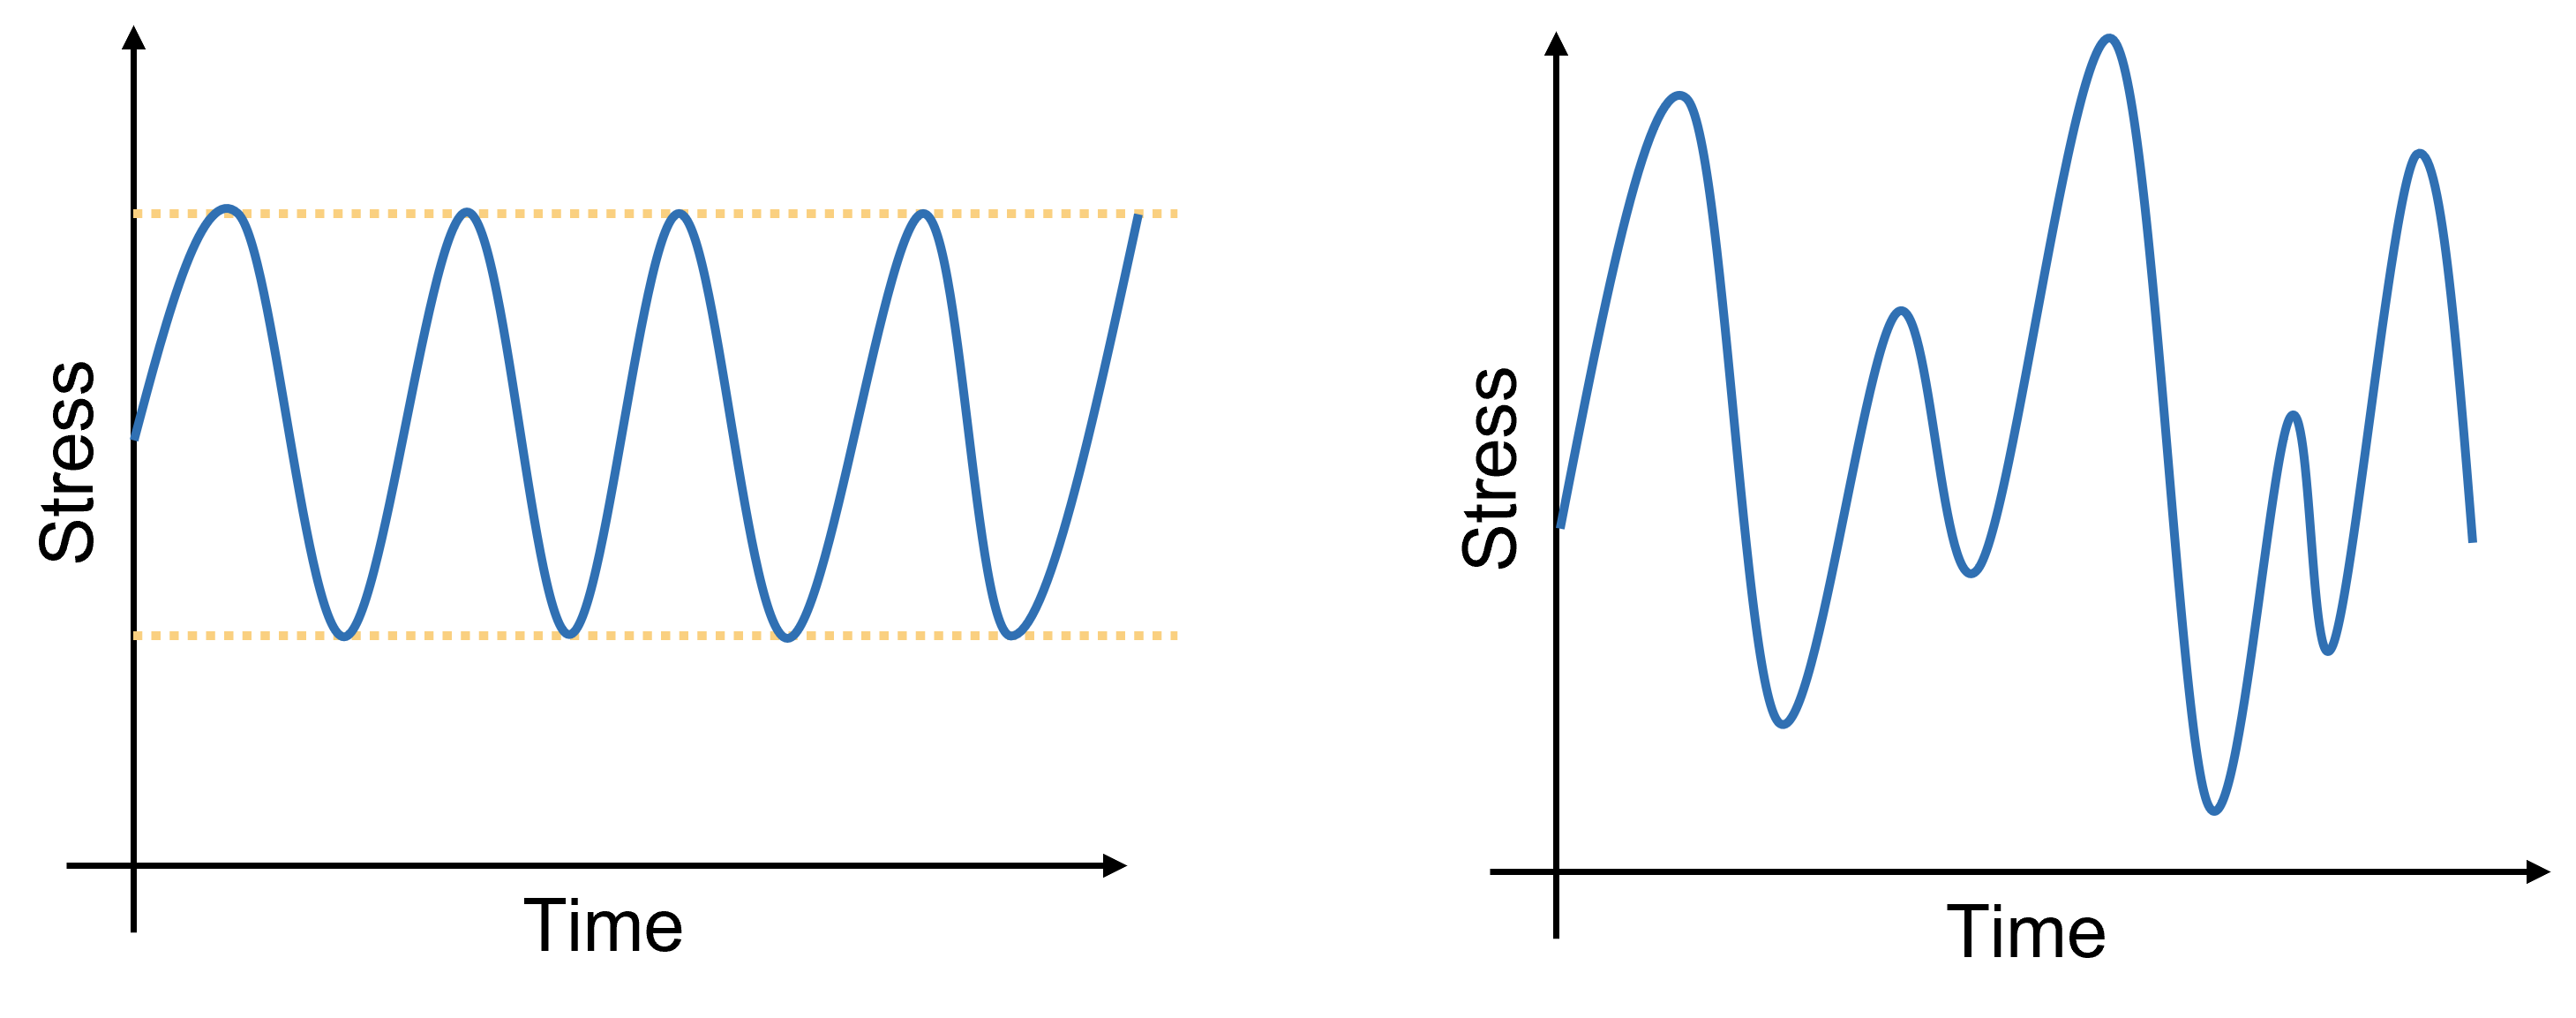
\includegraphics[width=0.8\linewidth]{IMGs/loading.png}
	\caption{Constant and variable amplitude loading}
	\label{fig:VAL}
\end{figure}
 
The Load Spectrum deals with the occurrence of load cycles with different amplitudes within a load sequence \cite{Facchinetti}. To get a load spectrum from a load sequence, the time and order component are omitted. A load spectrum shows the number of occurrences of a certain load amplitude in a load sequence.
By eliminating the order and time component of a sequence, the same load spectrum may arise from multiple different sequences. Depending on the desired detail in the load spectrum, the load levels of a sequence can also be rounded. Depending on the area of application, the rounding can be done to the next integer or the next 10,000.

The rounding will increase the occurrences at a certain load level as more occurrences are projected in each category. 
Figure \ref{fig:LS} shows a schematic load spectrum calculated from an exemplary load sequence.


\begin{figure}[H]
	\centering
	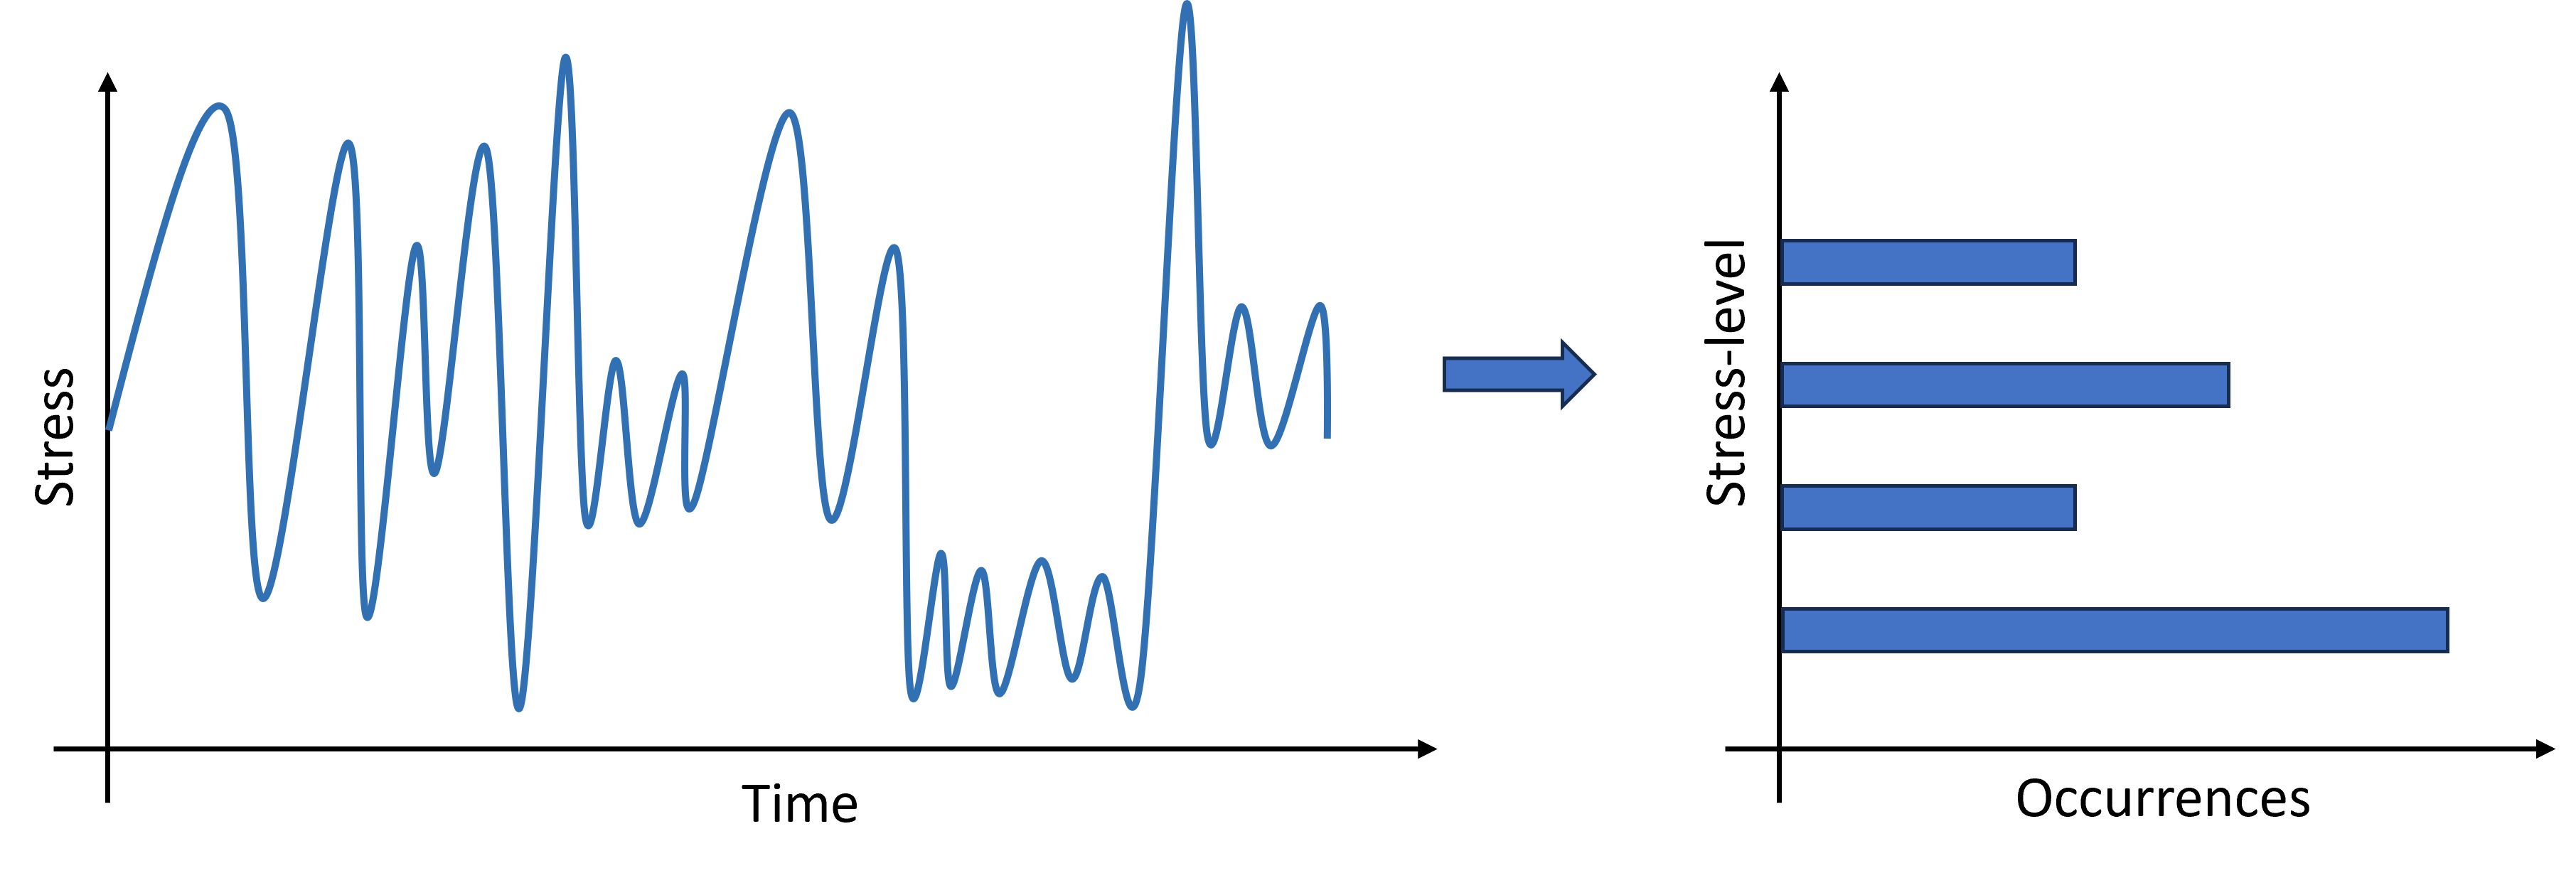
\includegraphics[width=0.95\linewidth]{IMGs/Spectrum.png}
	\caption{Load Spectrum from Load Sequence}
	\label{fig:LS}
\end{figure}

\subsection{The S-N Curve}\label{sn}
The S-N curve (also referred to as the Wöhler-curve) plays a very important role in fatigue analysis. It is applied in all aspects of engineering \cite{Burhan,Pungo}. 
The graphical representation gives clear insights into the maximum number of load cycles a material is capable of withstanding before a fatigue break is expected.
The applied load (S) is placed on the \(y\)-axes and the number of cycles (N) on the \(x\)-axes. The curve shows the number of cycles to fatigue failure and is individual for every material and for every different component.
The S-N curve can also be determined for elements like welded joints or whole structures \cite{Baptista, Dong}.
Both axes are on a logarithmic scale to achieve a straight line passing from the upper left to the lower right of the graph \cite{Little}.

Figure \ref{fig:WO} shows a schematic representation of the S-N curve: 

\begin{figure}[H]
	\centering
	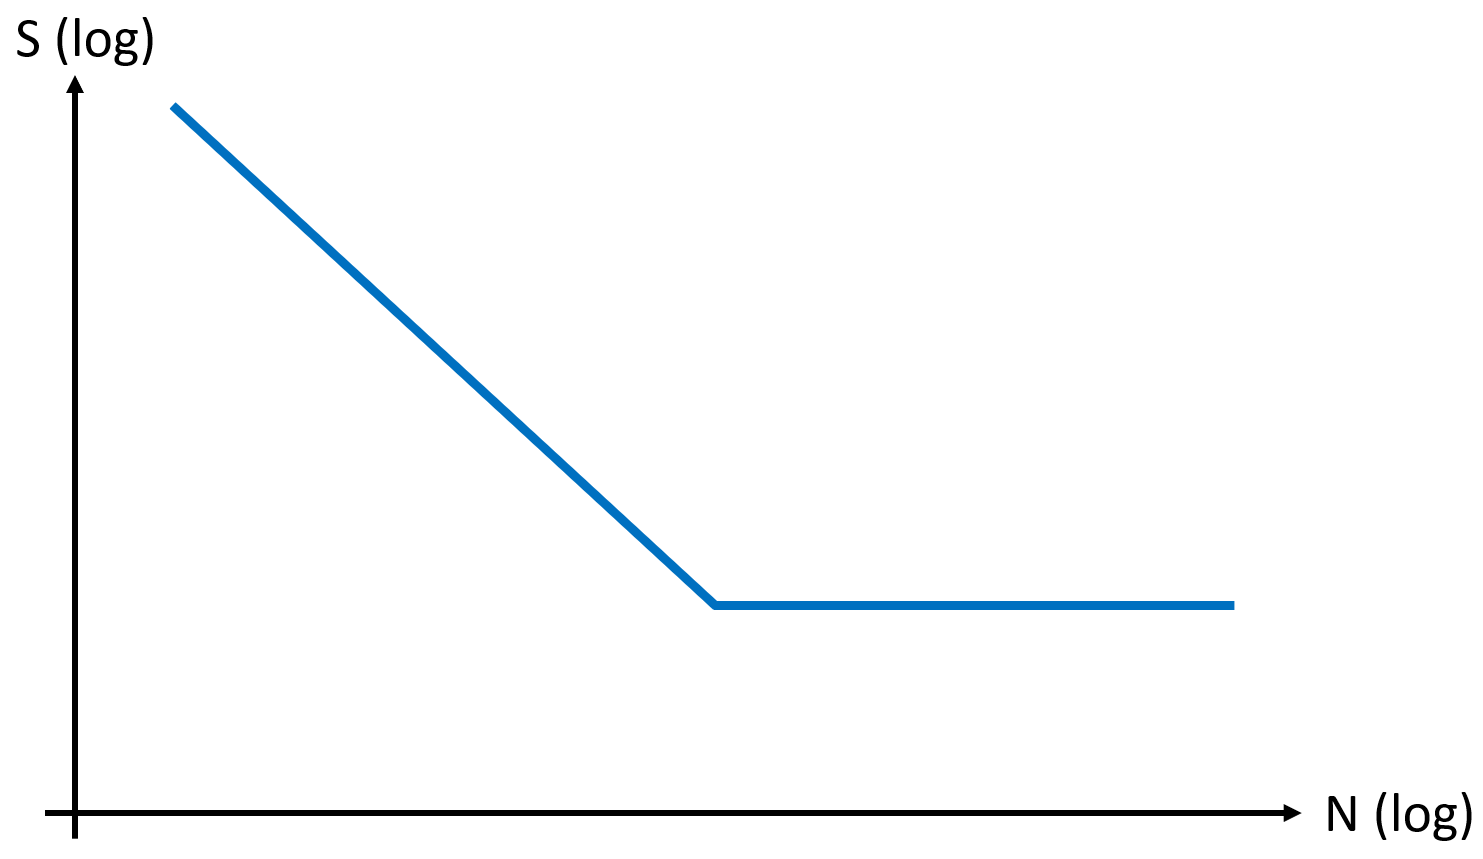
\includegraphics[width=0.7\linewidth]{IMGs/WO.png}
	\caption{Schematic representation of a S-N curve}
	\label{fig:WO}
\end{figure}
\newpage
As can be seen in figure \ref{fig:WO}, the curve is made up of two straight lines. The first part, which has a negative slope, is referred to as a fatigue strength range. In that range of loads, the material shows a limited number of cycles before failure occurs \cite{Adasooriya}.

The horizontal line marks the endurance limit, also known as the fatigue limit. Below that load level, it is assumed that a material can withstand an infinite number of cycles without failure \cite{Bellows}. It is often denoted as the S-N curve plateau.
It is important to note that the S-N curve is determined by experiments conducted in controlled environments and not on real-life machinery in industrial applications. Real-world applications may involve additional factors, such as varying load levels, environmental conditions, and surface finishes, which can influence fatigue performance \cite{JanOveHolmen}. 

Figure \ref{fig:WO2} gives a clear insight on how the S-N curve is actually a probability distribution and not a fixed deterministic line. This distribution arises from the different number of cycles achieved in experiments at the same stress level before failure occurred. Depending on the component and material, is not necessarily a Gaussian distribution. 

\begin{figure}[H]
	\centering
	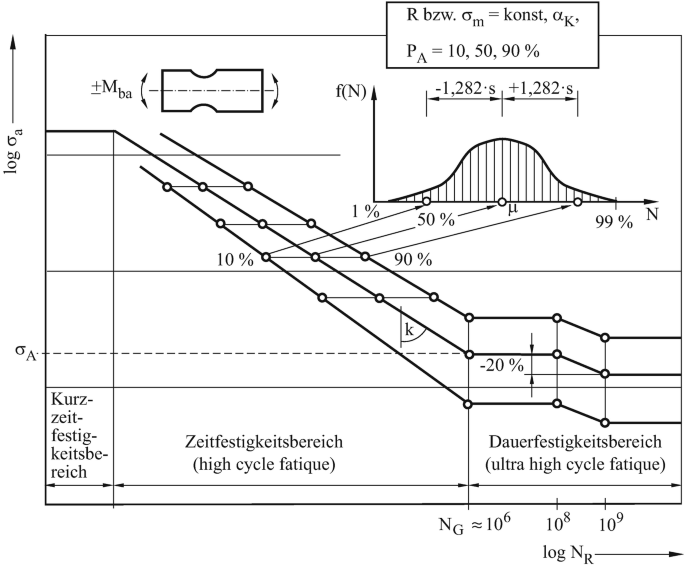
\includegraphics[width=0.7\linewidth]{IMGs/WO2.png}
	\caption{S-N as a distribution \cite{Klein}}
	\label{fig:WO2}
\end{figure}
\newpage
\subsection{Linear Damage Accumulation Method}\label{LAD}
The S-N curve is a crucial component in the application of the Miner rule \cite{MinerOG, Subramanyan}. The Miner rule is a popular linear damage accumulation technique most commonly used in engineering. It is based on three assumptions. First, that the rate of damage accumulation is constant over each loading cycle of one load level. Second, damage only occurs if the applied stress is higher than the fatigue limit (S-N curve plateau). This assumption is only true for the Miner-original and not for Miner-elementar or Miner-Haibach \cite{Werner}. And third, the component is expected to fail when cumulative damage reaches the unity \cite{Zuo}.
The Miner rule also assumes that the first load cycle at a certain stress-level is just as damaging as any other at that stress-level. The order of loads is not relevant when calculating the accumulated damage.

Each load-cycle damages the machine element inversely proportionate to the number of maximum loads the component could withstand at that stress-level. For example, if a component is capable of withstanding 1,000 loads at a certain stress level, one of those cycles adds 1/1000 to the accumulated damage of the machine element.
If another component can withstand 50 cycles at a different stress-level, each of those cycles adds 1/50 to the accumulated damage.

For varying loads, the sum of those individual ratios forms the accumulated damage. 
For example, 25 percent of the fatigue life is used up if a part is repeatedly loaded for 500 cycles at a stress level that would lead to failure in 4,000 cycles and then followed by 2,000 cycles at a stress level that would lead to failure in 16,000 cycles.
Equation \ref{acc} is how the accumulated damage-sum D is calculated. At stress-level \(S_1\), \(S_2\) ... \(S_i\), the corresponding numbers of load are \(n_1\), \(n_2\) ... \(n_i\). The number of cycles to failure under each stress level are \(N_1\), \(N_2\) ... \(N_i\).

\begin{equation}\label{acc}
	D = \sum_{j=1}^{k}\frac{n_i}{N_i}
\end{equation}

As mentioned before in chapter \ref{sn}, the individual points \(N_i\) in the fatigue strength range are determined by applying one load in a cyclic manner, to determine the maximum acceptable cycles. When using this number as a ground truth in the Miner rule, the effects of other loads, happening before or after, are neglected. To solve this, non-linear damage accumulation methods were developed.

\subsection{Non-Linear Damage Accumulation Methods}
One of the first non-linear fatigue damage accumulation models was the expansion of miner rule by a power law \cite{Zuo}.
Equation \ref{n1} shows how the damage sum D is calculated. The parameter \(C_i\) is a material parameter corresponding to the i-th loading level. 

\begin{equation}\label{n1}
	D = \sum_{j=1}^{k}\left [\frac{n_i}{N_i}\right ]^{{C_i}}
\end{equation}

The disadvantage of this method is that the parameter \(C_i\) must be calculated for different loading
conditions and thus tedious to acquire \cite{Zuo}.

Another approach, used in \cite{Rege}, proposes to use iso-damage-curves as a basis to calculate the cumulative fatigue damage.\newline
Many more approaches can be found in \cite{Zhu1,Gao,Lv,Chen}.

The common disadvantage of non-linear models is that they are dependent on very individual and specific parameters, limited to certain materials or loading histories, with a fixed trend regarding the loading amplitudes. Due to those limitations and cumbersome usage, they are not widely adopted in the engineering field \cite{Vietze}. 


\newpage
\section{Overview of Machine Learning}
In contrast to rigid algorithms, ML is a method that can solve a given problem without being explicitly told how to solve it \cite{Sutton,Janiesch}. The following chapter discusses the advantages, general functionality, and core principles of ML.

\subsection{General Introduction to Machine Learning}\label{General Introduction to Machine Learning}
ML is a subsection of the field of general AI \cite{Helm}. The same as deep learning (DL) is a subsection of ML \cite{LeCun}.
AI encompasses the general principles and methods that can mimic human behavior and decision-making \cite{Janiesch}. ML, on the other hand, incorporates all methods that can learn from data and discover regularity and patterns that are not obvious to a human~\cite{Theodoridis}. Based on the discovered knowledge, the trained model can be used to make predictions for new inputs in the future.
DL is a subset of ML that refers to methods that utilize a special approach called a Neural Network (NN). The "depth" in DL in this context refers to the amount of stacked layers of neurons (see chapter \ref{NN chapter}) \cite{Carleo}. 
DL is more capable than shallow ML and shows improved learning capabilities, but it also comes with its own specific challenges \cite{Janiesch, LeCun}.

Figure \ref{fig:AIMLDL} shows how DL and ML are subsets of AI. 

\begin{figure}[H]
	\centering
	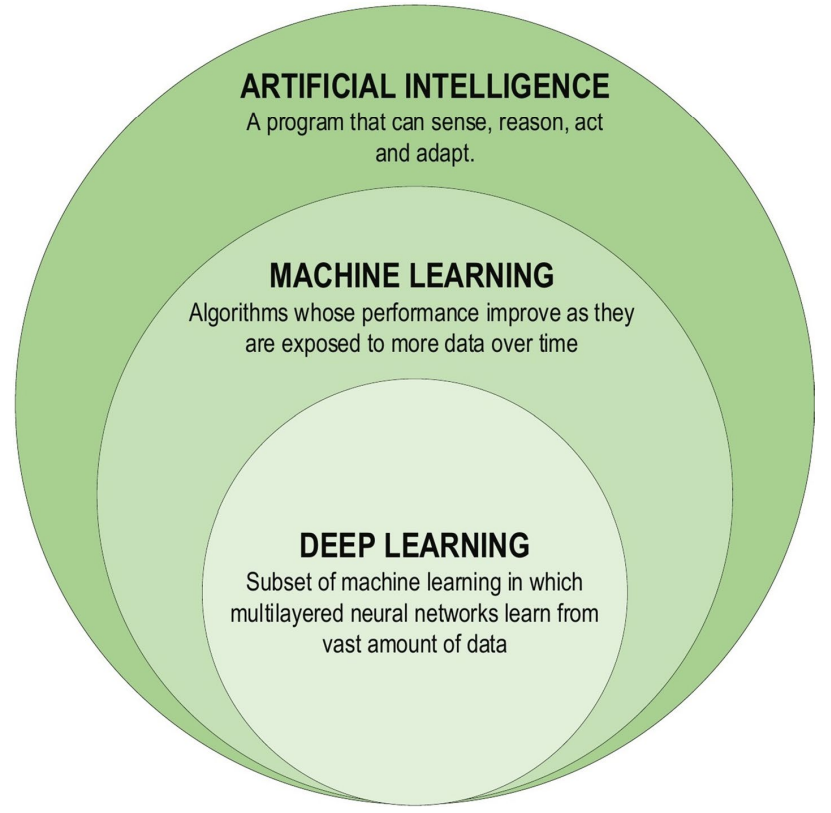
\includegraphics[width=0.7\linewidth]{IMGs/AIMLDL.png}
	\caption{Venn-Diagram of the different subsets of AI \cite{Alzubaidi}}
	\label{fig:AIMLDL}
\end{figure}
\newpage
\subsection{Advantages and Problems of Machine Learning}\label{Advantages and Problems of Machine Learning}
The most important \textbf{advantage} of ML is the ability to learn from data and discover the underlying, non-obvious patterns \cite{Wuest}. With that knowledge, it is also possible to predict the output for a specific input. A ML model deployed to a self-driving car could, for example, predict how a pedestrian is going to cross a street and calculate if the car should perform an emergency brake to avoid a collision. One further advantage of ML is its wide applicability \cite{Thommandru}. Not only computer science or the automotive industry, but also banking, healthcare, and many more fields, can all find applications where ML can help improve a process.

These algorithms are also very efficient and profit greatly from more available data \cite{Janiesch}. Not only is it possible to learn from a lot of data, but also to process a lot of data \cite{Wuest}. One example is the analysis of sensor data, for example, from LiDAR sensors. Those sensors produce a lot of data that might need to be analyzed as quickly as possible, in some cases even in real-time. For self-driving cars, fast analysis of this data is crucial for avoiding accidents. ML is capable of solving this problem reliably \cite{Lyu}. 

The era of "Big Data" plays right into the hands of ML. More data results in better performance of the ML approaches \cite{Wuest}. Also, the methods can be specially adapted to be robust. Outliers, noise, and missing values in the data do not skew the results in a significant way \cite{Theodoridis}. When comparing ML to DL, ML can tend to produce better results in cases where the training data is limited and also allows for a better interpretation of the outputs of the model \cite{Janiesch}.

The \textbf{disadvantages} of ML are closely related to the advantages. For example, the data-set that is used for training needs to be a certain minimum size so the model is able to learn the underlying patterns. But not only the size is important, but also the contained elements, as some models can return different results based on the elements that make up the data-set. The effectiveness of ML rises and falls with the amount and quality of the data \cite{Janiesch, Bishop}.

One of the biggest problems of ML is generalization \cite{Bishop}. Finding and learning patterns is just the first step, but making a correct prediction is the most valuable part. Depending on the free parameters of ML models, they have the capability to memorize the whole presented training-set and perform very poorly on data that is not part of the training-set \cite{Zhangpiml}. This case is called "over-fitting" \cite{Jabbar}. In such cases, the model does not learn the underlying structure of that data, but just the correct associations from one input to one output. 

The opposite of "over-fitting" is called "under-fitting" \cite{Jabbar}. The model is not capable of learning any patterns, and thus performs very badly on the training set and on newly presented test samples. This happens mostly when the data-set is not large enough for the chosen model or the model is not flexible enough to adapt to the pattern of the data \cite{Will}. In a worst-case scenario, a ML method could interpret the noise of the data as a pattern, and perform very poorly when applied in real-world applications.\newline

Especially for high-dimensional data and complex problems, a very large dateset is a must. This can be difficult to obtain, especially in the area of natural sciences or industry \cite{Wuest}. Sensors can provide very corrupt data, and some experiments can take a lot of time and money to perform. And if that data is acquired, it still requires a significant amount of manual work to bring it into a form where ML methods can work with it. To train a model, for example, to classify multiple bacteria cells, it first takes time to grow the bacteria, but then also to label all the pictures. For example, the MNIST data-set for number recognition contains 70,000 elements, that were all manually labeled \cite{Pavlo}. So depending on the area or application, it is impossible to obtain a data-set that has the necessary size and quality. 

Further, models can be very susceptible to hyperparameters \cite{Janiesch}. Hyperparameters are fixed values that describe the characteristics of a model. Those values are set manually and require extensive knowledge about the implemented model, the problem at hand, and the available data-set \cite{Luo}. The optimal parameters can be found with an extensive brute force approach or specialized algorithms, but they require too much time to be feasible in an industry-application~\cite{Claesen}. 

Table \ref{AdDis} summarizes the advantages and disadvantages of ML. Despite its disadvantages, the abilities and unique advantages of ML make it a very interesting addition to industry applications~\cite{Bertolini}. Especially as more and more capable methods are developed. The main goal when implementing ML is to work around the disadvantages to achieve the desired results.


\begin{table}
	\begin{center}
	\begin{tabular}{|| c | c ||}
		\hline
		\rule{0pt}{2ex}
		 Advantages of ML & Disadvantages of ML \\
		\hline
				\rule{0pt}{2ex} 
		$\bullet$ can learn from data & $\bullet$ requires large datasets \\
		$\bullet$ can make predictions based on learned patterns & $\bullet$ data is tedious to acquire\\	
		$\bullet$ versatile in applicability & $\bullet$ is sensitive to hyperparameters\\
		$\bullet$ can process a lot of data efficiently & $\bullet$ can be sensitive to training-set\\
		$\bullet$ can handle noise and outliers in data & $\bullet$ over-fitting / under-fitting\\
		\hline
	\end{tabular}
	\caption{Advantages and Disadvantages of ML}
	\label{AdDis}
\end{center}
\vspace{-4mm}
\end{table}
\newpage
\subsection{General Terms in Machine Learning}
In the following, some of the general terms in ML are explained. As the field of ML is very large and continuously growing, this section focuses only on the core elements. Understanding these terms and principles helps to get a better understanding of the ML methods and how they can be applied in industry. For a more in-depth look, more information can be found in extensive literature \cite{Theodoridis, Bishop, google}.

\subsubsection*{Training and Testing}\label{TT}
To train and test the model's ability to generalize, the data is split up into a training-set and a test-set. The training-set is used to determine the optimal parameters of the model \cite{Bishop}. The process of finding the optimal parameters is referred to as training or learning. It is important to keep both sets separate and only use them for their respective purposes. The training-set must not contain elements of the test-set and vice versa. Otherwise, if the expected error is computed on the training-set, the ability of the model to generalize is not correctly assessed \cite{Xiaogang}.

One easy way to understand the search for optimal parameters during training is with the example of curve-fitting of a polynomial function (see \cite{Bishop} for a more in-depth look). \newline
Function \ref{fun1} is a polynomial of degree \(M\) with free parameters \(w_i\) that can be adapted to fit the data as accurately as possible.
The error function, defined in equation \ref{err1}, also called loss function, measures the accuracy of the polynomial. The parameters are changed in such a way to reduce the error. If the polynomial is flexible enough, the error is reduced to zero. In the case of ten free parameters and ten data points (\(x_n\),\(t_n\)) the polynomial passes through every data point exactly. The error in that case is zero. 
\begin{equation}\label{fun1}
	y(x,w) = \sum_{j=0}^{M}w_ij^j= w_0+w_1*x^1+w_2*x^2+...+w_M*x^M
\end{equation}
\begin{equation}\label{err1}
	E(w) = \frac{1}{2}\sum_{n=0}^{N}\{y(x_n,w)-t_n\}^2
\end{equation}

Figure \ref{fig:poly} shows how the polynomial changes based on the number of free parameters. When the polynomial, displayed in red, reaches degree nine, the error is zero. In this case, however, it is not following the true data generation function shown in green and performs very poorly on new unseen data points (see "over-fitting" in chapter \ref{Advantages and Problems of Machine Learning}).
%from \cite{Bishop}
\begin{figure}[H]
	\centering
	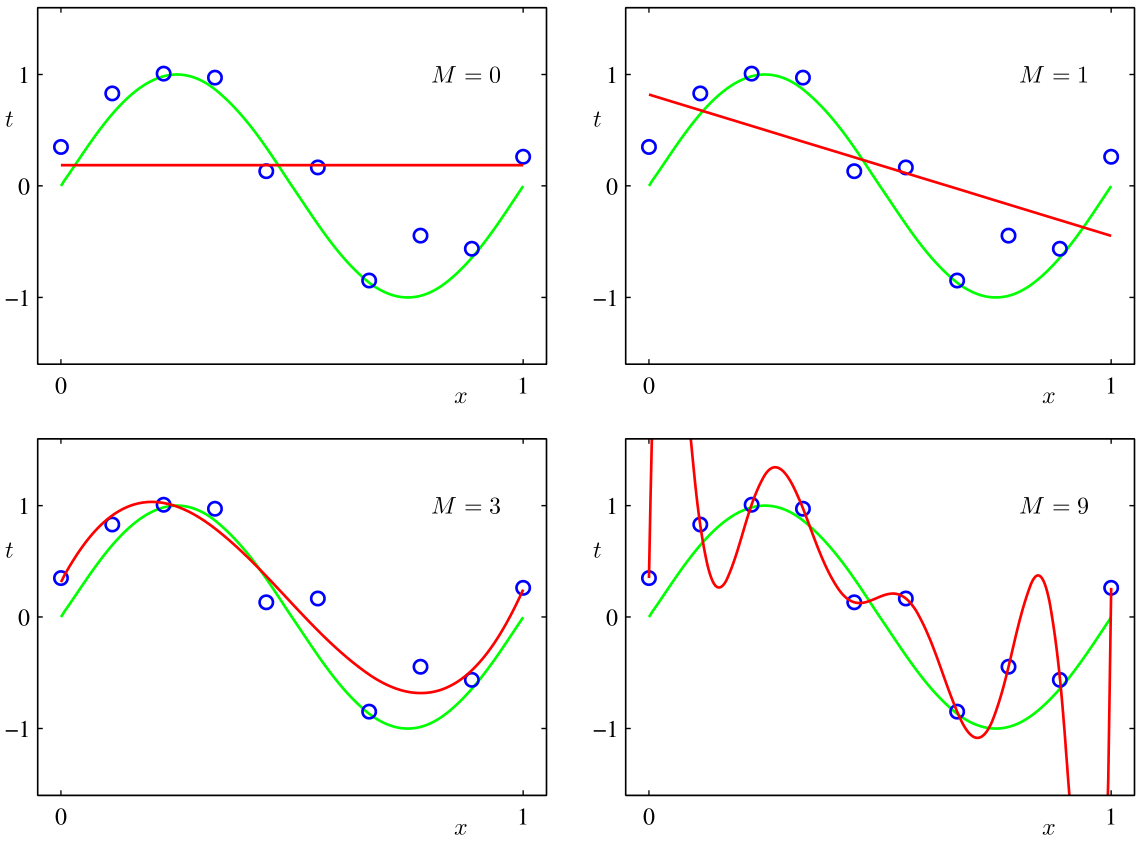
\includegraphics[width=0.8\linewidth]{IMGs/poly.png}
	\caption{Influence of the number of free parameters in curve-fitting \cite{Bishop}}
	\label{fig:poly}
\end{figure}

\subsubsection*{Features and Feature Selection}
Every model needs an input and a corresponding output. As computers work on a digital principle, physical values have to be transformed into a digital format. For example, sensor data from analog pressure valves or analog current meters has to be transformed into digital values.\newline "Industrie 4.0" did a lot of work to replace standalone analog sensors with sensors having a digital output or wireless connection, so that this translation step is no longer a hurdle. The post-processing of those signals can be done on a central computer or dedicated edge devices on the shop floor \cite{Lu}.

But not all data is accepted by a ML model right away, even if it is in digital form. These methods need an input that is specifically shaped for each specific model.
When the goal is to apply a ML model for image classification, the image needs to be transformed into a format that is accepted by the implemented model. Images can have different height-to-width ratios (e.g.,~16:9 or 4:3) and different resolutions (e.g.,~1920x1080 pixel or 64x64 pixel). All the images need to be transformed into a uniform shape with the same resolution \cite{Park}.

For example, if an image data-set contains mostly images with a 1:1 ratio, wider images need to be contracted or cut off to fit the pattern so that all images are the same. The resolution must also be adjusted so that all images have the same number of pixels.
\newpage
Figure \ref{fig:pixel} shows how images of different sizes and resolutions are adapted to a fixed resolution and ratio. In the upper image, the overhanging parts on the sides are removed, and no resolution scaling is necessary. In the lower image, parts on the top and bottom are removed. Additionally, the resolution was downscaled from 125x125 pixel to 100x100 pixel. 

\begin{figure}[H]
	\centering
	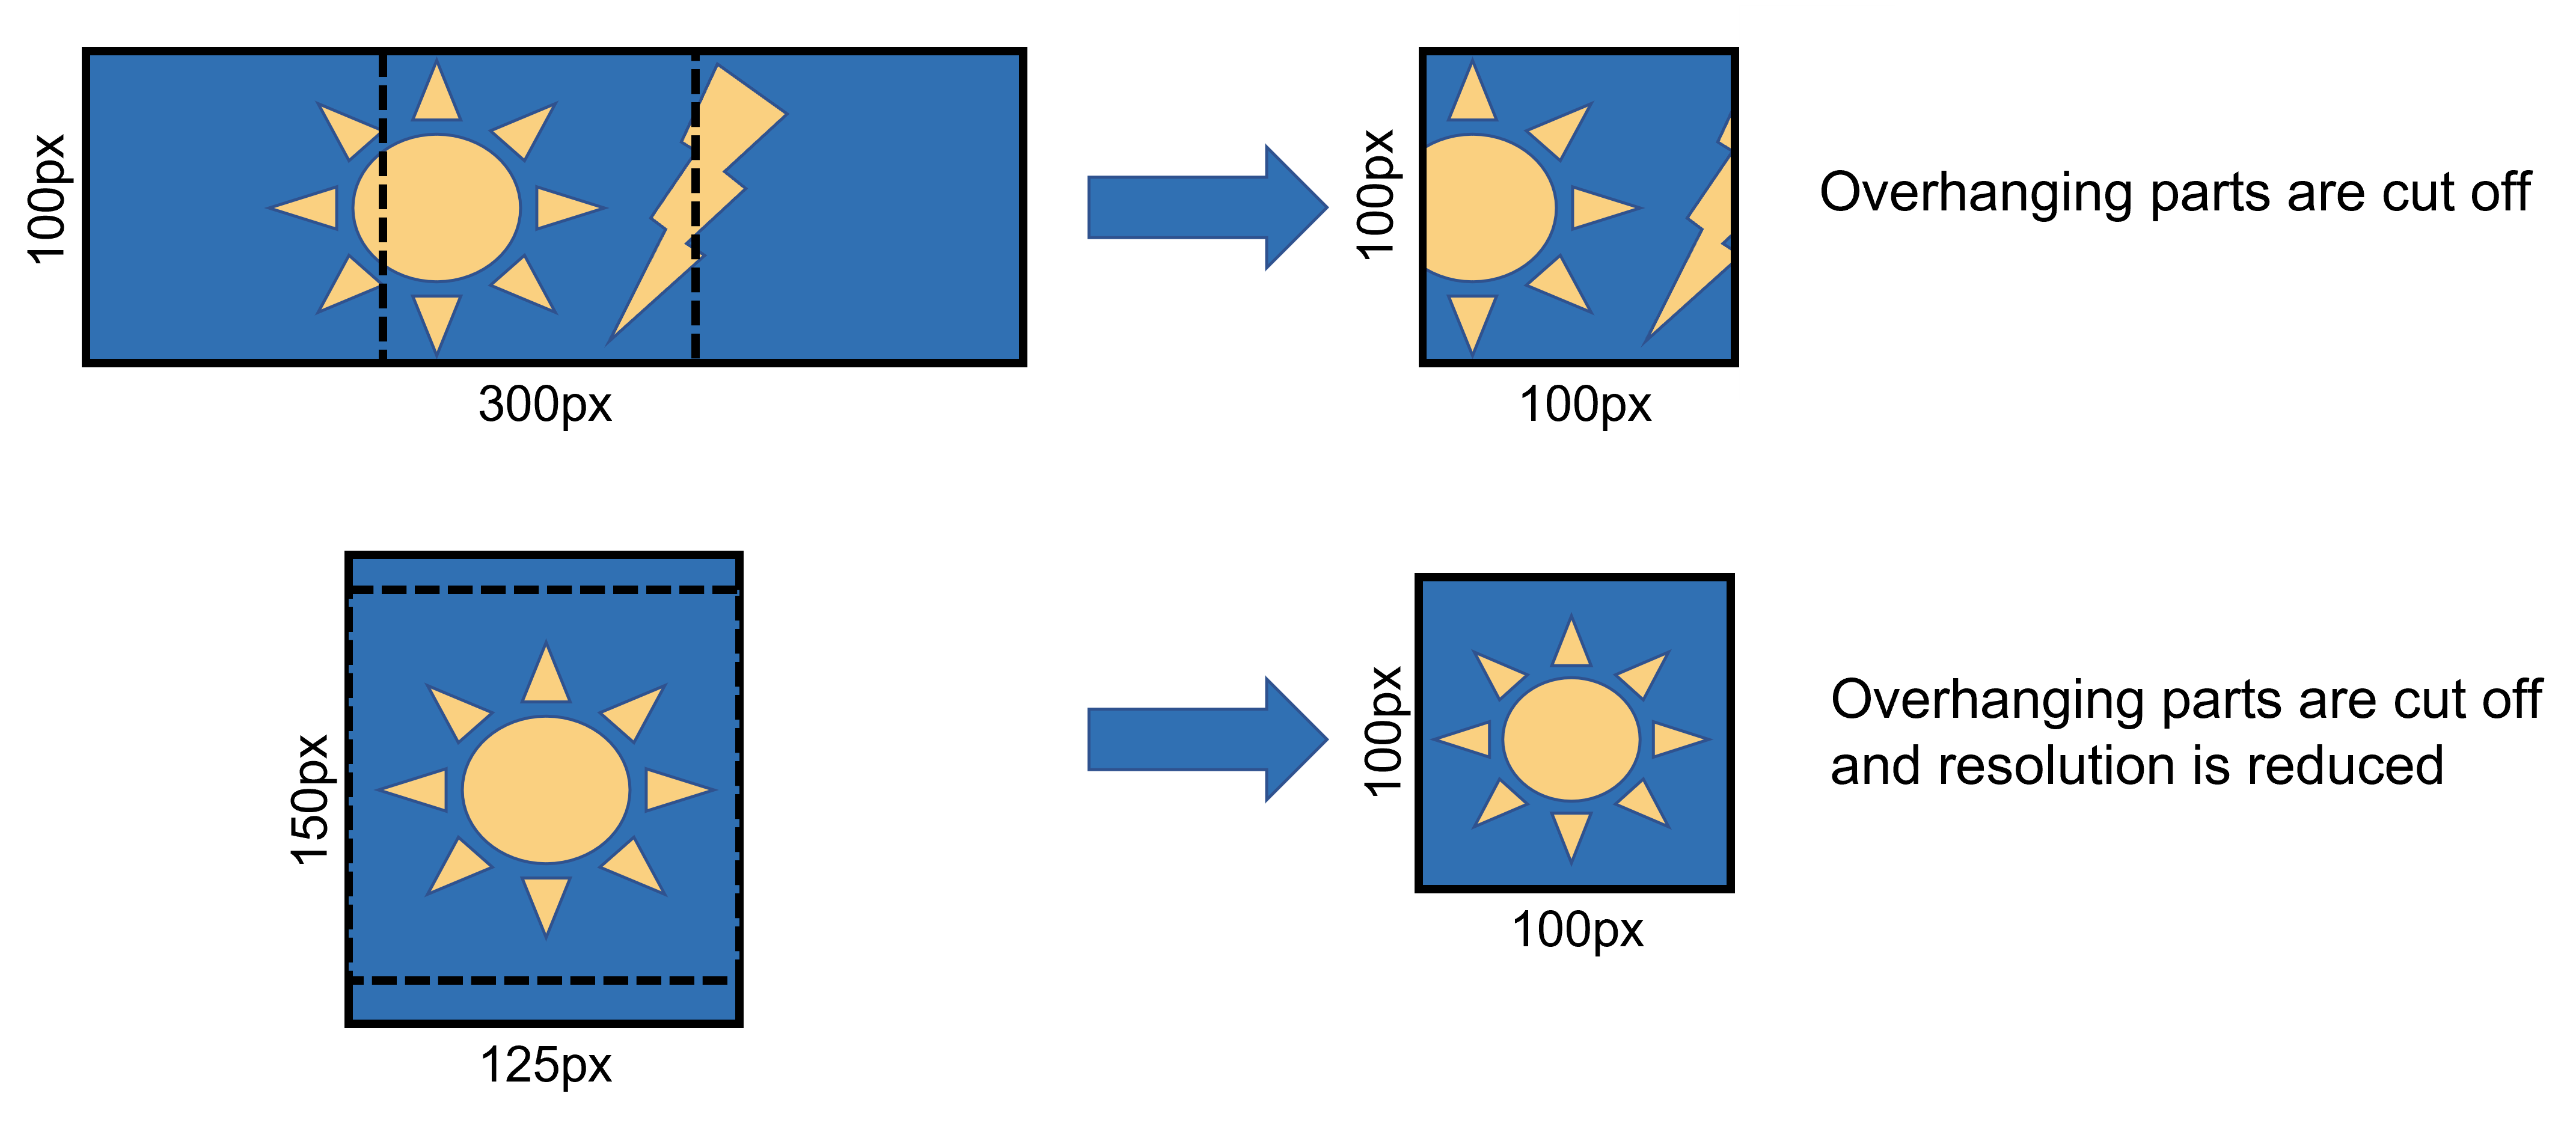
\includegraphics[width=0.95\linewidth]{IMGs/pixel.png}
	\caption{Changing resolution and ratio of images for a homogeneous data-set}
	\label{fig:pixel}
\end{figure}

The ratio and resolution depend on the implemented method and can be chosen freely. 
The current standard for images (MNIST) that are used in bench-marking of various algorithms is a squared format with a 28x28 pixel resolution \cite{Baldominos}.\newline
For optimal classification, a higher resolution proves advantageous but can require longer training times and more complex~models~\cite{Kannojia,Huang}.

After the input elements are standardized, they can be transformed into a vector or matrix format. The process of constructing such designed input from raw input is called "encoding". The result after the encoding is called a "feature vector". The elements of such a vector are referred to as features. One set of features uniquely represents the uncompressed input \cite{Theodoridis}. It is possible to reduce the feature vector through a process called "feature selection", where the feature vector is reduced even further to a smaller size that contains the gist of the raw input. By reducing the dimension, the models are capable of learning faster, but this process is running the risk of omitting valuable data in the process \cite{Janiesch}.

Figure \ref{fig:encoding} shows how a matrix, representing an image, for example, can be encoded as a vector. As long as the encoding method is constant for all input elements, the order is irrelevant. In that case, the elements can also be stacked not only row-by-row but also column-by-column.

\begin{figure}[H]
	\centering
	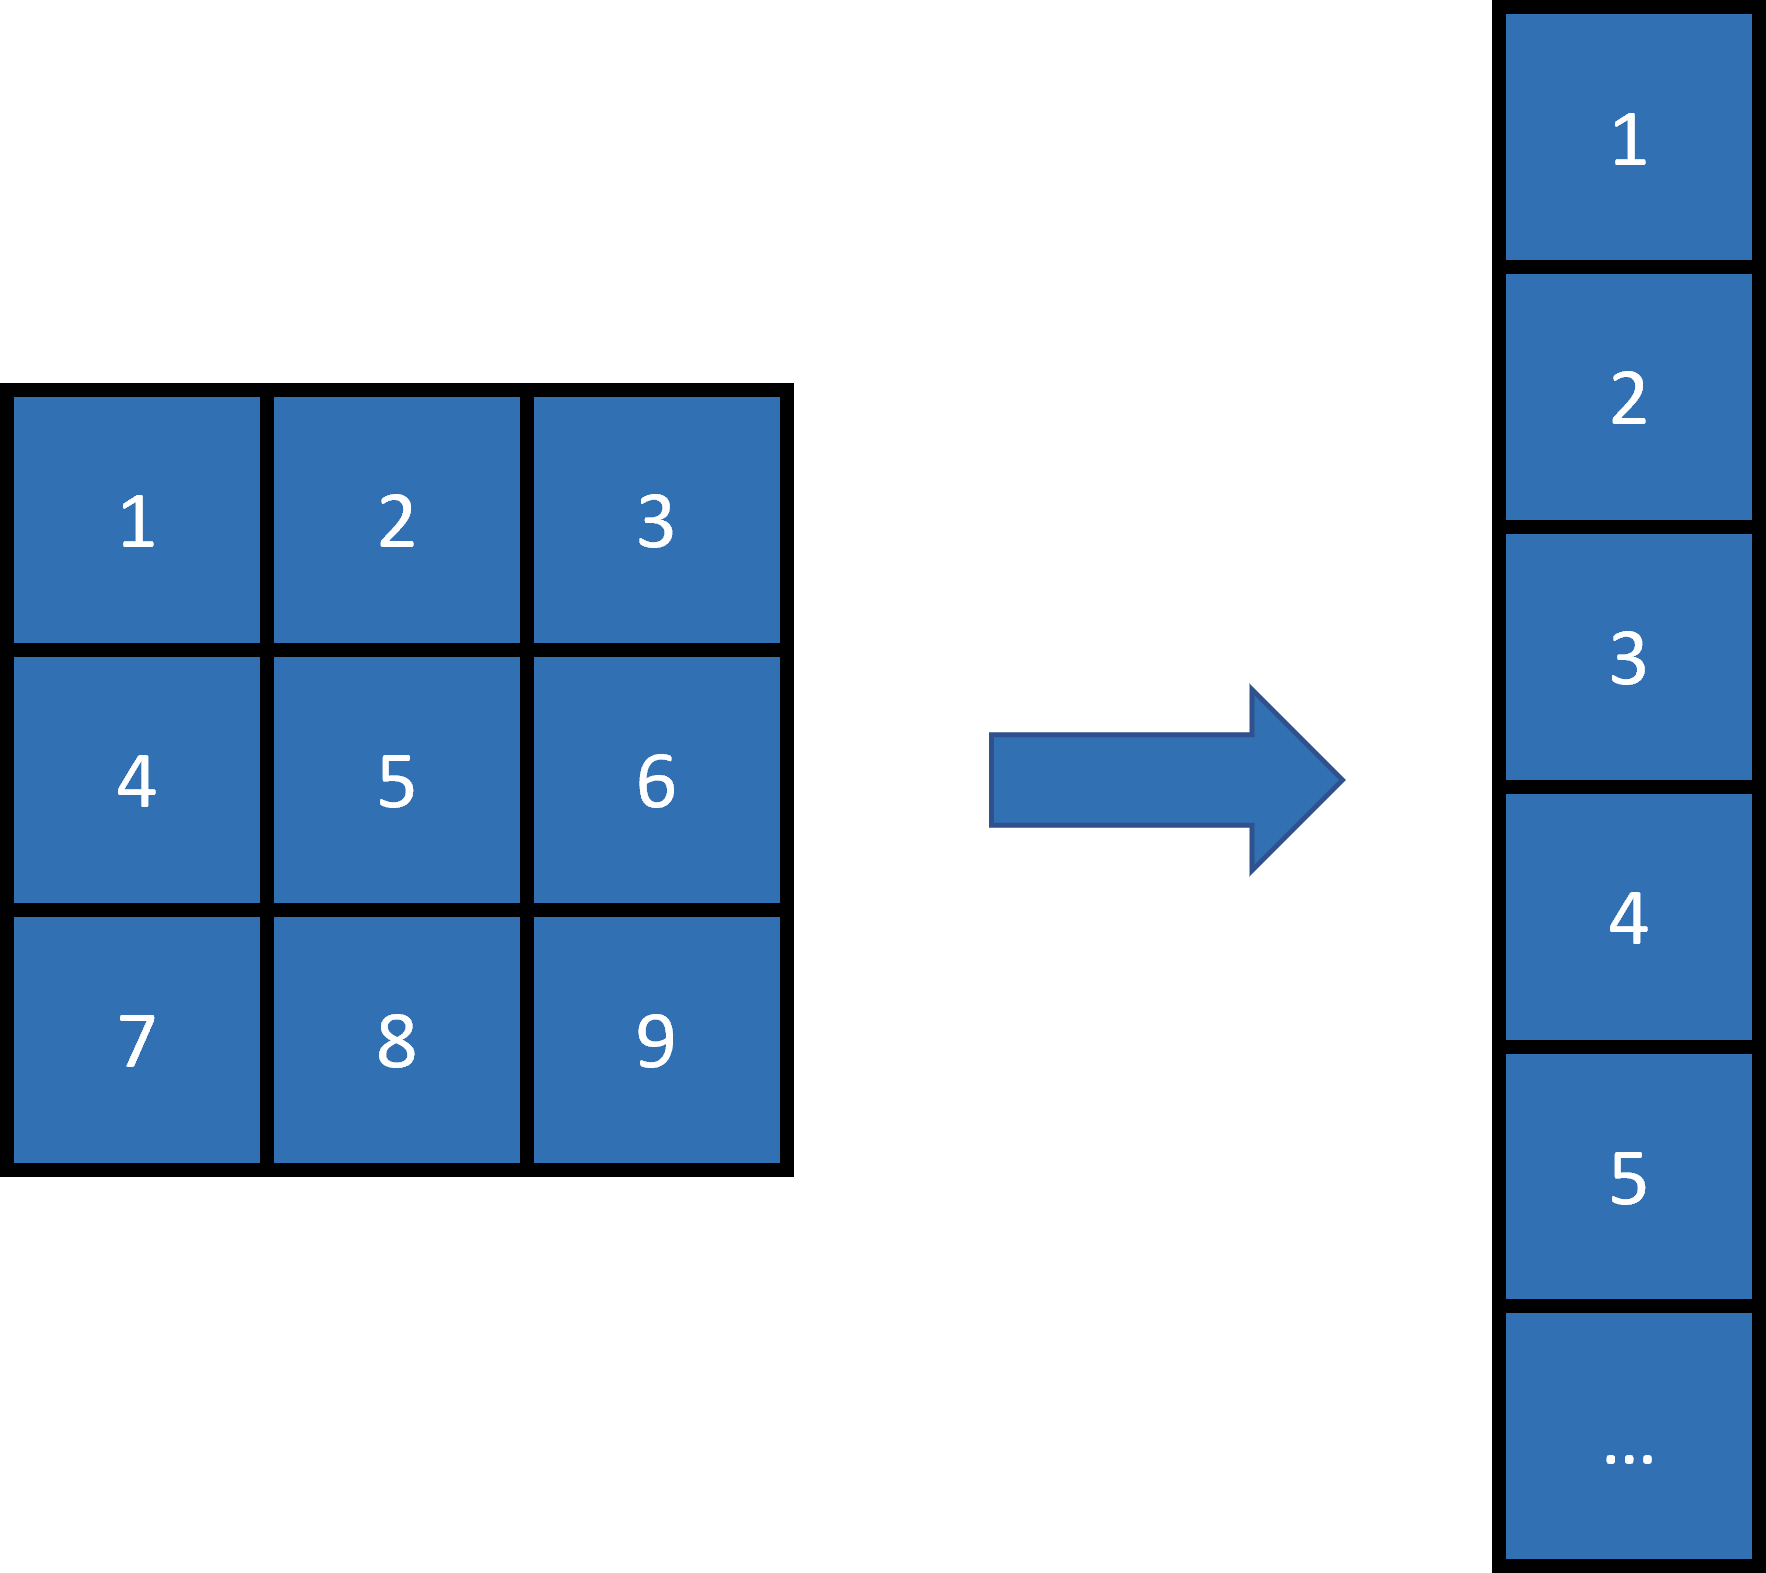
\includegraphics[width=0.455\linewidth]{IMGs/encoding.png}
	\caption{Encoding of an image-matrix as a vector}
	\label{fig:encoding}
\end{figure}

 
\subsubsection*{Data augmentation}\label{DAUG}
As mentioned in chapter \ref{Advantages and Problems of Machine Learning}, a large data-set improves the success of ML approaches. Instead of inflating a data-sets with noisy or corrupt samples and relying on the algorithm's ability to handle such data, a different approach is possible. The process of enlarging a given data-set is called Data Augmentation (DA). The goal is to bypass the problem of small datasets and increase their size and quality \cite{Shorten}. By doing so, over-fitting can be prevented. DA is mostly used on images, but can also be transferred to all other types of data. Possible DA approaches are, for example, geometric transformations like cropping, flipping, scaling, and rotating \cite{Taylor}. Further possibilities are changing the contrast, brightness, white-balance, tint of the image, as well as local pixel manipulations \cite{Mikolajczyk}. These individual adjustments can also be combined to produce a plethora of data.

Further approaches are possible when working with data in a time-series format \cite{Bandara, Wen}. One definition of time-series, is data that has a time component, like recorded sensor data, and thus can be plotted over time \cite{Hamilton}. Another definition is that the data has an orderly element and not necessarily a time component \cite{Iwana}. An example of a series without a time component are words in sentences. In such cases, cropping might distort the data too much to be representative of the original element.

One of the most straightforward approaches when working with signal data is to overlay the data with Gaussian noise or any other noise pattern. Another option is inserting or emitting repeating values of the data, which makes the time-series longer or shorter \cite{Wen}.

Figure \ref{fig:DA} shows further possible DA techniques. The different methods can be divided into basic and advanced approaches \cite{Wen}.

\begin{figure}[H]
	\centering
	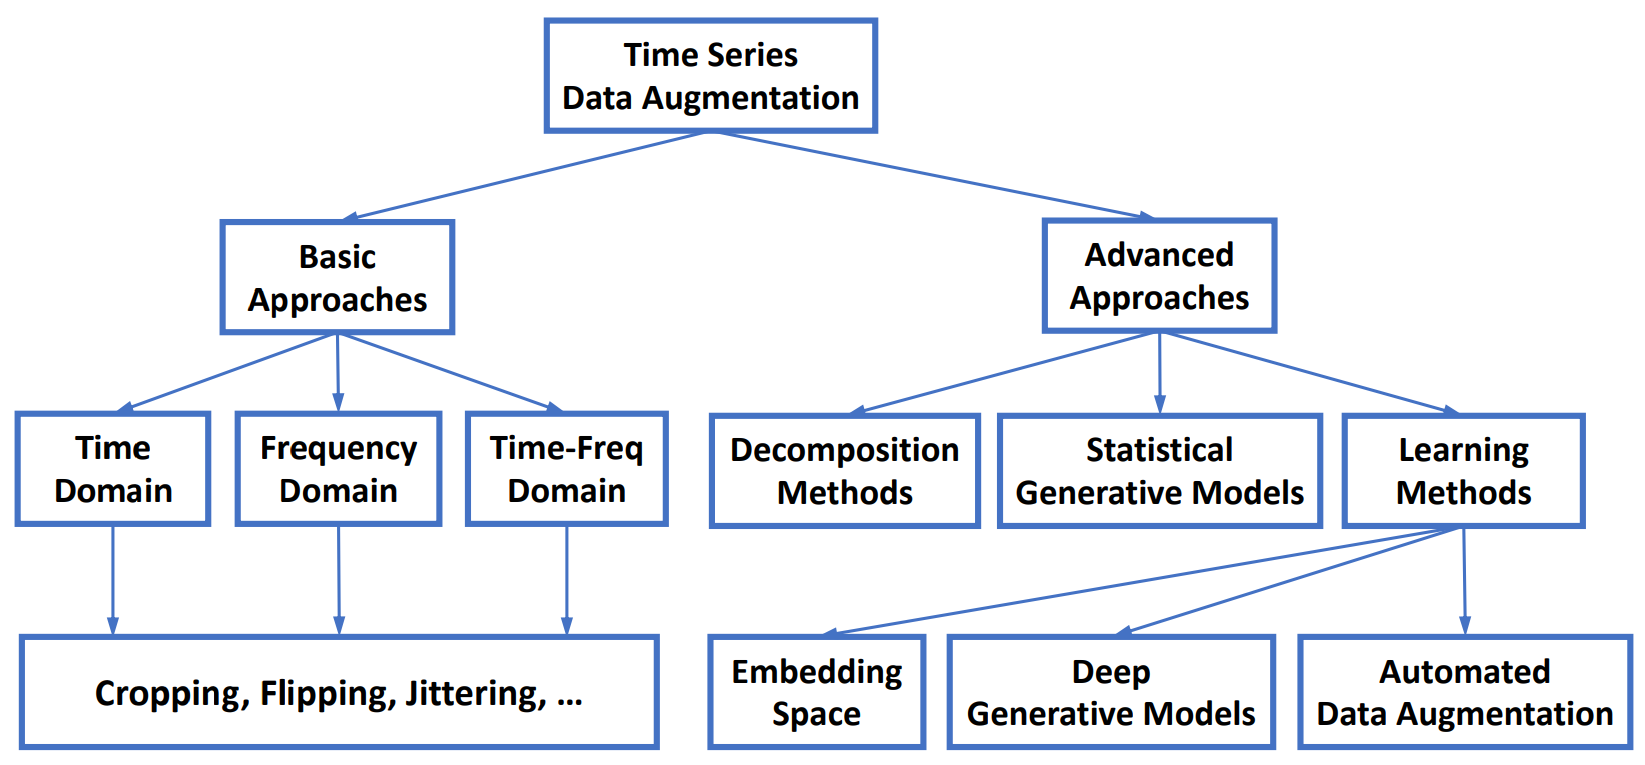
\includegraphics[width=0.9\linewidth]{IMGs/DA.png}
	\caption{Possible DA techniques for time-series data \cite{Wen}}
	\label{fig:DA}
\end{figure}

Figure \ref{fig:DA2} shows how a polynomial can be varied to increase the data-set size but still keep its significant characteristics.

\begin{figure}[H]
	\centering
	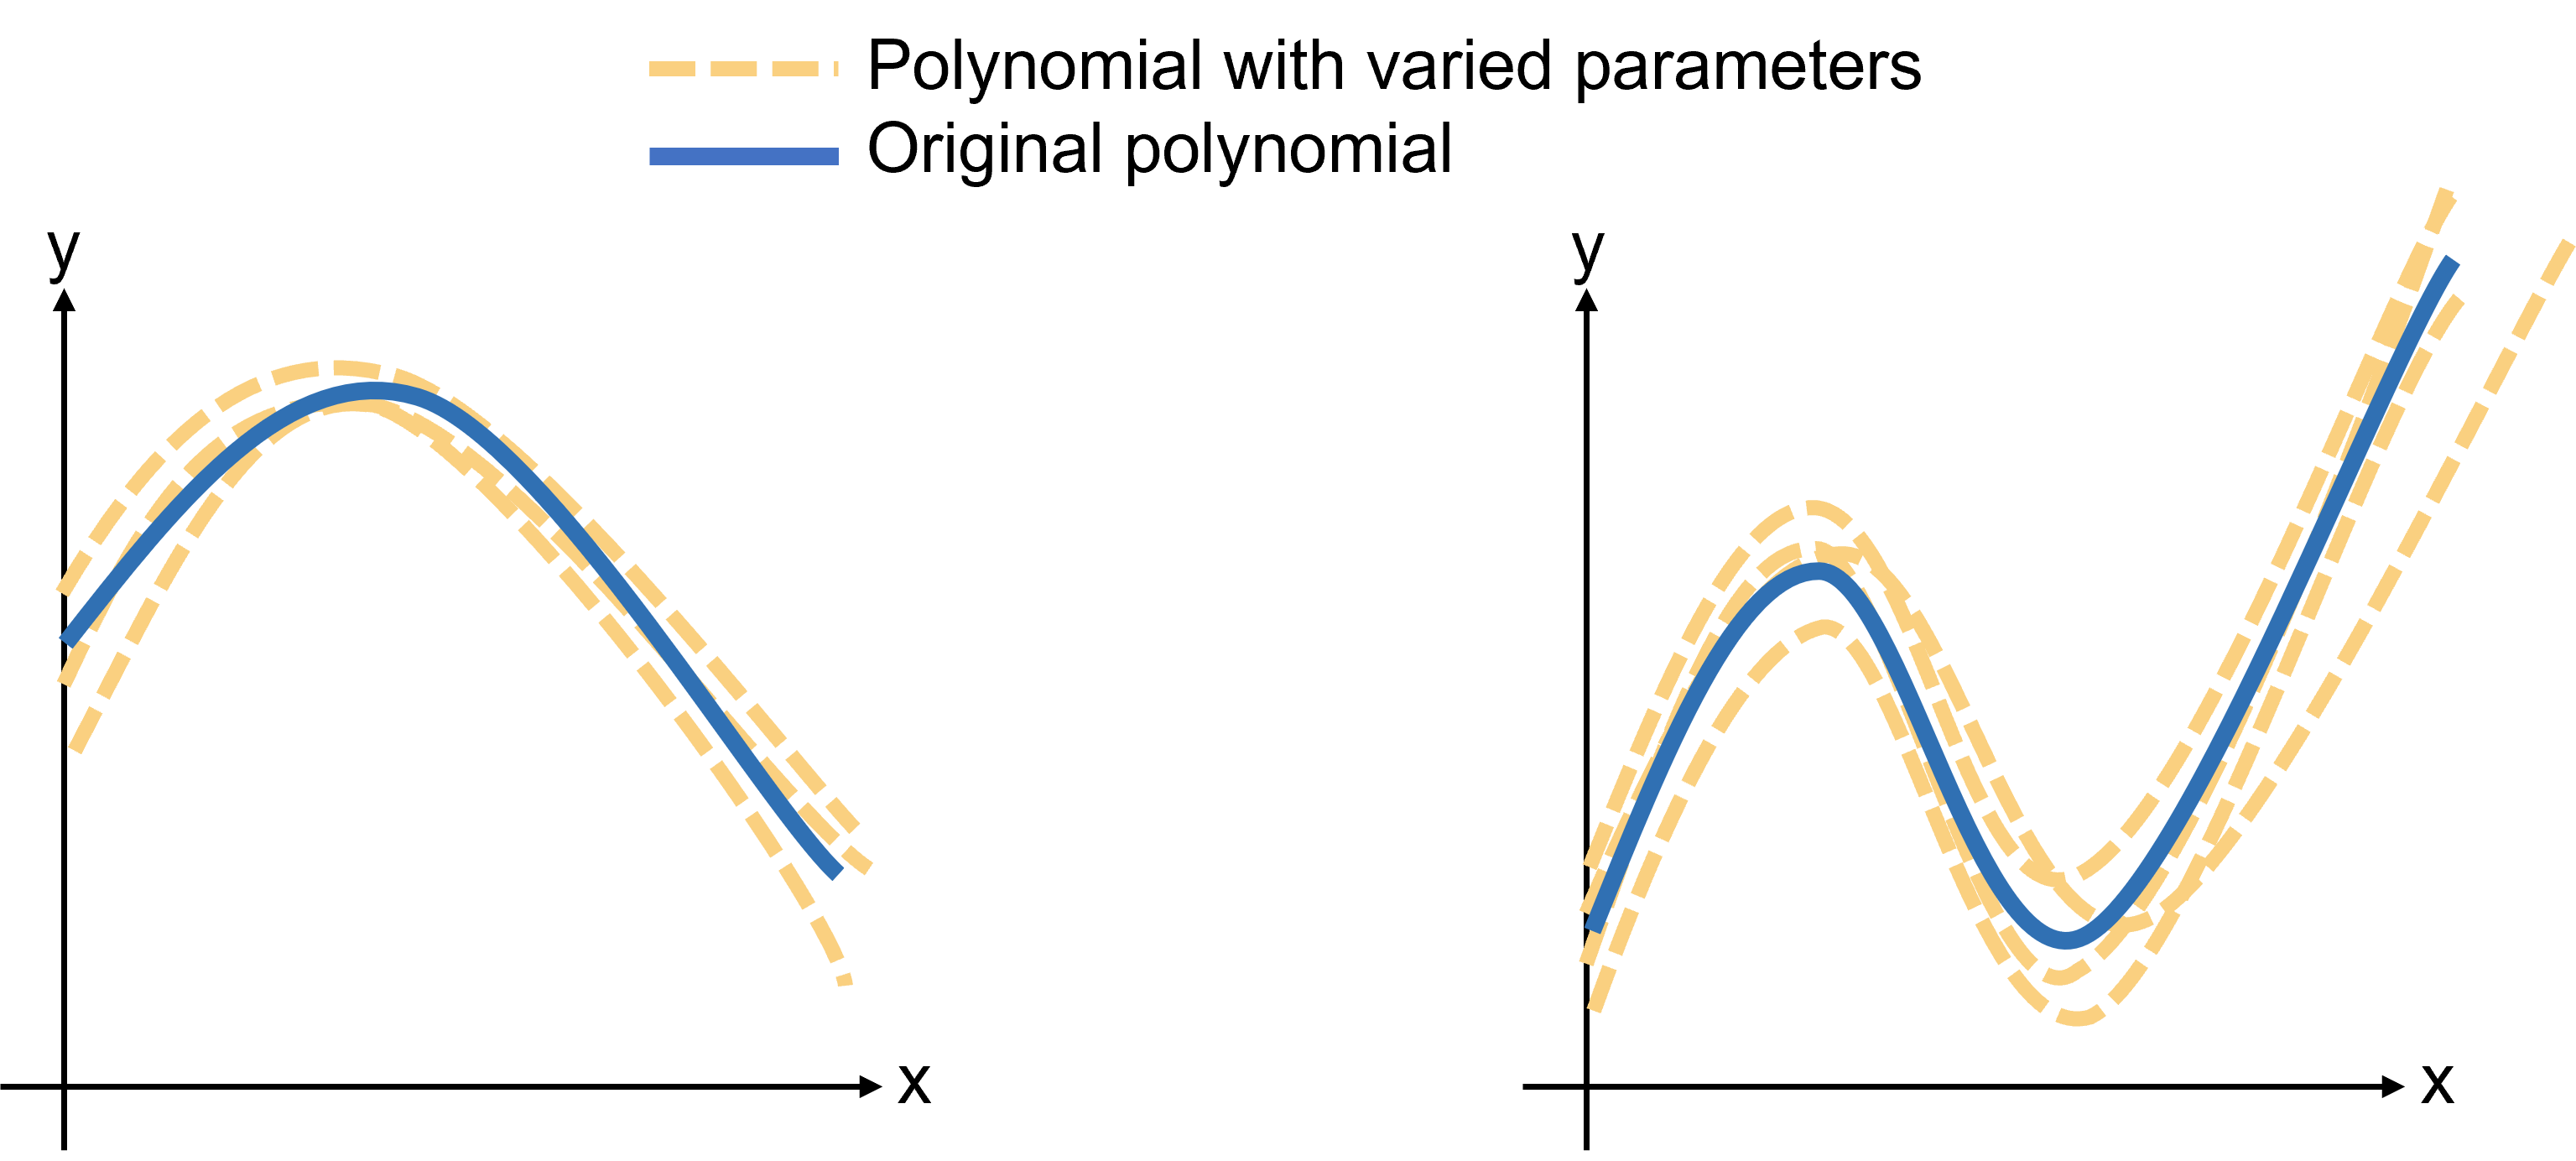
\includegraphics[width=0.8\linewidth]{IMGs/DA2.png}
	\caption{Application of DA to polynomial functions}
	\label{fig:DA2}
\end{figure}

\subsubsection*{Data Pre-Processing}
When working with a given data-set, it is helpful to the ML method if all feature vectors are in the same range across all samples.
The aim is that the greater numeric feature values are not dominating the smaller numeric feature values and each one can have an equal contribution to the output. This improves the performance of ML-methods significantly \cite{Singh}. The process of changing the data is referred to as pre-processing. In the following, a few selected data pre-processing methods are discussed in detail.

The first, and one of the most important pre-processing steps is the removal of outliers \cite{Yang}. Outliers can be values that do not fit the range of expected values or have no entries (missing data). In some circumstances, these data points are easy to filter out, as they can be compared to the real-world processes where that data was recorded. For example, a temperature recording from a melting furnace is expected to be in the range of 600 to 1000 degrees Celsius. Negative and close-to-zero values can be easily removed, as these values are not physically possible during operation. Removing outliers reduces the variance of the training set and is responsible for a significant performance boost \cite{Li}.

Normalization (also called Min-Max scaling or Min-Max Normalization,) is the process of projecting the data into a specific interval. This interval is most commonly set between~-1~and~1~\cite{Peshawa}. This method of scaling produces good results only if no outliers are present in the data-set. The outliers could skew the scaling such that the non-outlier values are projected onto a very small range of the interval and are very difficult to be distinguished from one another. The task of normalization is frequent in feature engineering. When all the numerical features in the feature vector fall within approximately the same range, models often train more quickly (and make better predictions) \cite{Jayalakshmi}.

The standardization approach involves remapping the features by subtracting the mean and dividing by the variance. This approach is used if the data is made up of multiple sources and the elements are not on the same scale. The data is standardized to prevent characteristics with wide ranges from impacting the output compared to the other values. Data is standardized to make it center on a certain value (0 is chosen most often) with a variance of 1 \cite{Raju}.
One example of standardization is when a future vector contains the pay and the years of employment of an employee. As the pay is numerically much larger than the years of employment, it is necessary to standardize all the elements across all feature vectors. 

Further possible pre-processing options include MaxAbs-scaling, Robust Scaler-scaling, and Quantile Transformer \cite{Ahsan}.
Figure \ref{fig:MM} shows how elements of a feature vector are projected in the range [-1;1] with the help of a MinMax-scaler. After the projection, numbers four and five are no longer distinguishable. 
\begin{figure}[H]
	\centering
	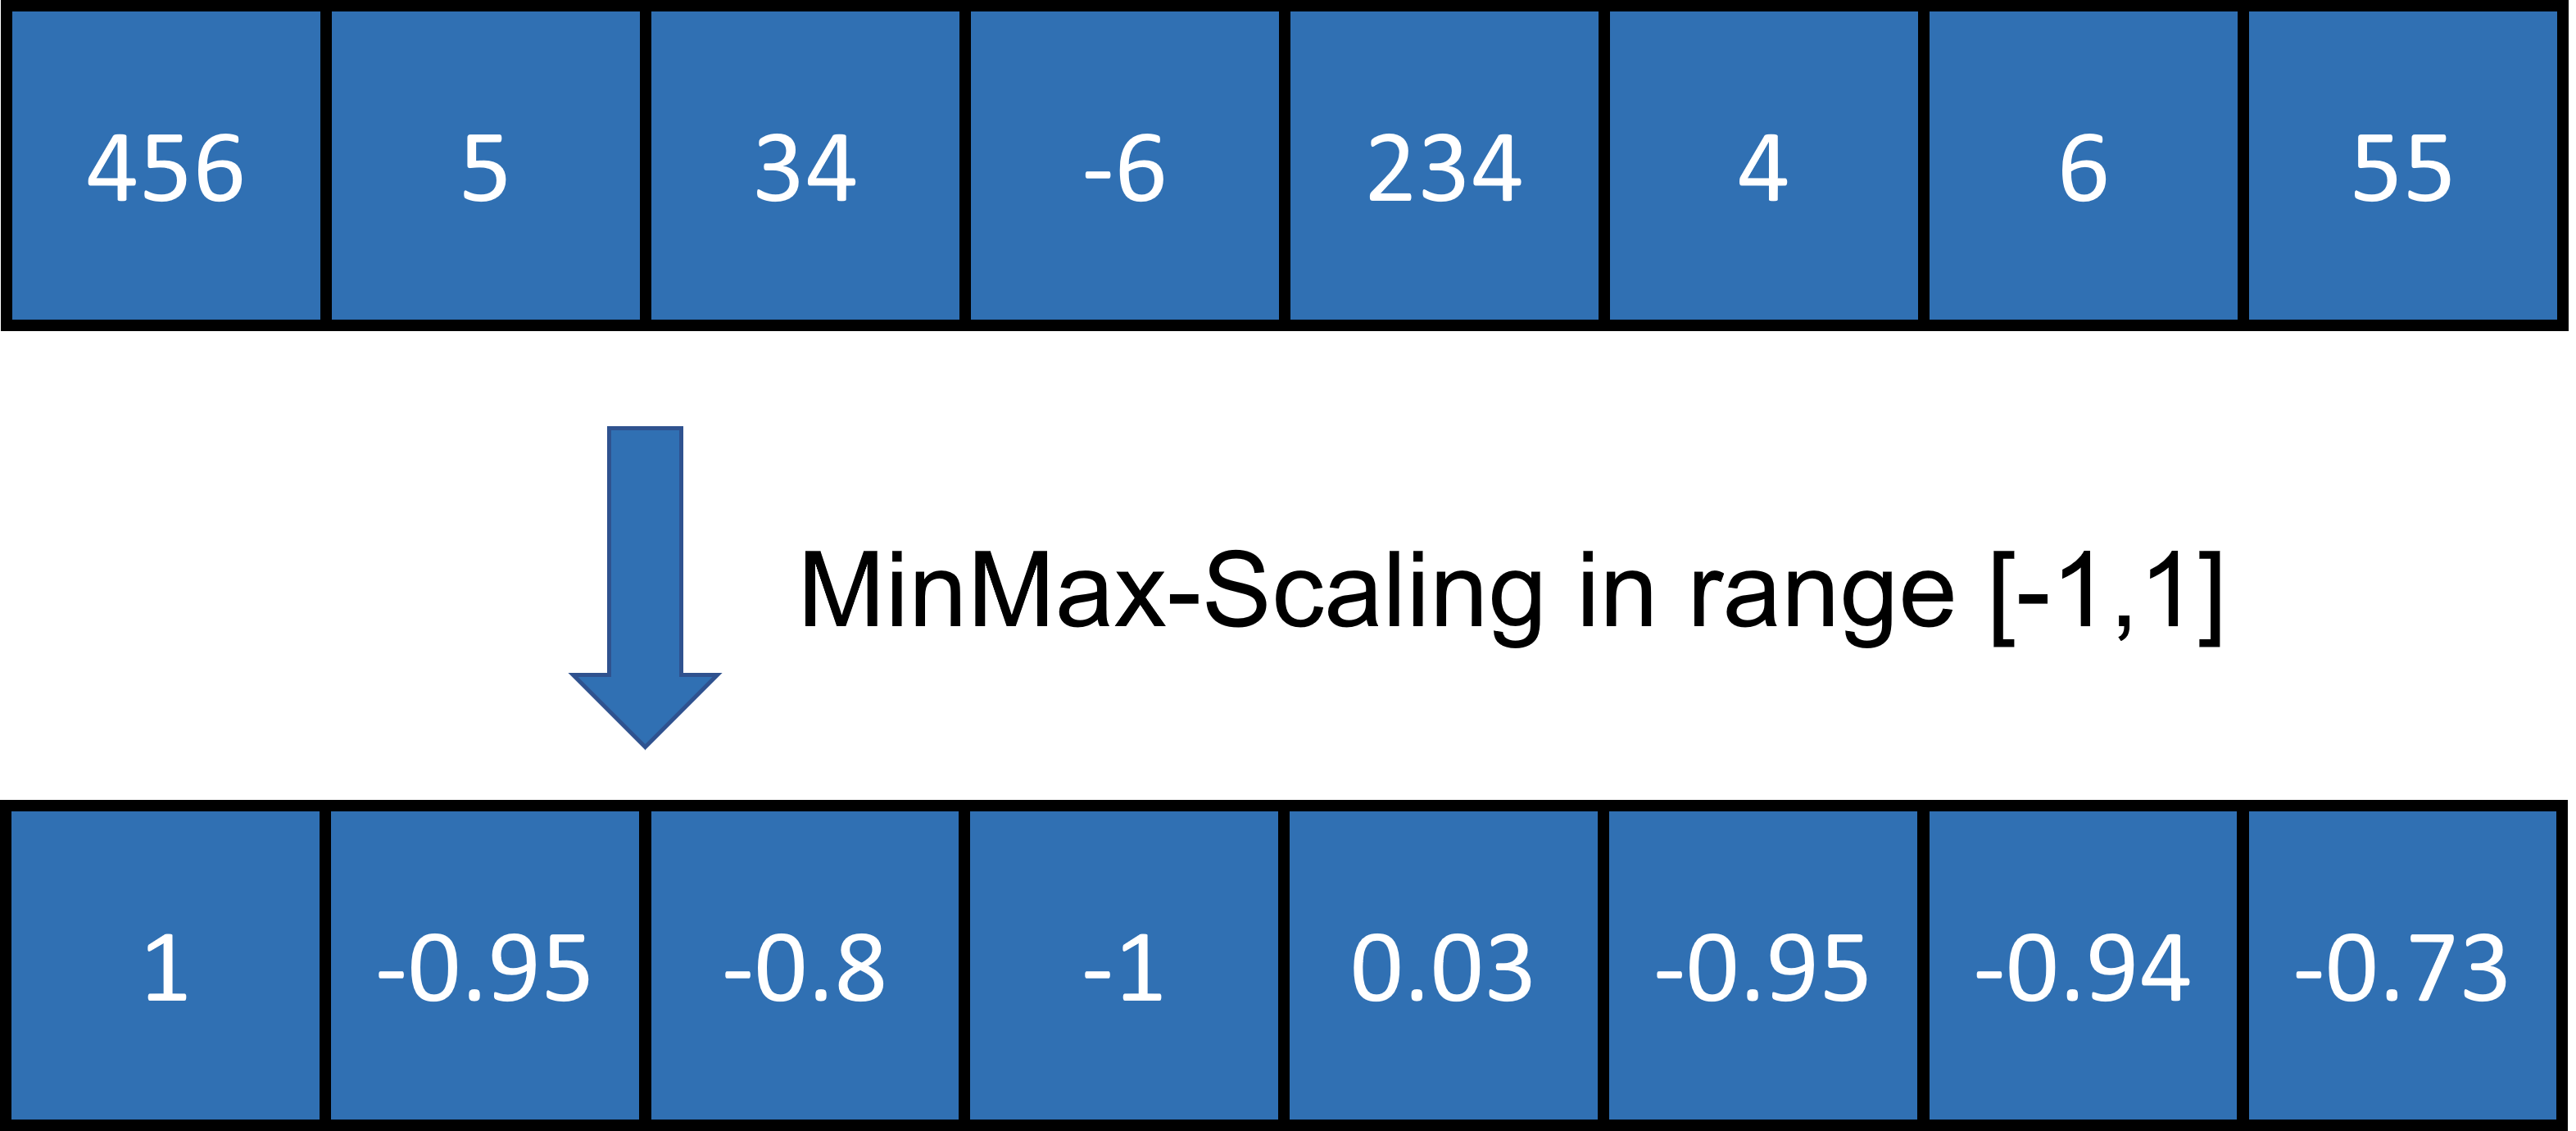
\includegraphics[width=0.5\linewidth]{IMGs/MM.png}
	\caption{Applying a MinMax-Scaler to a feature vector}
	\label{fig:MM}
\end{figure}


\subsubsection*{Hyperparameter}
Before a ML model can be trained, a set of hyperparameters needs to be defined that characterize the model and its behavior.
Most of the time, they are set manually, relying on the user's intuition or taken from literature \cite{Philipp}. 
For optimal performance, it requires extensive knowledge of the selected algorithm and how different combinations of parameters affect each other.
Exemplary hyperparameters are: learning rate, loss function, activation function or weights of neurons in NN (see chapter \ref{NN chapter}) \cite{Yang2}.
As hyperparameters play a very important role in the success of a ML model, specialized algorithms are in development for optimal hyperparameter selection \cite{Bergstra}.


\subsubsection*{K-fold Cross Validation}\label{KCV}
K-fold Cross Validation (KCV), is an approach for error estimation of ML models \cite{Zhang}. By applying KCV, the data-set is split into k subsets. All but one subset are used for training and the remaining one is used to measure the model's performance after it is trained. For that, the error-function is used. The score is saved, and the process is repeated for all k subsets \cite{Yoshua}. In the end, all k subsets were used once to assess the model. The expected value over all k-iterations is the final estimation of the models' performance. By employing this process, the model's sensitivity to one particular data-set does not influence the final rating of the model's performance \cite{Bishop}.



%https://web.archive.org/web/20170829124122id_/https://www.elen.ucl.ac.be/Proceedings/esann/esannpdf/es2012-62.pdf
%https://link.springer.com/article/10.1007/s11222-009-9153-8
%https://ieeexplore.ieee.org/abstract/document/8698831


\subsection{Core Functionalities in Machine Learning}
The core functionalities of ML are Supervised Learning, Unsupervised Learning and Reinforcement Learning (RL) \cite{Theodoridis,Janiesch}. In the following, these three functionalities are discussed in more detail.
Semisupervised Learning is a mix of Supervised and Unsupervised Learning~\cite{Zhu}. Due to its rarity and specialized approach, it is not covered by the scope of this thesis.

\subsubsection*{Supervised Learning}\label{SUPER}
Supervised Learning is split up into two parts: \textbf{Classification} and \textbf{Regression} \cite{Janiesch,Theodoridis}.

In the case of \textbf{Classification}, the data element that a model is trained on has a label (class label)~\cite{Carleo}. For example, images that contain either cats or dogs. The image is the data. The label is a corresponding value of either 1 or 0, which represents the presence of either animal in one specific image (for example, 0 for cats and 1 for dogs). The goal is to predict if a new image contains cats or dogs. The model that is used in the case of Classification is called a classifier~\cite{Theodoridis}.

To return the correct label, the classifier has to train on the available trainig-set, and find correlations between the data and labels~\cite{Carleo}.
After each training cycle, the prediction of the classifier can be compared to the true label (ground truth) and thus supervised on its performance.
\newpage
The classifier must learn the underlying structure (the pattern) of images and has to generalize, as the pictures in the test-set are not used in training and thus are unseen \cite{Bishop}. 
The found patterns allow the classification of the input (image) into discrete and limited variables (type of animal, 0 or 1) \cite{Theodoridis}.

Figure \ref{fig:CATDOG} shows a schematic representation of how a classifier is trained on a data-set containing images of either dogs or cats and how it is used to predict the label of a new image.

\begin{figure}[H]
	\centering
	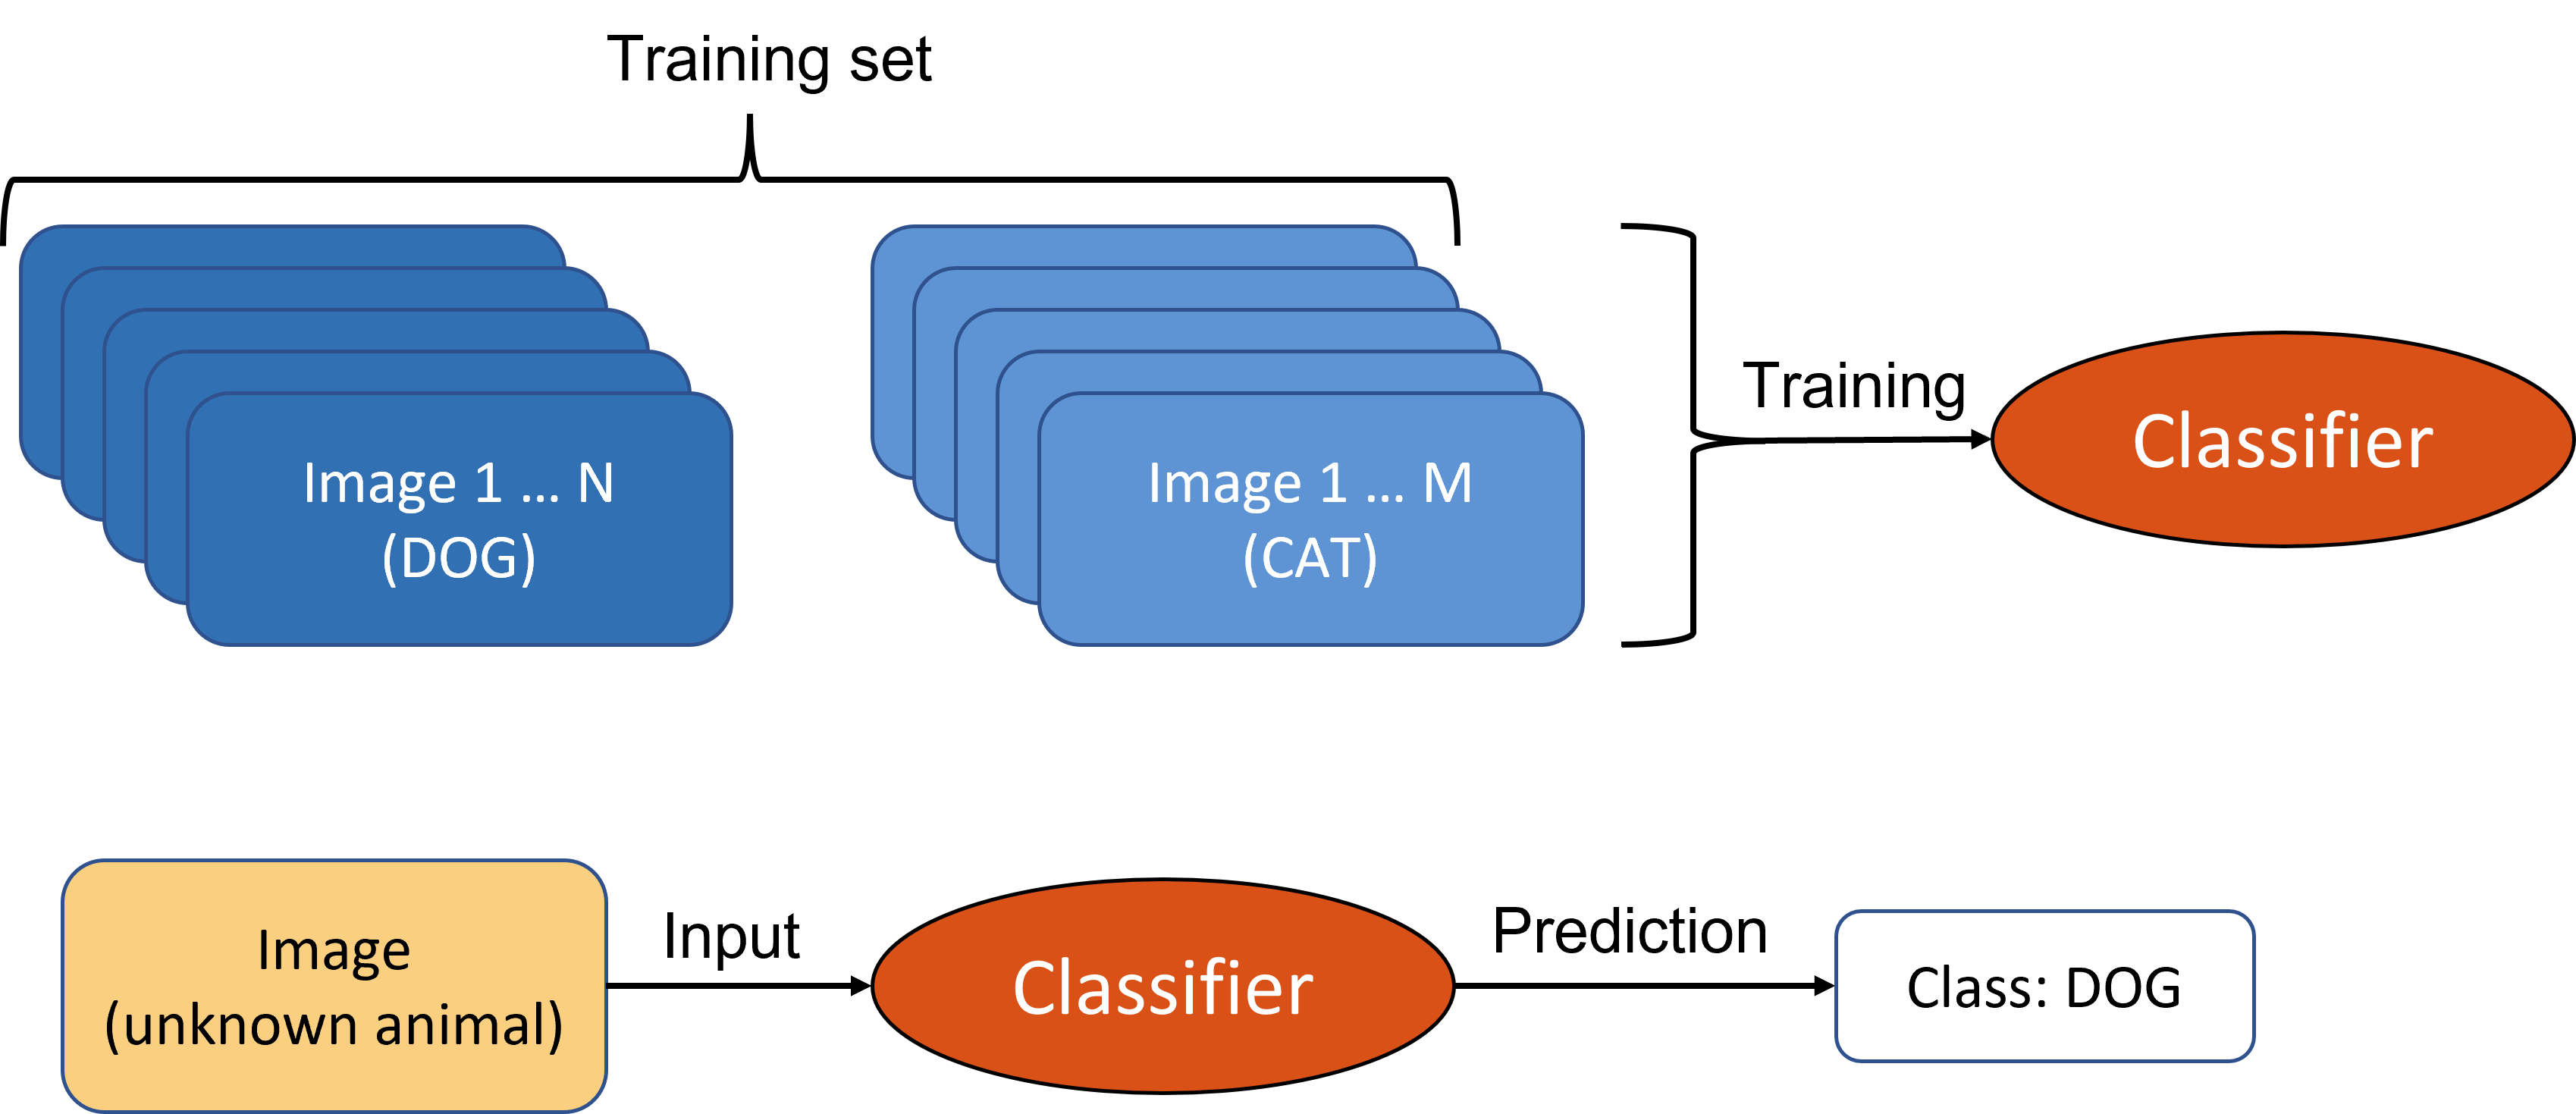
\includegraphics[width=0.9\linewidth]{IMGs/CATDOG.png}
	\caption{A schematic of the training and use of a classifier}
	\label{fig:CATDOG}
\end{figure}



Further examples of classifications are: the prediction of whether a tumor is benign or malignant or the authorship of a given text \cite{Theodoridis}.


The same basic principle is applied to \textbf{regression}. The main difference is that in the case of regression, the output is not a binary class but a continuous variable. In other words, the labels are lying in an interval. In broader terms, it is possible to call it a "curve fitting" method (see chapter \ref{TT}) \cite{Theodoridis}.

One application, for example, is to predict the position of the sun based on a picture containing shadows. The data in this case is, just as in the classification, the image. The label, on the other hand, is now a number that is the solar azimuth angle. The model can fit a function to the available data points and predict the sun's position on a new (unseen) picture.
An even more simple example is shown in figure \ref{fig:SimpleRegression}. A given data-set contains values of points in the \(x\)-\(y\) plane. With a regression model, the mapping function is estimated. Now the estimated function can be used to predict the \(y\)-value for a new \(x\)-value. 

\begin{figure}[H]
	\centering
	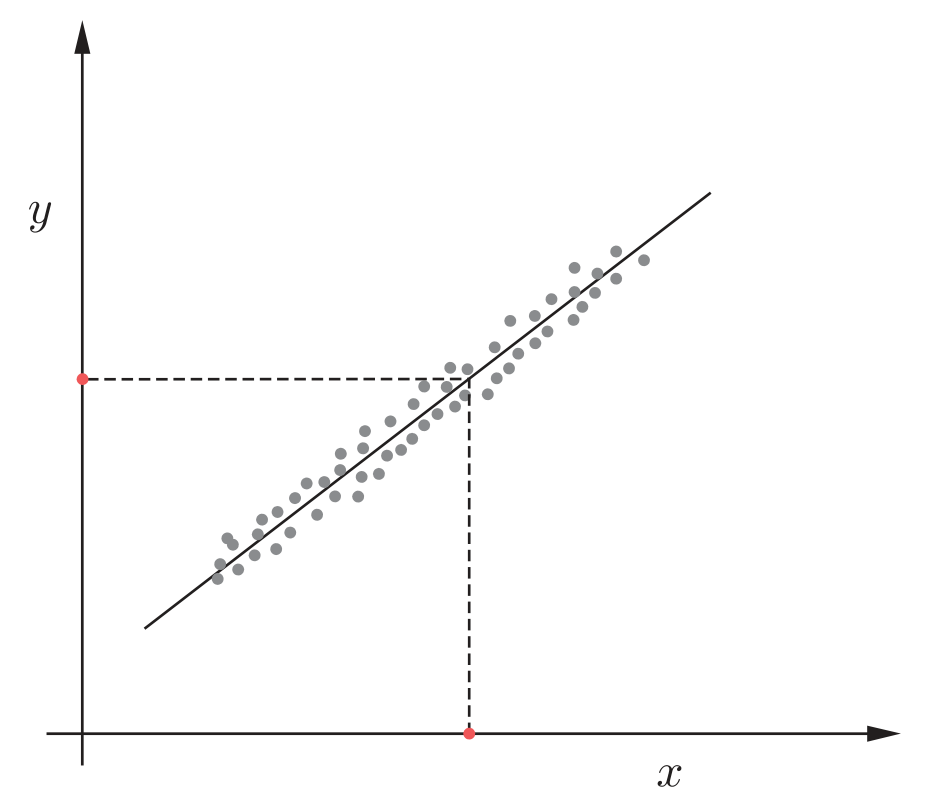
\includegraphics[width=0.5\linewidth]{IMGs/SimpleRegression.png}
	\caption{A mapping function based on a data-set containing \(x\) and \(y\) values \cite{Theodoridis}}
	\label{fig:SimpleRegression}
\end{figure}


Another example of regression is to predict a stock price in the next few minutes based on the history of the last 30 minutes \cite{Janiesch}.



\subsubsection*{Unsupervised Learning}
In Unsupervised Learning, the data that is given to a model has no labels. The goal of that method (just like in Supervised Learning) is to also find underlying patterns \cite{Carleo}. But instead of learning a pattern and comparing the output to the ground-truth, the method is designed in such a way that it discovers a pattern on its own \cite{Murphy}. The focus is not on assigning labels to an input, but on deciding to which class it belongs.

When applying this method to images, the output of the model are groups of pictures, where every group has something in common. Unsupervised Learning is very similar to human learning, as most things are learned without someone explicitly explaining how something works \cite{Murphy}. As mentioned in section \ref{Advantages and Problems of Machine Learning}, large labeled datasets are very difficult to create. Unsupervised Learning does not require a label and is thus widely applicable.

Figure \ref{fig:USL} visualizes how an unsupervised learning approach can divide a set of shapes based on their geometric properties. Class 1 contains shapes that are mostly round and class 2 contains shapes that are angular. 

\begin{figure}[H]
	\centering
	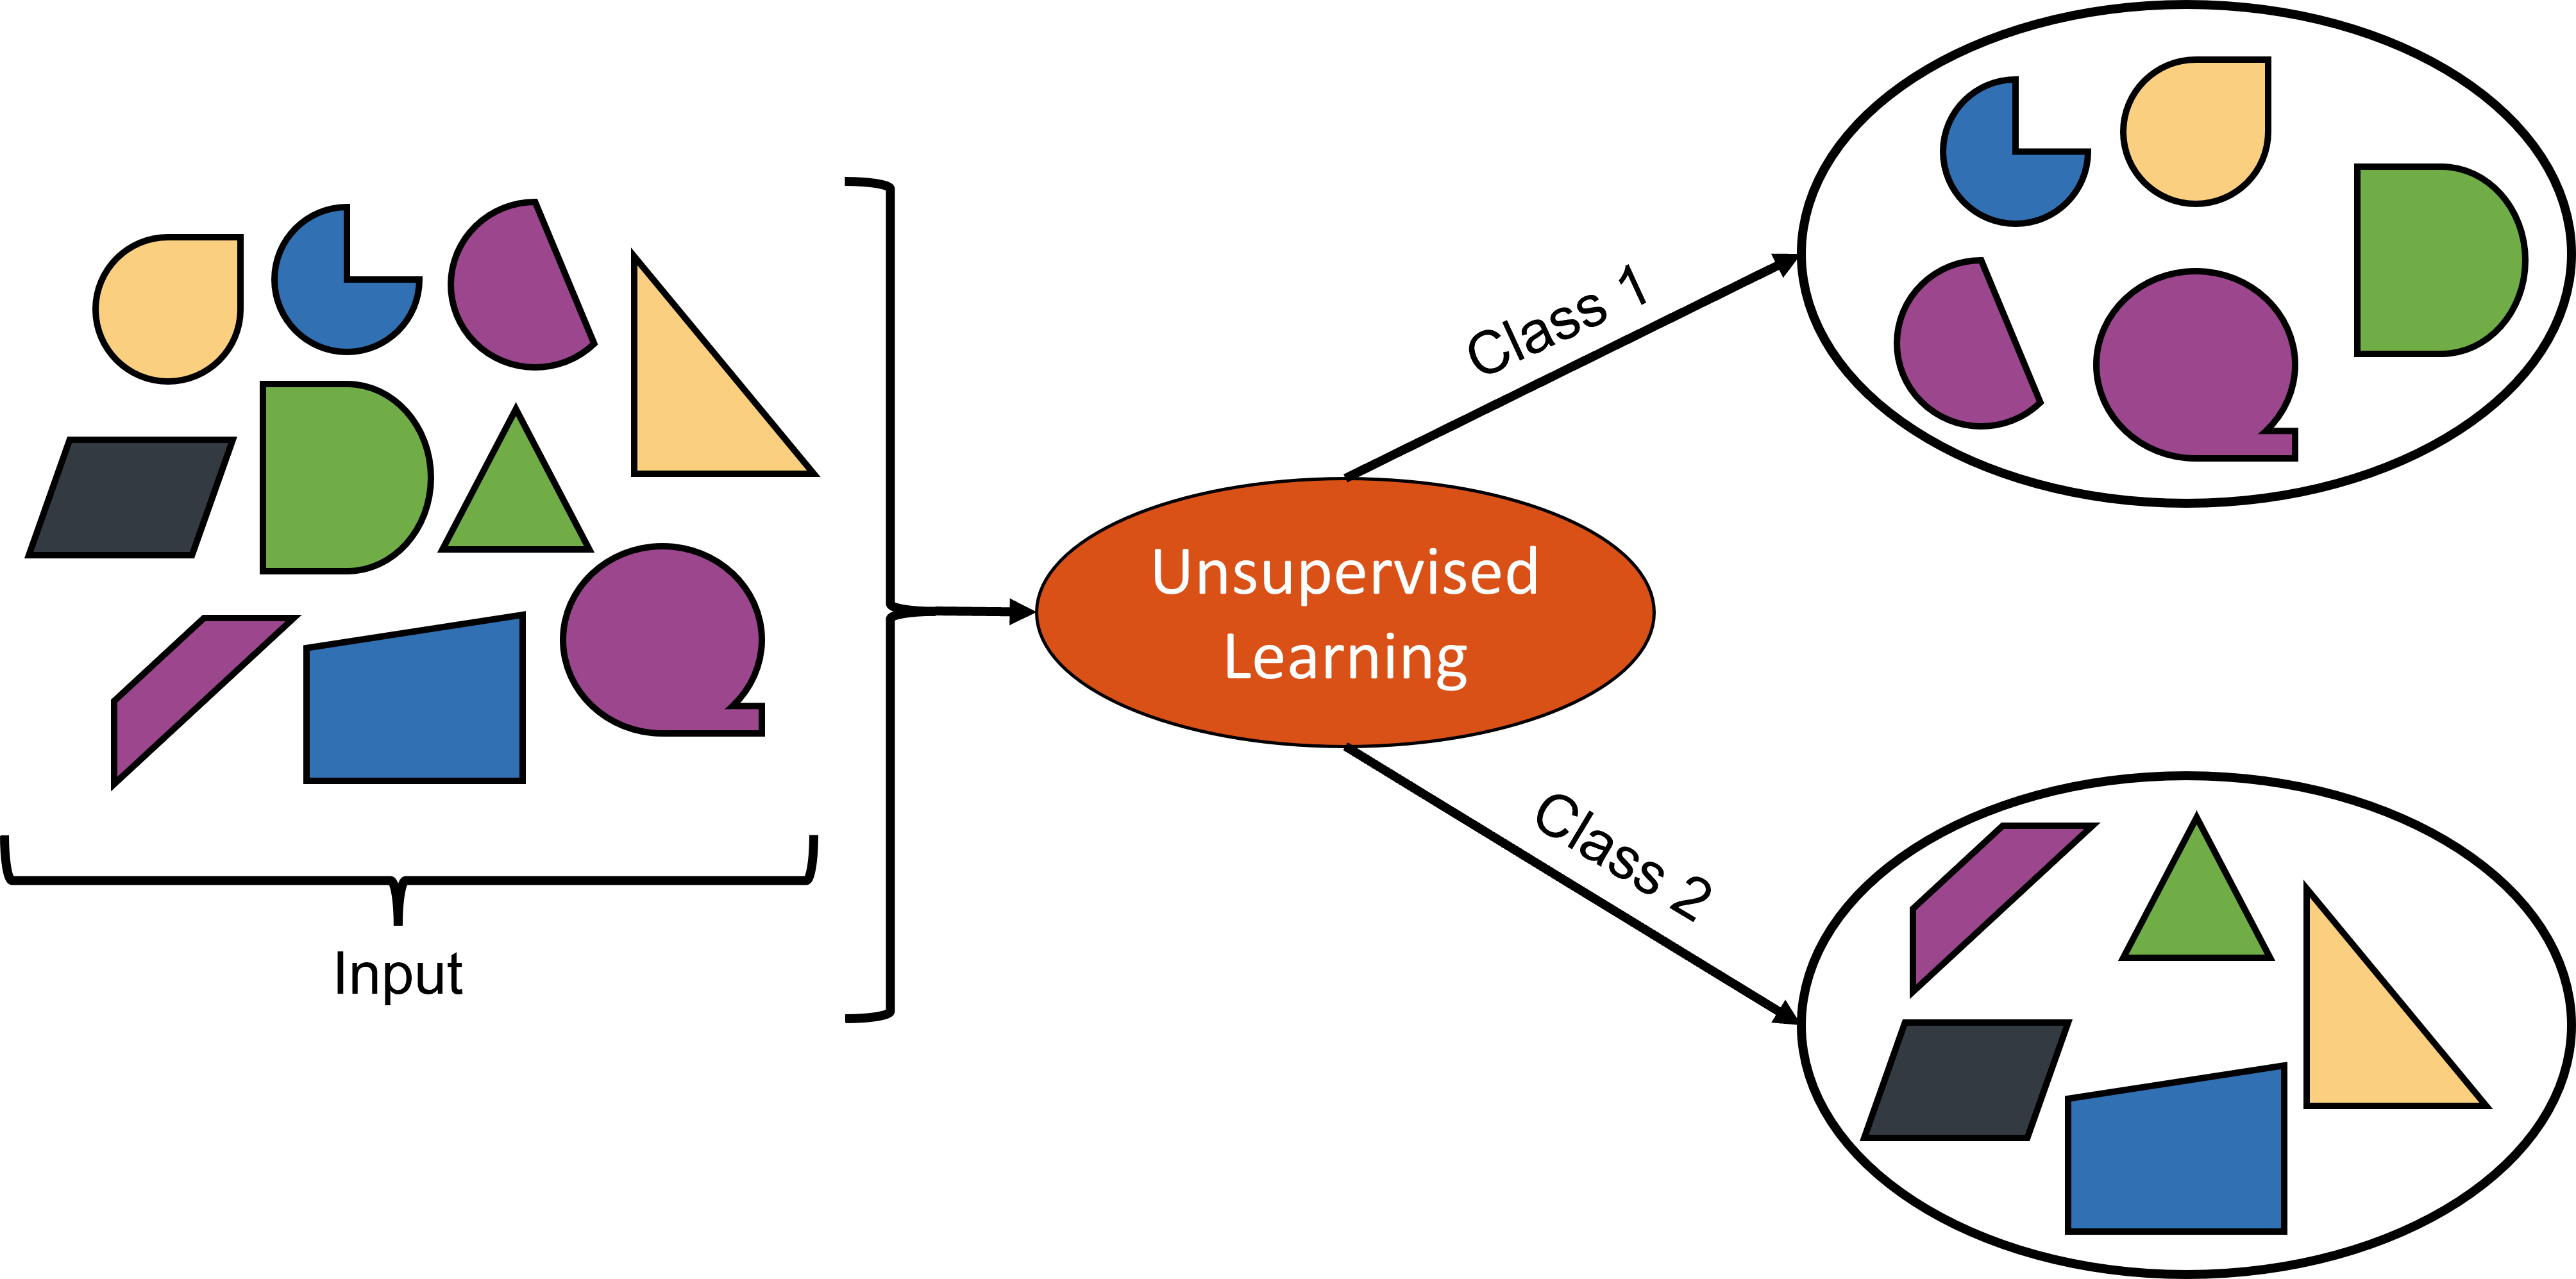
\includegraphics[width=0.9\linewidth]{IMGs/USL.png}
 	\caption{Finding similarities in shapes and grouping them into classes}
 	\label{fig:USL}
\end{figure}


\subsubsection*{Reinforcement Learning}

RL is based on the same principle as the learning process in people or animals. The main objective is to reach a goal or, in other words, to maximize a numerical value. The learning process is in a loop with observing and decision-making. The so-called agent is in an environment that he can observe and perform action in. The actions are rewarded or punished with a numerical reward. \cite{LEX}
 
Actions that bring the agent closer to the goal are rewarded proportionally to their usefulness in achieving the goal. After completion of the task (achieving the goal) a large reward is issued to signal the agent that the steps taken were successful. As the agent does not know which actions lead to high rewards, it has a significant exploration part in the beginning of its training to confirm or update its assumptions regarding the predicted reward for each action in each state.~\cite{Sutton}

One of the most challenging tasks in RL is deciding which steps in the process were the good and bad ones. This is also called the "Credit Assignment Problem" \cite{Minsky,Bishop}. To solve a task, for example, finding a way out of a labyrinth, the agent has to first navigate in the opposite direction to the exit, to then again get closer to the exit. The three distinguishing parts of RL are: a closed loop system, no clear instructions, and the long-term strategy of the agent. \cite{Sutton}

Figure \ref{fig:SimpleRL} shows one iteration of the interaction of the agent with the environment. First, the agent receives the state of the environment as a feature vector. Based on that current state and the agent's long-term strategy, it performs an action and thus changes the environment. After performing the action, the agent is rewarded for its performance based on the defined goal~\cite{LEX}.

\begin{figure}[H]
	\centering
	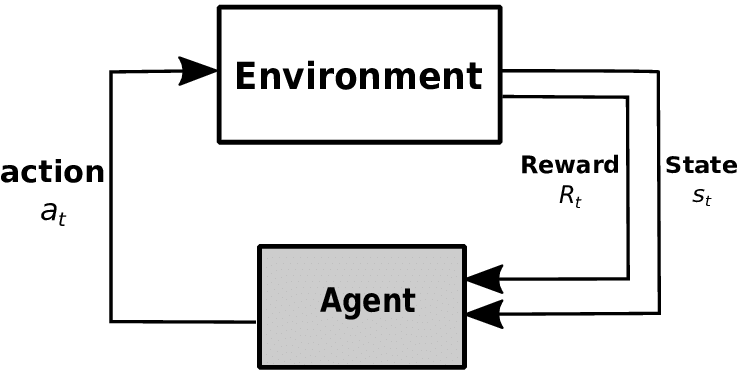
\includegraphics[width=0.5\linewidth]{IMGs/SimpleRL.png}
	\caption{The interaction of an agent with its environment in RL \cite{LEX}.}
	\label{fig:SimpleRL}
\end{figure}
RL finds a lot of applications in games and game-like scenarios, as the goal and reward are easily defined and the state of the environment is easily encoded into a feature vector \cite{Takuma}.
Due to the limited scope of this thesis and the nature of the problem described in chapter \ref{prob}, RL is not further discussed. More information can be found in \cite{Sutton}.
 

\subsection{Specialized Machine Learning Approaches}
In the following, three specialized architectures are presented and analyzed in more detail.
\subsubsection*{Neural Networks}\label{NN chapter}
NNs are based on the same principle as the functionality of the human brain \cite{Janiesch}.
The basic components of a NN in a living organism are neurons and synapses. The synapses are connecting the neurons with each other. Based on the input, a synapse can be activated or inhibited. Based on that observation, McCulloch and Pitts implemented a simple model, called a perceptron, that mimics exactly this behavior \cite{Theodoridis}.
Figure \ref{fig:2nn} shows how two neurons are connected to each other. This principle is reproduced many times to create a large NN out of perceptrons.
\begin{figure}[H]
	\centering
	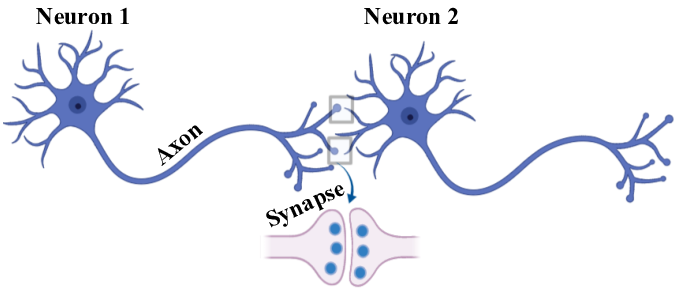
\includegraphics[width=0.8\linewidth]{IMGs/2NN.png}
	\caption{Connection of two neurons via synapses \cite{Das}}
	\label{fig:2nn}
\end{figure}
\newpage
NN are also referred to as Artificial Neural Networks (ANNs). These models are based on the same principle as the perceptron. In this case, the perceptrons are arranged in layers and referred to as nodes or neurons. The first layer is called an input layer and the last one is the output layer. The layers in between are called hidden layers \cite{JOOST}. 

Figure \ref{fig:NN1} shows an exemplary NN with three hidden layers. Each element of the input vector is given to one node at the input layer. This type of NN is also called a Feed-Forward Neural Network. Because the neurons are fully connected, it is also referred to as a fully connected NN \cite{Sainath}. Note that the output does not need to be a single value. It can also be a vector. In that case, the output layer would consist of multiple nodes.

\begin{figure}[H]
	\centering
	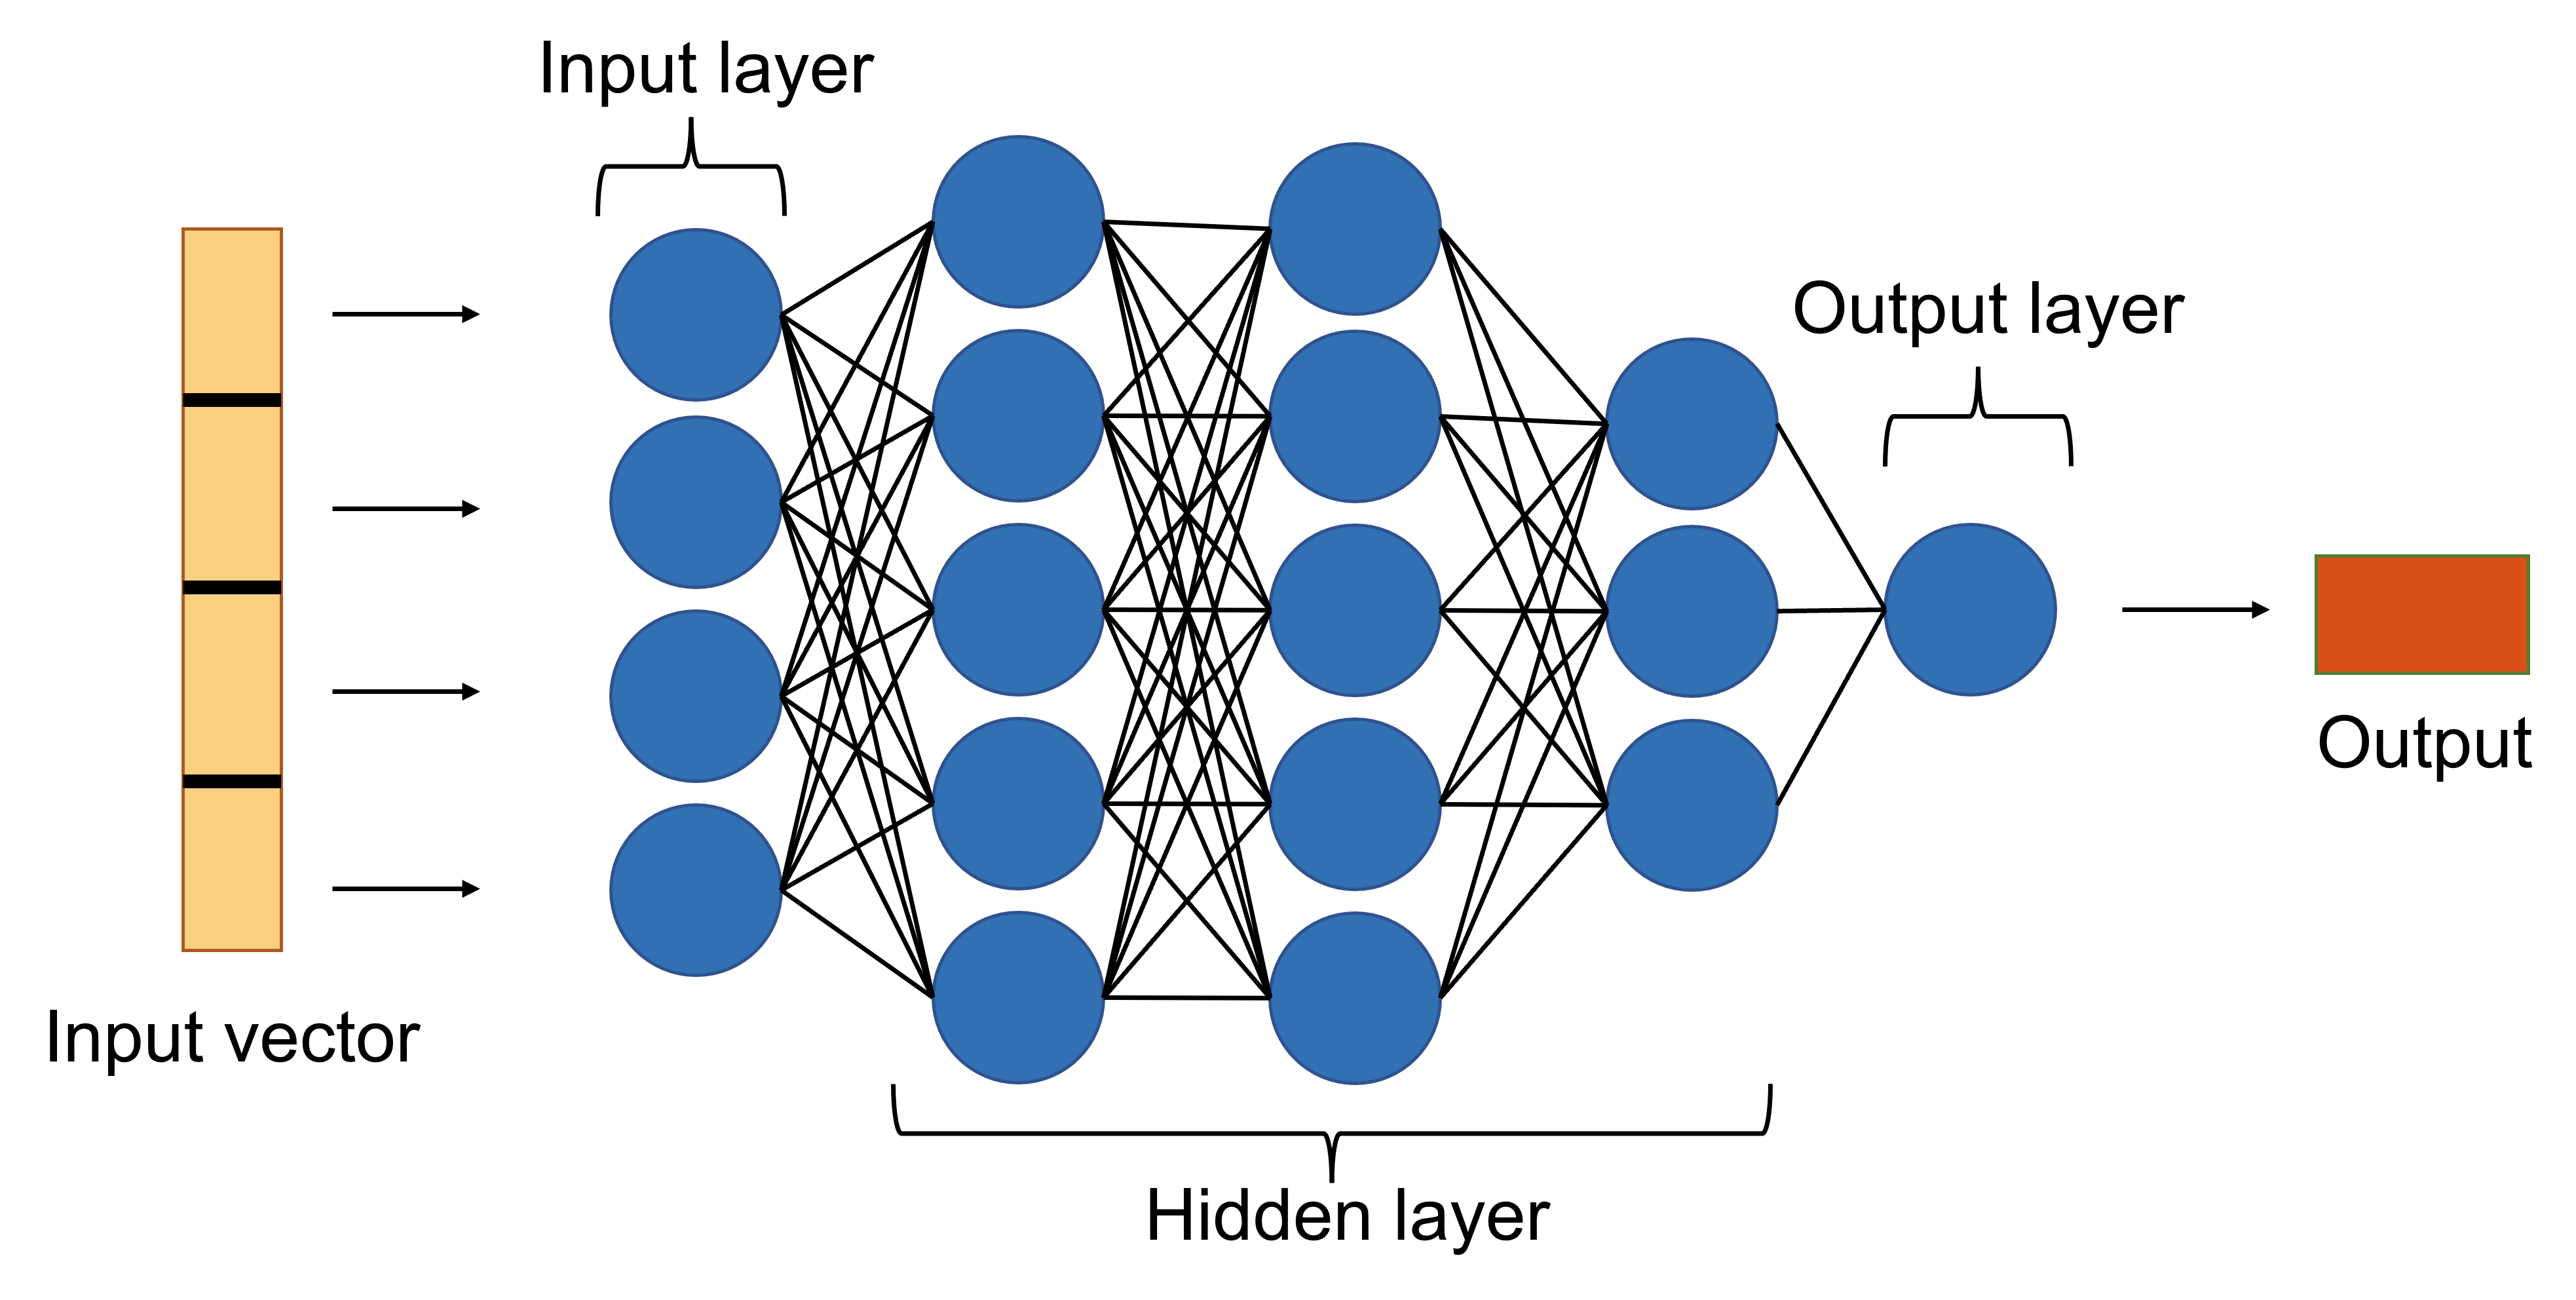
\includegraphics[width=0.8\linewidth]{IMGs/NN1.png}
	\caption{NN with three hidden layers}
	\label{fig:NN1}
\end{figure}
 
To model an organic NN more closely and improve the performance, the nodes have an activation function built into them, which can introduce non-linearity \cite{Goyal}. One of the most common activation functions is the "rectified linear unit" (ReLU) \cite{Goodfellow}. Figure \ref{fig:AF} shows three common activation functions. The most common activation functions are: ReLU, sigmoid, tanh and softmax \cite{Activation}

\begin{figure}[H]
	\centering
	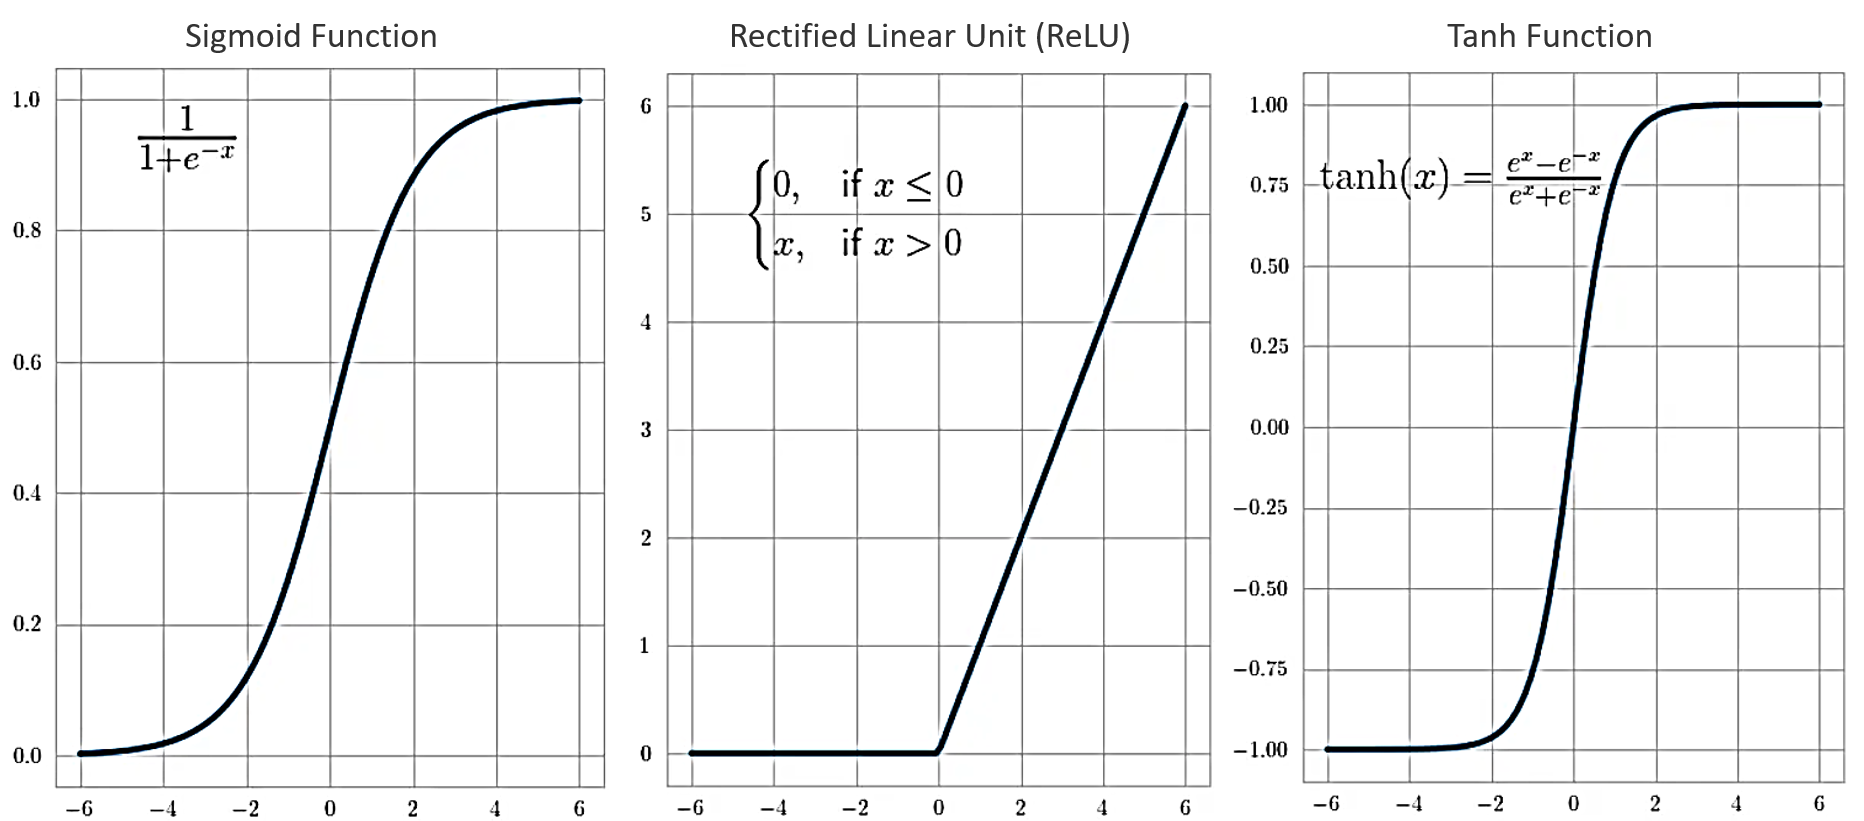
\includegraphics[width=0.8\linewidth]{IMGs/Active.png}
	\caption{Various activation functions for NNs \cite{Activation}}
	\label{fig:AF}
\end{figure}

Figure \ref{fig:PC} shows the basic functionality of a neuron at the first hidden layer. The ouput-elements of the input layer are pre-multiplied with individual values called weights and summed up to a single value. This value is processed by the activation function and returns the output for that specific neuron for that specific input \cite{BattaMahesh}. The output value is then used as input in the following hidden layers \cite{Ding}. The adjustments of those weights is done in training through a process called back-propagation \cite{Chauvin}. 
It is important to note that the activation functions can be chosen for each layer individually. Especially in classification, the activation function at the output layer is most commonly set as SoftMax while in the previous layers as ReLU \cite{Asadi}. 

\begin{figure}[H]
	\centering
	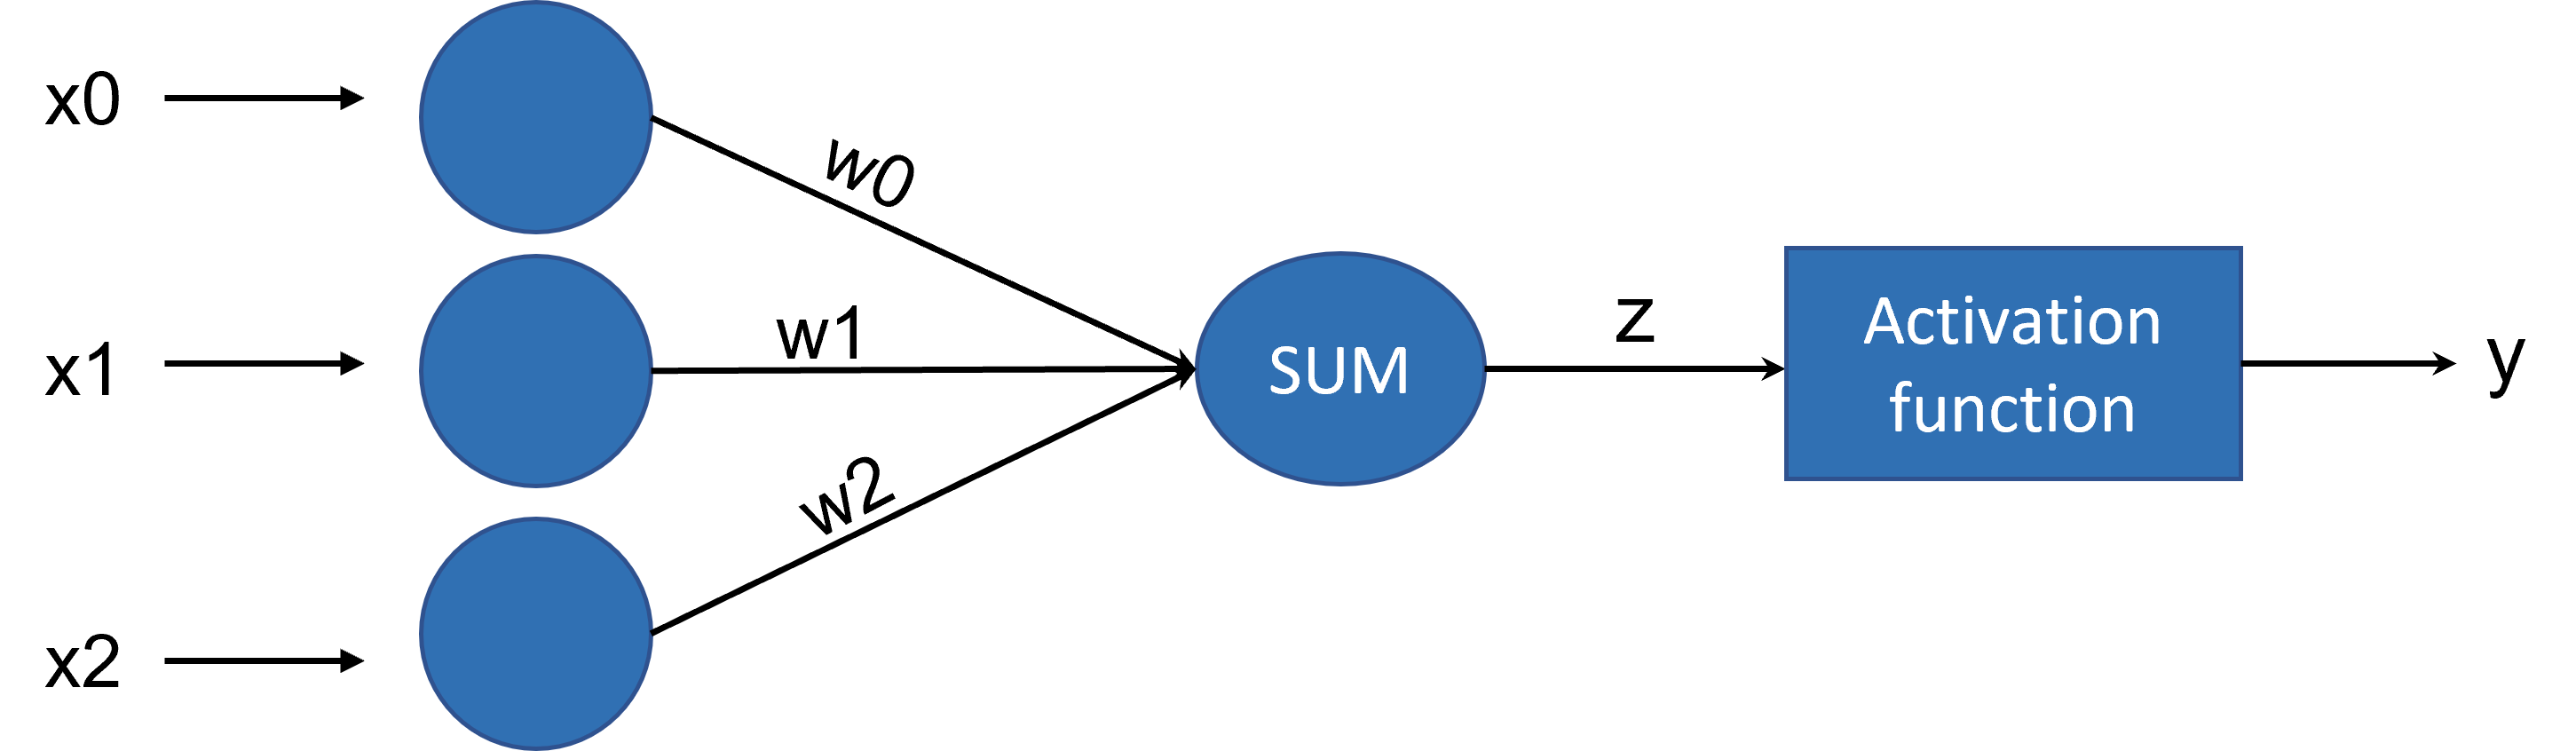
\includegraphics[width=0.8\linewidth]{IMGs/PEC.png}
	\caption{Graphical representation of a perceptron \cite{Ding}}
	\label{fig:PC}
\end{figure}

Deep Neural Networks (DNNs) are NNs that contain many hidden layers. The increased amount of parameters and non-linearity helps them achieve better feature abstraction and learn more complex patterns \cite{JOOST}.
The biggest disadvantage of DNNs and DL in general is that even more data is necessary to optimally tune the free parameters \cite{Thompson}. Further, DL is very computationally expensive and requires significantly more time for training \cite{Fu}. 





\subsubsection*{Recurrent Neural Networks}
Recurrent Neural Networks (RNNs) are specialized NNs that are designed to be applied to problems involving time-series data, like sensor data or ordered data like sentences \cite{Jain}. After each input, the neurons in a RNN are sending feedback signals to the following and some previous nodes. By doing that, a cycle is formed \cite{Grossberg}. By having this feedback loop to previous nodes, the output is dependent on the new input and the output from the previous input. This specialized architecture can pay attention to the sequence of the input data \cite{Jain}.

The rest of the functionality is almost the same as in a conventional NN. Figure \ref{fig:rnn} shows a simple RNN. The output of the first layer is sent back to the nodes C1 and C2. In this case, they are called context units. With this structure, the RNN can "remember" the input from the previous input. These closed-loop cycles are the "memory" of the RNN \cite{Salehinejad}.

\begin{figure}[H]
	\centering
	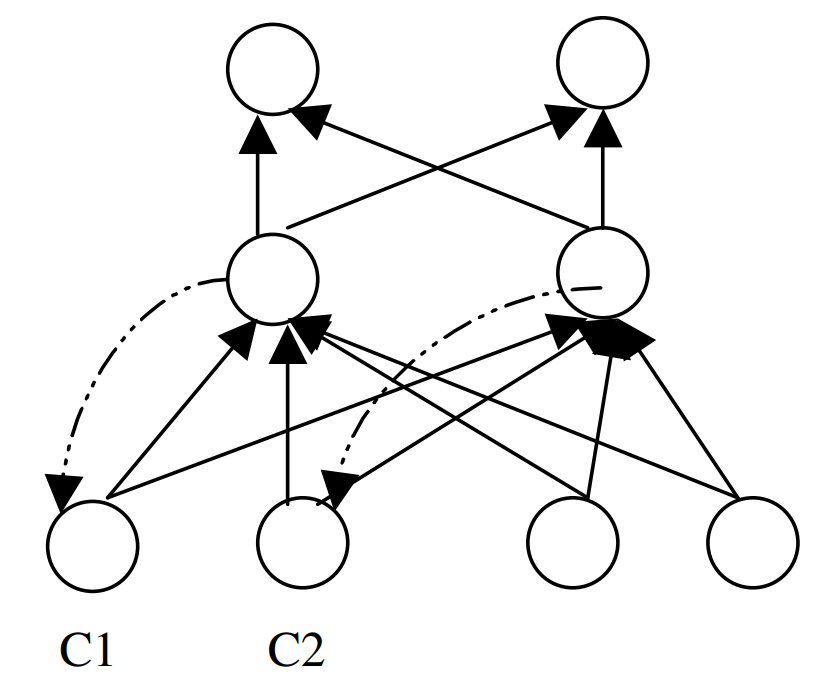
\includegraphics[width=0.4\linewidth]{IMGs/rnn.png}
	\caption{Simple RNN \cite{Jain}}
	\label{fig:rnn}
\end{figure}

By using the memory-structure, RNNs are capable of understanding sequential dependencies. A conventional RNN is capable of remembering up to ten time-steps (inputs) back. By adding more recurrent connections with the goal of increasing the memory-capacity, the gradient of the response is either exponentially increasing to infinity or decreasing to 0 \cite{Staudemeyer}. Thus, a standard RNN is limited in its ability to remember a lot of data.

Figure \ref{fig:rnn2} shows how a RNN can be unfolded. The recurrent structure is unfolded in the time-domain and gives a clear understanding of how the output of a cell at time \(t_0\) is used as additional input at time \(t_1\).

\begin{figure}[H]
	\centering
	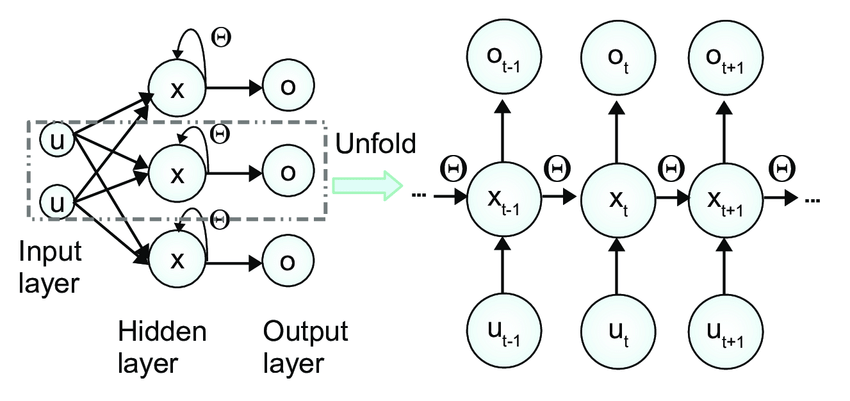
\includegraphics[width=0.8\linewidth]{IMGs/RNN2.png}
	\caption{Unfolded structure of a RNN \cite{Guo}.}
	\label{fig:rnn2}
\end{figure}


A subgroup of RNNs are long-short- term memory RNNs (LSTMs). LSTMs are able to learn correlation of even longer sequences than conventional RNNs \cite{Salehinejad}. LSTMs are capable of remembering more than 1,000 time-steps \cite{Staudemeyer}.

LSTM-networks are finding more and more areas of application. For example, in machine health monitoring or load prediction in power stations \cite{Zhao,Muzaffar}. The similarity between those applications is the dependency of the output on recent and past inputs. 

\subsubsection*{Physics Informed Neural Networks}
Physics-informed Neural Networks (PINNs) are special types of NNs that are capable of following defined boundary conditions like laws of physics \cite{Cai}. One of the most used application domain, are problems involving partial differential equations (PDEs). Instead of using the available data to discover the physics from scratch, prior knowledge can be incorporated through the PDEs \cite{Cuomo}. By utilizing PINNs, a simple NN architecture can be used, that requires less training time, and can achieve equivalent results to large NNs \cite{Misyris}.

Figure \ref{fig:piml} shows the basic functionality of a PINN. The overall goal is to minimize the error function, just as in function fitting (see chapter \ref{TT}). In this case, the error function is made up of the initial- and boundary-conditions as well as the constraints of the PDE \cite{Guo}. The training process is analogue to the standard NN approach. 
\begin{figure}[H]
	\centering
	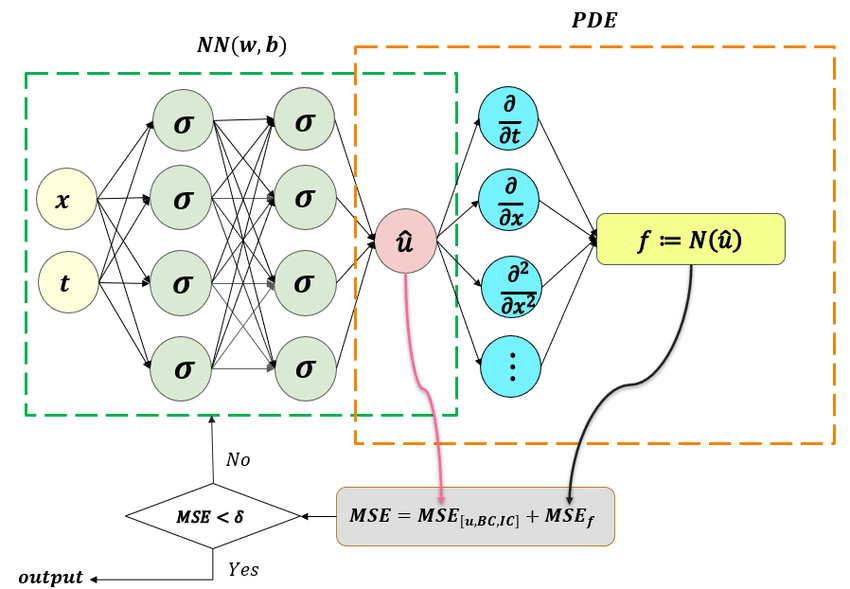
\includegraphics[width=0.7\linewidth]{IMGs/piml.png}
	\caption{Schematic diagram of a PINN \cite{Guo}.}
	\label{fig:piml}
\end{figure}




\newpage
\section{Overview of Machine Learning in Industry Applications}
In the following, the application of ML in engineering and industrial applications is discussed.
\subsection{General Application of Machine Learning in Industry}
The possibilities of ML are extending to many areas of application \cite{Deiana}. The analysis of recent publications in \cite{Bertolini}, concluded four main categories of ML for industrial applications. Table \ref{MLIND} gives to each category an example.

\begin{table}
	\begin{center}
		\begin{tabular}{|| l | l ||}
			\hline
			\rule{0pt}{2ex}Application Domain: & Example:\\
			\hline
			\hline
			\rule{0pt}{2ex}Maintenance Management & Failure modes classification and prediction\\\hline
			Quality Management & Defects detection and classification\\	\hline
			Production Planning and Control & Job scheduling and dispatching\\\hline
			Supply Chain Management & Demand planning and forecasting\\
			\hline
		\end{tabular}
		\caption{Main categories of ML for industrial applications \cite{Bertolini}.}
		\label{MLIND}
	\end{center}
	\vspace{-4mm}
\end{table}
When comparing the implemented ML-approaches, Supervised Learning clearly dominates each category. When looking at the total field, each ML-approach (Supervised, Unsupervised and RL) experienced a significant growth increase over the last 20 years \cite{Bertolini}. This is an indicating factor that ML will play an important role in the future for engineering sciences.

Condition Monitoring and Predictive Maintenance (which are both in the domain "Maintenance Management") are closely related to the explained problem in chapter \ref{prob}.
Condition monitoring is the continuous analysis of parameters that correlate to the machines operation and maintenance \cite{Rao}. Predictive Maintenance is a preventive maintenance program. Instead of scheduling maintenance activities after a failure has occurred, predictive maintenance uses condition monitoring to run the machines as long as possible (close to failure) to eliminate unnecessary downtime through premature stopping or unexpected delays through unforeseen failures \cite{Mobley}.

It is important to note that Predictive Maintenance and Condition Monitoring are also performed with other tools, like statistical analysis and do not solely rely on ML \cite{Carvalho, Divya}. 


 
\subsection{Comparison of Machine Learning in Gear Applications}
The process of calculating heath indicators has gained a lot of interest in engineering in the past years. By correctly assessing a systems' state, accidents and unexpected downtime can be avoided \cite{Wang}. In this section, the application of ML in Condition Monitoring and Predictive Maintenance of gears is analyzed.

The basis of heath indicators are signals or values coming from the physical system itself. Vibration, noise, electrical current and thermal images can be used for fault detection or to determine the state-of-damage in gears \cite{Prav,KaraACUSTIC,Medina,Kara}

By using the vibration signal, it is possible to determine gear damage like tooth cracks and face wear. These kinds of damage can introduce vibrations, that travel to other parts of the system like the gearbox housing. By having an accelerometer on the housing, the vibrations can be detected and analyzed. The proposed method in \cite{Prav} was able to successfully make a distinction between a faulty and a healthy gear. This method however, did not make any prediction regarding the progressing state of health of the gears and only analyzed them in their current state-of-damage. 

The approach in \cite{Medina} uses a LSTM network to determine the progressing level of pitting. The input signal is classified into nine levels of severity of damage. The pitting damage was created artificially by Electrical Discharging Machining (EDM). The input data is an acoustic recording of 15 seconds. In total 1215 samples are recorded. After prepossessing and encoding, the LSTM could successfully classify each signal into the correct class of pitting damage.

The method applied in \cite{RTiwari} also uses vibration signals to perform a classification. In this approach, a Support Vector Machine (SMV) is used to classify healthy and worn gears. The goal is to classified different gears based on their damage. Some gears had chipped or missing teeth. This approach also achieved a high success rate. No attention is given in regards of the change of variation over a long period of time to determine a state-of-damage. 


These approaches are not transferable to the problem described in chapter \ref{prob}. When the datasets for those methods are constructed, the gears were already in the state that is used as a label (healthy, damaged).

When trying to transfer this approach to get a better prediction than the Miner rule, the input would be the load-history and the label the true state-of-damage or range of it. But calculating the physically accurate damage sum D is not possible. Thus, these approaches are not capable of solving the problem at hand. 

Over the last decade, significant advancements are also continuously made in the area of predicting the Remaining-Useful-Life (RUL) of machine elements \cite{Deutsch,He,Yan}.
The biggest problem with those models and approaches, is the assumed constant load that is acting on the components. Due to this assumption, these approaches can not be transferred to machinery where the cyclic loads have a significant variance in amplitude over time.

In summery, no methods were published that use a-priori knowledge of the Miner rule and the known load sequence to determine a more confident state-of-damage in machine elements.


% !TeX spellcheck = en_US 
\chapter{Methodology}\label{MET}
This chapter discusses the methodology that uses load sequences that ended in fatigue failure, to get a confidence value for the accumulated damage sum D of a load sequence that did not yet end in failure. Each step of the proposed method is discussed in detail. Chapters \ref{DA} and \ref{DV} give an introduction to the data, while chapter \ref{GO} serves as general guidance. Detailed explanations begin in chapter \ref{SBOC}.

\section{Data Acquisition}\label{DA}
The load sequences are acquired by performing a Single Tooth Bending Fatigue Test (STBF). A gear is held in place by two teeth clamped in a test rig. A hydraulic piston is applying cyclical loading until bending fatigue failure occurs. The loading profile is manually defined for each test. The loading profile consists of a force level and the number of cycles during which this force is applied. Instead of constructing the loading sequence from the predetermined parameters (force and repetitions), a force sensor is used that records the net force of a cycle that occurs at its peak. This is done to simulate real machinery, where the loading history is also measured and not created by a-priori available hyperparameters. 
Figure \ref{fig:STBFT} shows an exemplary test rig for STBF tests.
\begin{figure}[H]
	\centering
	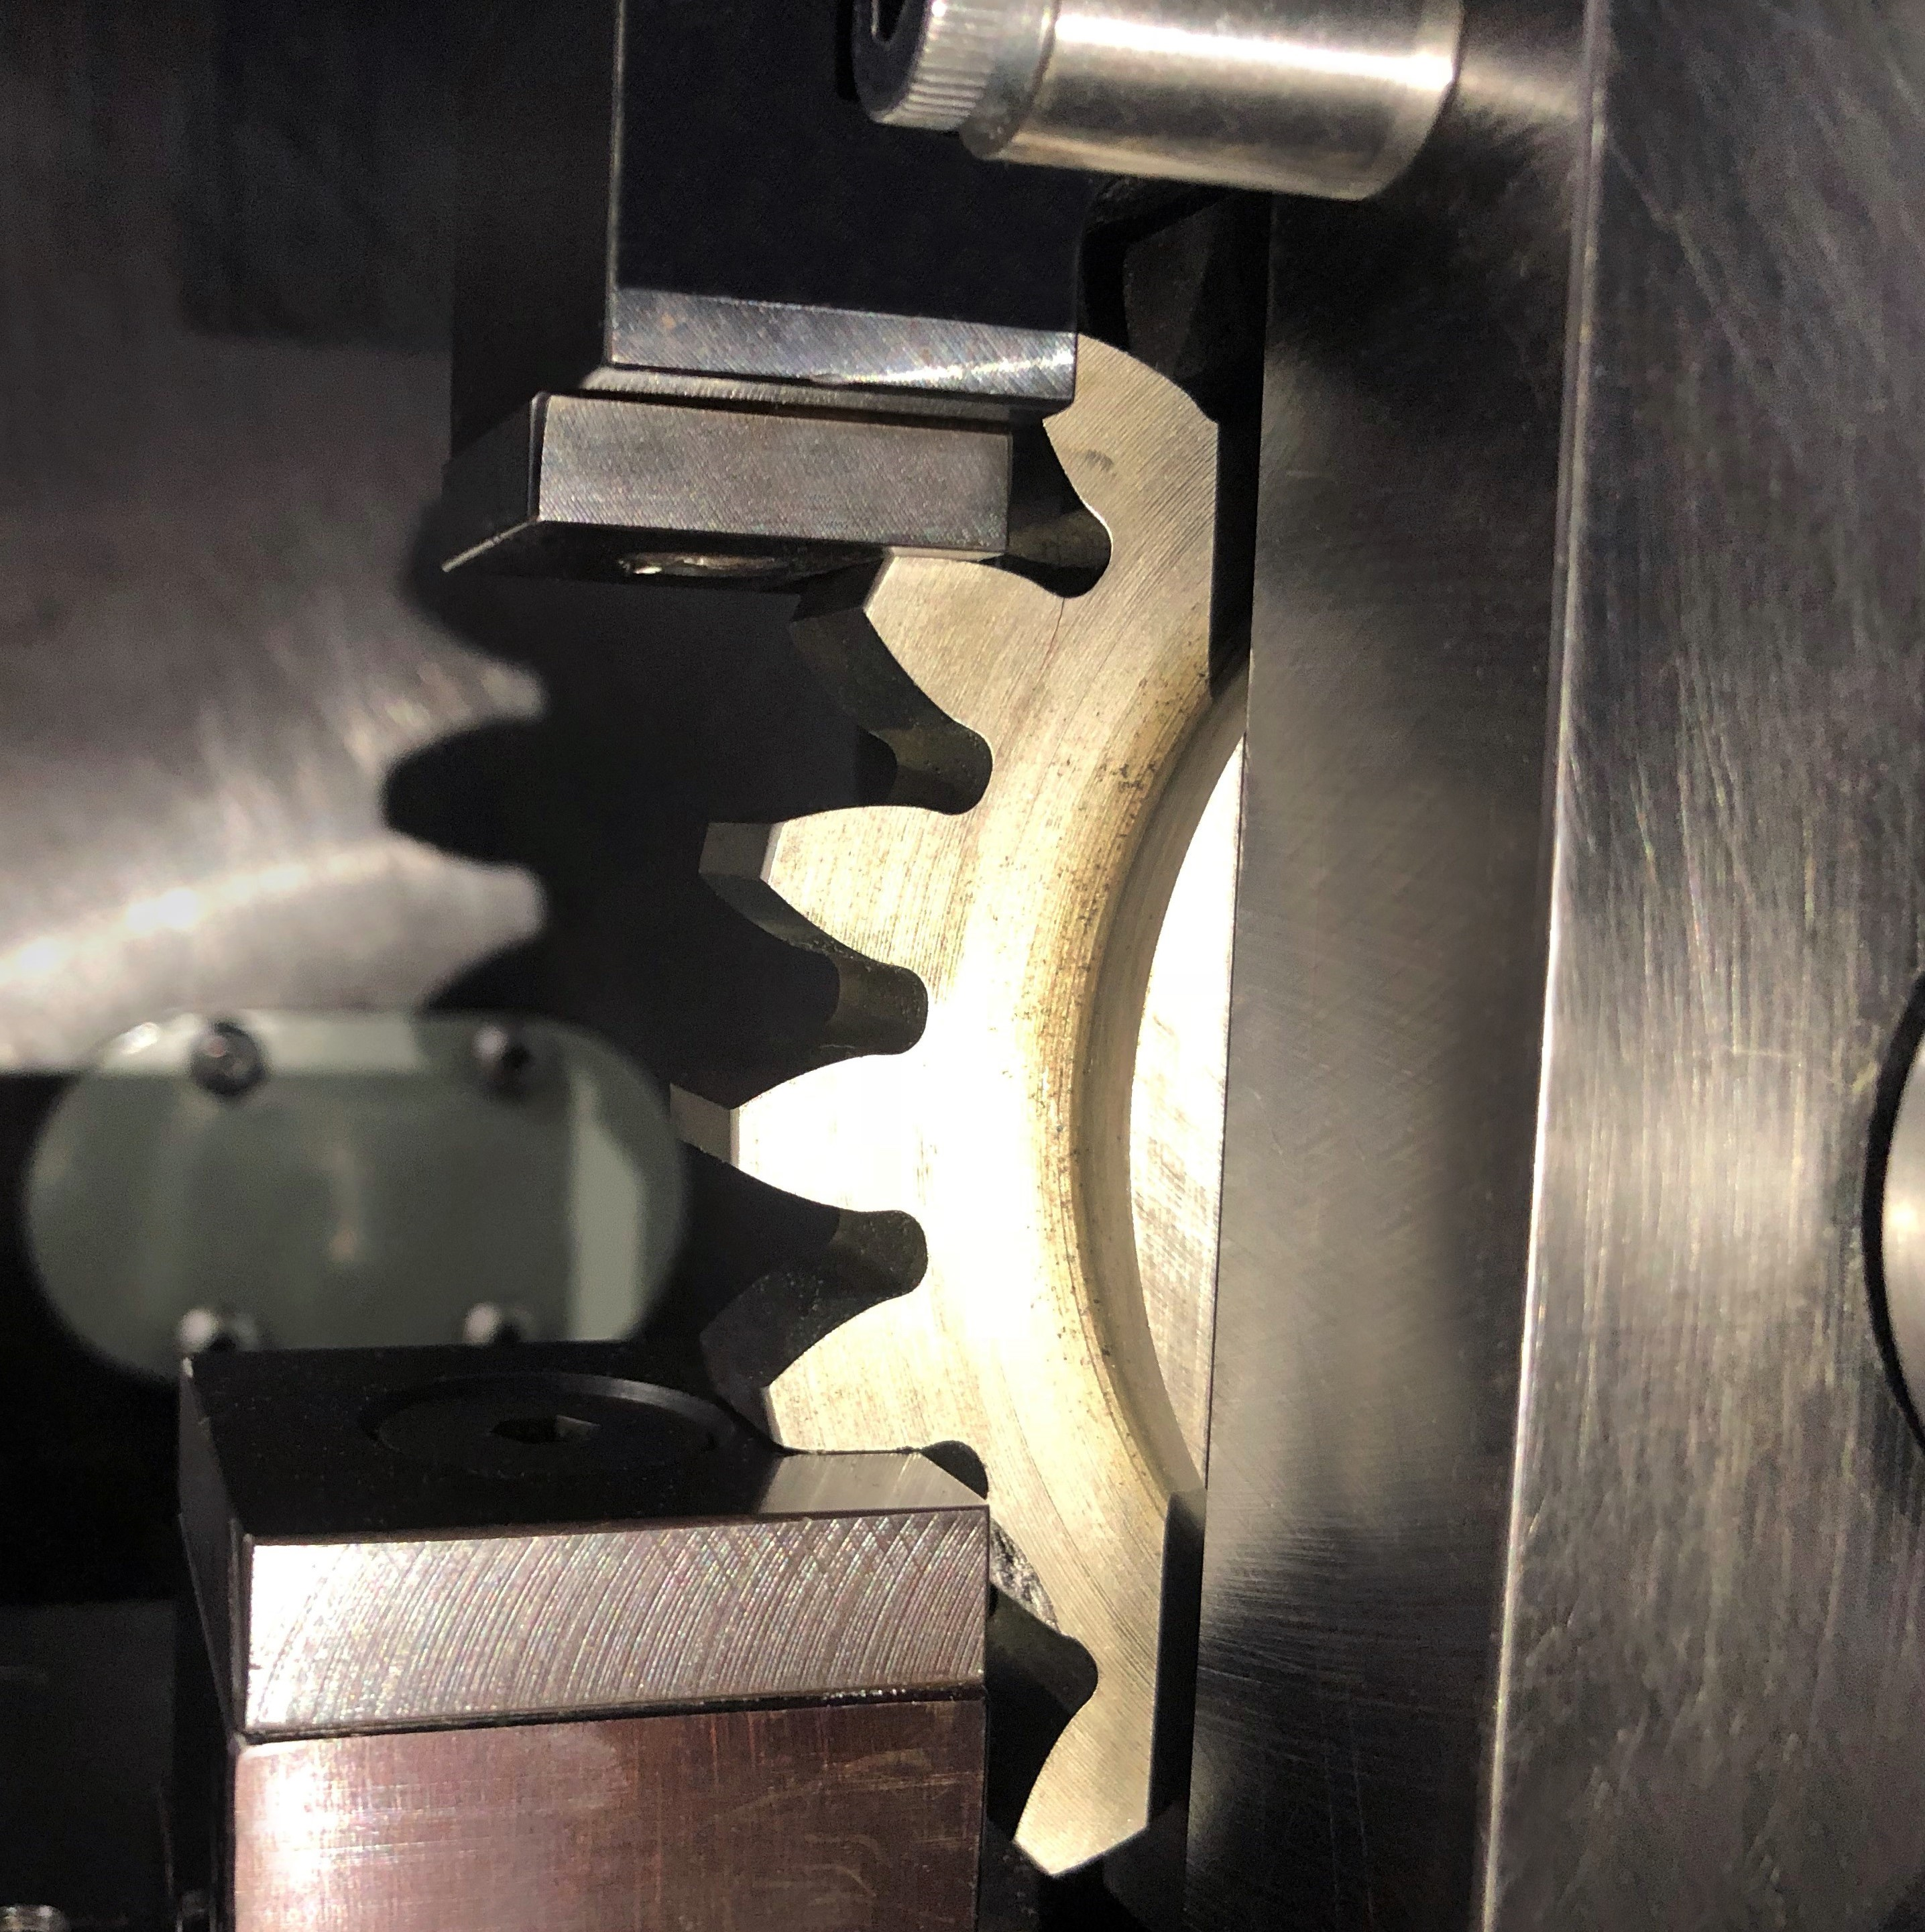
\includegraphics[width=0.5\linewidth]{IMGs/tooth.jpg}
	\caption{Test rig for Single Tooth Bending Fatigue Test (STBF) \cite{STBT}}
	\label{fig:STBFT}
\end{figure}
\newpage

\section{Data Visualization}\label{DV}
Figures \ref{fig:L1}, \ref{fig:L2} and \ref{fig:L3}  show three different load sequences. The \(x\)-axis denotes the number of the cycle in that sequence, and the \(y\)-axis the applied force. As the force is acting in the negative direction with regards to the defined coordinate system, it is recorded with a negative sign. The clamping force is set to 3kN. The sudden reduction of force in the load history appears when the test rig switches from one load-level to another. 
Additionally, the vertical lines represent the damage sum D according to Miner at 0.5, 0.8 and 1. Note that failure is expected at a damage sum equal to 1. The tested gear with the load sequence presented in figure \ref{fig:L2} was able to accumulate a damage sum D greater than unity and thus exceeding its expected failure point. The applied load sequence shown \ref{fig:L3} resulted in early failure.

\begin{figure}[H]
	\centering
	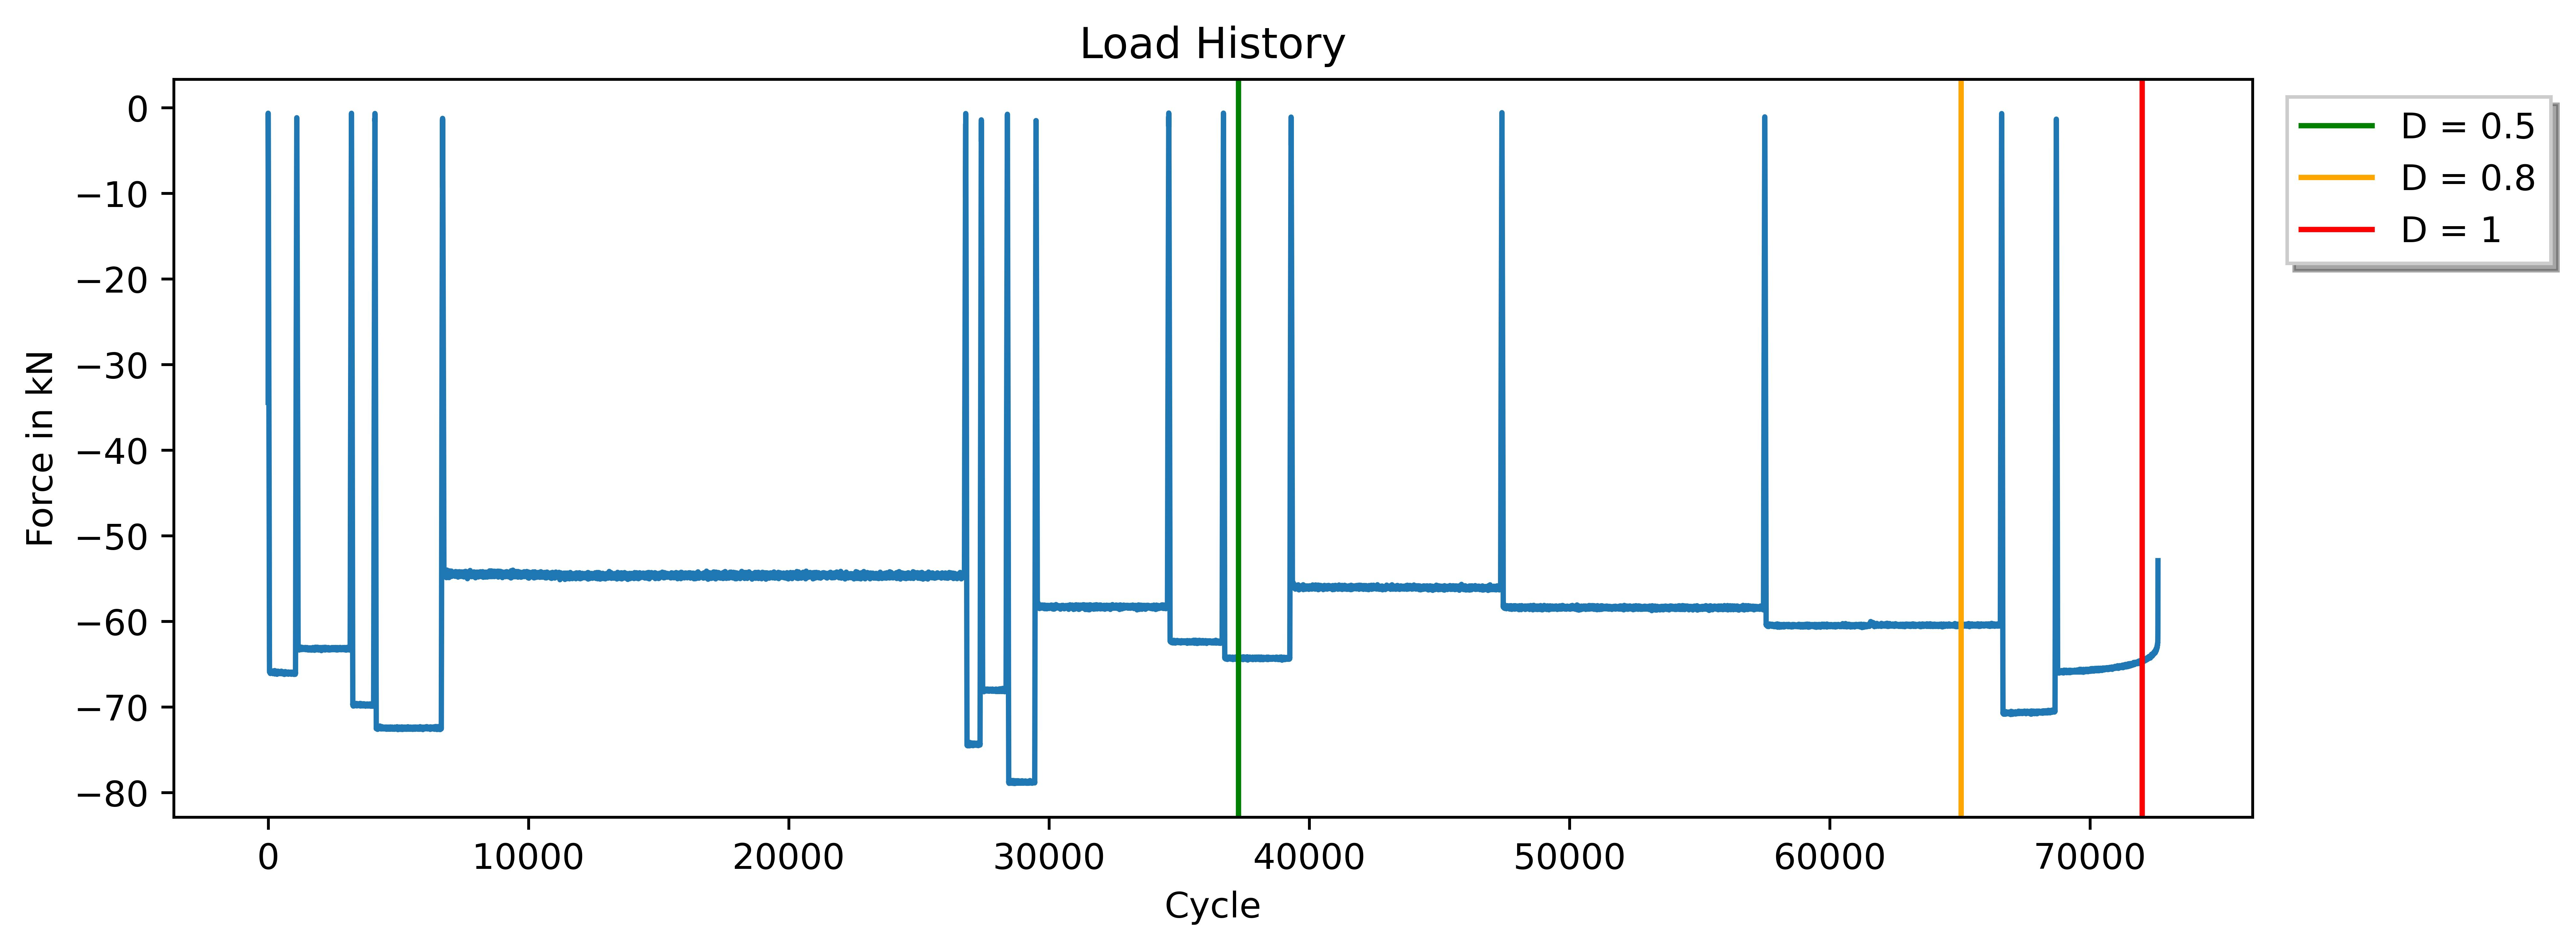
\includegraphics[width=1\linewidth]{IMGs/Load/L0.jpg}
	\caption{Load sequence with failure close to D=1}
	\label{fig:L1}
\end{figure}

\begin{figure}[H]
	\centering
	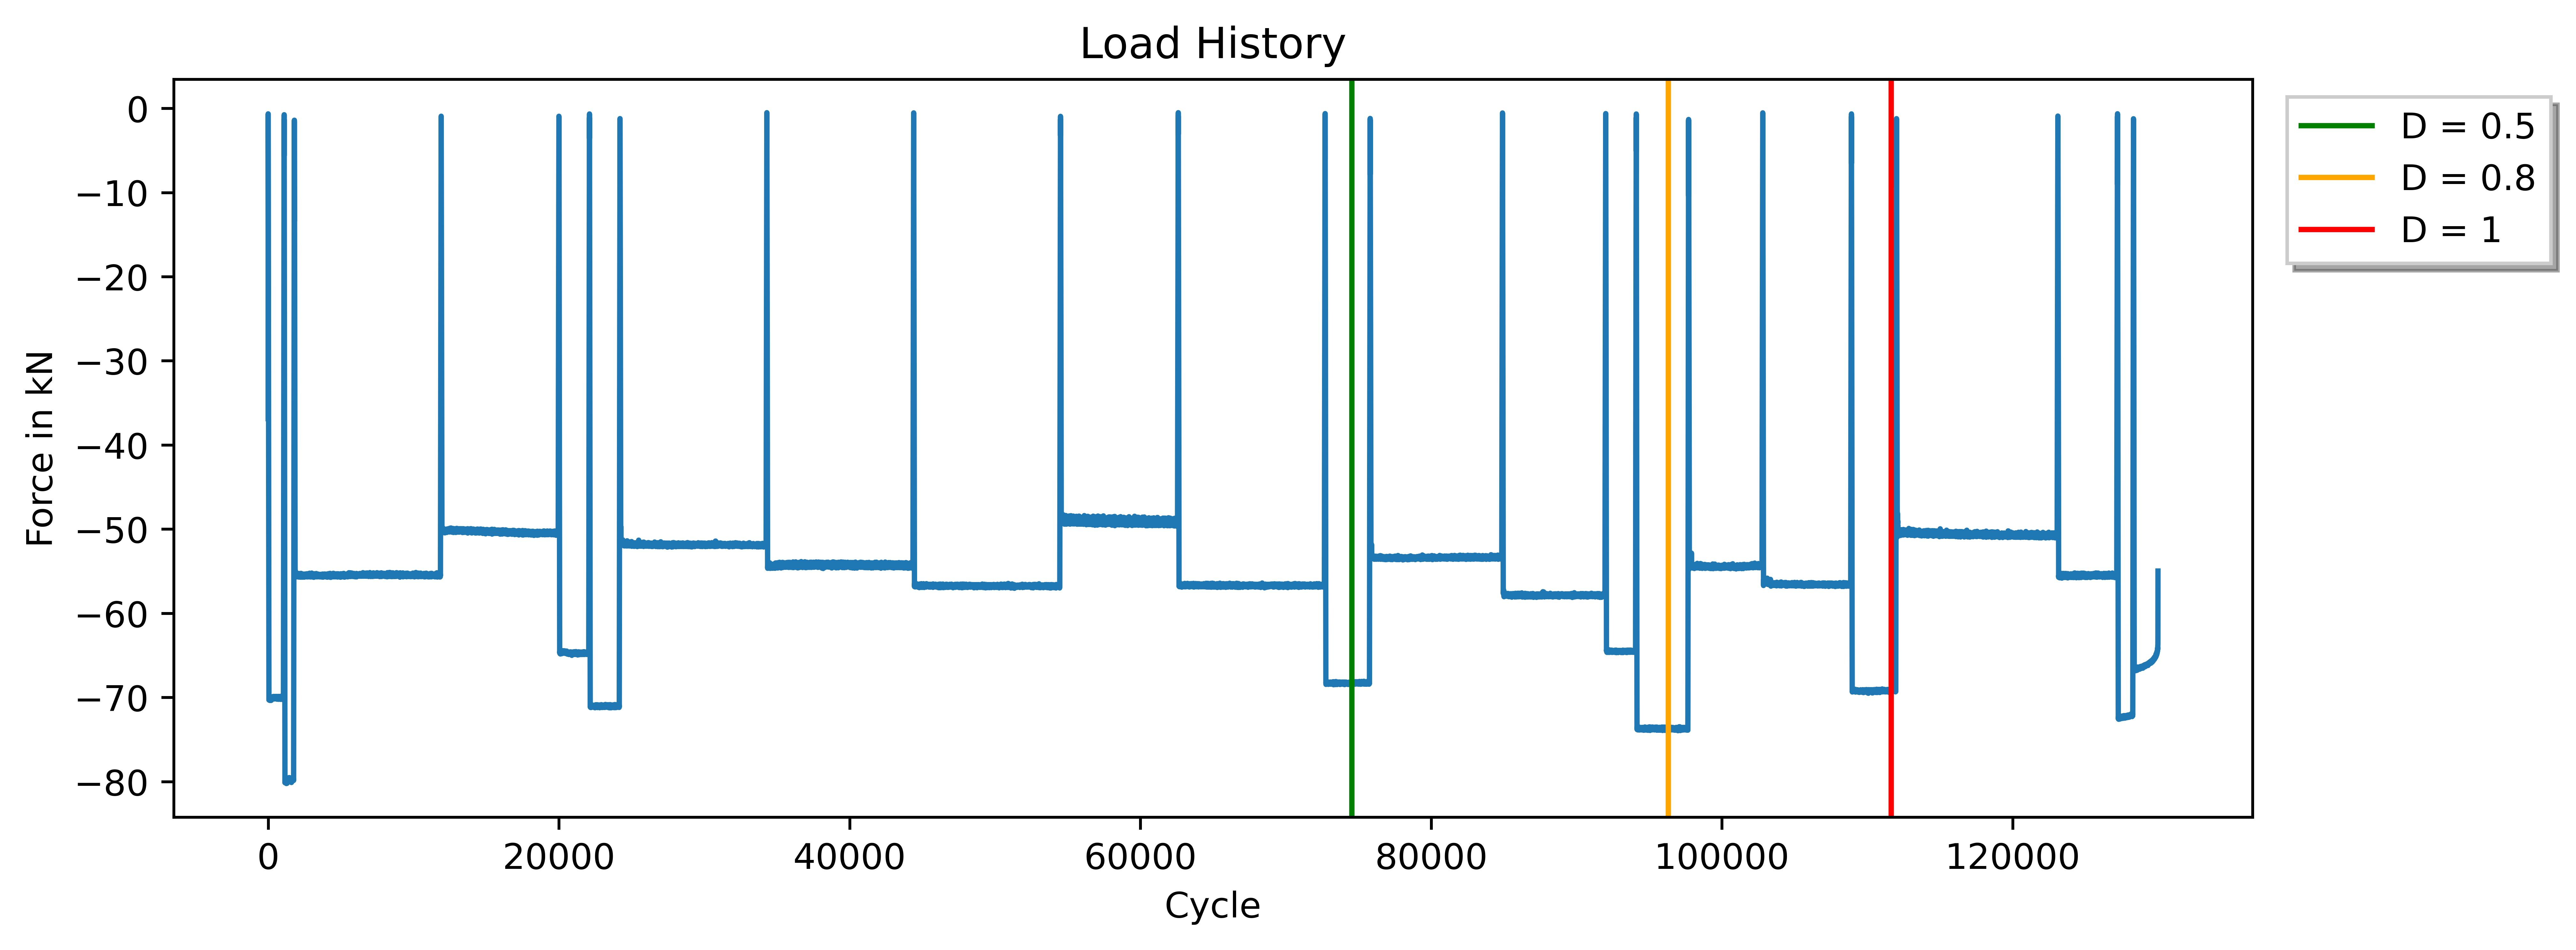
\includegraphics[width=1\linewidth]{IMGs/Load/L1.jpg}
	\caption{Load sequence with failure at D>>1}
	\label{fig:L2}
\end{figure}

\begin{figure}[H]
	\centering
	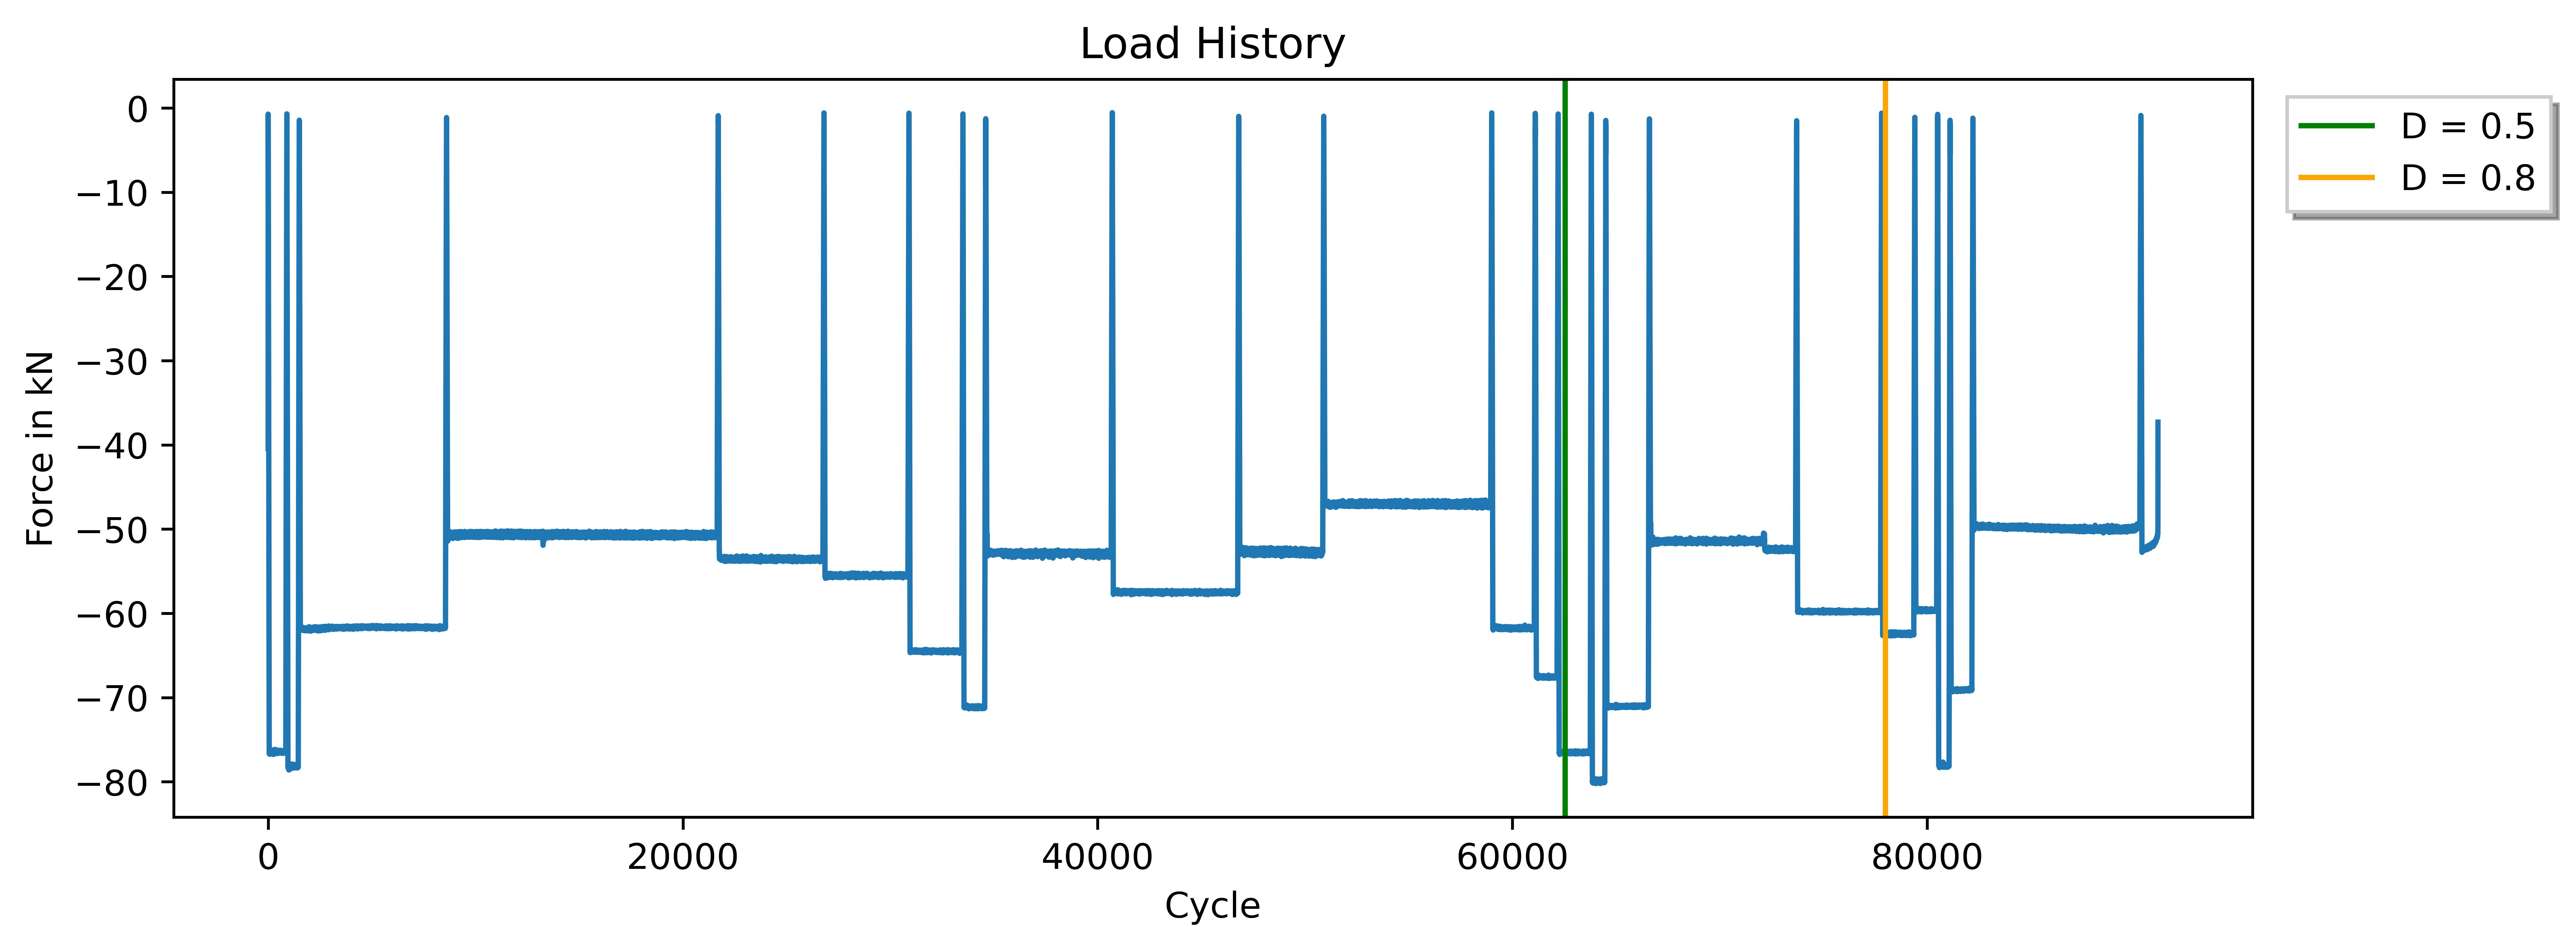
\includegraphics[width=1\linewidth]{IMGs/Load/L2.jpg}
	\caption{Load sequence with failure at D<<1}
	\label{fig:L3}
\end{figure}

Note that the absolute values are irrelevant and can be changed as long as all load sequences are transformed in the same way. Flipping the sign or dividing by a constant to get the stress per unit area will result in equal performance of the selected method.
\newpage
\section{General Overview of the Proposed Structure}\label{GO}
The first goal is to use a classifier to determine if a load sequence will result in early (D<1), late (D>1) or on-time failure (D$\approx$1). In other words, if a load sequence is more or less damaging than assumed by the Miner-Rule, based on the order of the loads. Based on that knowledge, it is possible to deduce the confidence in the damage sum D that was calculated with the Miner rule. For example, if the load sequence is classified as part of the less damaging ones, it is fair to assume that the Miner rule gives a conservative estimate of the actual physical damage. 

After that, a regression is performed to estimate a new defined health indicator called "State of Health" (SOH). 
Figure \ref{fig:GeneralMethod1} shows the process of classifying a load sequence with unknown effects, based on the available load sequences that are used as training data. 

\begin{figure}[H]
	\centering
	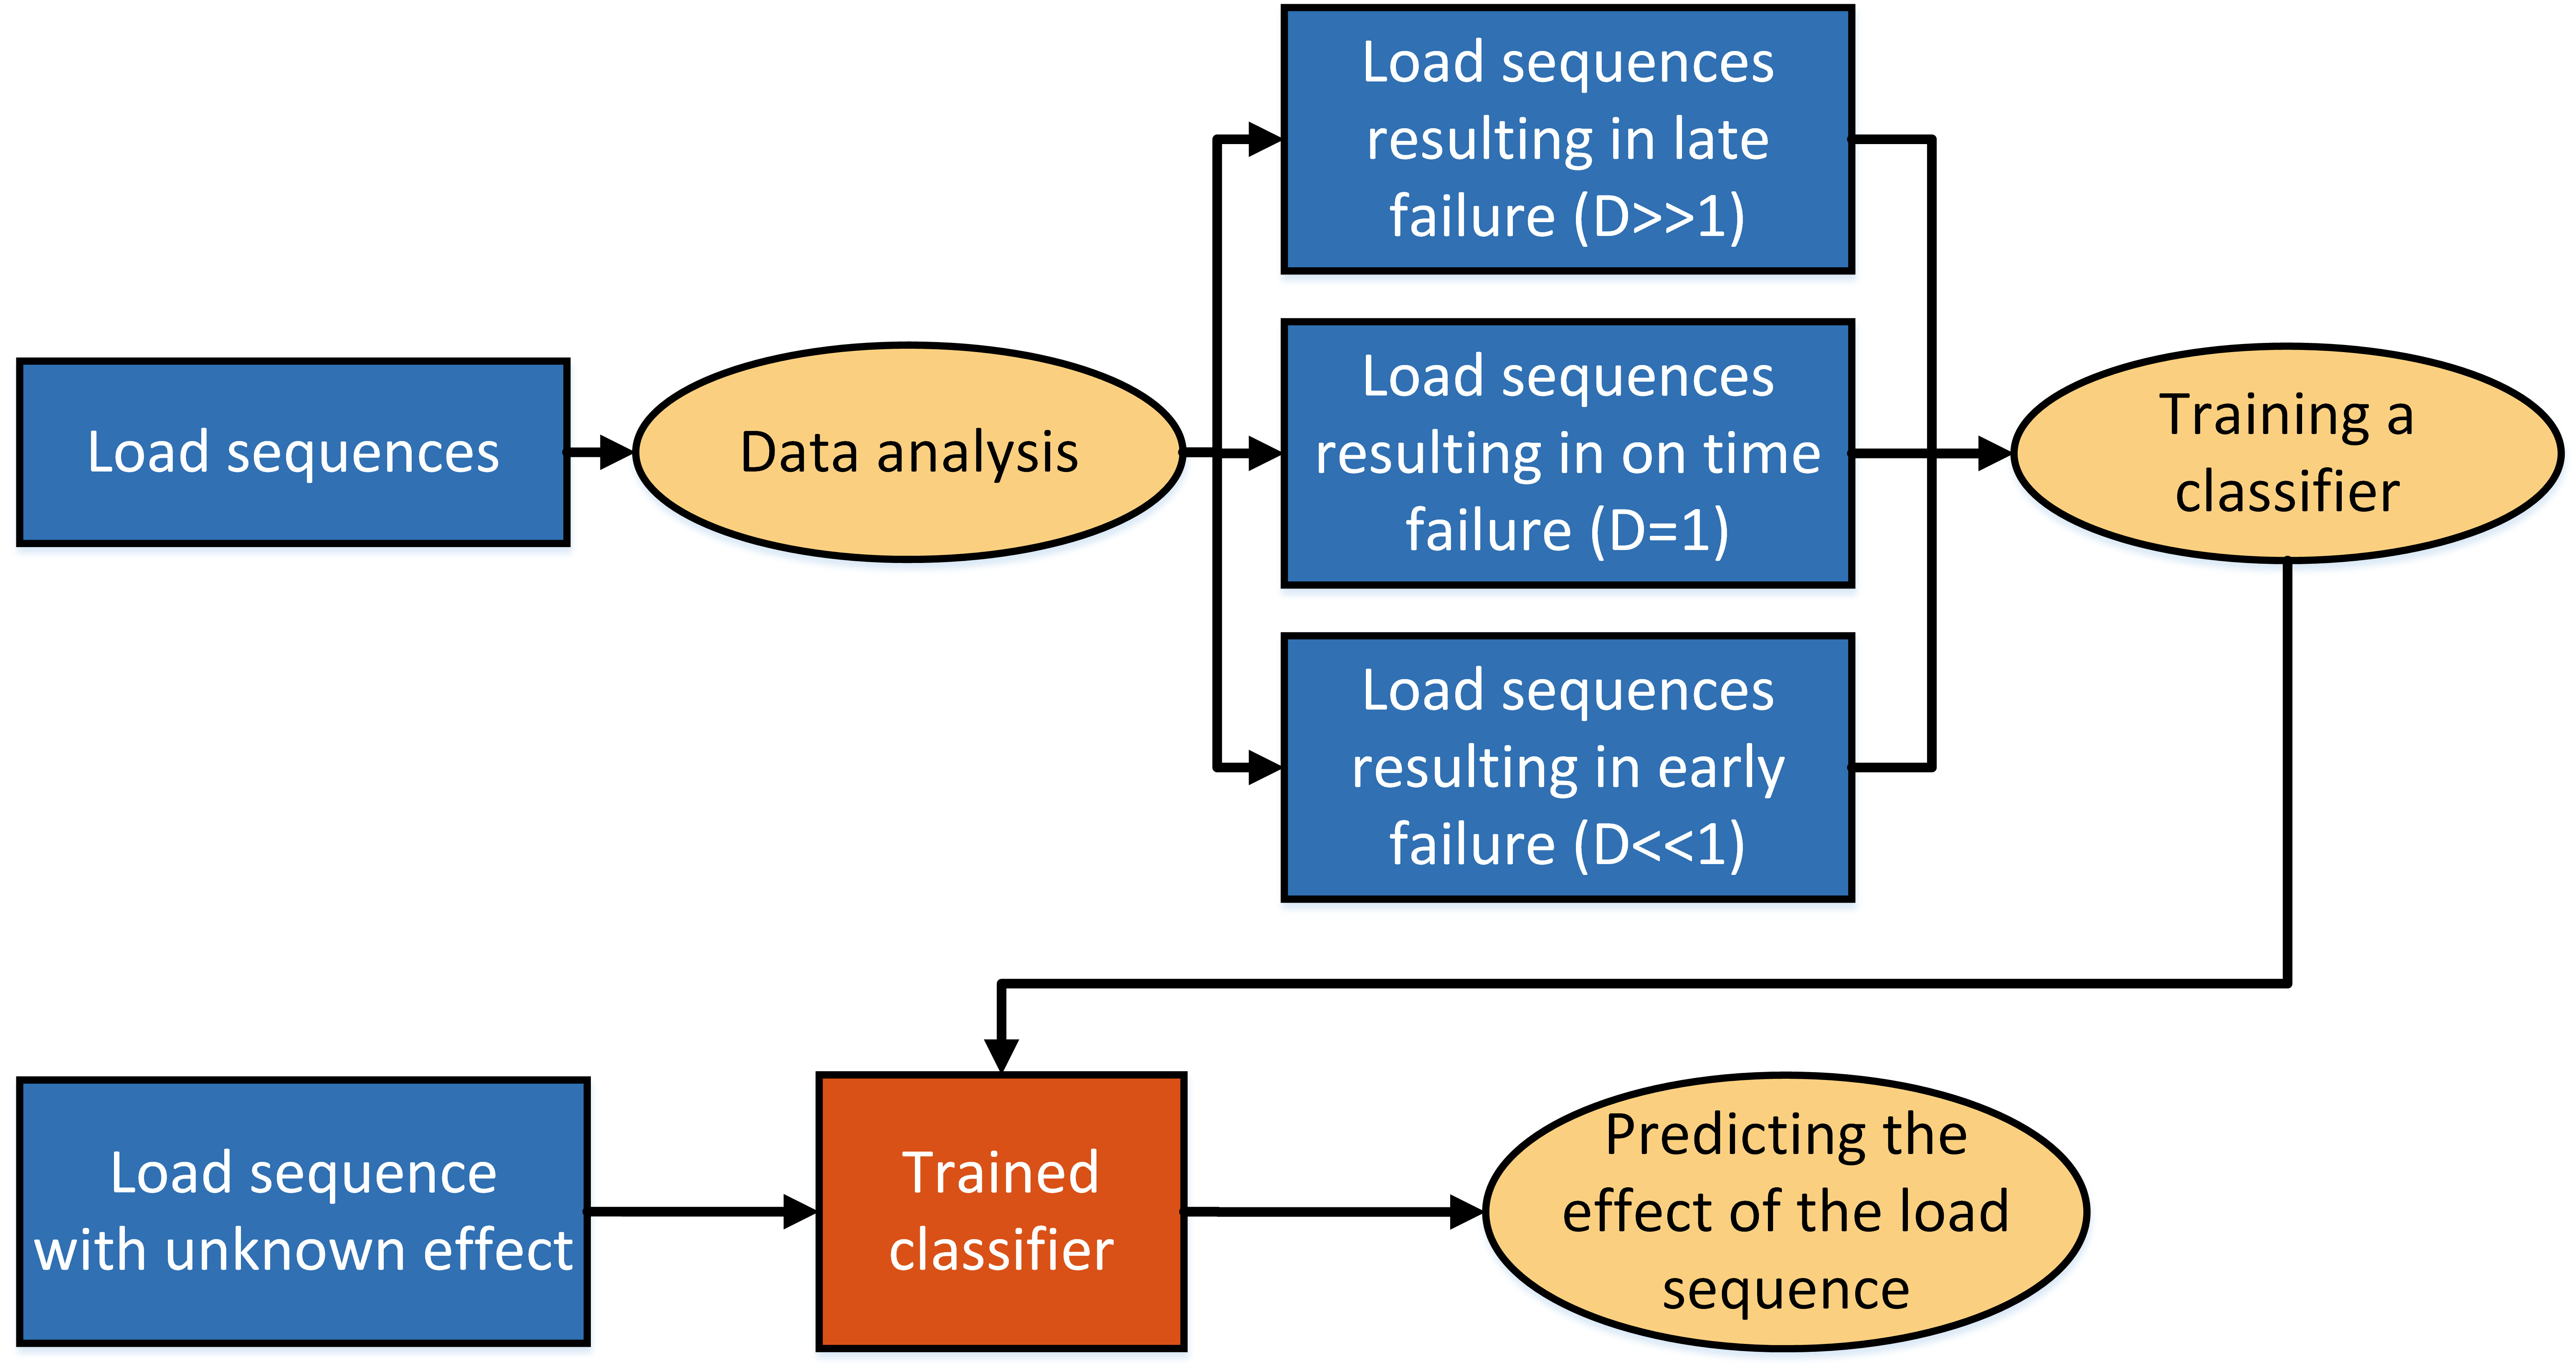
\includegraphics[width=0.95\linewidth]{IMGs/Method1.png}
	\caption{Methodology for classifying a load sequence with unknown effect}
	\label{fig:GeneralMethod1}
\end{figure}

The SOH is not to be confused with a RUL prediction. SOH is comparable to a cars' notification that, for example, the brakes are 80\% worn down and will soon require a maintenance visit to the mechanic. 

The SOH prediction is based on similarly damaging load sequences, with a linear interpolation between the starting point of the sequence at 0, and failure at 1. The damage sum is not taken into account in this step. 
Figure \ref{fig:GeneralMethod2} shows a schematic diagram of how a SOH prediction is acquired.
First, a subset of the original datasets is taken where all load sequences have the same damaging effect. That means that they are either more damaging and thus resulting in early failures, or less damaging, allowing them to run past an accumulated damage sum greater than unity.\newline

The end points of those known sequences are mapped to a linear function starting at 0 at the beginning of the sequence and ending at 1 at the end. This function is referred to as the label-function. The label is the value of the label function at the end of a sequence. Now, the load sequences are cut at different endpoints. The label of the shortened sequences is calculated with the label-function. The shortened sequences and their corresponding labels are combined into a data-set. That data-set is used to train a regressor to predict the SOH of a new sequence. The detailed explanation of the involved steps for predicting the SOH follows in chapter \ref{PrRe}.

Figure \ref{fig:GeneralMethod2} shows a diagram of the proposed structure for the usage of the regressor. 
 
\begin{figure}[H]
	\centering
	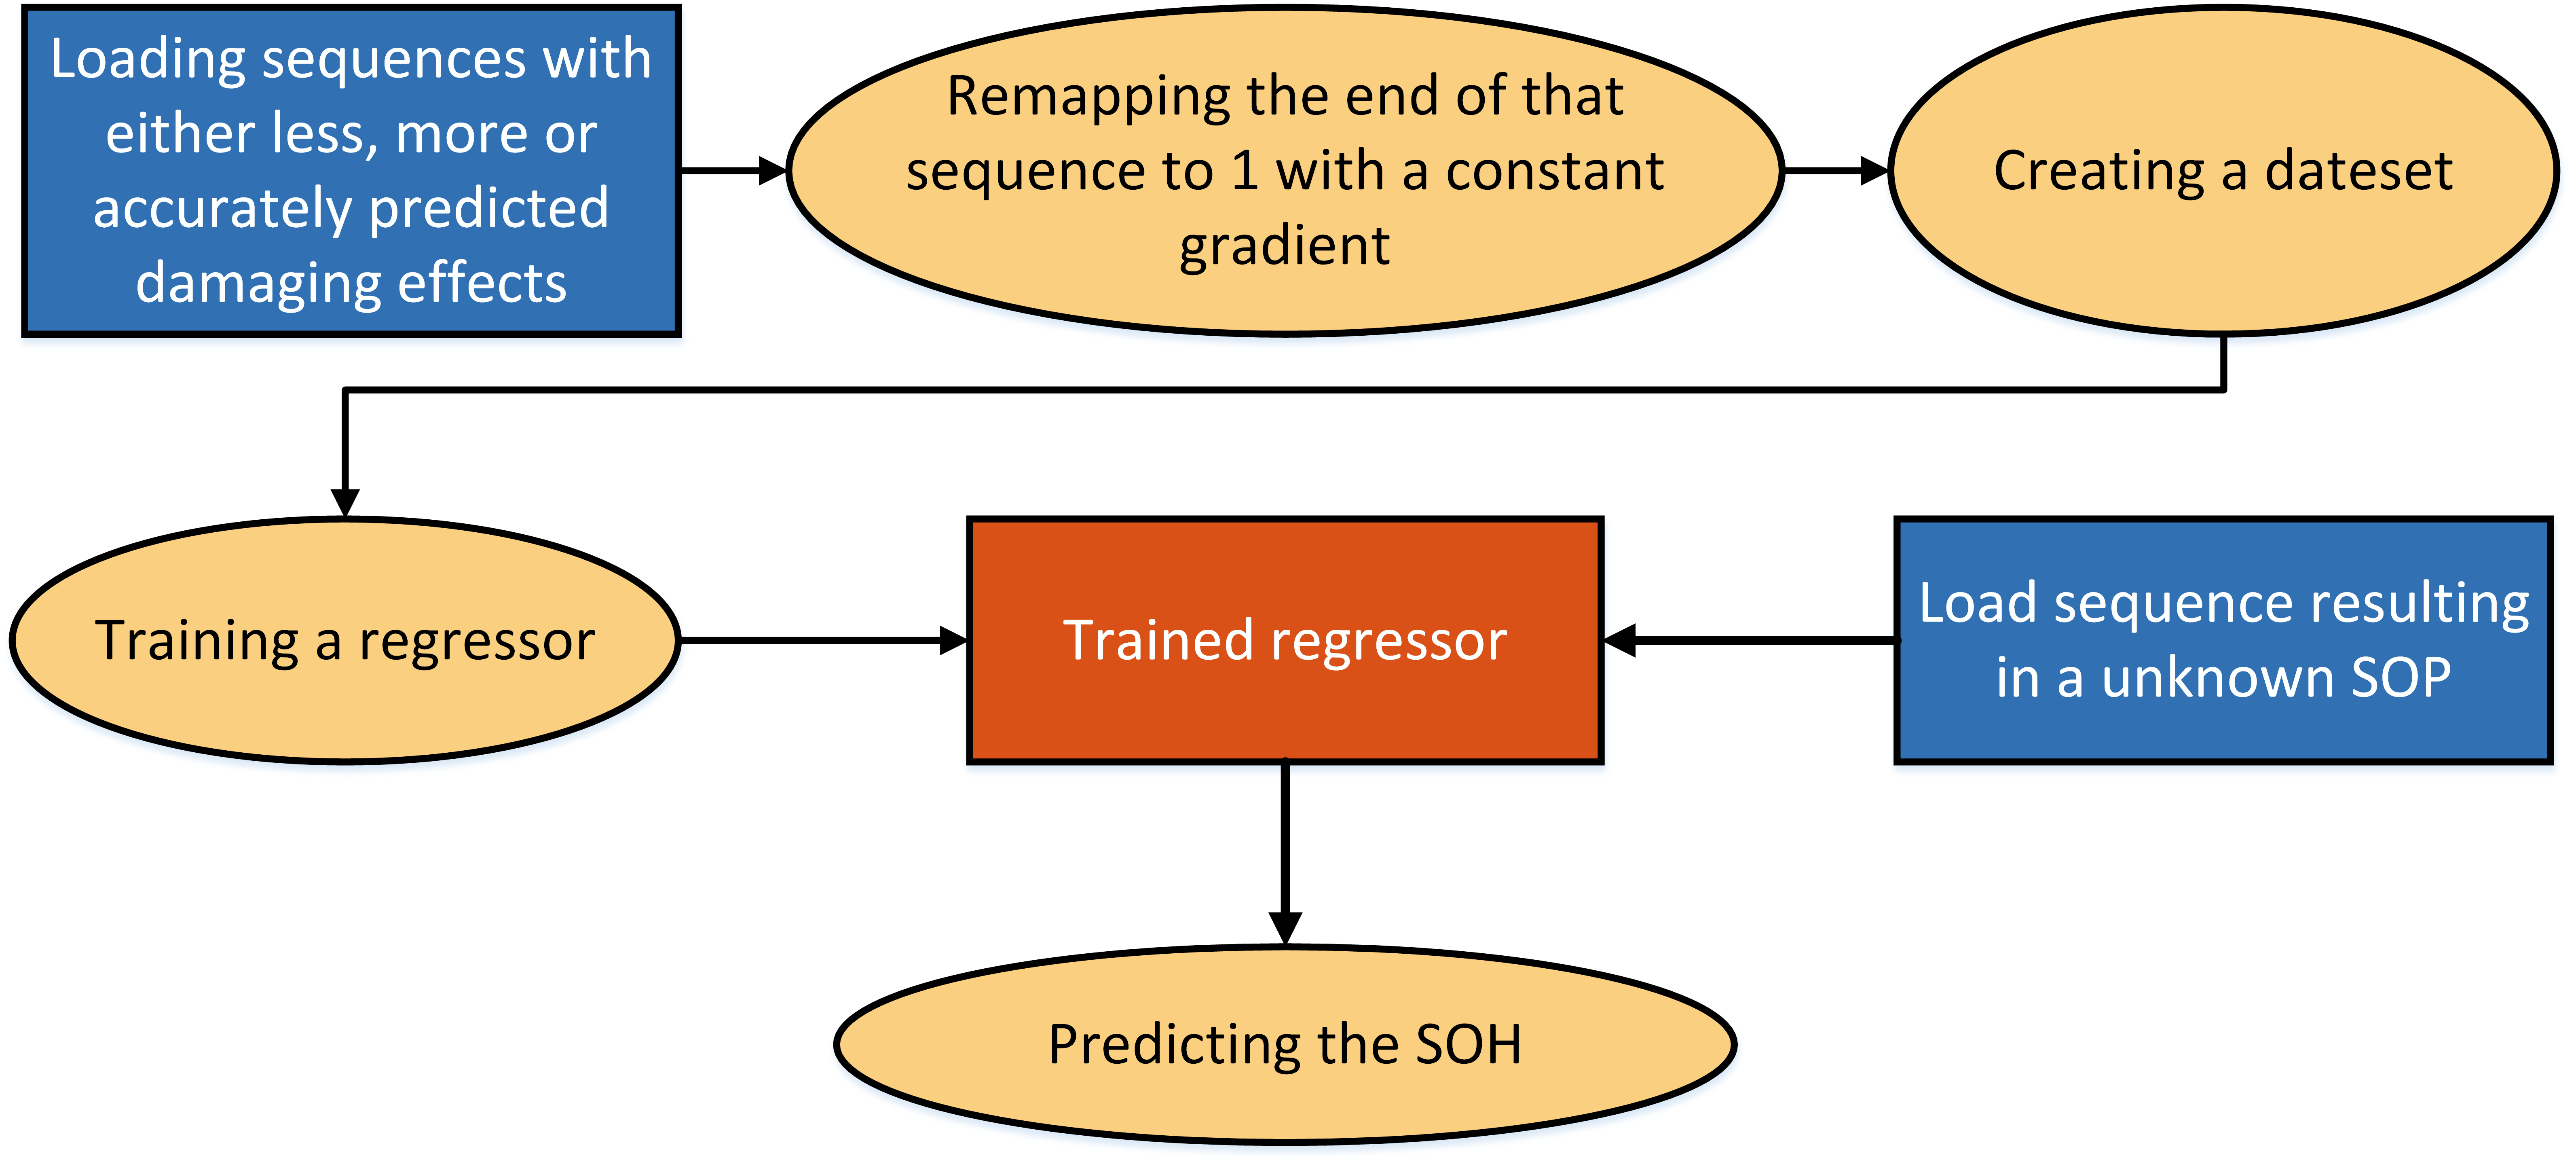
\includegraphics[width=1\linewidth]{IMGs/Method2.png}
	\caption{Methodology for predicting a SOH based on load sequences with similar damaging effects}
	\label{fig:GeneralMethod2}
\end{figure}


In the following, load sequences that have been acquired by STBF are referred to as "finished" load sequences due to the fact that they ended in failure. On the other hand, load sequences that have not yet ended in failure and need to be classified are referred to as "unfinished" load sequences. Only the finished load sequences are used for training the classifier and regressor.
\newpage

\section{Preparation of the Classifier}
\subsection{Separation based on Class Label}\label{SBOC}
When it comes to classification, it requires a data-set that is labeled (see Chapter \ref{SUPER}). The recordings provided by the experiments do not contain any clear indicators from which the label can be deduced right away. To acquire the label for each individual sequence, the Basquin-Equation \cite{DIN50100} has to be utilized. With the help of this equation, shown in equation \ref{BQ}, the maximum load-cycles (\(N\)), that an element can withstand at a specific load, can be calculated.

The parameters \(C\), \(L_a\) and \(-k\) are constants representing the reference value of fatigue strength, the value of the load at one cycle and the slope of the S-N fatigue strength curve \cite{SOLID}. 
\begin{equation}\label{BQ}
	N = {C}*{L_a}^{-k}
\end{equation}
Inputting the result from \ref{BQ} in equation \ref{acc} (from chapter \ref{LAD}) will return the accumulated damage sum D. Figure \ref{fig:SBC} shows the required steps on how the unlabeled load sequences are analyzed and sorted into categories based on the resulting damage sum D. The class labels and according range of damage sum D are shown in table \ref{DamageClass}.

\begin{figure}[H]
	\centering
	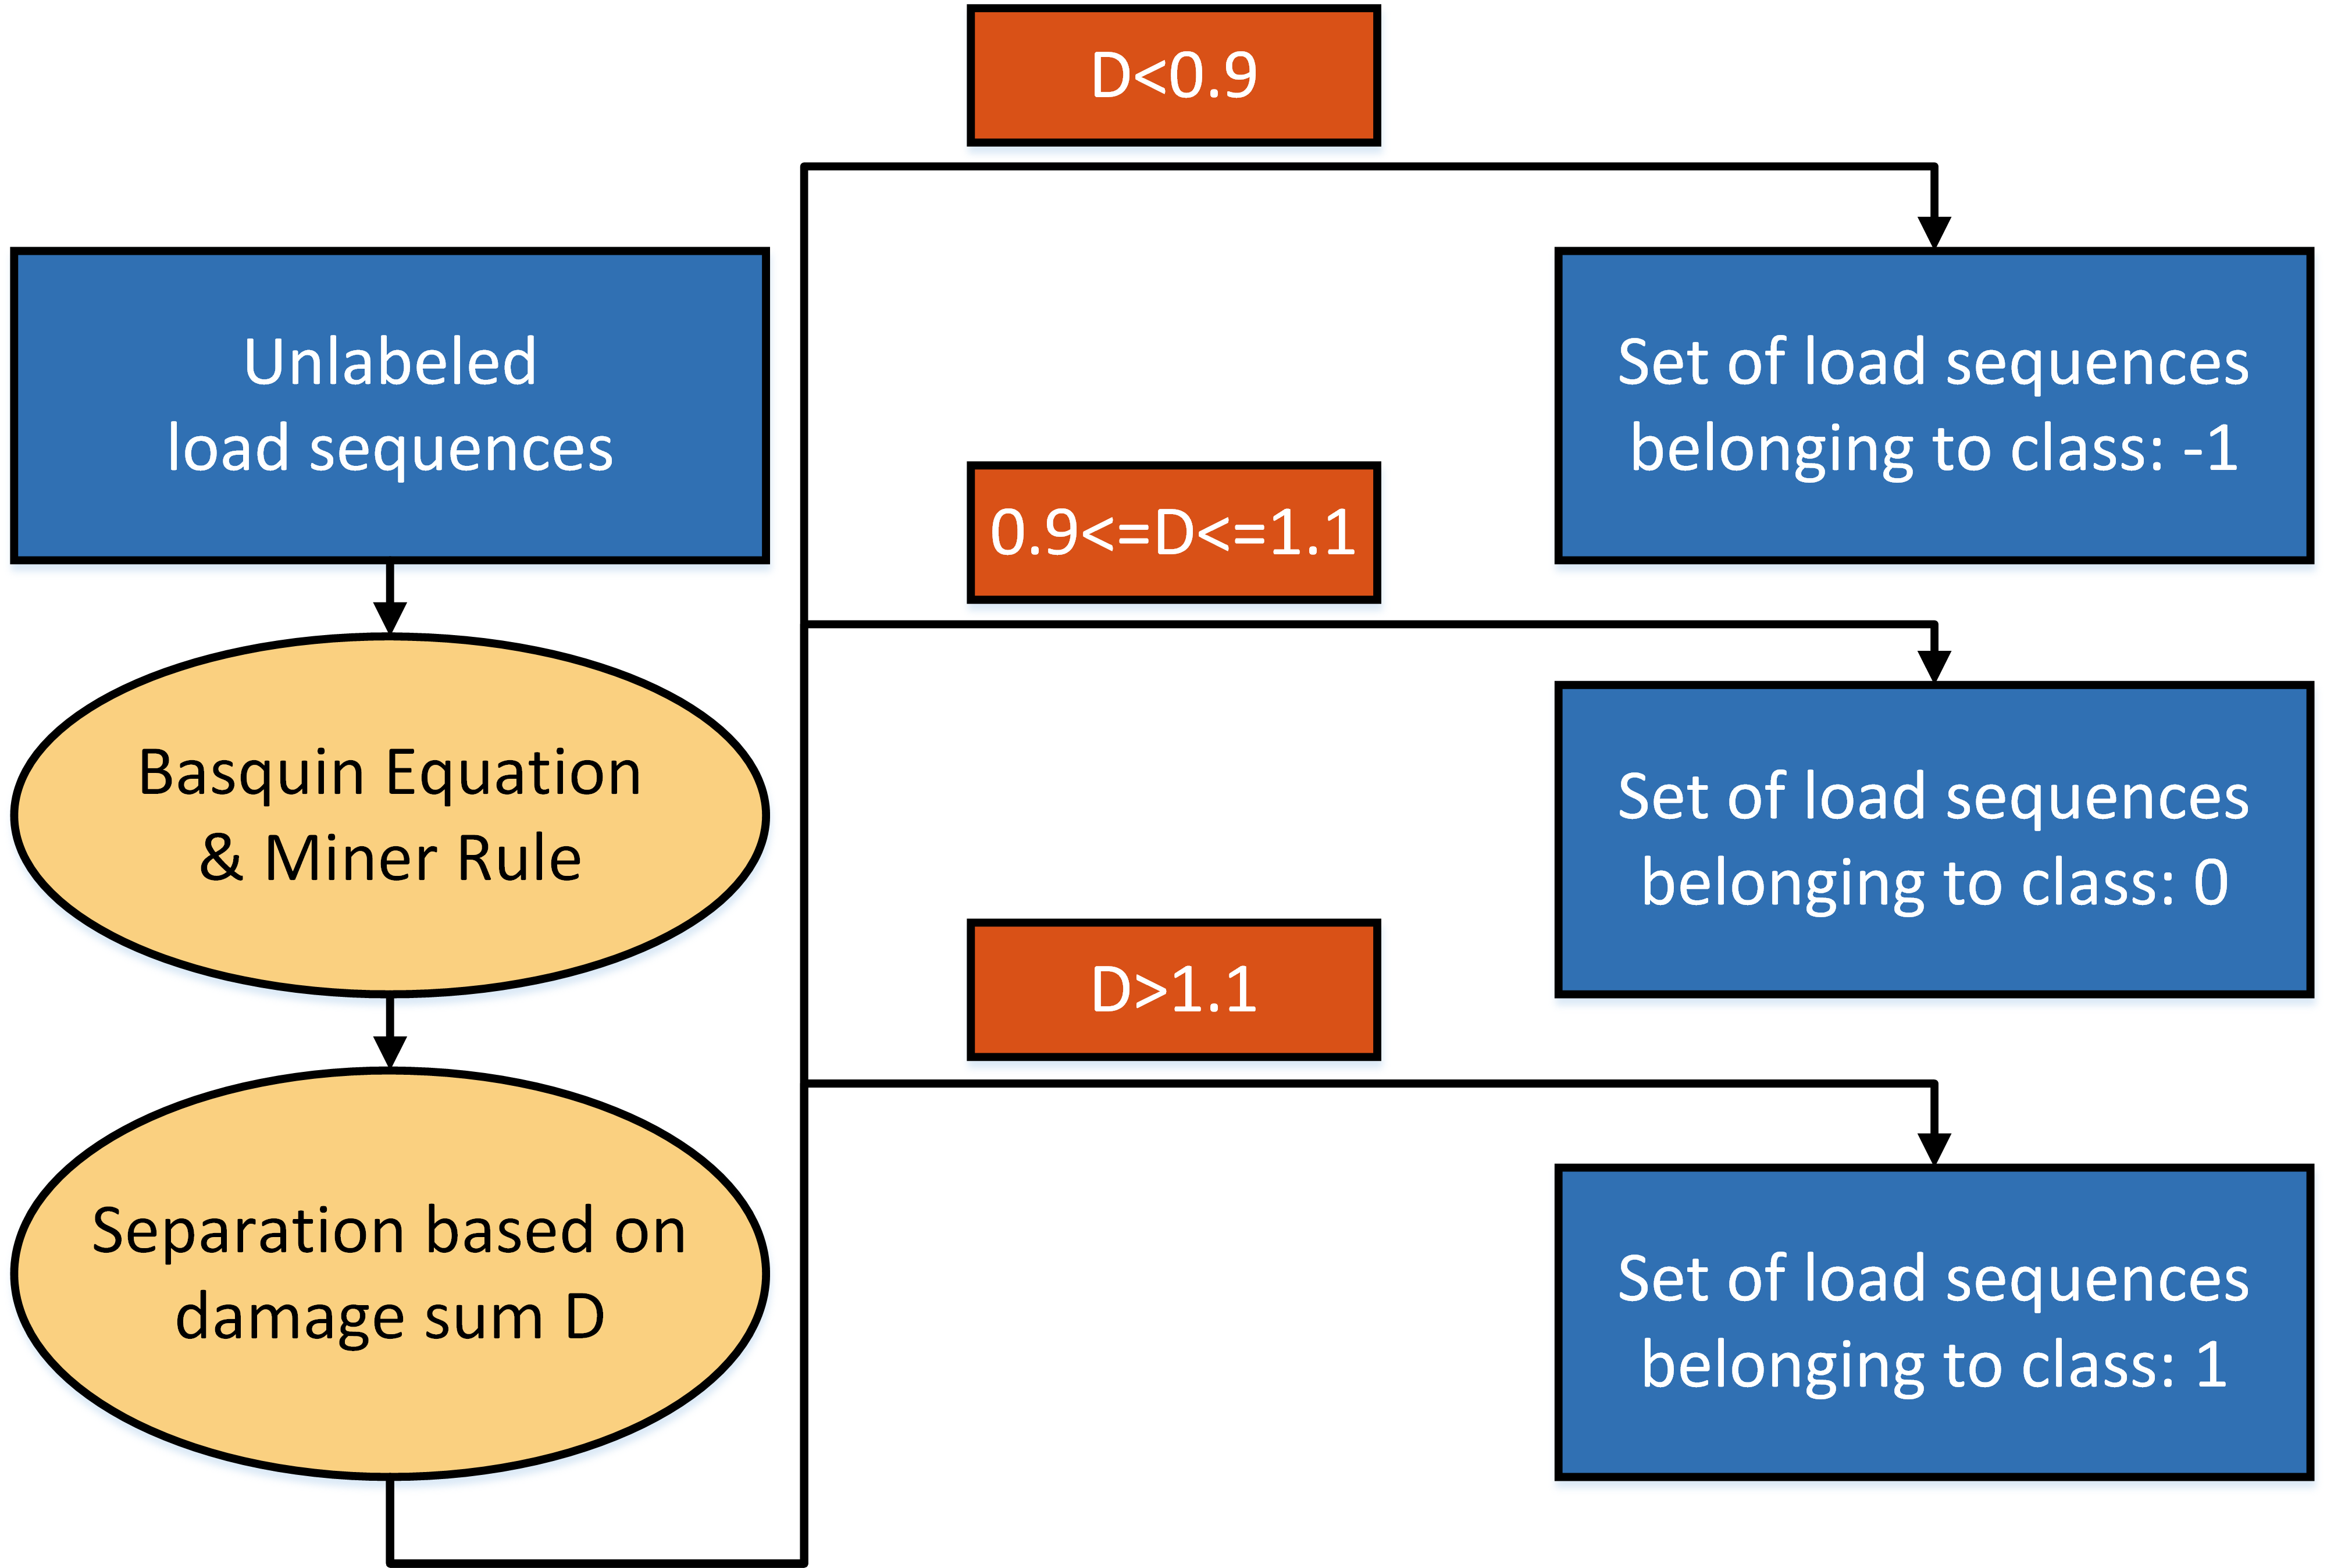
\includegraphics[width=0.8\linewidth]{IMGs/SBC.png}
	\caption{Calculation of damage sum D and separation into classes}
	\label{fig:SBC}
\end{figure}

\begin{table}
	\begin{center}
		\begin{tabular}{|| l | l ||}
			\hline
			\rule{0pt}{2ex}Damage sum D & Class\\
			\hline
			\hline
			\rule{0pt}{2ex}D < 0.9 & Class: -1\\\hline
			0.9 <= D <= 1.1 & Class:  0\\	\hline
			D > 1.1 & Class:  1\\\hline
			\hline
		\end{tabular}
		\caption{Label assignment based on damage sum D}
		\label{DamageClass}
	\end{center}
	\vspace{-4mm}
\end{table}

\newpage
Figure \ref{fig:SBC1} gives a more visual representation of how the different load sequences are separated into classes. Note that short sequences can have a higher damage sum D as it is not dependent on just the number of cycles but also on the load level. The end of a sequence is that point where the gear failed. 

\begin{figure}[H]
	\centering
	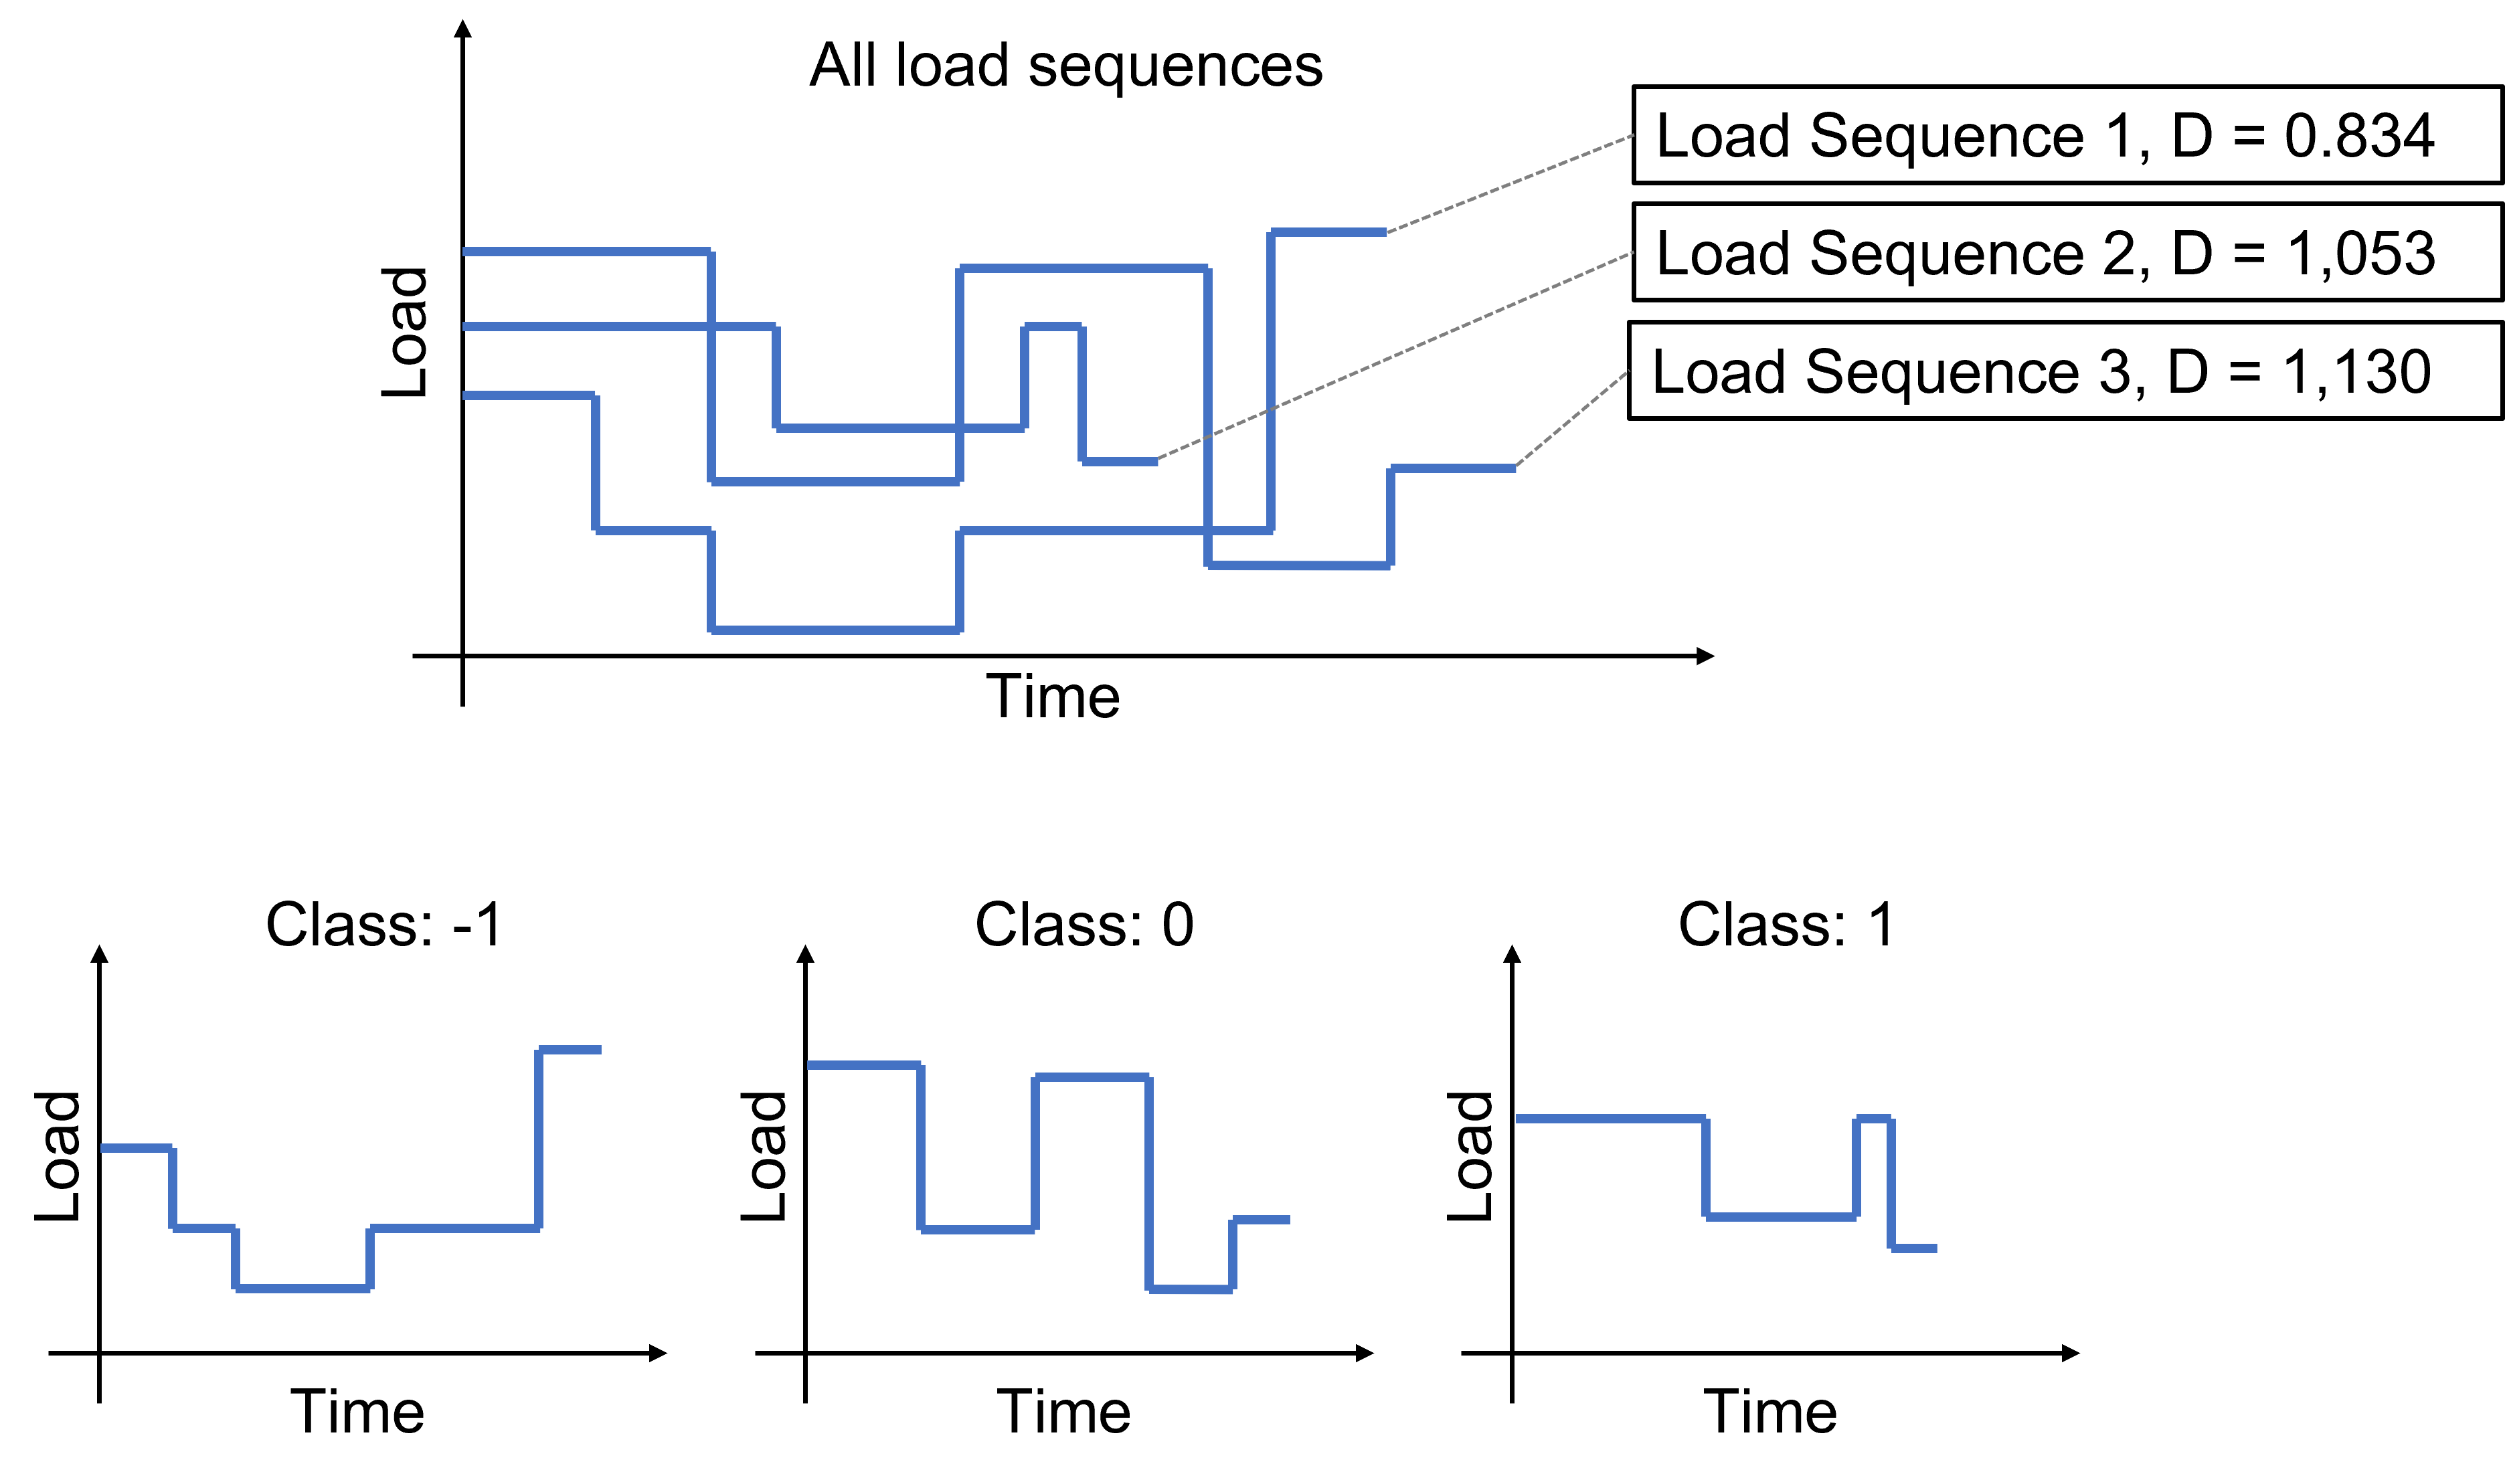
\includegraphics[width=0.9\linewidth]{IMGs/SBC1.png}
	\caption{Separation of load sequences based on classes}
	\label{fig:SBC1}
\end{figure}

\subsection{Pre-processing for Classification}\label{prep_class}
Before the classifier can be trained, further pre-processing steps need to be performed. The first is data augmentation (DA), and the second is dimensionality reduction. 

The goal of DA, as mentioned in chapter \ref{DAUG}, is to increase the diversity and size of a data-set. This gives the classifier more data to train on and reduces the risk of over-fitting.
This step is especially important if the sample size is small. Due to the physical nature of the problem, multiple aspects have to be considered when performing DA.

If the data-set is very limited, DA will only slightly boost the performance, as the inherent problem is the lack of data. Further, if DA is performed, the accumulated damage sum D of the total load sequence must not change significantly. If a load sequence is changed significantly and in a such way the damage sum D is also changed, the inherit properties of the load sequence can be lost. The classifier relies on characteristics that correlate to the label of a load sequence. Significantly changed characteristics will confuse the classifier in training and lead to worse performance.


The same principle applies to the step of dimensionality reduction. ML models perform better with input vectors that are short and have values in a similar range. One possible option for dimensionality reduction is selecting every \(n^{th}\) point in a sequence.
When analyzing, if the reduced sequence has the same damage sum D as the original, the numerator of the Miner rule must be multiplied by the step-size that was used to select every \(n^{th}\) point. For example, if every 200\(^{th}\) point is selected, the step-size is 200. When calculating the damage sum D on the reduced sequence with equation \ref{acc} the numerator must be multiplied by 200.


Figure \ref{fig:DAUG} shows the steps of DA and dimensionality reduction, including a feedback loop to ensure that the augmentation and dimension reduction do not change the damage sum D.
It is important that the comparison is performed after each individual step. In a worst-case scenario, the augmentation and dimensionality reduction change the damage sum in opposite directions. In this case, the final damage sum is equal to the original load sequence, but the characteristics are all lost.

 
\begin{figure}[H]
	\centering
	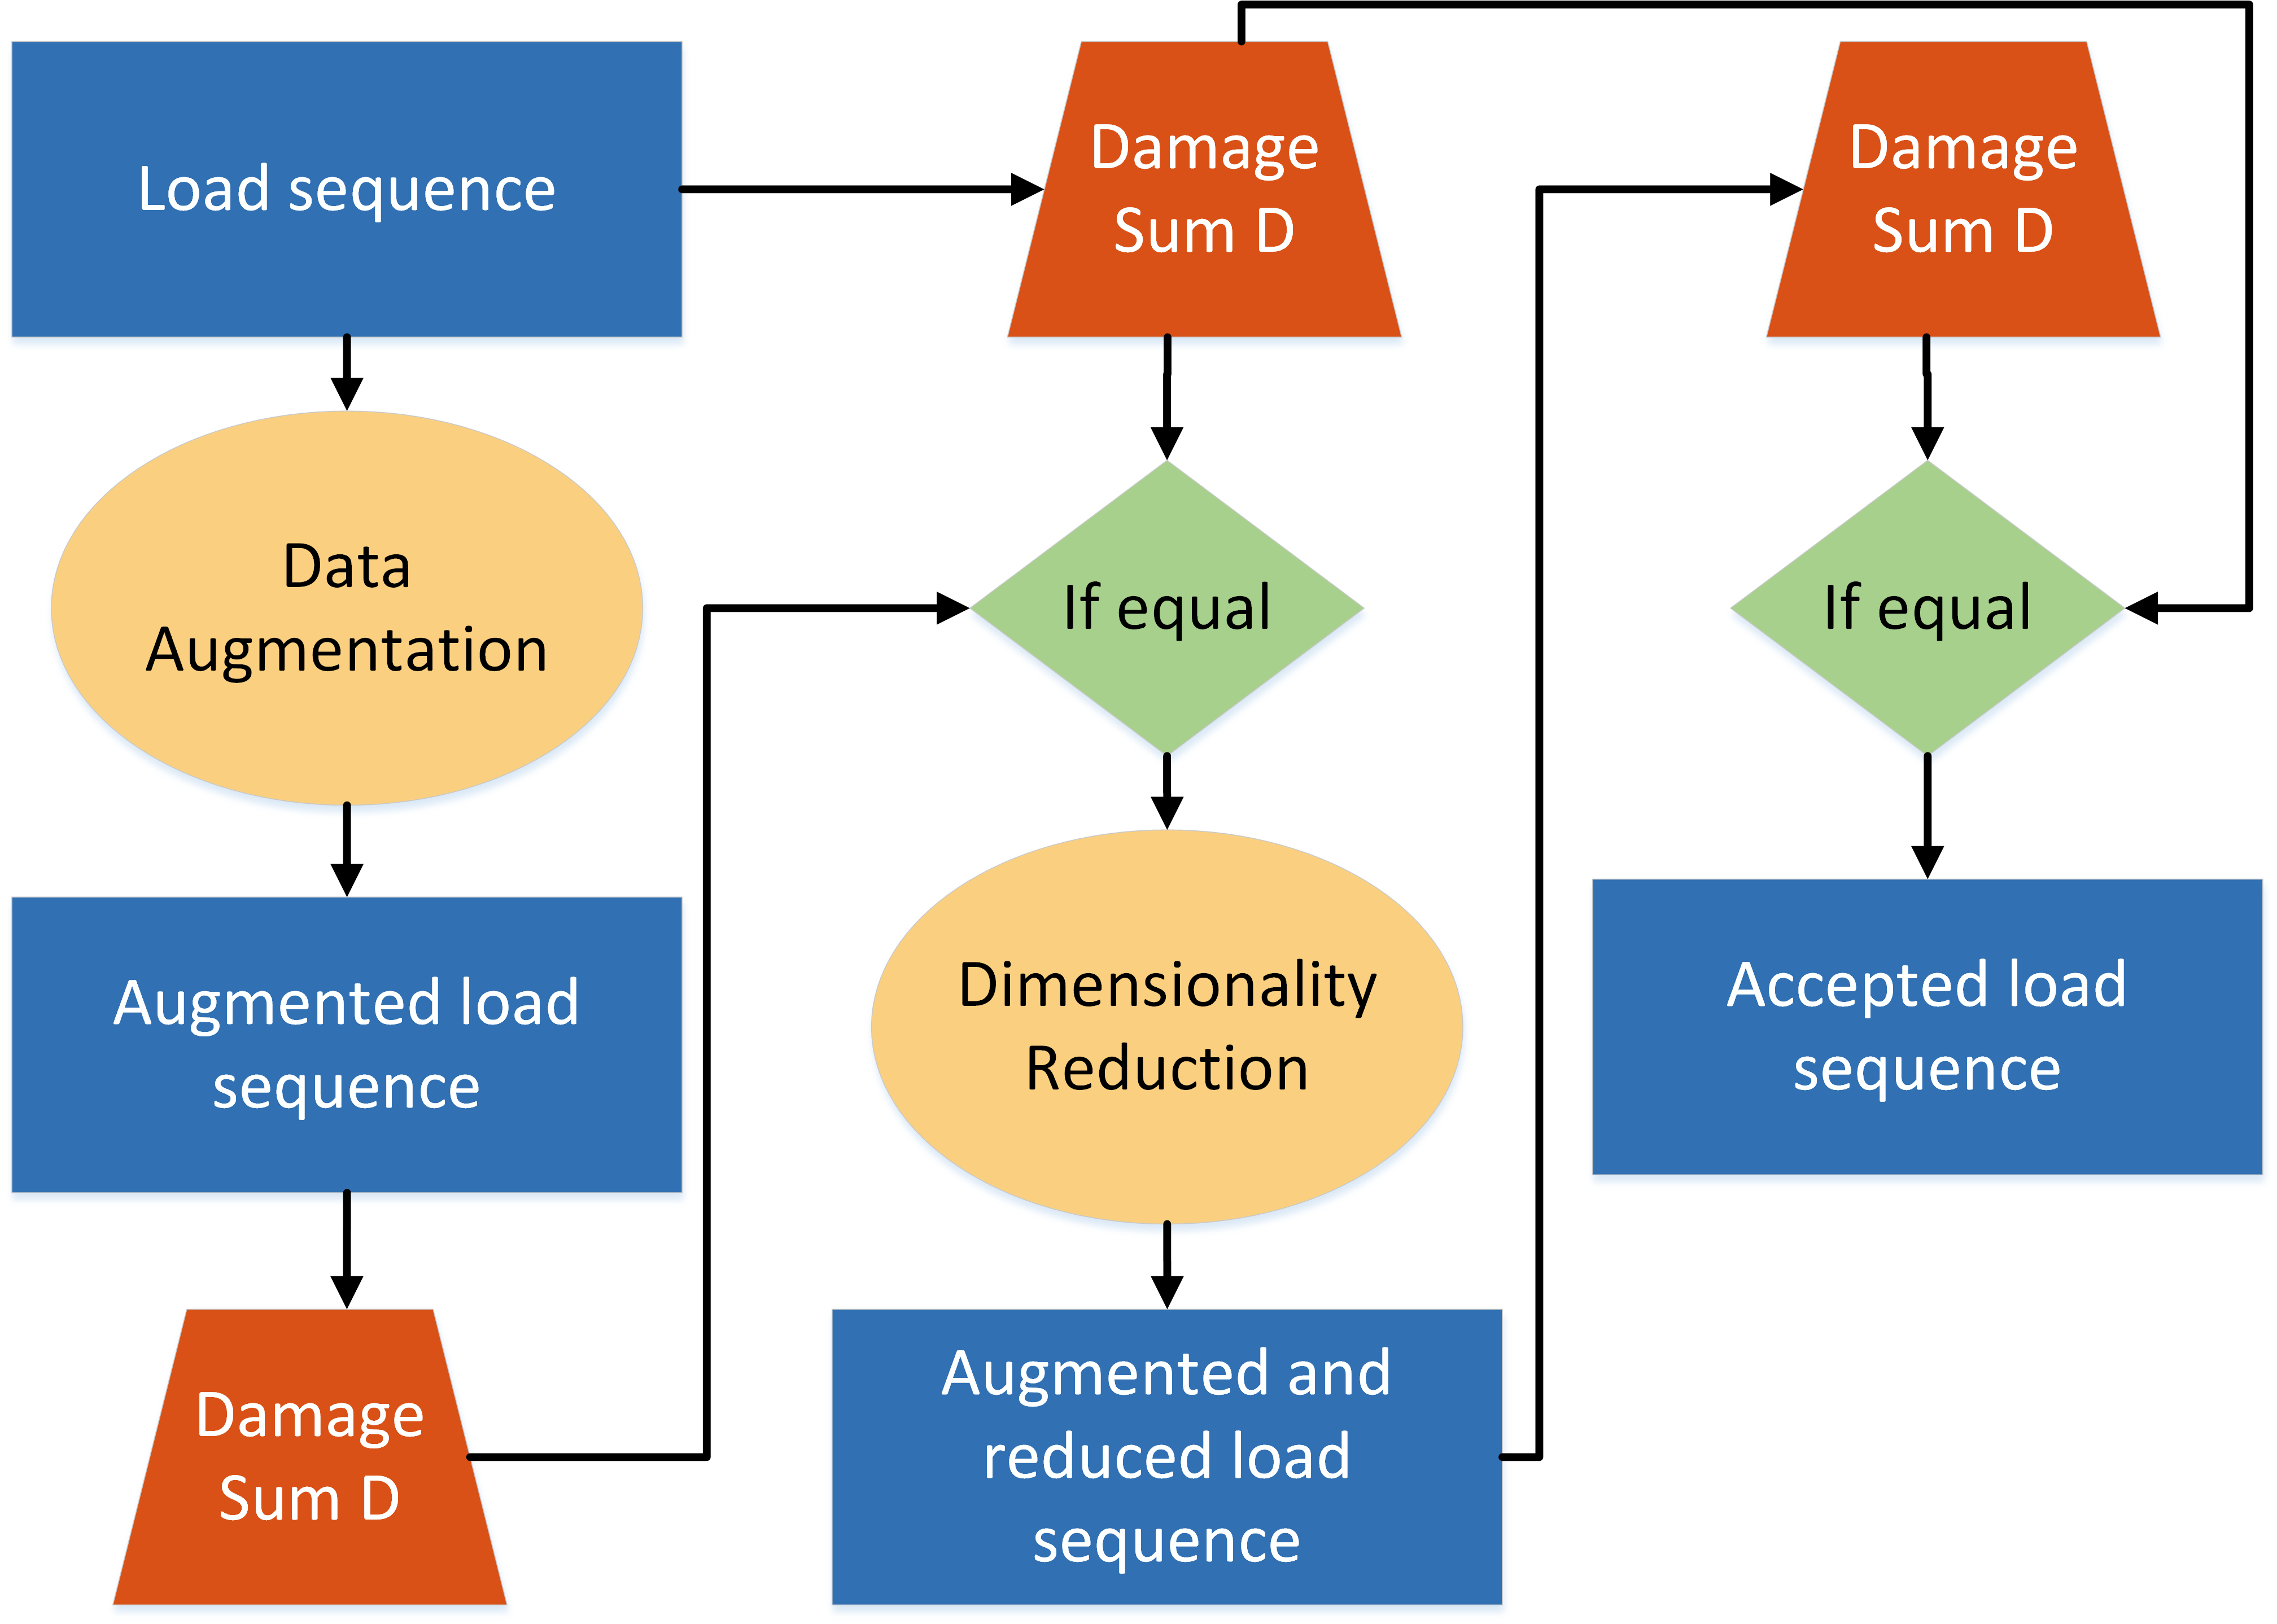
\includegraphics[width=0.8\linewidth]{IMGs/DAUG.png}
	\caption{Data Augmentation and Dimensionality Reduction with feedback loops}
	\label{fig:DAUG}
\end{figure}


Figure \ref{fig:UL} shows the issue of just selecting every \(n^{th}\) point for dimensionality reduction. By missing significant portions of the load sequence, peaks and low spots can be missed or accentuated. Multiplying the number of cycles in the Miner rule with \(n\), is the same as expanding every cycle by \(n\) and using the Miner rule without multiplication. The two graphs in \ref{fig:UL} show that the expanded load sequence has significant differences and all characteristics have been lost. By comparing the damage sum at each step to the original, such cases can be found and not taken into the training data-set. Another way of reducing this problem, is to select a smaller step-size which in turn will increase the feature vector size that will be used as an input.  

\begin{figure}[H]
	\centering
	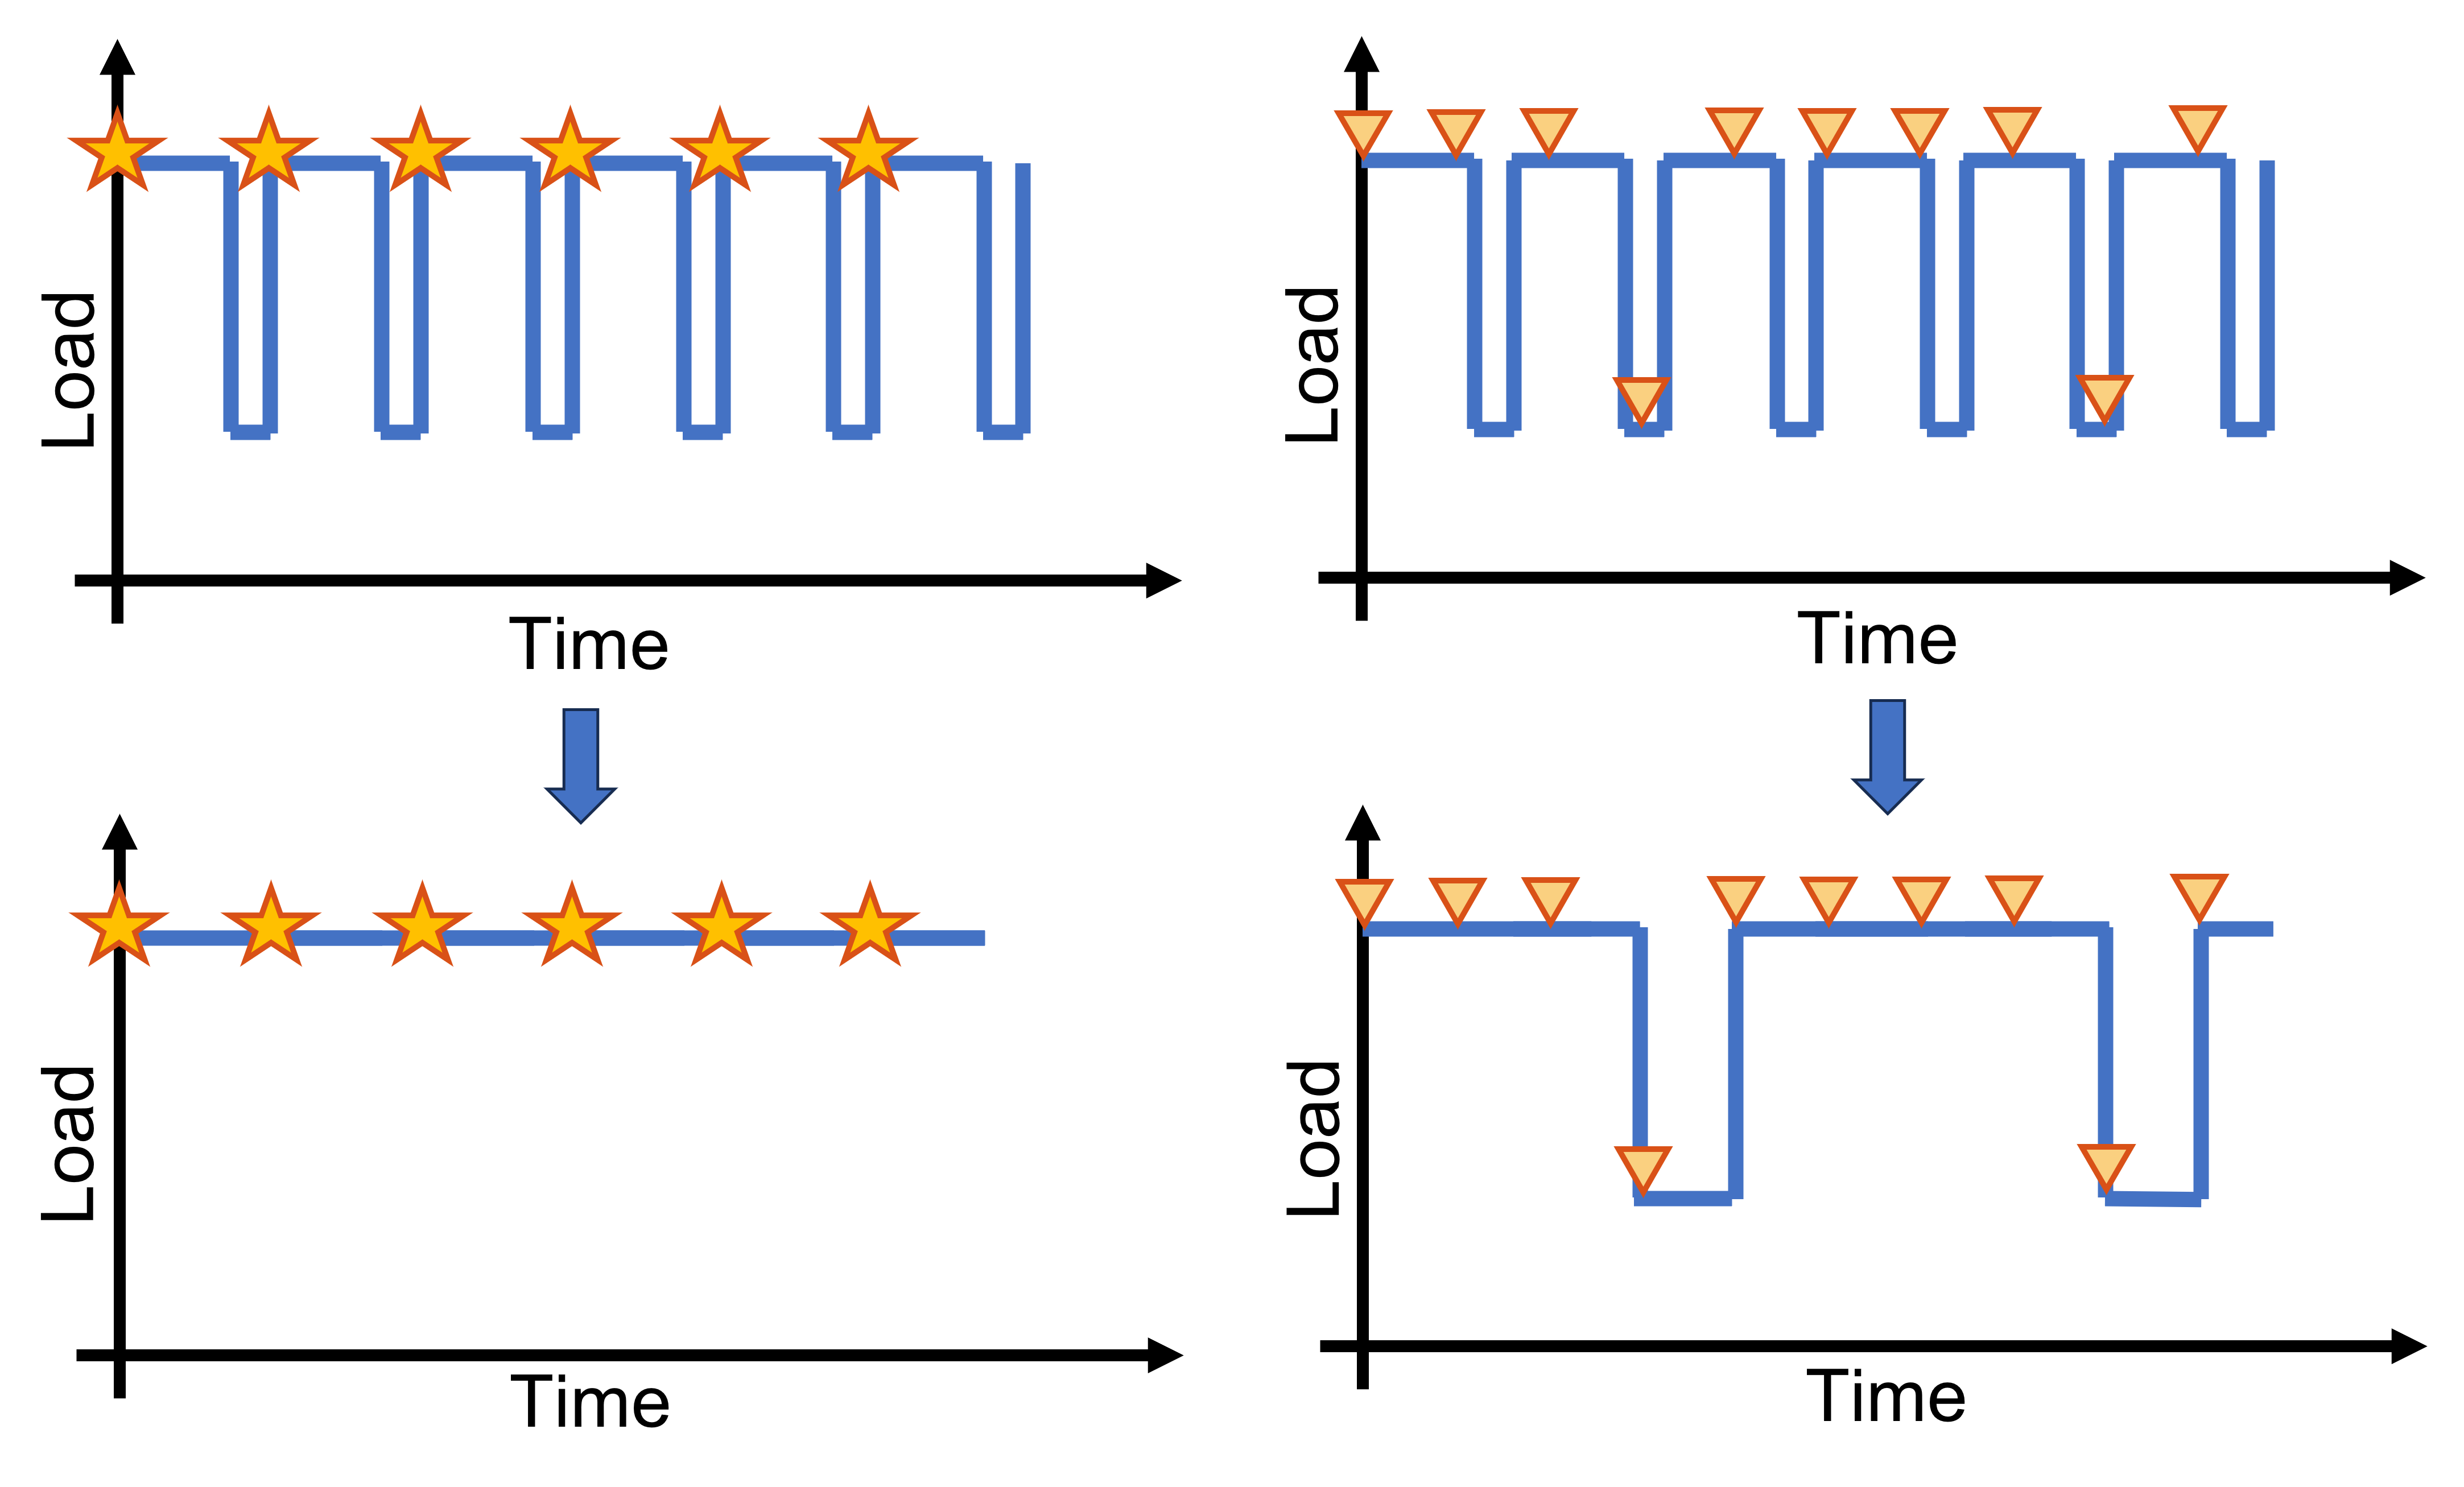
\includegraphics[width=0.8\linewidth]{IMGs/Unlucky.png}
	\caption{Danger of Dimensionality Reduction by selecting equidistant points}
	\label{fig:UL}
\end{figure}
 
\subsection{Usage of the Classifier}
The classifier is used as a method to classify an unfinished load sequence, whether it is part of the more damaging or less damaging ones. After the performed steps of separation into classes, DA and dimensionality reduction, the load sequences require a last pre-processing step. At the moment, the load sequences are in their full length and have a different damage sum D.
If an unfinished sequence, of a gear that has not yet suffered fatigue damage, needs to be classified, the comparison has to be made with sequences that have the same damage sum D as the unclassified sequence. In other words, if a current sequence is at damage sum D = 0.6 and it is of interest if this is a correct estimate, it needs to be compared to other load sequences at D = 0.6.
 
To do so, all sequences are cut (shortened) so that they all end at the same damage sum D. 
With those sequences and their labels, the classifier is trained.
After training, the classifier can take the unfinished sequence, that underwent the same dimensionality reduction as the rest, and predict a class-label. 
Based on the predicted class label, a conclusion can be drawn if the calculated damage sum D based on the Miner rule is more on the conservative or lenient side. Figure \ref{fig:Class} shows the steps of the last pre-processing steps and the classification of a sequence.


\begin{figure}[H]
	\centering
	\includegraphics[width=0.9\linewidth]{IMGs/Class.png}
	\caption{Load sequence adaption, training and final classification }
	\label{fig:Class}
\end{figure}


Figure \ref{fig:Shortened} gives a visual representation of how load sequences of class 1 (D>1.1) are adapted when the unfinished sequence has the damage sum D of 0.6 according to the Miner rule.
All recorded points after D=0.6 are deleted in every load sequence. By doing so, the sequences are shortened. These sequences are then used as training data to predict the label of the unlabeled sequence. The same is done to the sequences of classes 0 and 1.

Note that if an unlabeled sequence it past a certain damage sum D, the classification will become more uncertain. For example if a sequence has a damage sum D = 0.85 but most of the sequences in class -1 end at 0.8, there are significantly fewer data samples that can be used for training in that class. 

For a classification of a load sequence that has a very low damage sum D (for example 0.3) the classification also becomes very uncertain, as it is possible that not enough characteristics are present in a load sequence that could place it in one category with high certainty.
So there exists a sweet-spot that is determined by the number of training-elements in class -1 and the damage sum D of the unknown label.

\begin{figure}[H]
	\centering
	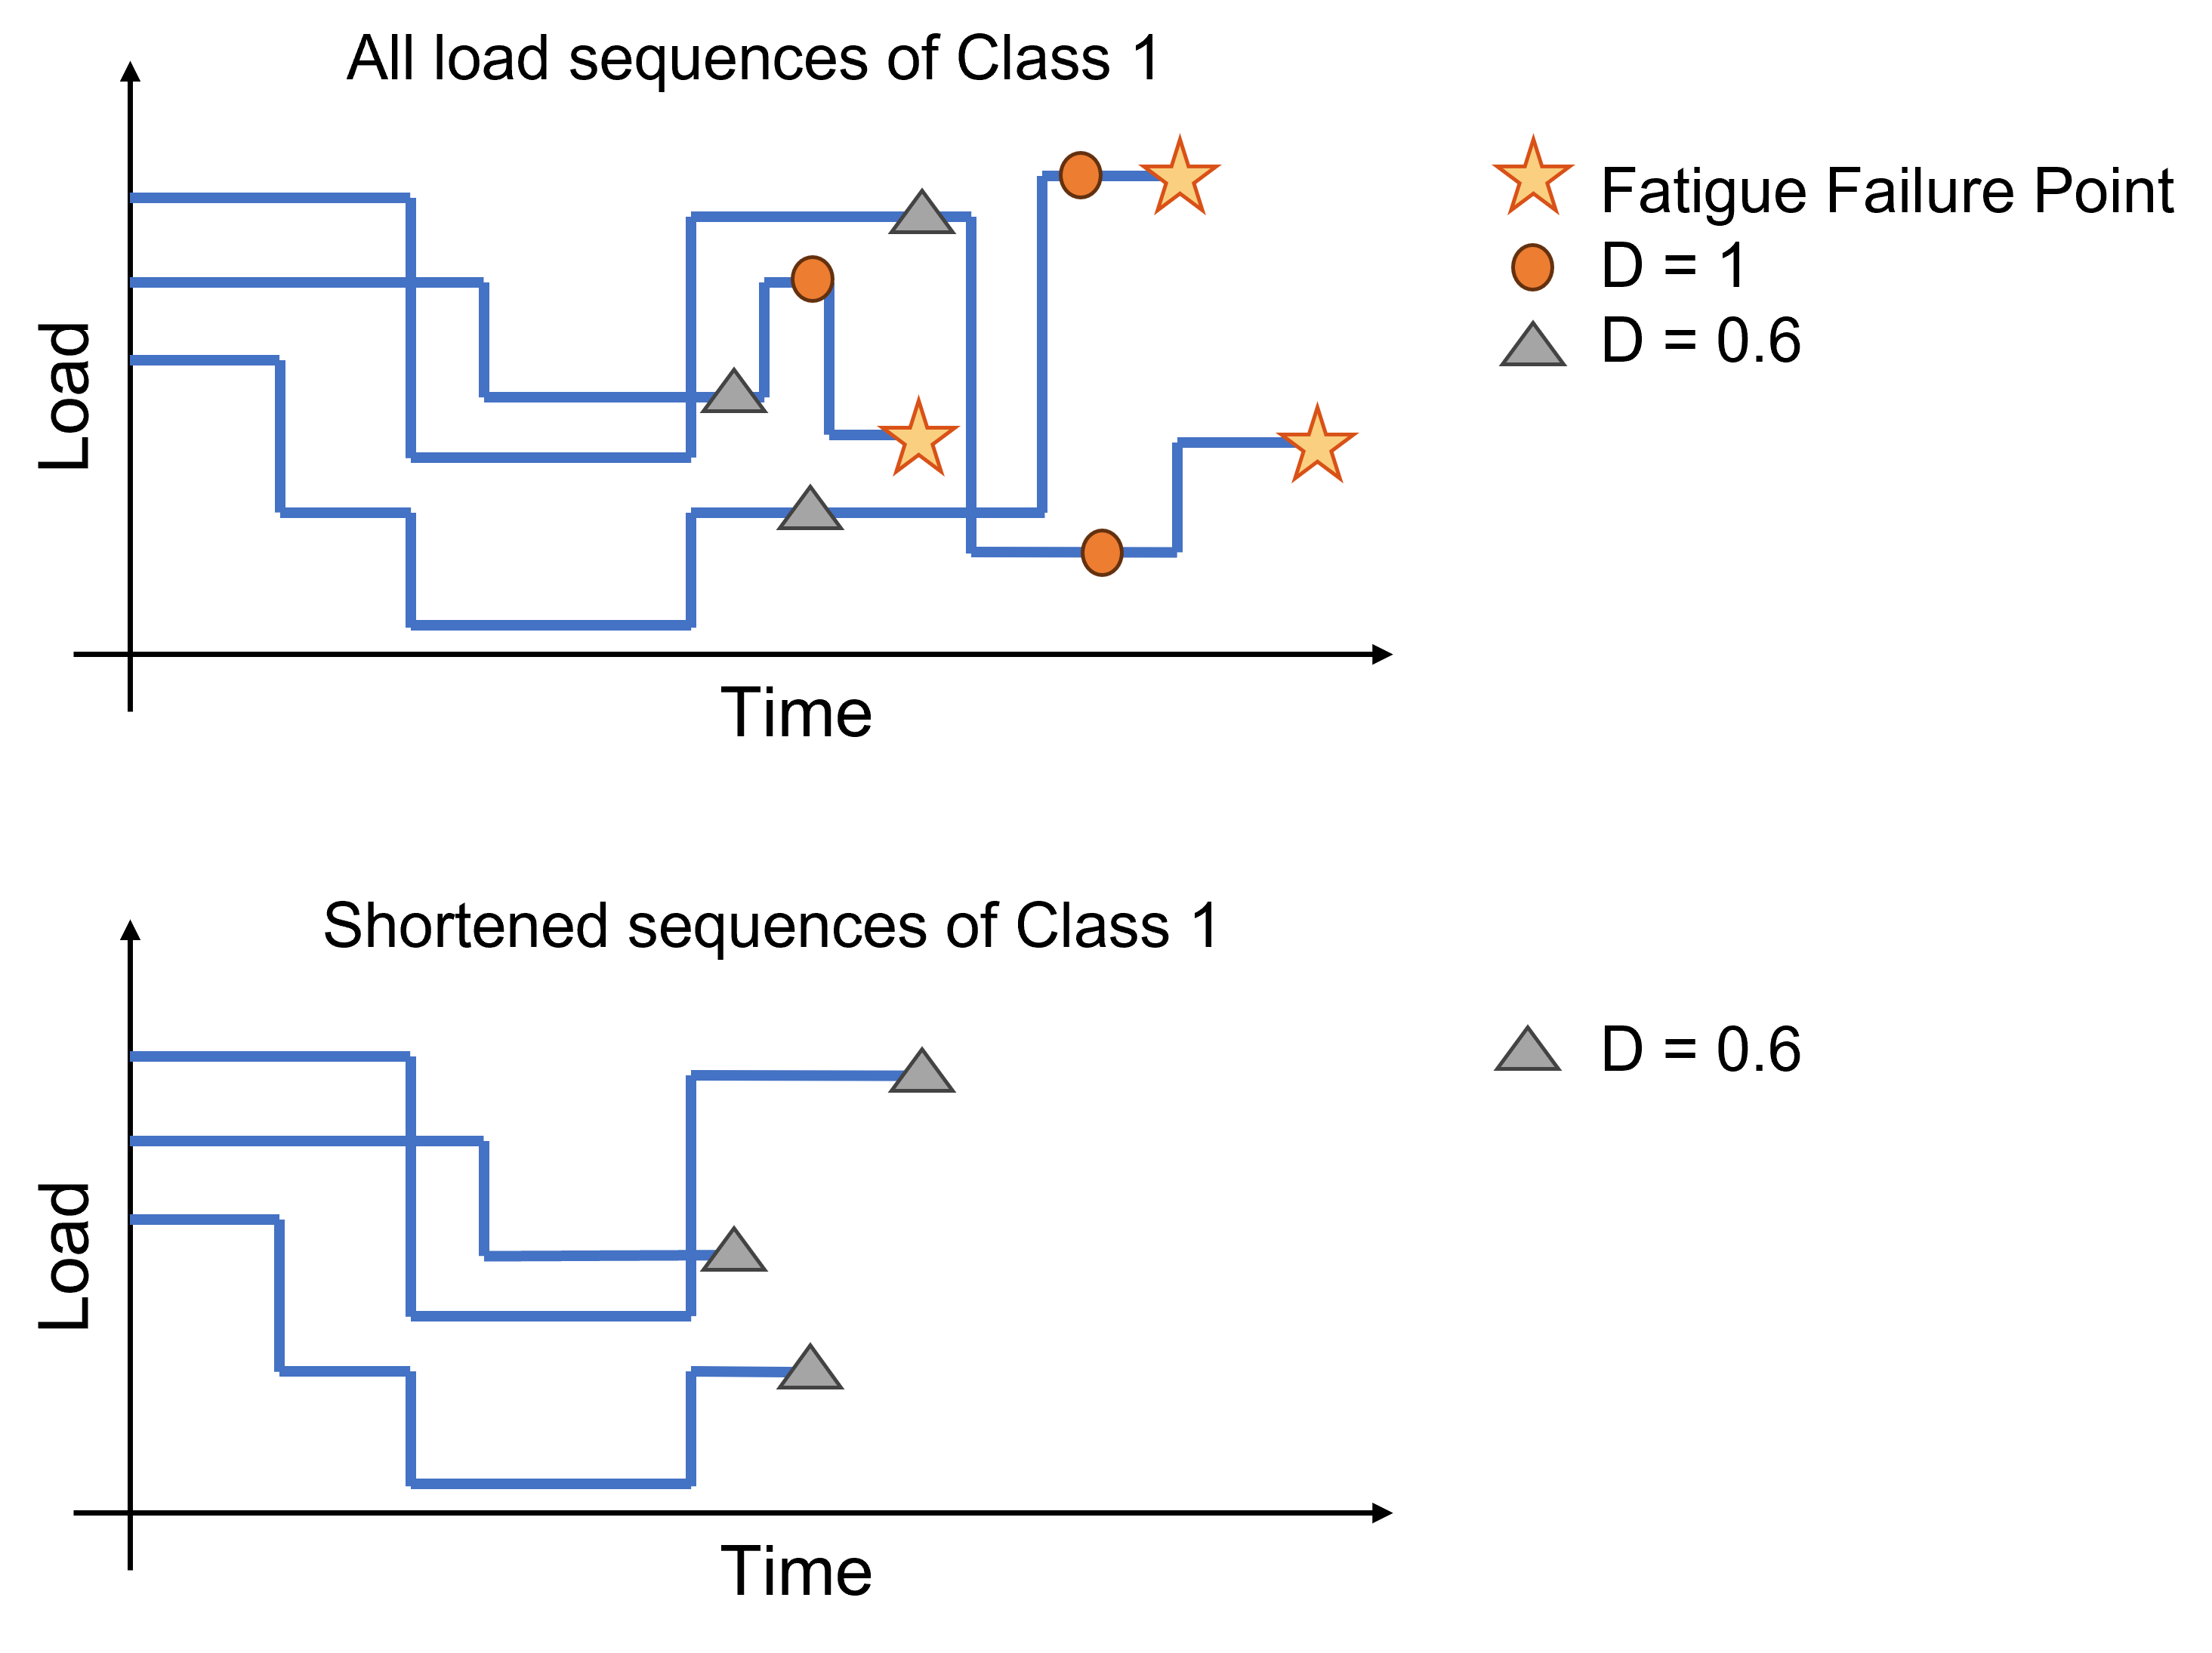
\includegraphics[width=0.8\linewidth]{IMGs/Shortened.png}
	\caption{Load sequence shortening}
	\label{fig:Shortened}
\end{figure}

\subsection{Problems in Classification of Sequences}
One of the problems in classifying sequences, is the difference in length of those sequences. The original recordings can have a different number of cycles which makes it difficult to use them as input-vectors. Most algorithms require a constant input-vector size for training and validation. This problem can be circumvented by pre-filling each augmented and reduced sequence with zeros to a uniform length or using a approach that can work with sequences of different sizes. 


The only problem remaining is the prediction of a unseen sequence that might be longer than any other sequence seen in training.
This problem can be solved by pre-pending more zeros to create a buffer for the ability to classify longer sequences than those present in the training data.


\newpage
\section{Regressor for SOH-Prediction}
The regressor is used as a linear extrapolation model that calculates the SOH of a gear. The SOH can be interpreted as a value for how soon the gear is expected to fail. For example, if the Miner rule calculates a damage sum D equal to 0.8, the classifier assigns a class label of 1 (not damaging load history), and the regressor calculates a SOH of 0.9, the gear is expected to be able to withstand higher loads but not for a very long time. In that case, it is expected that the damage sum D will accumulate past unity but will be limited in the number of cycles it can withstand. 

\subsection{Data-set for Regressor}\label{PrRe}
If an unfinished load sequence is classified into a class, for example class 1, the regressor will only be trained on the load sequences belonging to that class. Each augmented load sequence is iteratively selected and n different, randomly determined, points are chosen. These points are transferred to the label function of that sequence to determine the label (SOH) of that sequence-snipped from the beginning up to that point. The selected snippets are then saved and used as training data for the regressor.   
Figure \ref{fig:dataregressor} shows the process of creating data samples form one load sequence.

\begin{figure}[H]
	\centering
	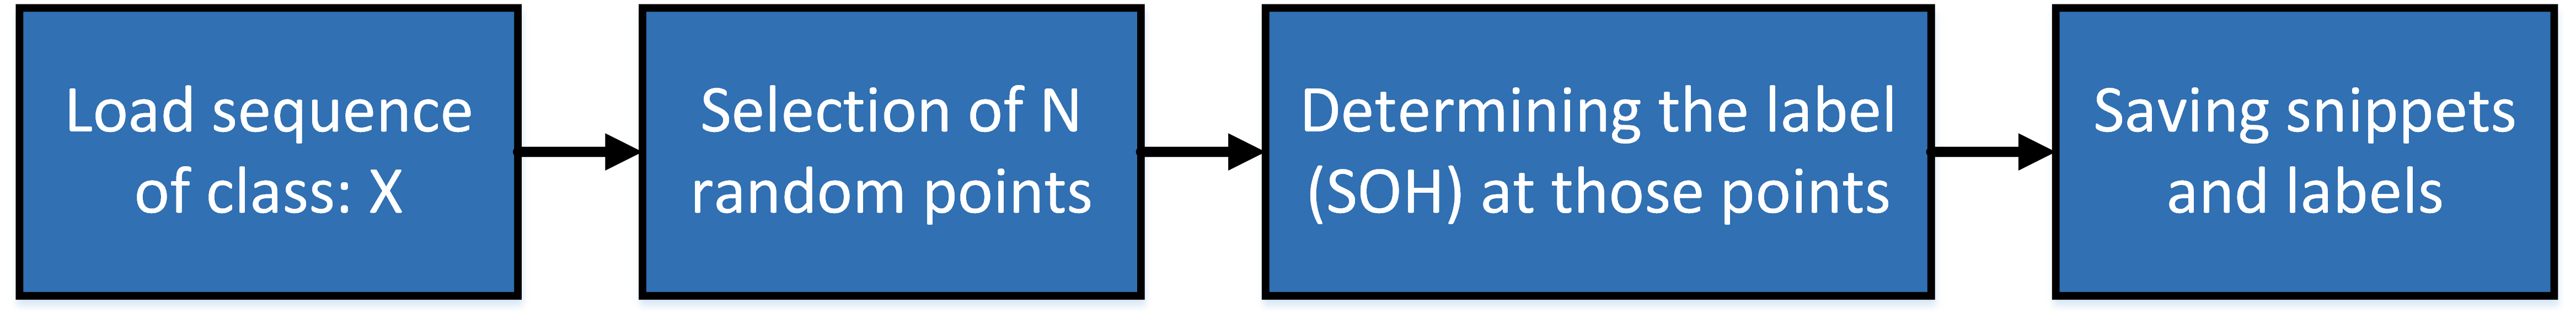
\includegraphics[width=0.85\linewidth]{IMGs/dataregressor.png}
	\caption{Data-set generation process for the regression data-set}
	\label{fig:dataregressor}
\end{figure}

Figure \ref{fig:4elems} gives a visual example on how three elements and the according labels are created form one load sequence. The number of created elements can be freely defined.

\begin{figure}[H]
	\centering
	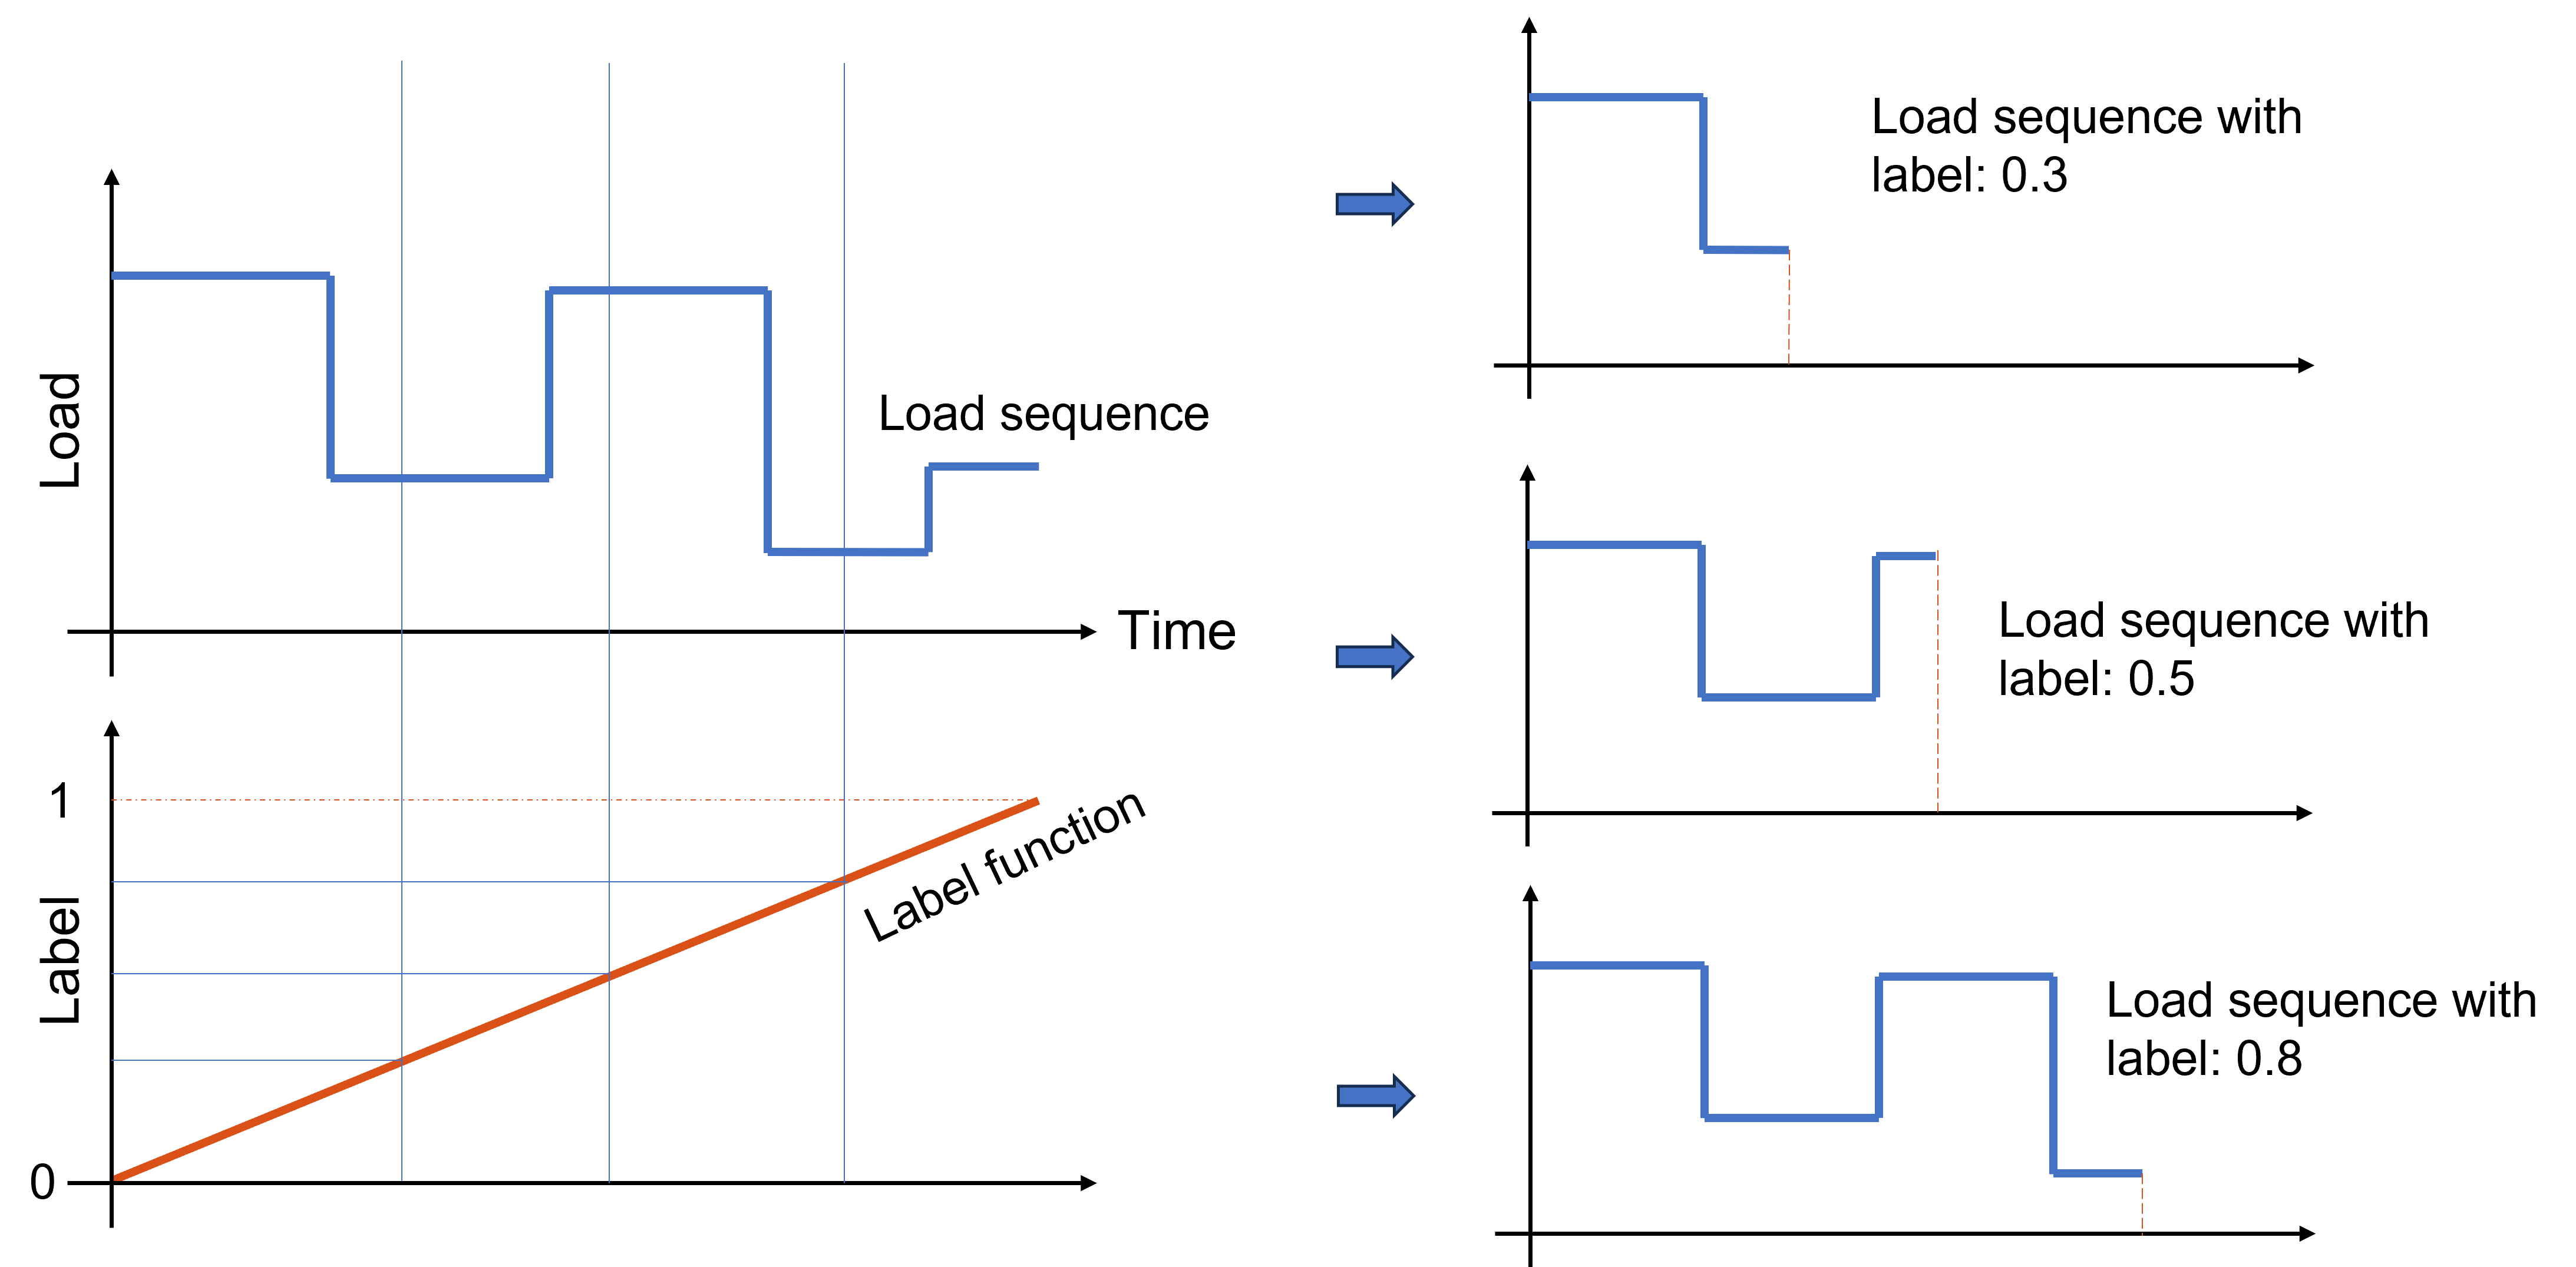
\includegraphics[width=0.95\linewidth]{IMGs/4elems.png}
	\caption{Creation of 3 elements with the help of the label function}
	\label{fig:4elems}
\end{figure}
\subsection{Training the Regressor}
The created training data-set has the same structure as the classification trainig-set. The sections are now of different lengths, not only because of the different number of cycles, but because of the different selected points. The regressor must either be able to accept input vectors of different sizes or each sequence needs to be pre-filled with zeros (zero-padding) to bring all elements to the same length.
\section{Summary of the Proposed Method}
The goal of the proposed method is to get a confidence value regarding the calculated damage sum D according to the Miner rule. It achieves that by first classifying a sequence into a category that represents the influence of the order of the loads. By doing so, it can be determined  if the Miner rule is giving a conservative or lenient estimate. The classification is based on a supervised learning algorithm that uses load sequences that failed before and after reaching a accumulated damage sum D equal to unity. The second step is a regressor that predicts a state-of-health, which is a value calculated by extrapolating the expected failure point in time based on the load sequences that have the same effect based on the order of loads. With these two values, the confidence in the calculated damage sum D can be evaluated.
Table \ref{cases} gives a overview on how to interpret the different combination of the two values. 

\begin{table}
	\begin{center}
		\begin{tabular}{|| r | l | l ||}
			\hline
			\rule{0pt}{2ex}Class & SOH & Effect\\
			\hline
			\hline
			\rule{0pt}{2ex}-1 (Very damaging)&  0,5 & will fail at D<1, but can withstand many cycles with low load\\\hline
			1 (less damaging)& 0,5 & will fail at D>1, and can withstand many cycles with high load\\\hline
			-1 (Very damaging)&  0.9 & Will fail very soon\\\hline
			1 (less damaging)& 0.9 & Will fail very soon but exceed D=1 if future load are high\\\hline
			\hline
		\end{tabular}
		\caption{Effect of the predicted class and SOH}
		\label{cases}
	\end{center}
	\vspace{-4mm}
\end{table}



% !TeX spellcheck = en_US 
\chapter{Validation}\label{Validation}
This chapter covers the implementation and results of the proposed method in chapter \ref{MET}.

\section{Implementation}
\subsection{General Information regarding the Implementation}
The method is implemented in Python 3.9.9 for its widespread availability of libraries for ML-algorithms.
The libraries from which the classifiers and regressors are taken are:\newline "scikit-learn"~\cite{SKlearn}, "TSlearn"~\cite{tslearn} and "xgboost"~\cite{XG}.
Multiple models from those libraries are tested and compared regarding their performance. %Runtime comparisons are not performed.
\subsection{Data Cleanup}
The first step is the cleanup of the data and its translation into a more flexible format. The recordings of the load sequences are provided in a text-file format that includes information such as displacements of the piston, cycle-time and cycle-count.
Figure \ref{fig:recordinglabel} shows all the labels of the recorded values in the txt-file and their interpretation. All information is disregarded except the net force at each cycle-peak. The net force is the absolute clamping force (lowest acting force) plus the recorded absolute peak (highest acting force). The order of loads is kept, and the absolute values are transformed into an array that is stored as a NumPy file (np-file). 14 load sequences are available, which are transformed into 14 np-files and stored in a new folder. The np-file format allows for faster read times and takes up less space on the hard drive than the original txt-files. The names are not important and are thus also replaced by a simple index.


\begin{figure}[H]
	\centering
	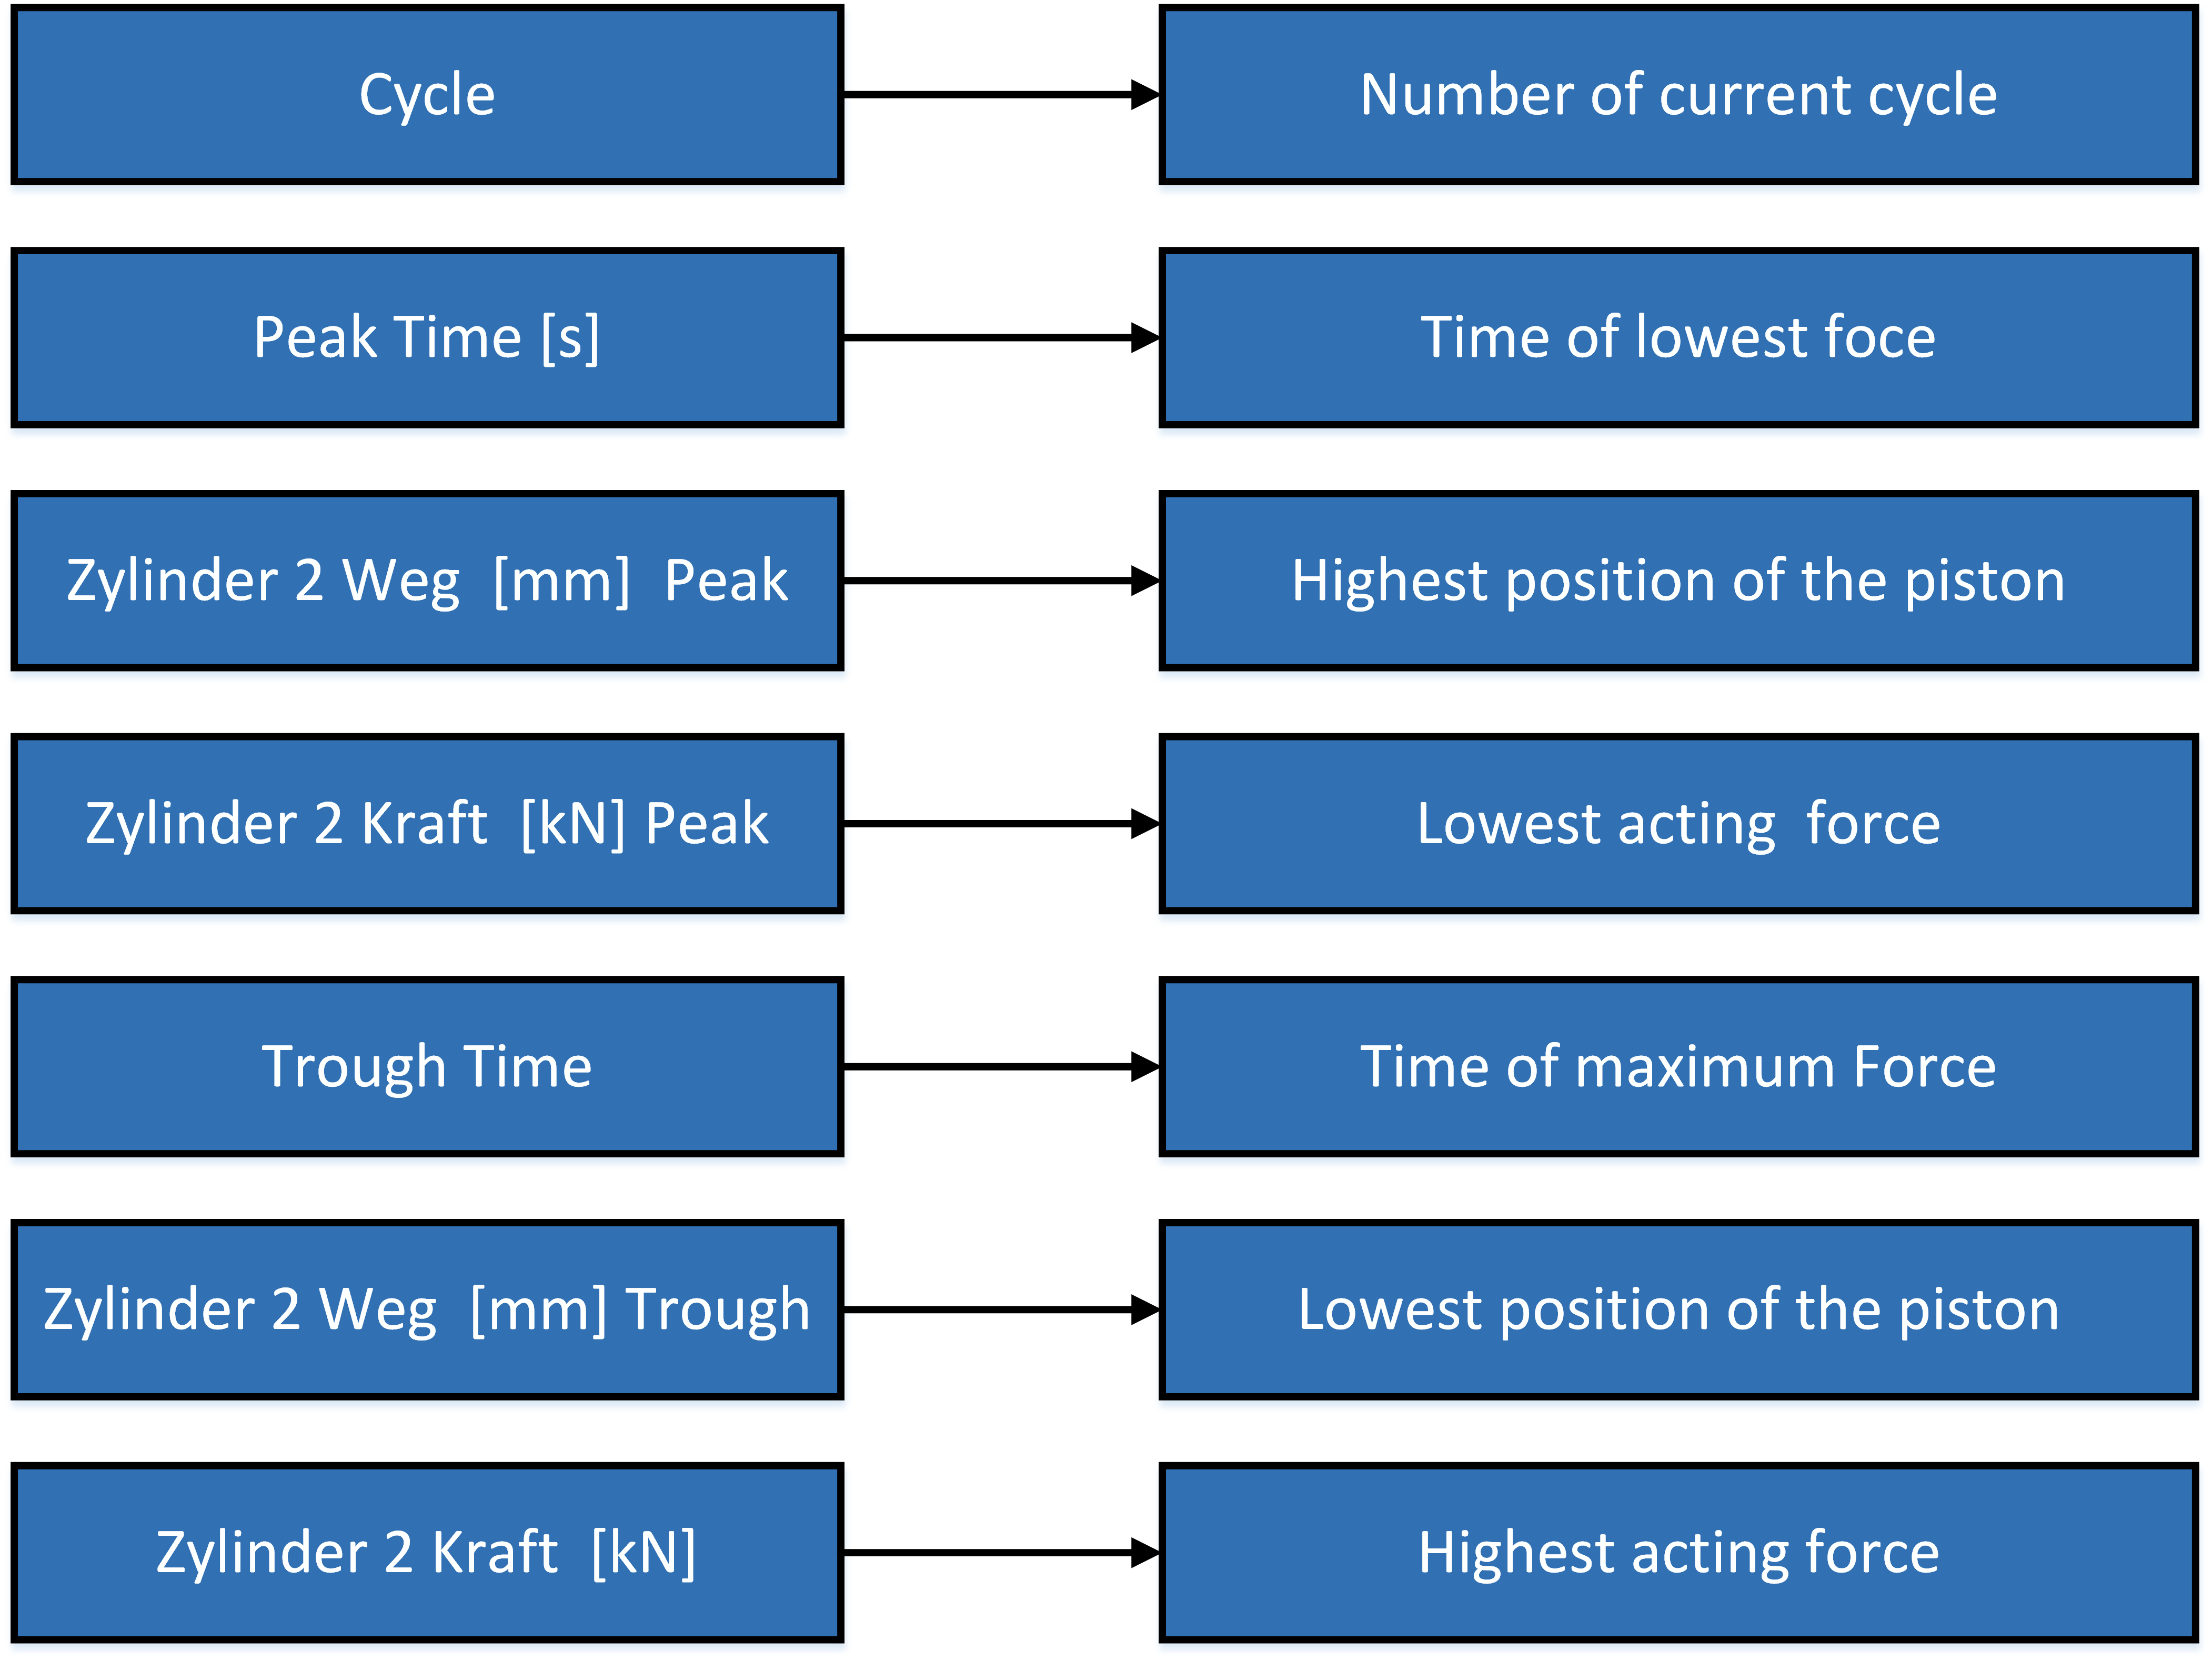
\includegraphics[width=0.75\linewidth]{IMGs/recordinglabel.png}
	\caption{Recorded parameters in STBF}
	\label{fig:recordinglabel}
\end{figure}

\subsection{Data Augmentation}
The data augmentation process starts with calculating the damage sum D with the help of the Basquin equation (see equation \ref{BQ}) and the Miner rule (see equation \ref{acc}).
The parameters for the Basquin equation were provided and shown in table \ref{paramBQ}.
Only forces higher than the endurance limit are selected when calculating the accumulated damage. The calculated damage sum D according to the Miner rule for each available file are shown in table \ref{DamageSUMS}


\begin{table}
	\begin{center}
		\begin{tabular}{|| r | l ||}
			\hline
			\rule{0pt}{2ex}Load Sequence Nr. & Damage sum D\\
			\hline
			\hline
			\rule{0pt}{2ex}0 & 2.16\\ \hline
			1 & 1.18\\	\hline
			2 & 1.29 \\ \hline
			3 & 0.92\\ \hline
			4 & 3.4 \\ \hline
			5 & 1.18 \\ \hline
			6 & 1.4 \\ \hline
			7 & 1.01 \\ \hline
			8 & 1.06 \\ \hline
			9 & 0.75 \\ \hline
			10 & 0.68 \\ \hline
			11 & 1.22\\ \hline
			12 & 0.73 \\ \hline
			13 & 1.1 \\ \hline

		\end{tabular}
		\caption{Damage sum D at failure of available load sequences}
		\label{DamageSUMS}
	\end{center}
	\vspace{-4mm}
\end{table}


\begin{table}
	\begin{center}
		\begin{tabular}{|| l | l ||}
			\hline
			\rule{0pt}{2ex}Parameter D & Value\\
			\hline
			\hline
			\rule{0pt}{2ex}Slope of the S-N fatigue strength curve = k & 6.33048\\ \hline
			Reference value of fatigue strength = C & 11670367740000000\\	\hline
			Value of the load at one cycle = L & values from array \\ \hline
			Endurance limit & 56.618 kN \\ \hline
		\end{tabular}
		\caption{Parameters of the Basquin-equation and Endurance Limit}
		\label{paramBQ}
	\end{center}
	\vspace{-4mm}
\end{table}

The first step in DA is the addition of random noise. A np-file is loaded and the damage~sum~D is calculated. That value serves as a reference to compare if the augmentation significantly changes the damage sum D.
The random noise is in the form of a vector that has the same length as the loaded load sequence.
The individual noise values follow a Gaussian distribution with a mean of 0 and a standard deviation of 0.2. 
The values of the noise vector are also in kN and thus can be simply added.
Figure \ref{fig:V5} shows a load sequence in its unedited form without the addition of noise. Figure \ref{fig:V5_noise} shows the same load sequence with the additional noise vector. As can be seen, the damage sum D is not changed enough to be noticeable when rounding to two decimal places, even though there is a clearly visible difference in the load sequences.

\begin{figure}[H]
	\centering
	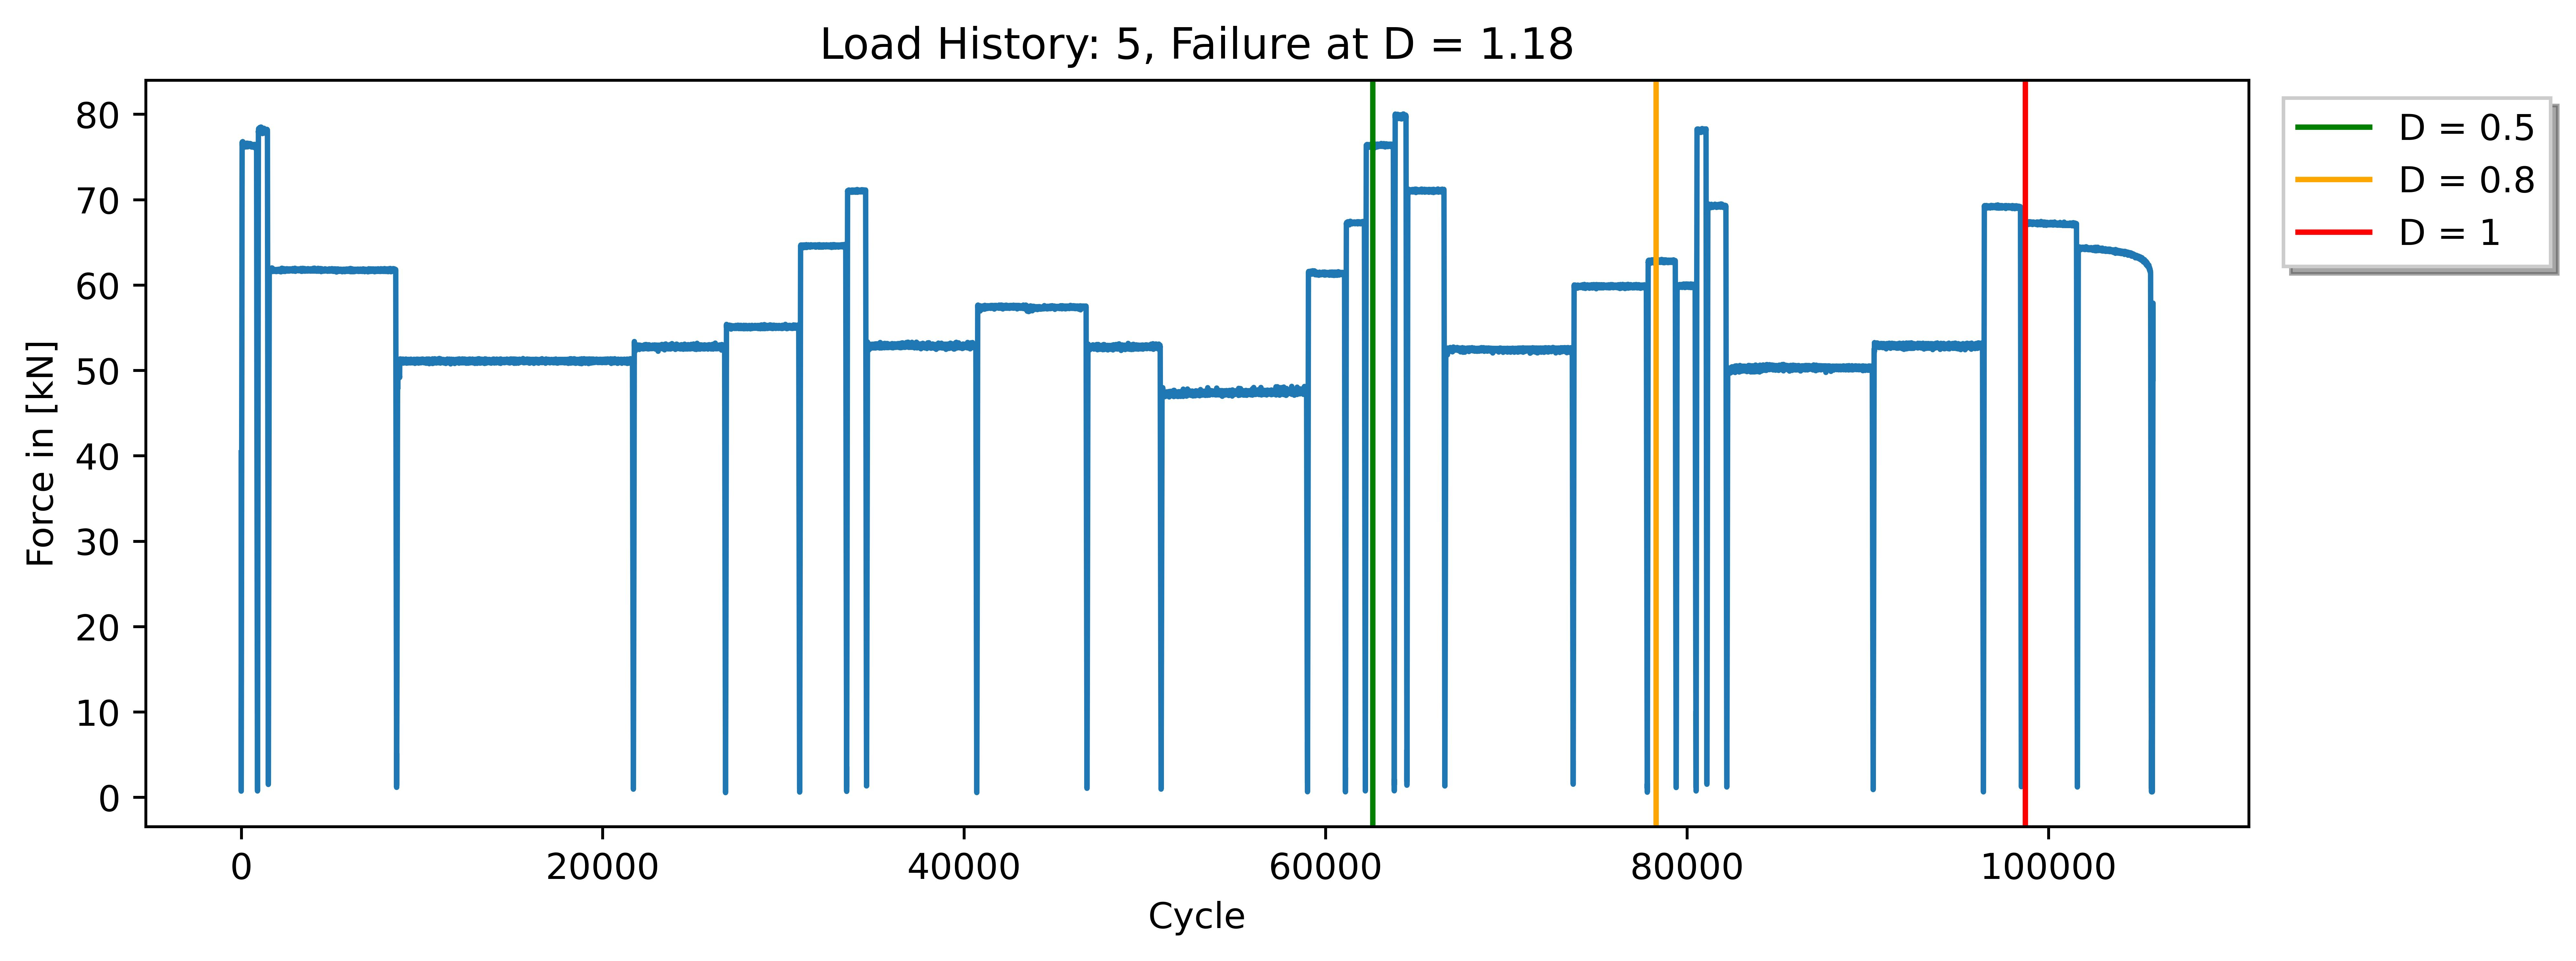
\includegraphics[width=1\linewidth]{IMGs/Verlauf_5.jpg}
	\caption{Load sequence without DA}
	\label{fig:V5}
\end{figure}

\begin{figure}[H]
	\centering
	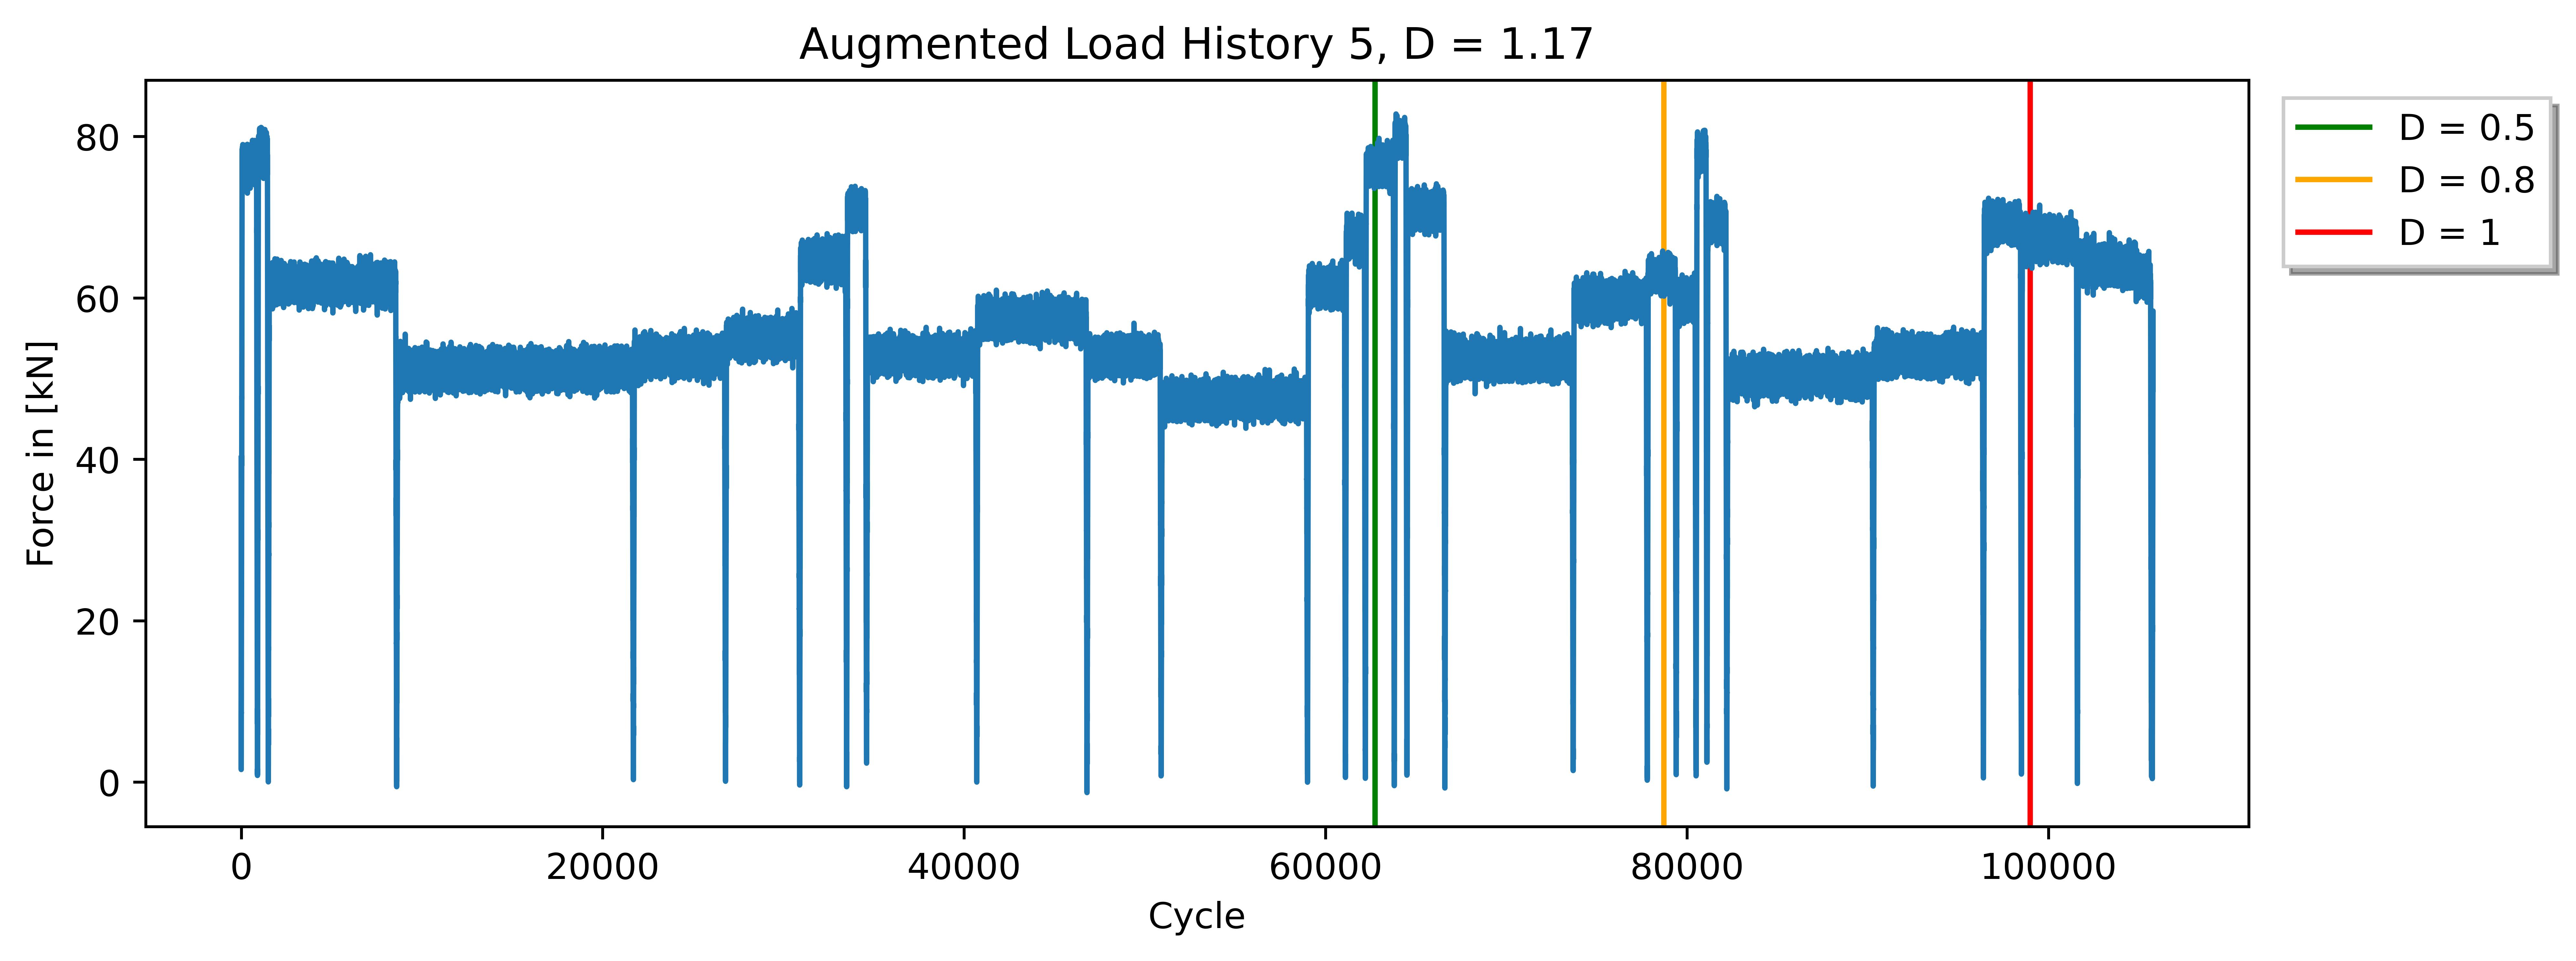
\includegraphics[width=1\linewidth]{IMGs/Verlauf_5_noise.jpg}
	\caption{Load sequence with additional noise}
	\label{fig:V5_noise}
\end{figure}

The second performed step is a global shift of the whole loading sequence up or down by up to 500 N. This is done by sampling a uniform distribution between -1 and 1 and multiplying by 0.5. This constant is added to every array element. Figure \ref{fig:V5_shift} shows the shifted load sequence with the previously added noise. In this case, the damage sum D is altered either in the negative or positive direction. Again, no significant changes occurred regarding damage sum D.

\begin{figure}[H]
	\centering
	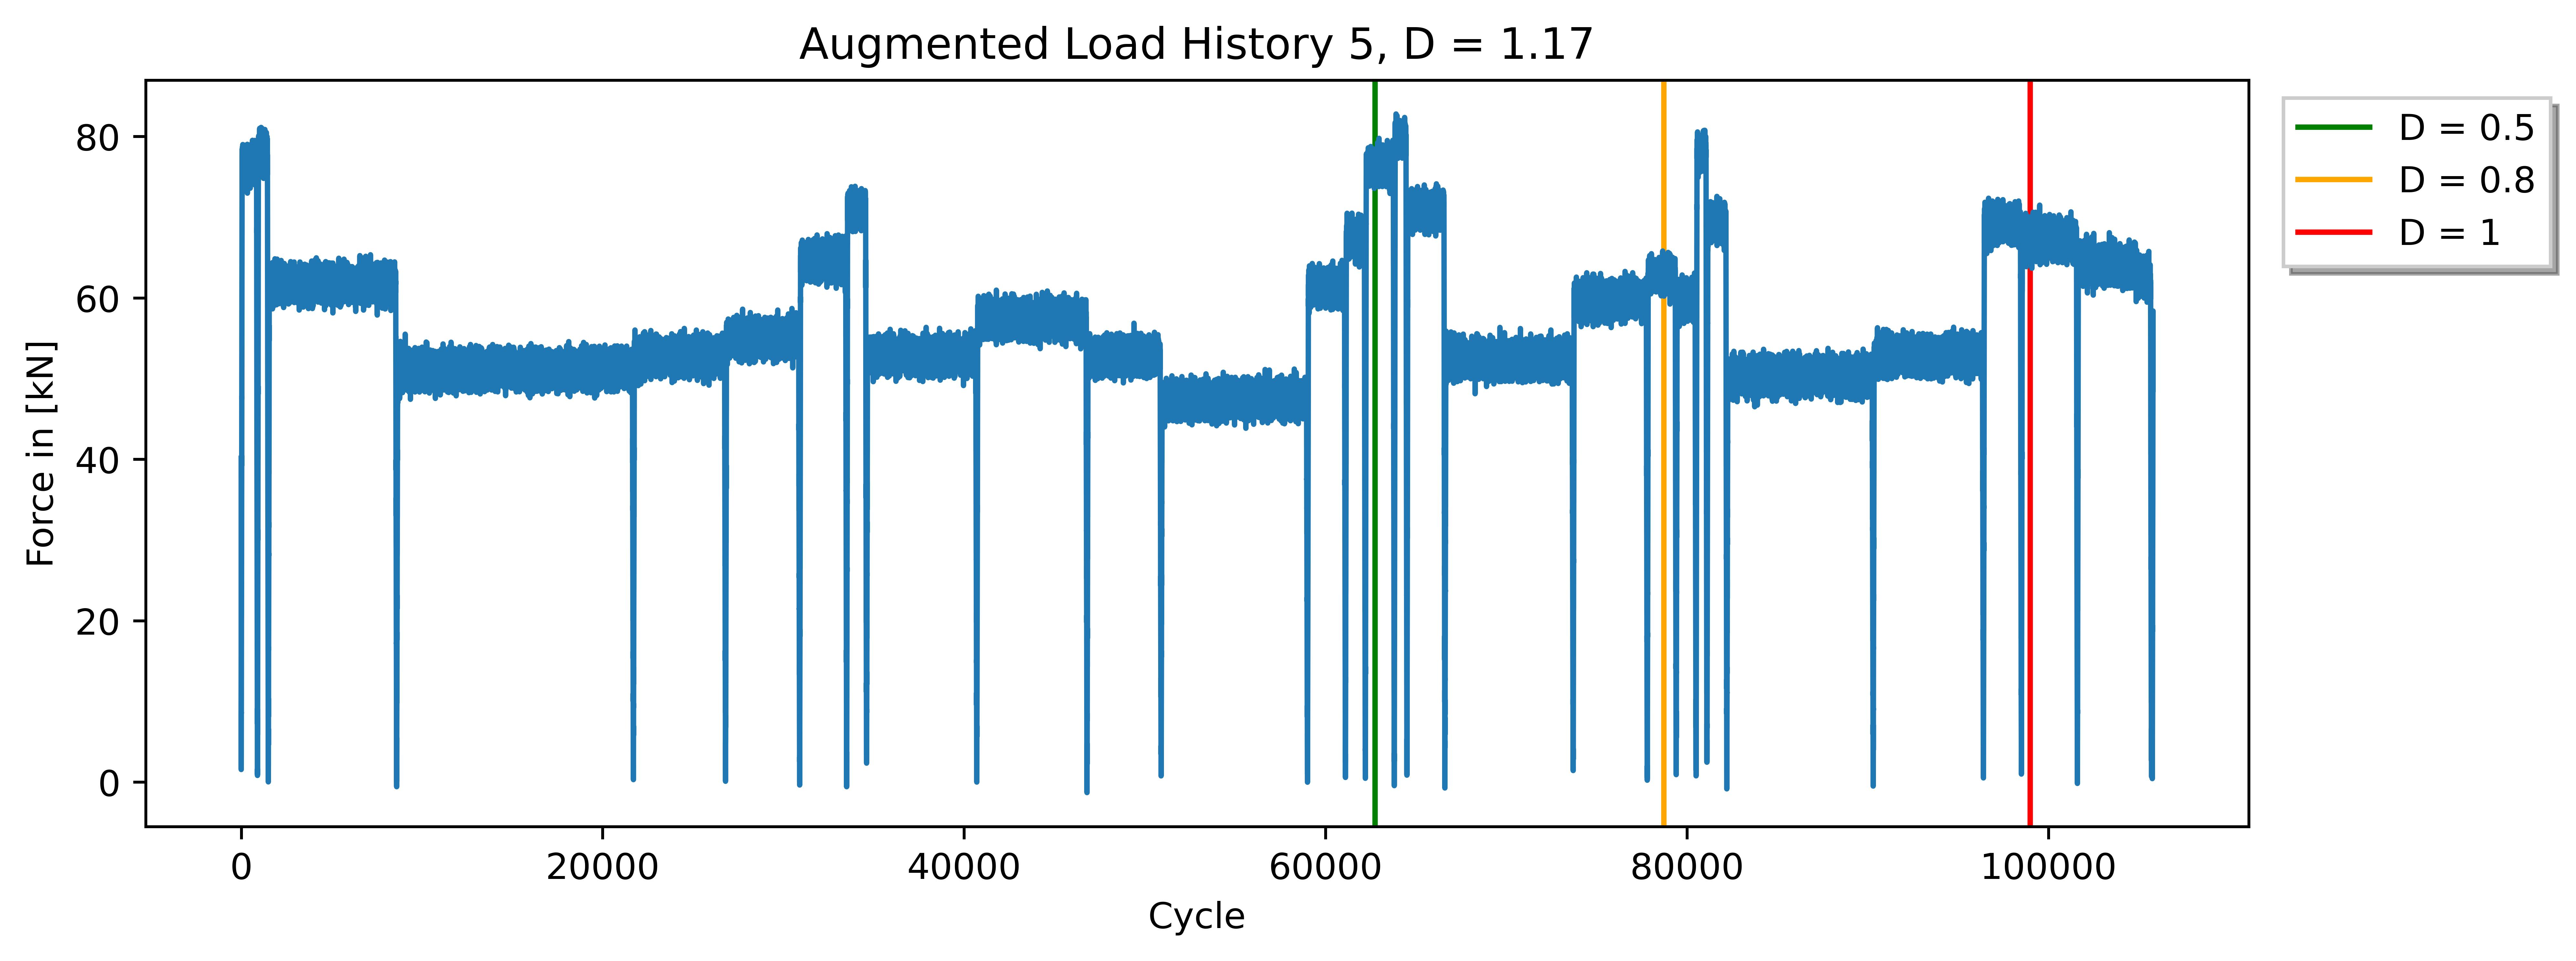
\includegraphics[width=1\linewidth]{IMGs/Verlauf_5_noise.jpg}
	\caption{Load sequence with noise and shift}
	\label{fig:V5_shift}
\end{figure}

The third step is a section-wise random shift. A random section of the array with a length of 1 \% of the total length is selected. This section is multiplied by a random factor taken from a uniform distribution between 0.5 and 1.5. So the force in that section is either increased or decreased by up to 50 \%. This step is performed three times on one load sequence. This step effectively changes the values of 3 \% of the sequence. 

In this step, the damage sum D can change significantly. The most significant changes occur when the selected areas are overlapping and scaled in the same direction. In a worst-case scenario, the selected section includes a proportionally high load and is amplified it by a factor of up to~3.375~(1.5\(^3\)). This scenario is highly unlikely and in the case of a significant alteration of the damage sum D the augmented load sequence is discarded as explained previously in figure~\ref{fig:DAUG}.
 
Figure \ref{fig:Verlauf_5_shift_partial} shows how the load sequence is changed by applying that DA step. Notice the down-shifted area around the 92,000\(^{th}\) cycle.


\begin{figure}[H]
	\centering
	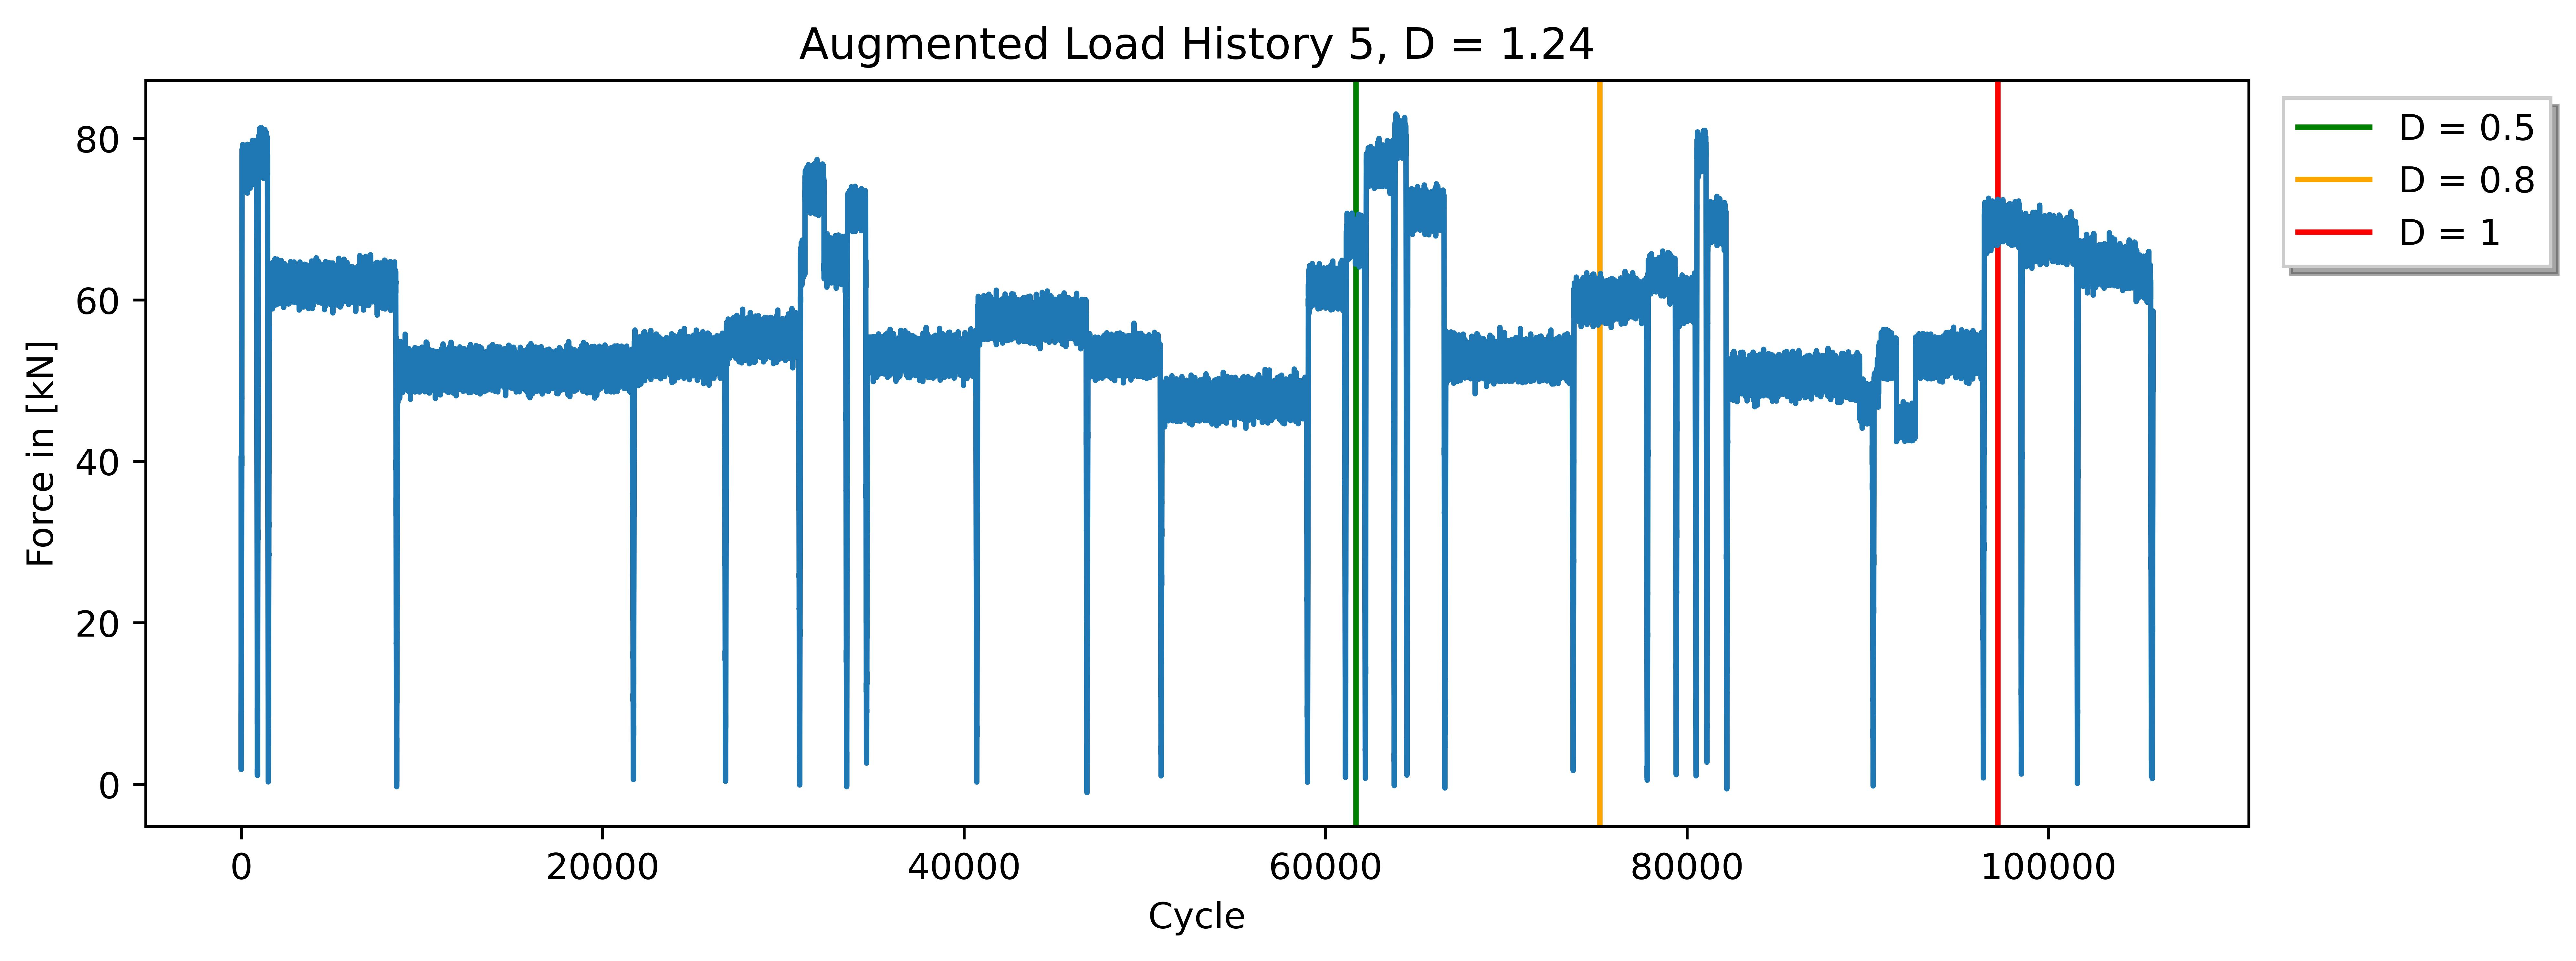
\includegraphics[width=1\linewidth]{IMGs/Verlauf_5_shift_partial.jpg}
	\caption{Load sequence with partial shift}
	\label{fig:Verlauf_5_shift_partial}
\end{figure}
\newpage
The fourth step is a partial cutout, where a random section of length of 1 \% of the total length is cut out of the sequence. In this step, the damage sum D is always decreased. Figure \ref{fig:Verlauf_5_cutout} shows how the loading sequence is transformed with partial cutouts.

\begin{figure}[H]
	\centering
	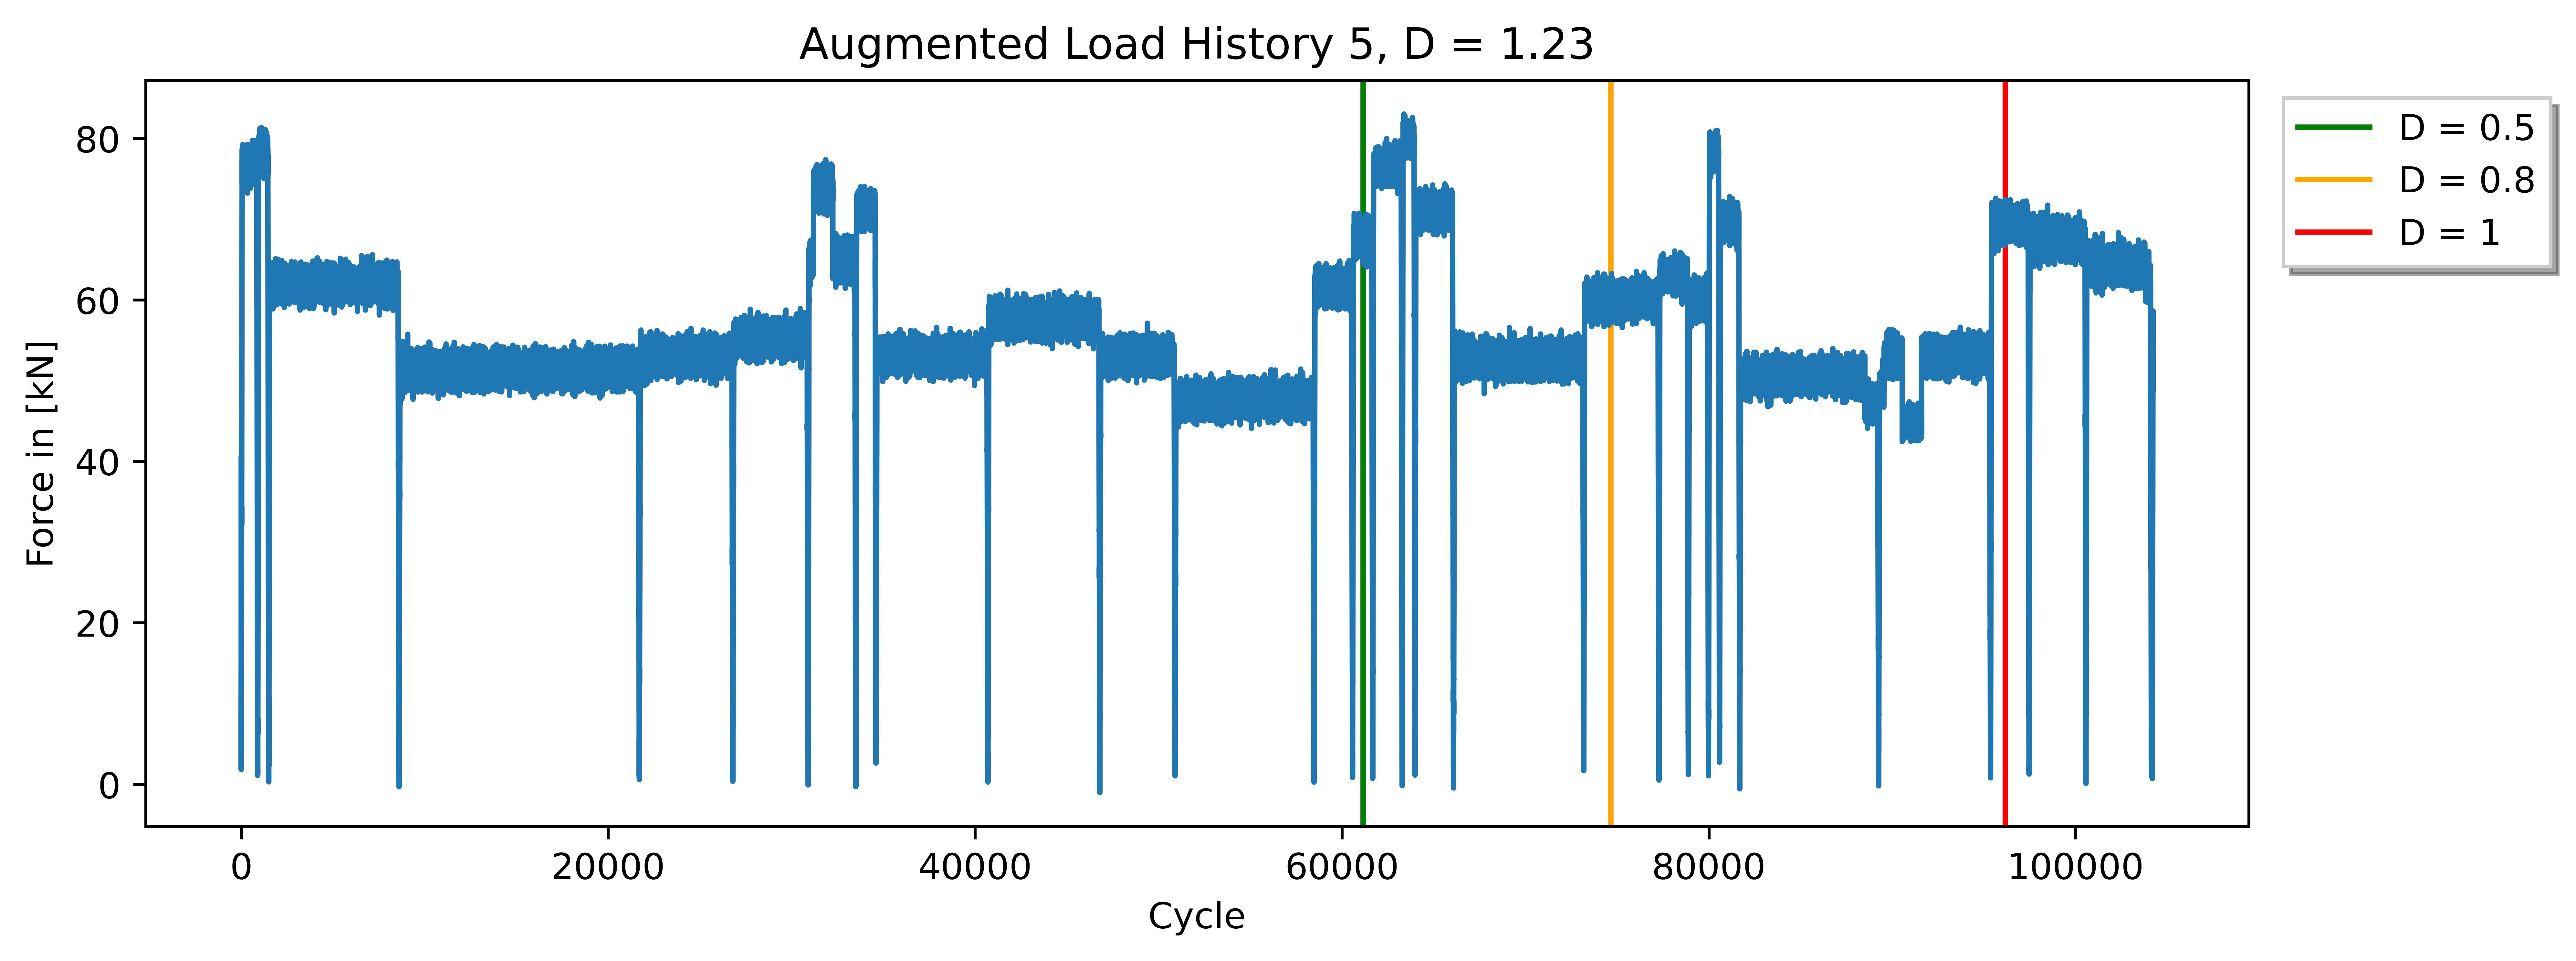
\includegraphics[width=1\linewidth]{IMGs/Verlauf_5_coutout.jpg}
	\caption{Load sequence with partial cutouts}
	\label{fig:Verlauf_5_cutout}
\end{figure}

The next step is the addition of a vector whose values are either going from positive to negative or from negative to positive over its length. It is essentially weighing the values of the load sequence over its length. By adding that vector to the load sequence, some values are increased while others are decreased. 

At first, a random variable decides if the sequence is tilted up (from negative to positive) or down (going from positive to negative). In the case of an upward shift, the start values of that vector are random variables selected from a uniform distribution in the range [-0.2, 0]. The last value is selected from a uniform distribution in the range [0, 0.2]. In the case of a downward shift, the ranges are switched.
The values between are interpolated accordingly with a constant step size.

Figure \ref{fig:Verlauf_5_tilt} shows all the previously mentioned DA-steps combined.

\begin{figure}[H]
	\centering
	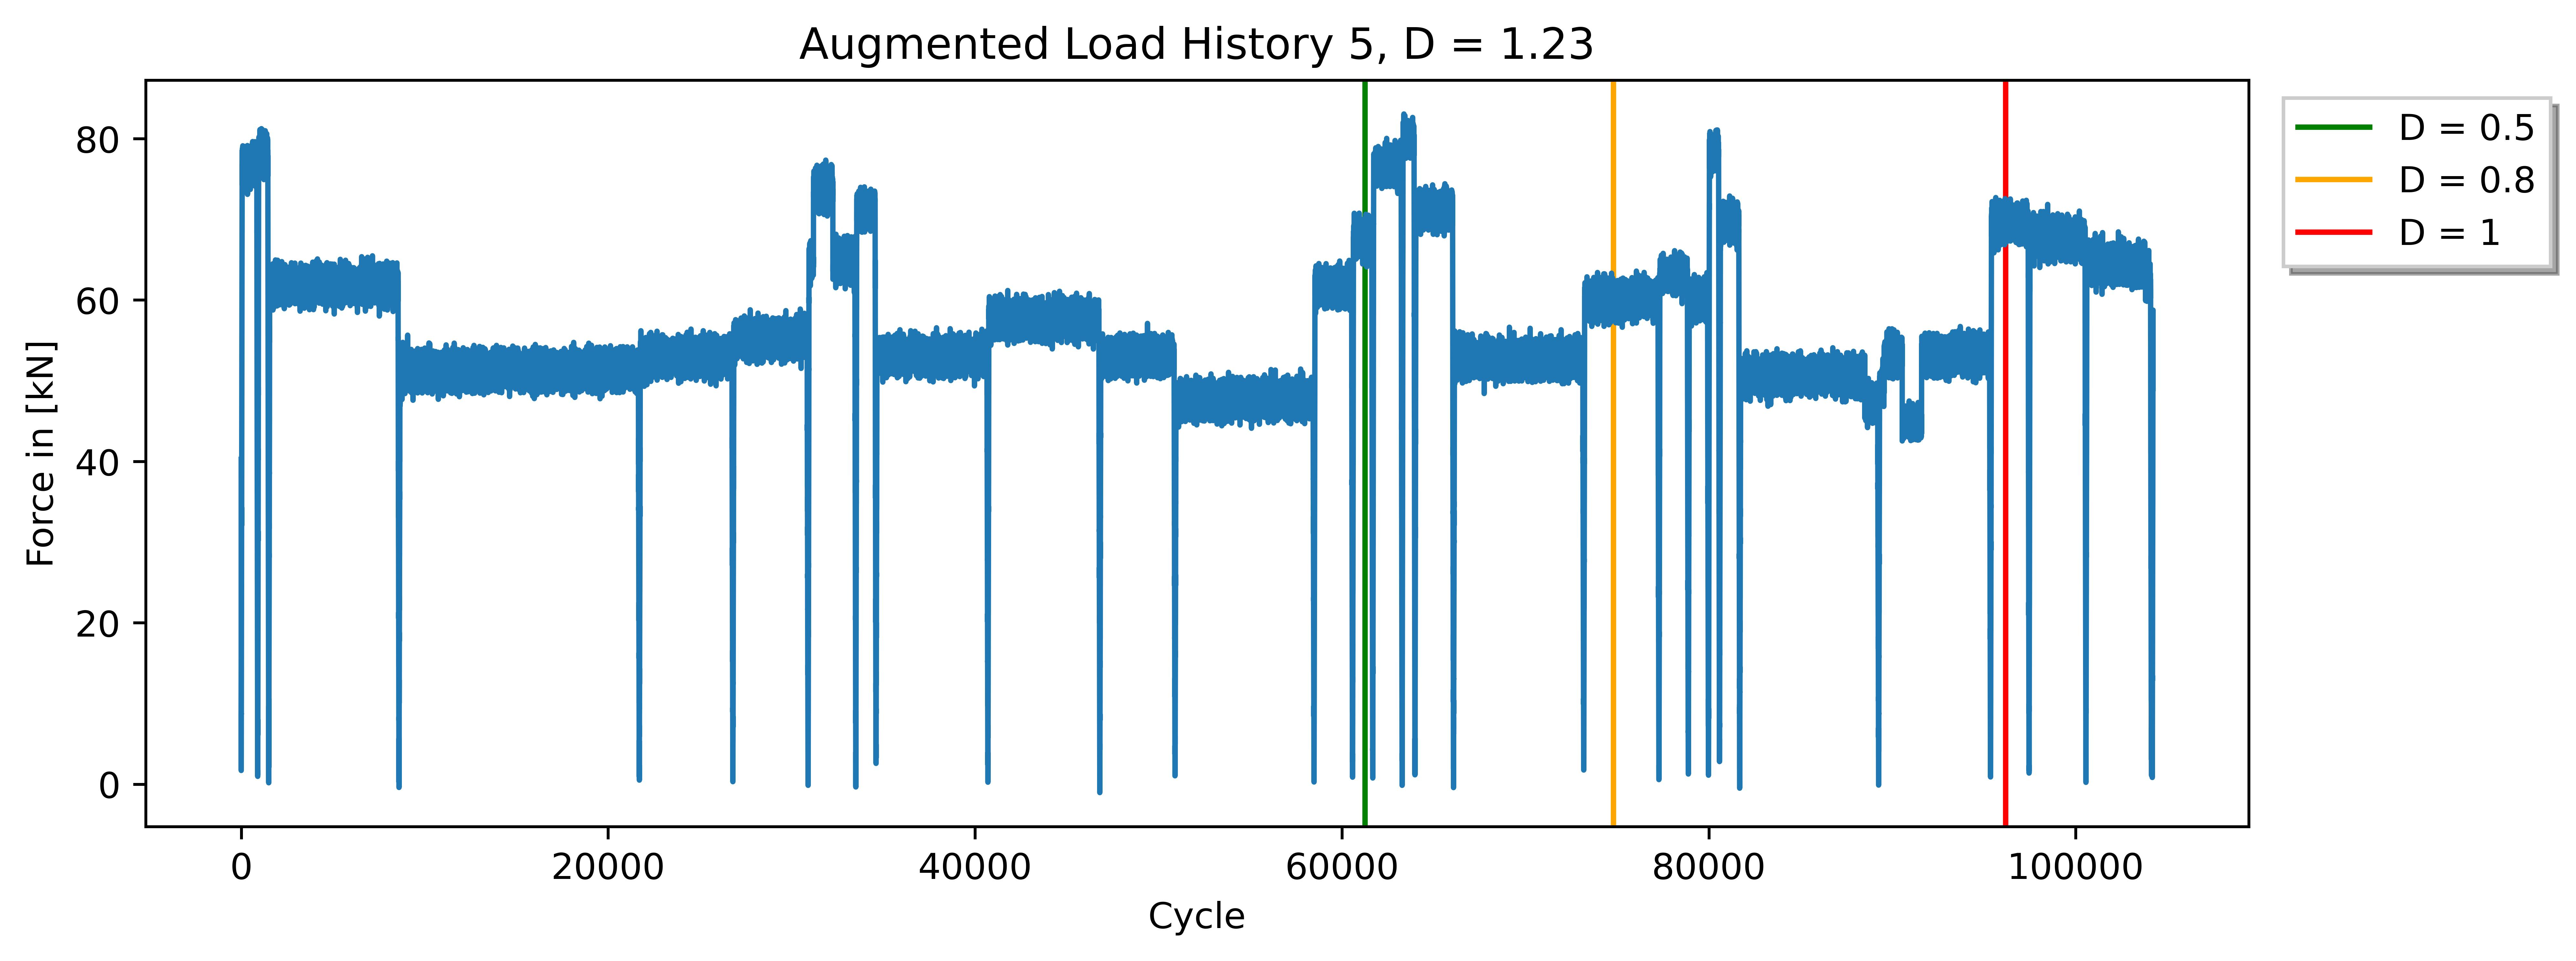
\includegraphics[width=1\linewidth]{IMGs/Verlauf_5_tilt.jpg}
	\caption{Load sequence with tilt}
	\label{fig:Verlauf_5_tilt}
\end{figure}

When comparing the original and the augmented load sequence, the visual difference is low. This is due to the fact that damage sum D must not change more than 10 \% of its original value. Only load sequences that fulfill this criteria are accepted into the training datasets.
To filter out all sequences that are off by 10 \% the original damage sum D and damage sum D after augmentation are compared.
If the ratio falls within [0.9, 1.1] the sequence is accepted and the final step is applied.


The last step is dimensionality reduction, as described in chapter \ref{prep_class}. In this case, every 300\(^{th}\) point in that sequence is kept. This step is effectively reducing the length of the sequence by a factor of 300. For the last comparison of the damage sum D, the denominator in the Miner rule must be multiplied by the step size. Again only if the ration falls within [0.9, 1.1], the sequence is accepted into the data-set. 

Figure \ref{fig:Verlauf_5_reduced} shows the load sequence in its reduced form. Notice that the characteristics of the original load sequence are still present.
 
\begin{figure}[H]
	\centering
	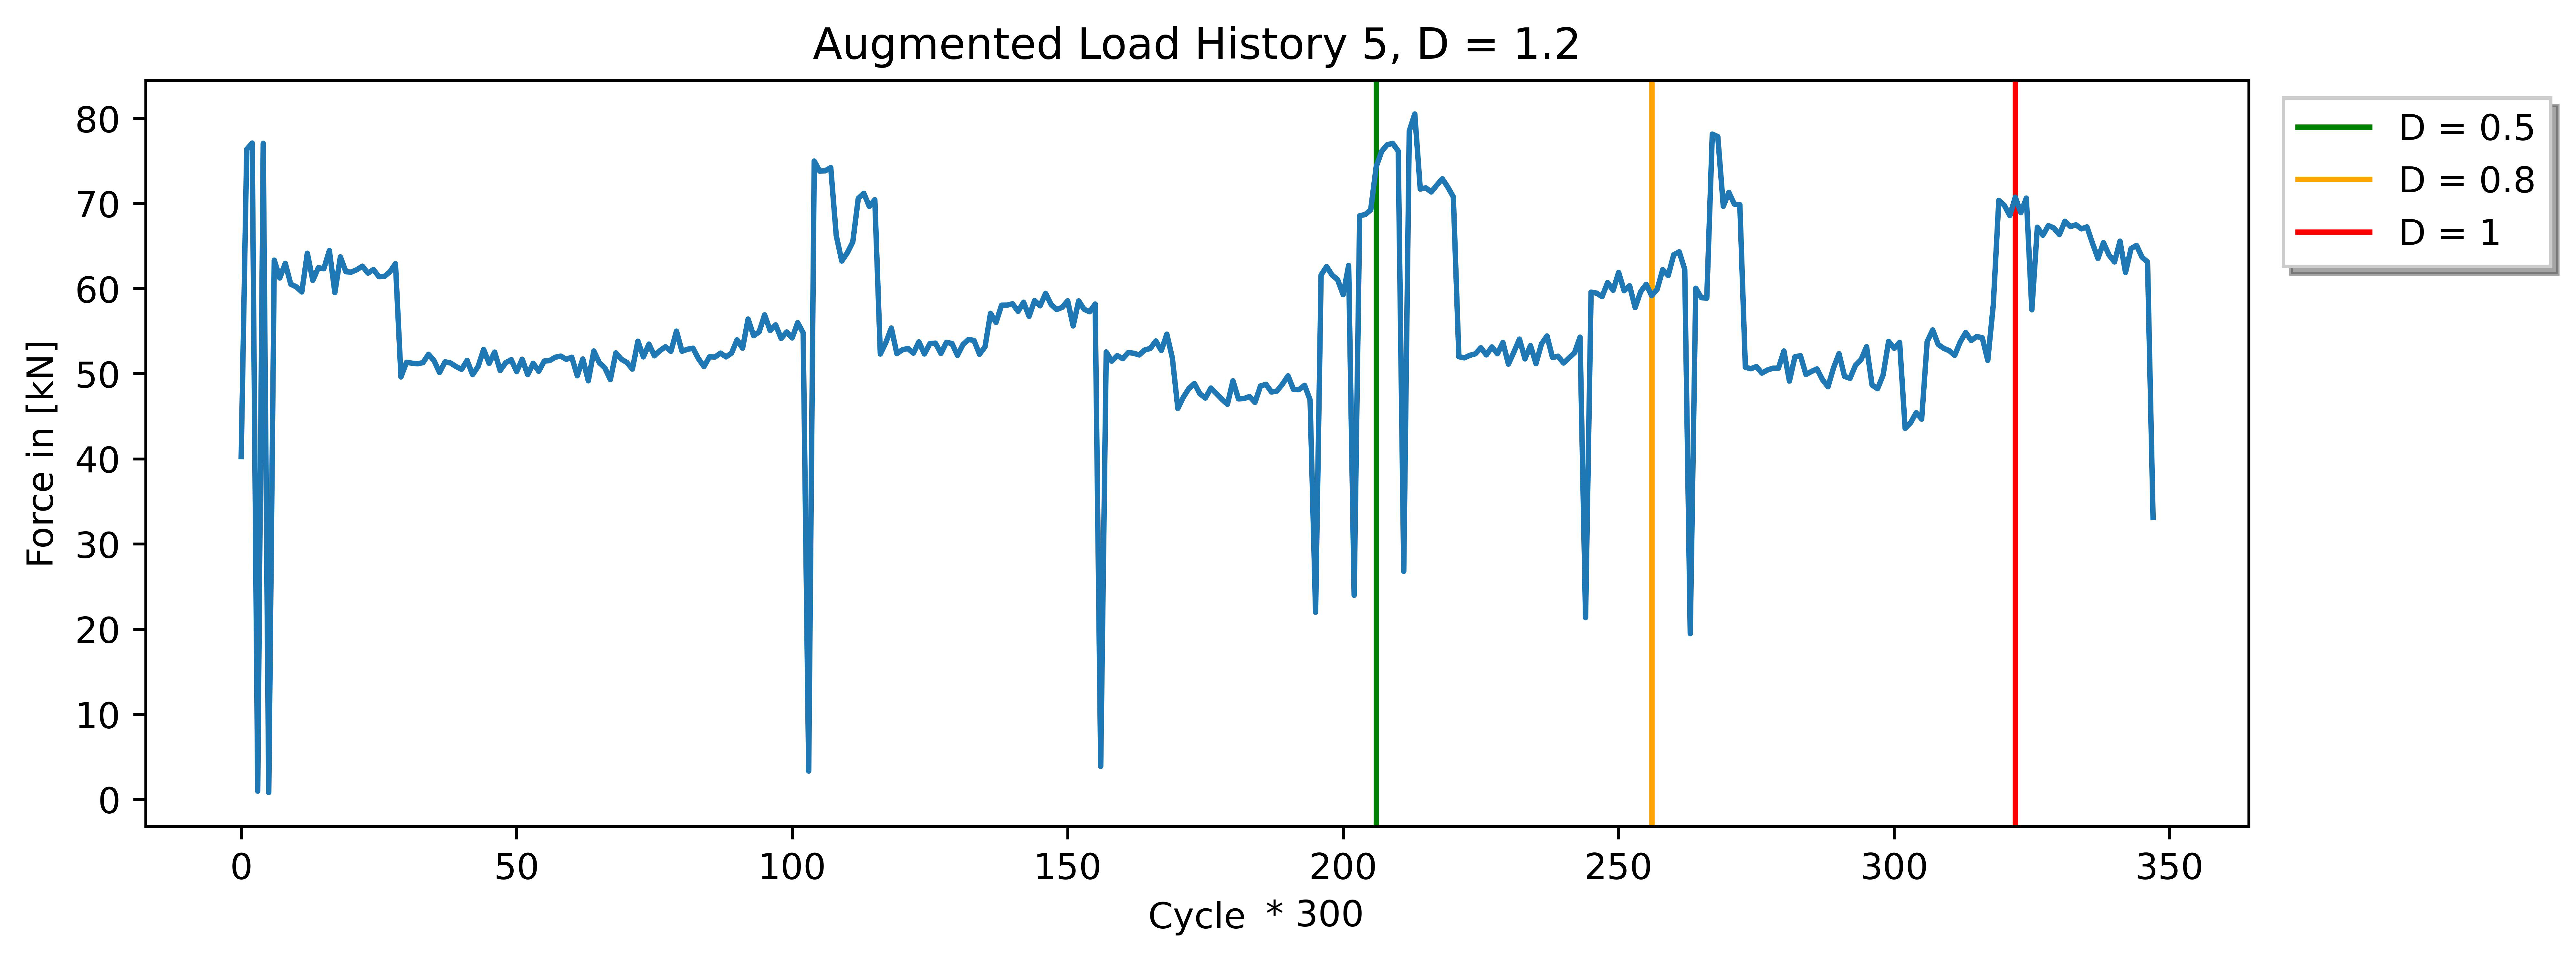
\includegraphics[width=1\linewidth]{IMGs/Verlauf_5_reduced.png}
	\caption{Load sequence after dimensionality reduction}
	\label{fig:Verlauf_5_reduced}
\end{figure}

Each load sequence is augmented with the described procedure 25 times. In the end, 25 individual instances can be present in the datasets if none of the augmented ones are filtered out. 
The accepted load sequences are saved as a np-array in a new separate folder. The name of the np-file follows the following pattern: [class\_idx.np]. "class" is the class to which the loading sequence belongs to, according to table \ref{DamageClass} and "idx" is a counting index that is increasing from 0 to n to keep track of the number of data samples.

Figure \ref{fig:3in1} shows only three out of those 25 augmented sequences in one plot to highlight the differences in each sequence.
Notice how the points of damage sum D of 0.5, 0.8 and 1 vary in their positions, but the characteristics of the original load sequence are kept.

\begin{figure}[H]
	\centering
	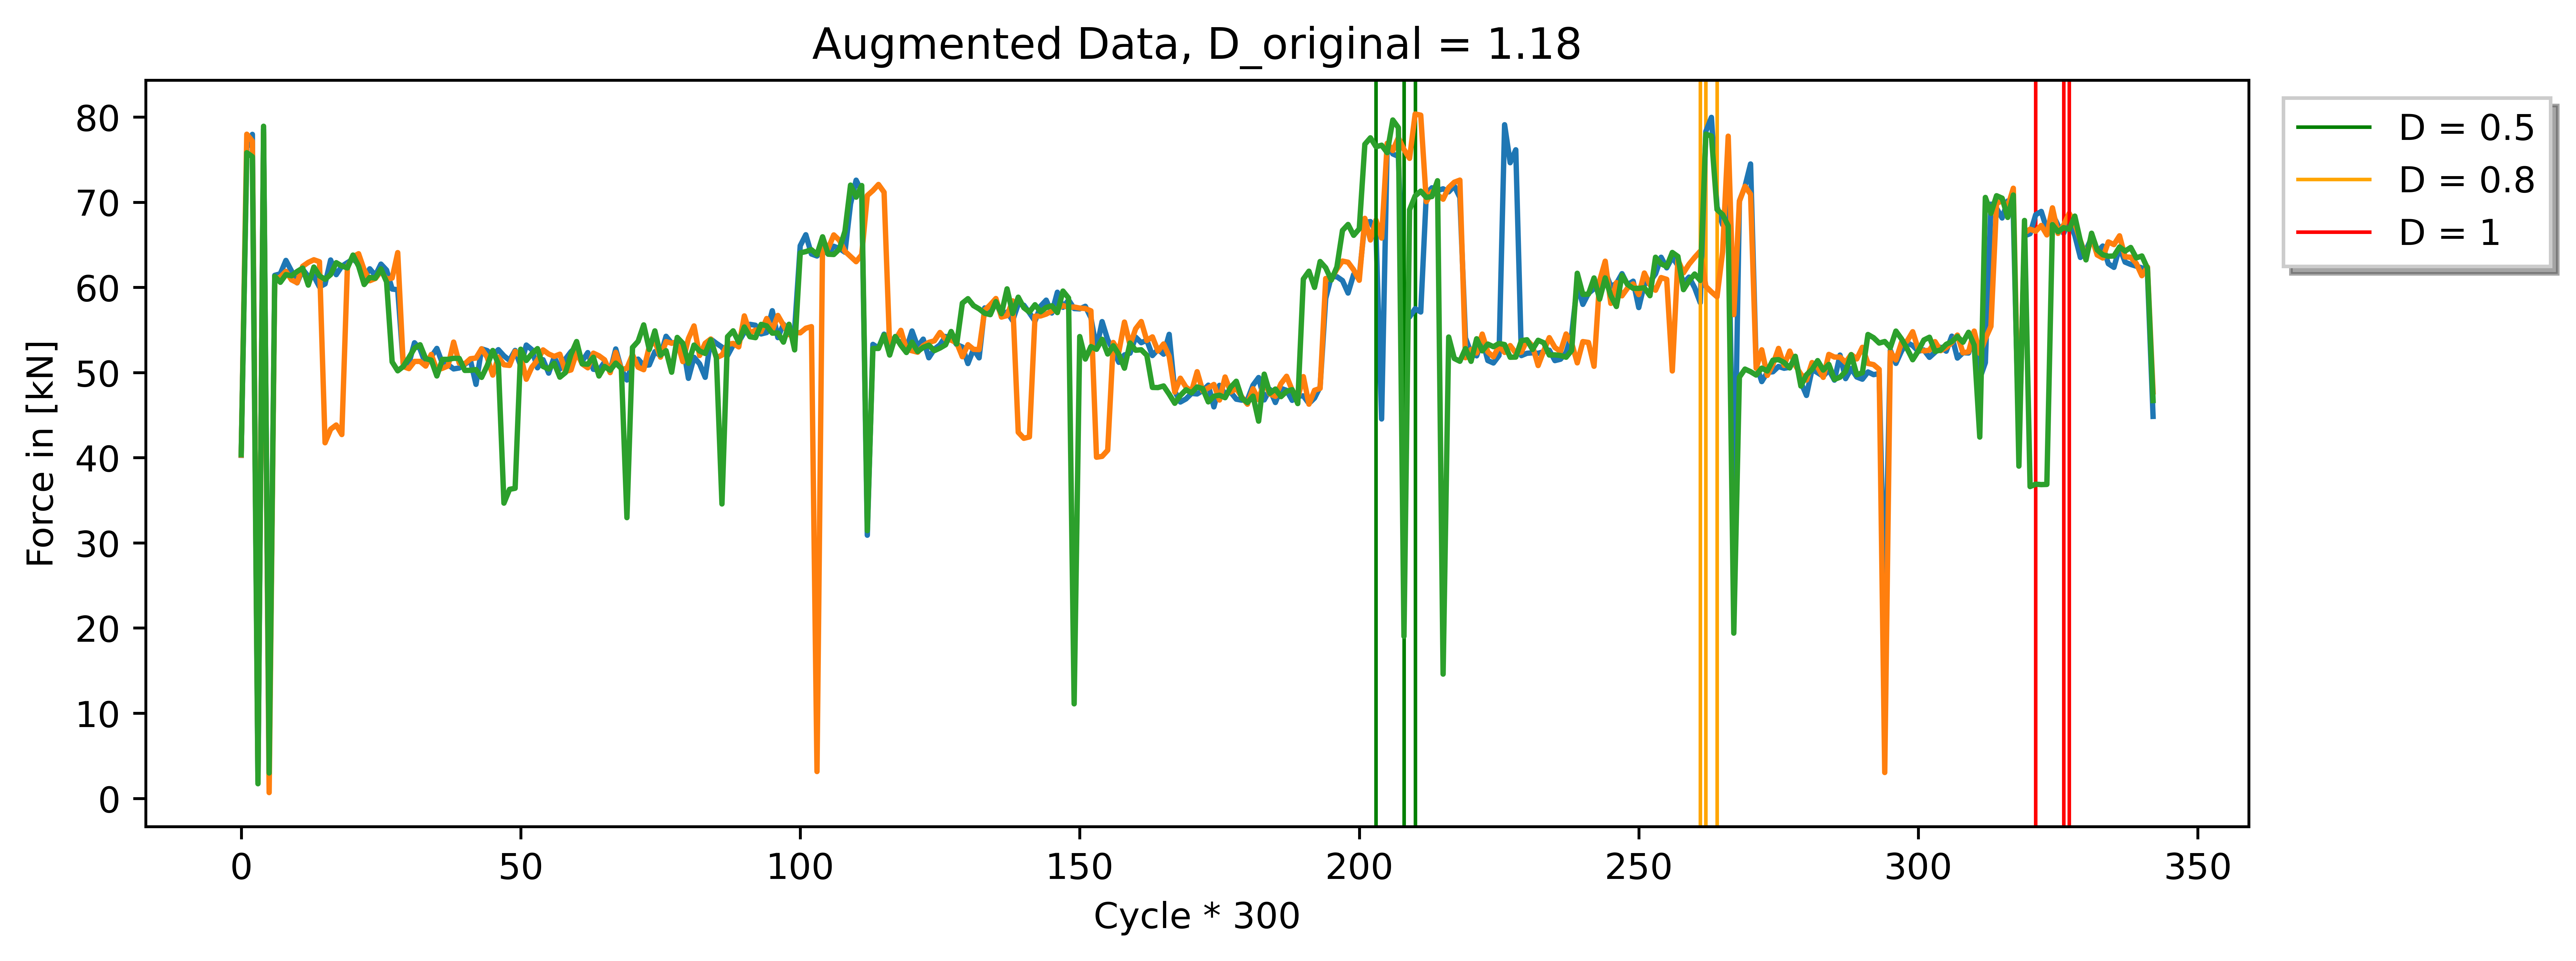
\includegraphics[width=1\linewidth]{IMGs/Augmented_5.png}
	\caption{Differences in augmented load sequences}
	\label{fig:3in1}
\end{figure}

Figure \ref{fig:allDA} shows all performed DA-steps in a schematic diagram.

\begin{figure}[H]
	\centering
	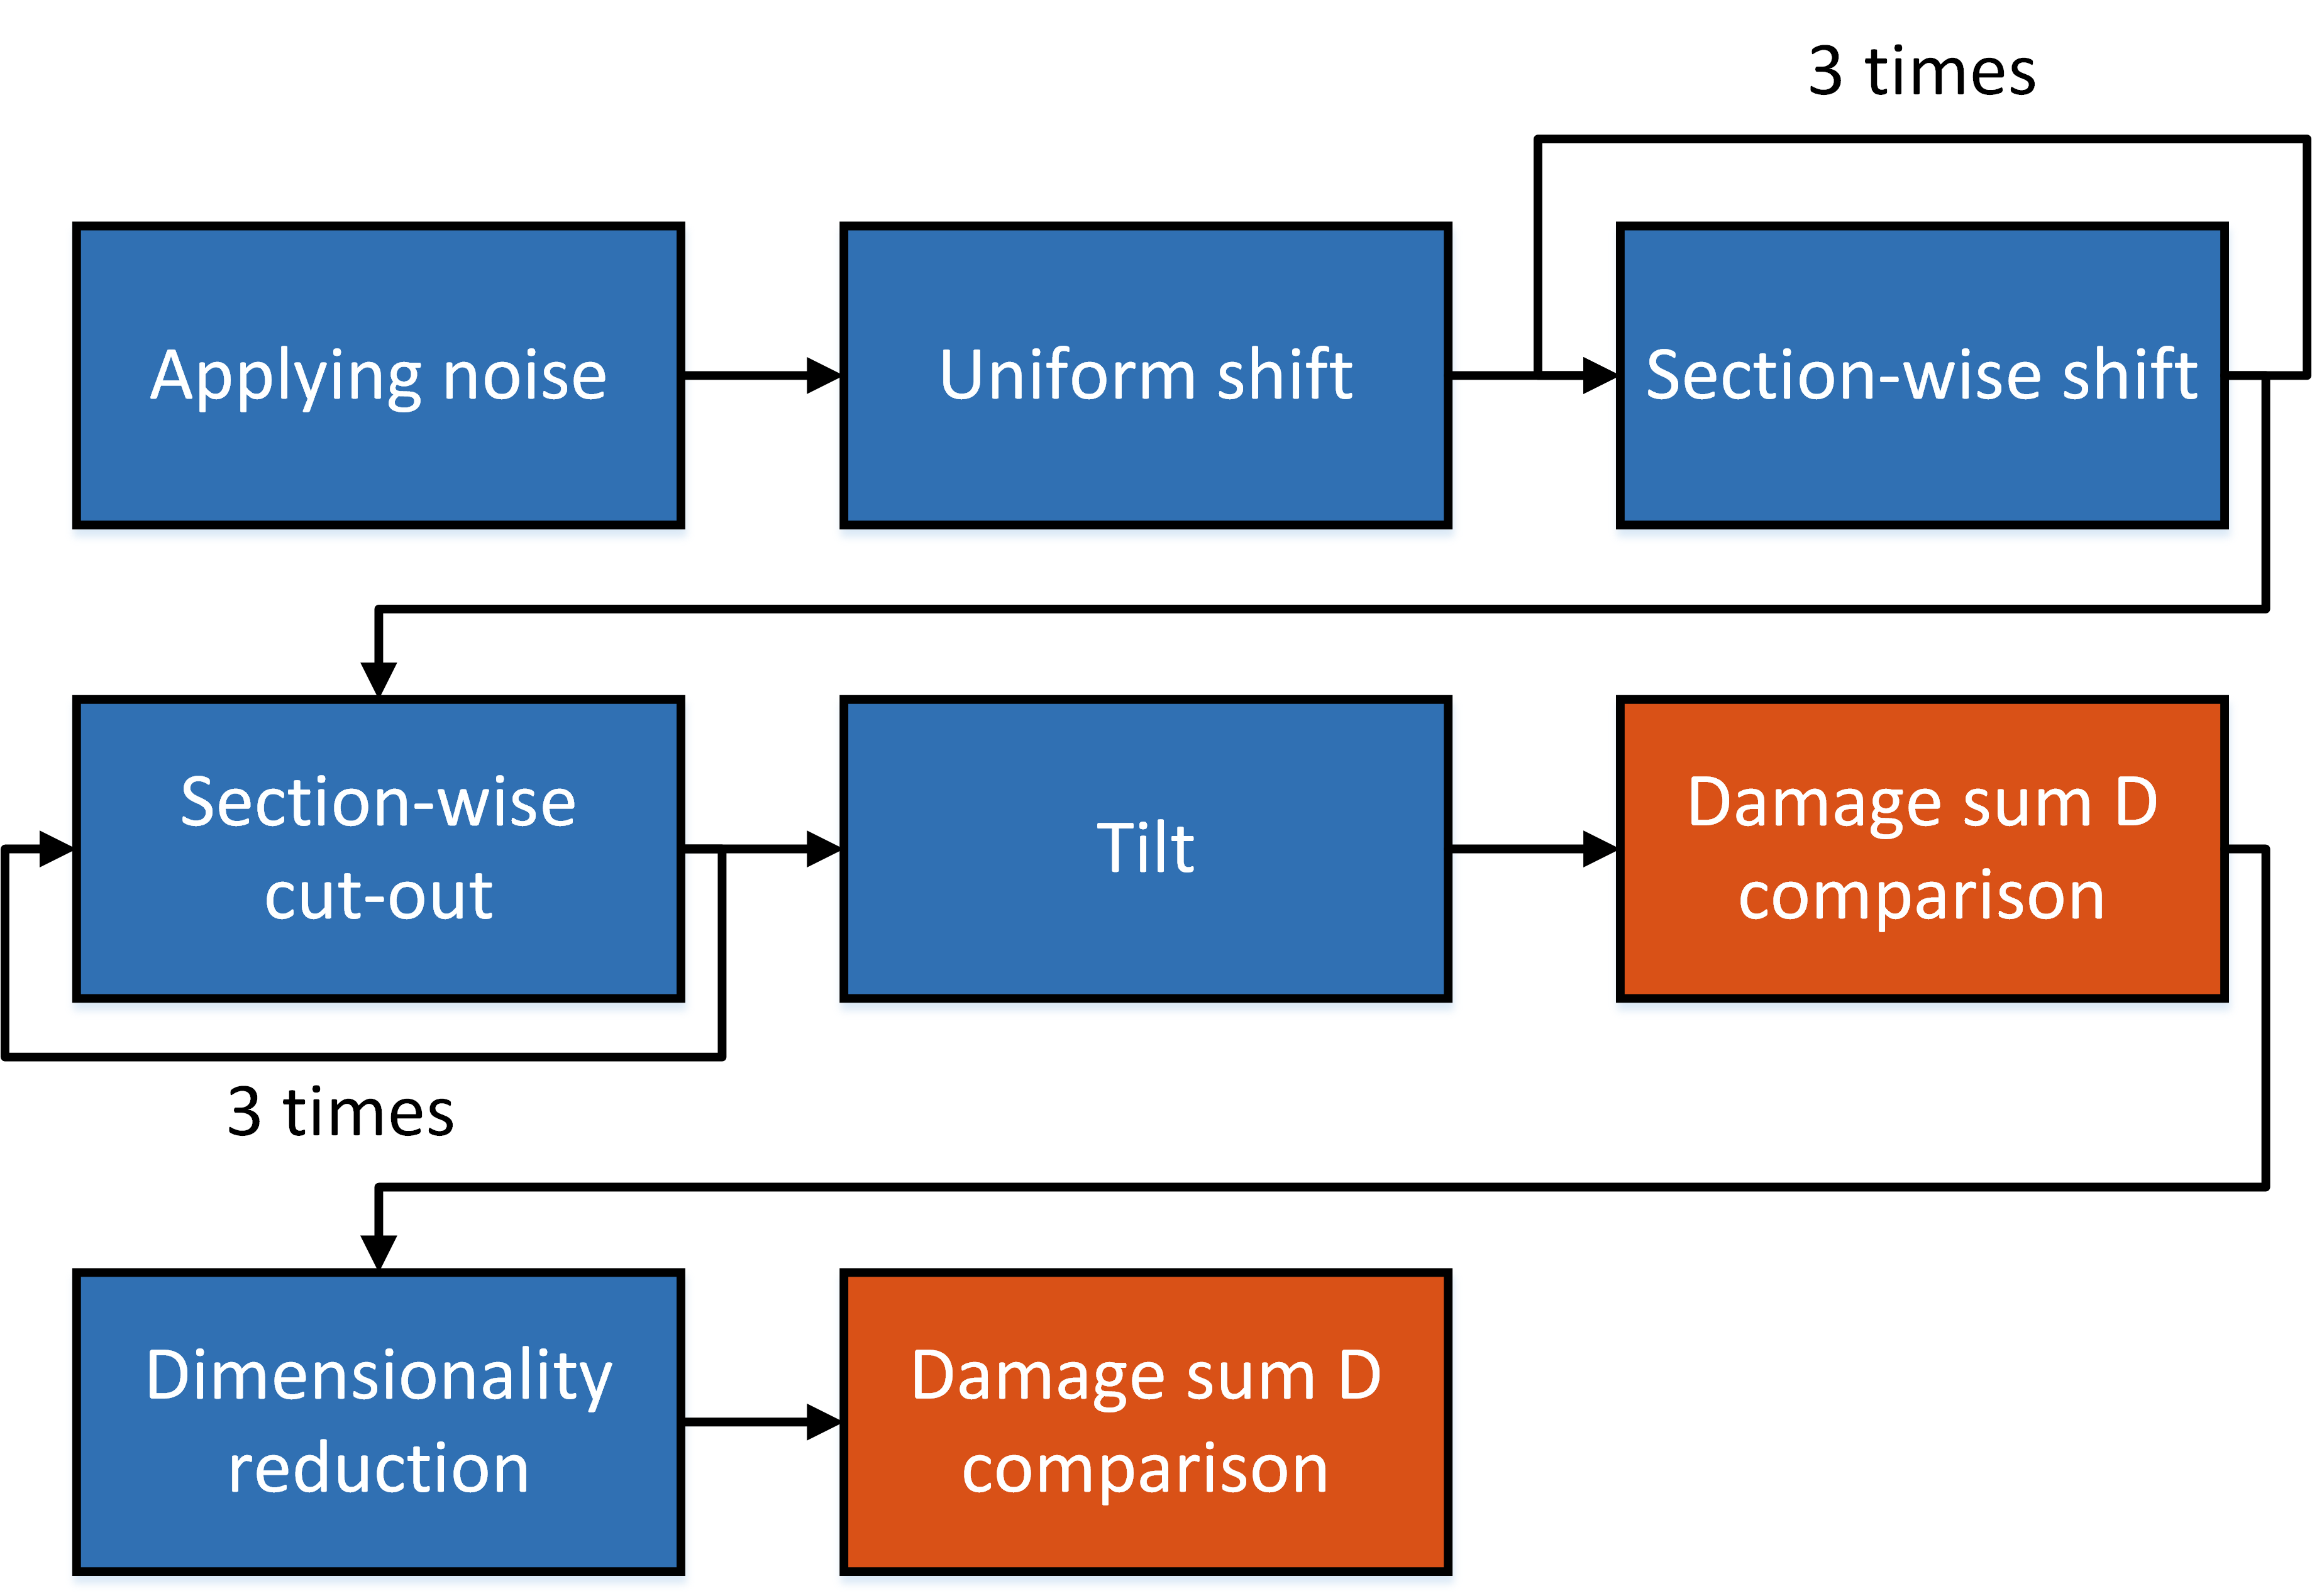
\includegraphics[width=0.7\linewidth]{IMGs/Augmentation.png}
	\caption{Augmentation procedure}
	\label{fig:allDA}
\end{figure}

From the original 14 load sequences, on average, 200 augmented sequences are created. This means that 150 out of 350 load sequences do not meet the requirement that the damage~sum~D is not significantly different from the original load sequence. 
The goal is to augment the load sequence as much as possible while at the same time retaining the damage sum D and the characteristics of every load sequence. 


The average length of the load sequences after dimensionality reduction is 320 data points. The shortest load sequence has 66 data points, and the longest one has 1000 data points. This large difference comes from the fact that load sequence number 4 (see table \ref{DamageSUMS}) failed at a very high damage sum D while load sequence number 12 failed at a very low damage sum D.
\newpage
One challenge when applying the selected DA-techniques is that a small alteration in damage sum~D in load sequences can have a very large relative change compared to the original damage~sum~D. For example, sequence number 12 has a damage sum D of 0.73 and after DA a damage sum of 0.82. The absolute change in damage sum D is 0.09. But when looking at the ratio, (0.82/0.73 = 1.12) the augmented load sequence is not accepted into the training set. Thus, almost no augmented elements of sequence 12 are present in the training data set. The same problem is present, but less pronounced, with other sequences with low damage sum D.



\section{Training and Validation}
When having an unfinished load sequence that needs to be analyzed, chapters \ref{prep_class} and \ref{PrRe} explain that the classifier and regressor are trained specifically for that individual load sequence. This is because the training set is adapted to the current damage sum D of the unfinished load sequence.

For testing purposes, the damage sum D (which would have come from the unfinished load sequence) is manually set to 0.6
The success of the classifier and regressor is analyzed by splitting the data into a test-set and training-set. 
20~\% of the data is given to the test-set and~80~\% to the training-set.

The training-set contains on average: 50 elements of class -1, 30 elements of class 0 and 90 elements of class 0. This ratio comes directly from the distribution of the original data-set where most load sequences failed at a damage sum D higher than 1.1.

\subsection{Training of the Classifier}
To train the classifier, the augmented load sequences are loaded into one list of arrays. The label of the array is extracted from the names of the files created in the augmentation step and also stored in an array. 

The load sequences are in their full length and need to be shortened to the length where the damage sum D is equal to 0.6 to be comparable to the unfinished load sequence. Note that in this case, the unfinished load sequence corresponds to the sequences in the test-set. 


The dataset is divided into a training- and test-set with the help of a prebuilt train-test-split function taken from \cite{SKlearn}. Table \ref{methods} shows the ten classifiers that are implemented to compare their individual performance:

%\begin{itemize} 
%	\itemsep-0.5em 
%	\item KNeighborsTimeSeriesClassifier \cite{tslearn}
%	\item TimeSeriesSVC \cite{tslearn}
%	\item AdaBoostClassifier \cite{SKlearn}
%	\item GradientBoostingClassifier \cite{SKlearn}
%	\item RandomForestClassifier \cite{SKlearn}
%	\item XGBoost\cite{XG}
%	\item Neural Net \cite{SKlearn}
%	\item GaussianNB \cite{SKlearn}
%	\item QuadraticDiscriminantAnalysis \cite{SKlearn}
%	\item KNeighborsClassifier \cite{SKlearn}
%\end{itemize}


\begin{table}
	\begin{center}
		\begin{tabular}{|| l | l ||}\hline
			\rule{0pt}{2ex}1) KNeighborsTimeSeriesClassifier \cite{tslearn} & 2) TimeSeriesSVC \cite{tslearn}\\	\hline
			3) AdaBoostClassifier \cite{SKlearn} & 4) GradientBoostingClassifier \cite{SKlearn} \\ \hline
		5) RandomForestClassifier \cite{SKlearn} & 6) XGBoost\cite{XG}\\ \hline
			7) Neural Net \cite{SKlearn} & 8) GaussianNB \cite{SKlearn} \\ \hline
			9) QuadraticDiscriminantAnalysis \cite{SKlearn} & 10) KNeighborsClassifier \cite{SKlearn} \\ \hline
		\end{tabular}
		\caption{Implemented Methods for Classification}
		\label{methods}
	\end{center}
	\vspace{-4mm}
\end{table}
\newpage

Only the "KNeighborsTimeSeriesClassifier" and "TimeSeriesSVC" are capable of accepting input vectors that have a varying length. To use the remaining classifiers, the load sequences are brought to the same length by pre-pending zeros, so that the overall length is equal to the longest sequence. Note that the length is defined by the longest load sequence in both of the datasets (train- and test-set).




\subsection{Training of the Regressor}
The training set of the regressor is dependent on the result of the classifier. For analysis purposes, the performance is analyzed by predicting the SOH on all three possible classes. 

For a predicted class, for example class 1, only the load sequences are loaded that belong to that class. In each load sequence, a random point is selected, and the label is calculated by the label function as described in chapter \ref{PrRe}. The array is shortened to the randomly selected point and stored in a list. The corresponding label is stored in an array. From each load sequence, four such frames are selected.

The analyzed regressors for predicting the SOH are:
\begin{itemize} 
	\itemsep-0.5em 
	\item AdaBoostRegressor \cite{tslearn}
	\item RandomForestRegressor \cite{tslearn}
\end{itemize}

The library "TSlearn" \cite{tslearn} contains a regressor called "TimeSeriesSVR", which is capable of working with input vectors of different lengths. The issue is that the maximum length must not exceed 450 elements. Because some arrays exceed this length, only two selected regressors from SKlearn \cite{SKlearn} are tested. To bring all arrays to the same length, a zero-padding method is employed, just as in the classification approach.

\section{Analysis and Discussion of the Results}
\subsection{Results of Classification}
To get an accurate evaluation of the performance of the selected classifiers, each model is trained and tested 25 times on a different data-set. This means that the data augmentation step of all load sequences is performed every time before the training of a classifier starts.
By doing that, the train- and test-set are varied. Another way to get the average performance is k-fold cross-validation as described in chapter \ref{KCV}. Due to the ability to generate variations in data, the k-fold cross-validation approach is disregarded. By averaging the performance over 25 iterations on the test-set, an accurate average performance is calculated. 

The average individual performance of all tested classifiers is shown in figure \ref{fig:avgperf}. 
A score of 1 means a correct classification of all sequences. The value in the plot is a ratio of correctly predicted classes to all predictions.

\begin{figure}[H]
	\centering
	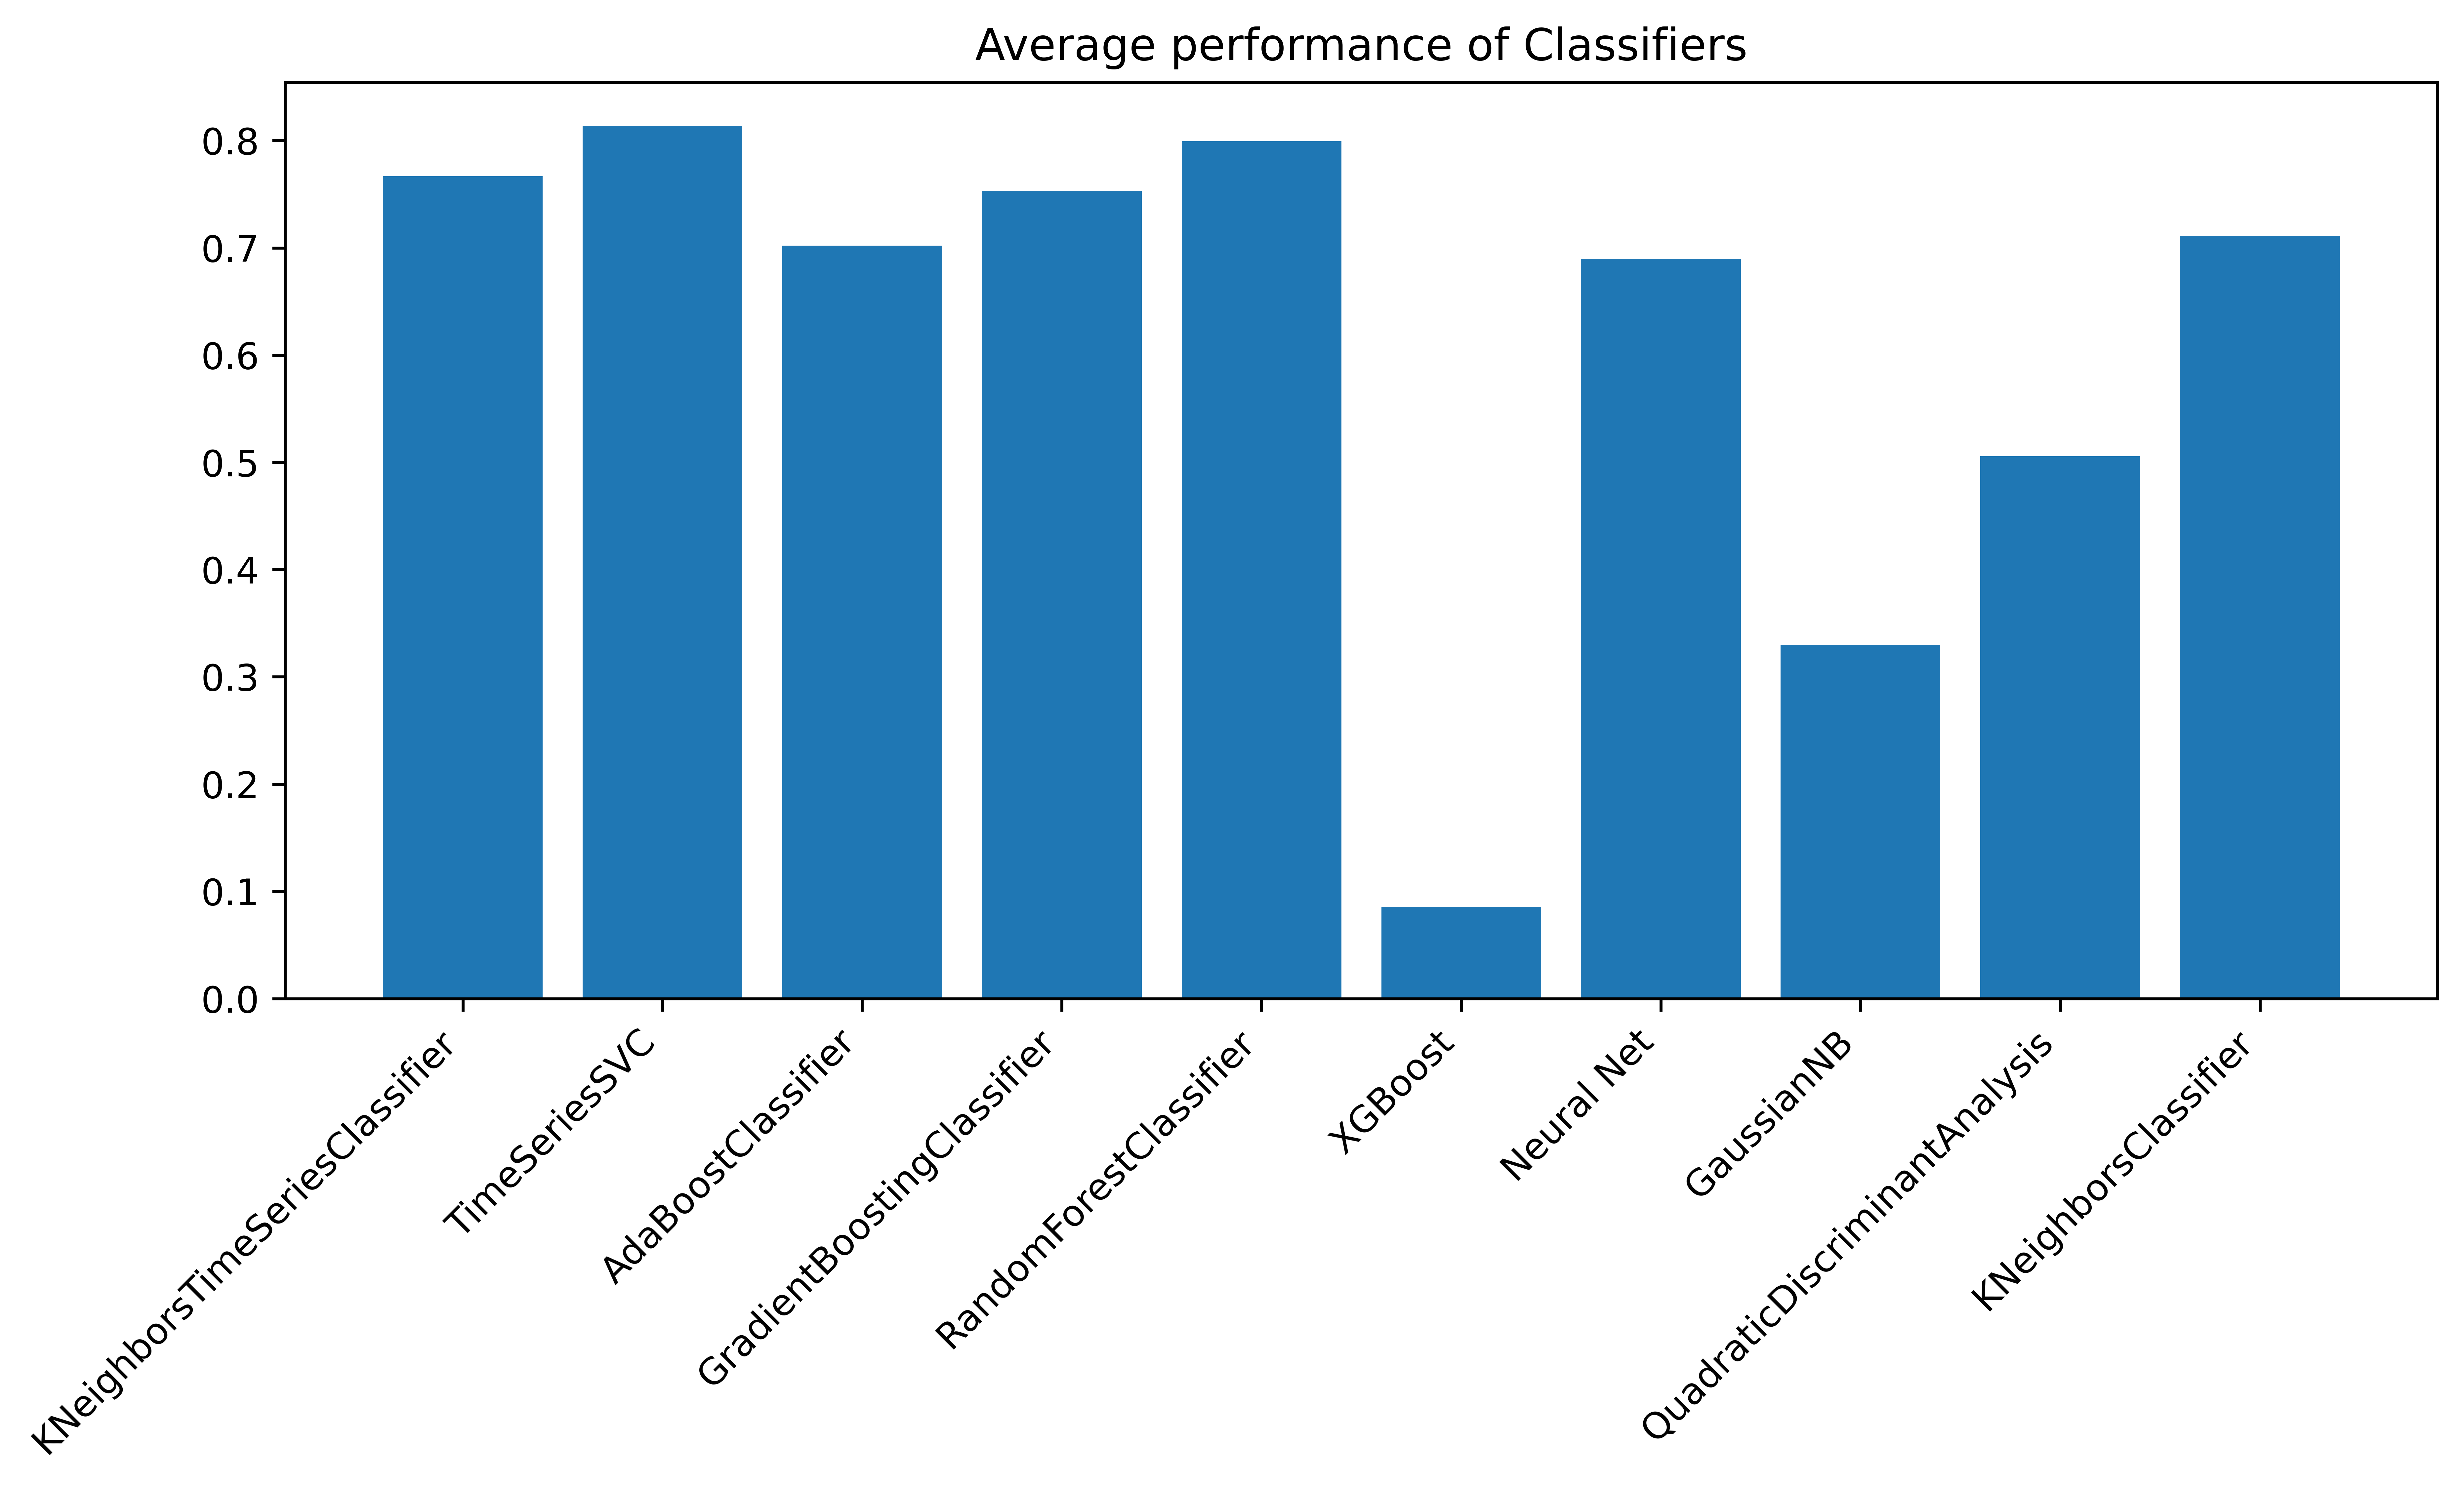
\includegraphics[width=1\linewidth]{IMGs/Average_performance_CLASS.png}
	\caption{Average performance of predicting the correct class for each classifier}
	\label{fig:avgperf}
\end{figure}

When looking at the results, most of the classifiers are capable of predicting the correct class for the load sequences in the test-set of up to 80 \% of the time. 
It is noticeable that the two first classifiers that are working with input vectors of varying length are as capable as the classifiers that require constant dimensions. The best performance is achieved by "TimeSeriesSVC" from \cite{tslearn} which predicted the correct class 81.3 \% of the time. The worst performance was achieved by "XGboost" with only 8.5 \%. This is a noticeable result because an average score of 33 \% is expected when the labels are predicted at random. 

Table \ref{score} shows the analyzed classifiers sorted by performance. 

\begin{table}
	\begin{center}
		\begin{tabular}{|| l | l ||}
			\hline
			\rule{0pt}{2ex}Classifier & Average performance\\
			\hline
			\hline
			\rule{0pt}{2ex}TimeSeriesSVC & 81.3 \%\\	\hline
			RandomForestClassifier & 79.9 \% \\ \hline
			KNeighborsTimeSeriesClassifier & 76.6 \%\\ \hline
			GradientBoostingClassifier & 75.3 \%\\ \hline
			KNeighborsClassifier & 71.1 \%\\ \hline
			AdaBoostClassifier & 70.1 \% \\ \hline
			Neural Net & 68.9 \% \\ \hline
			QuadraticDiscriminantAnalysis & 50.5 \% \\ \hline
			GaussianNB & 32.9 \% \\ \hline
			XGBoost & 8.5 \% \\ \hline

		\end{tabular}
		\caption{Average performance of classifiers}
		\label{score}
	\end{center}
	\vspace{-4mm}
\end{table}
\newpage
\subsection{Results of Regression}

The regressors are trained for each possible class and evaluated on their performance. The performance is averaged over 25 trainings to get an accurate average score for the regressors. The score is obtained by averaging the mean-square error of the prediction for each class.

Figure \ref{fig:avgperf_reg} shows the result of the averaged training. The predictions of the correct SOH in classes -1 and 1 are more accurate than in class 0. One possible explanation for this performance is the previously mentioned disparity in number of elements in each class. Class 1 and class~-1 have more data points and thus allow for a better prediction. Both regressors show similar performance in each class.

\begin{figure}[H]
	\centering
	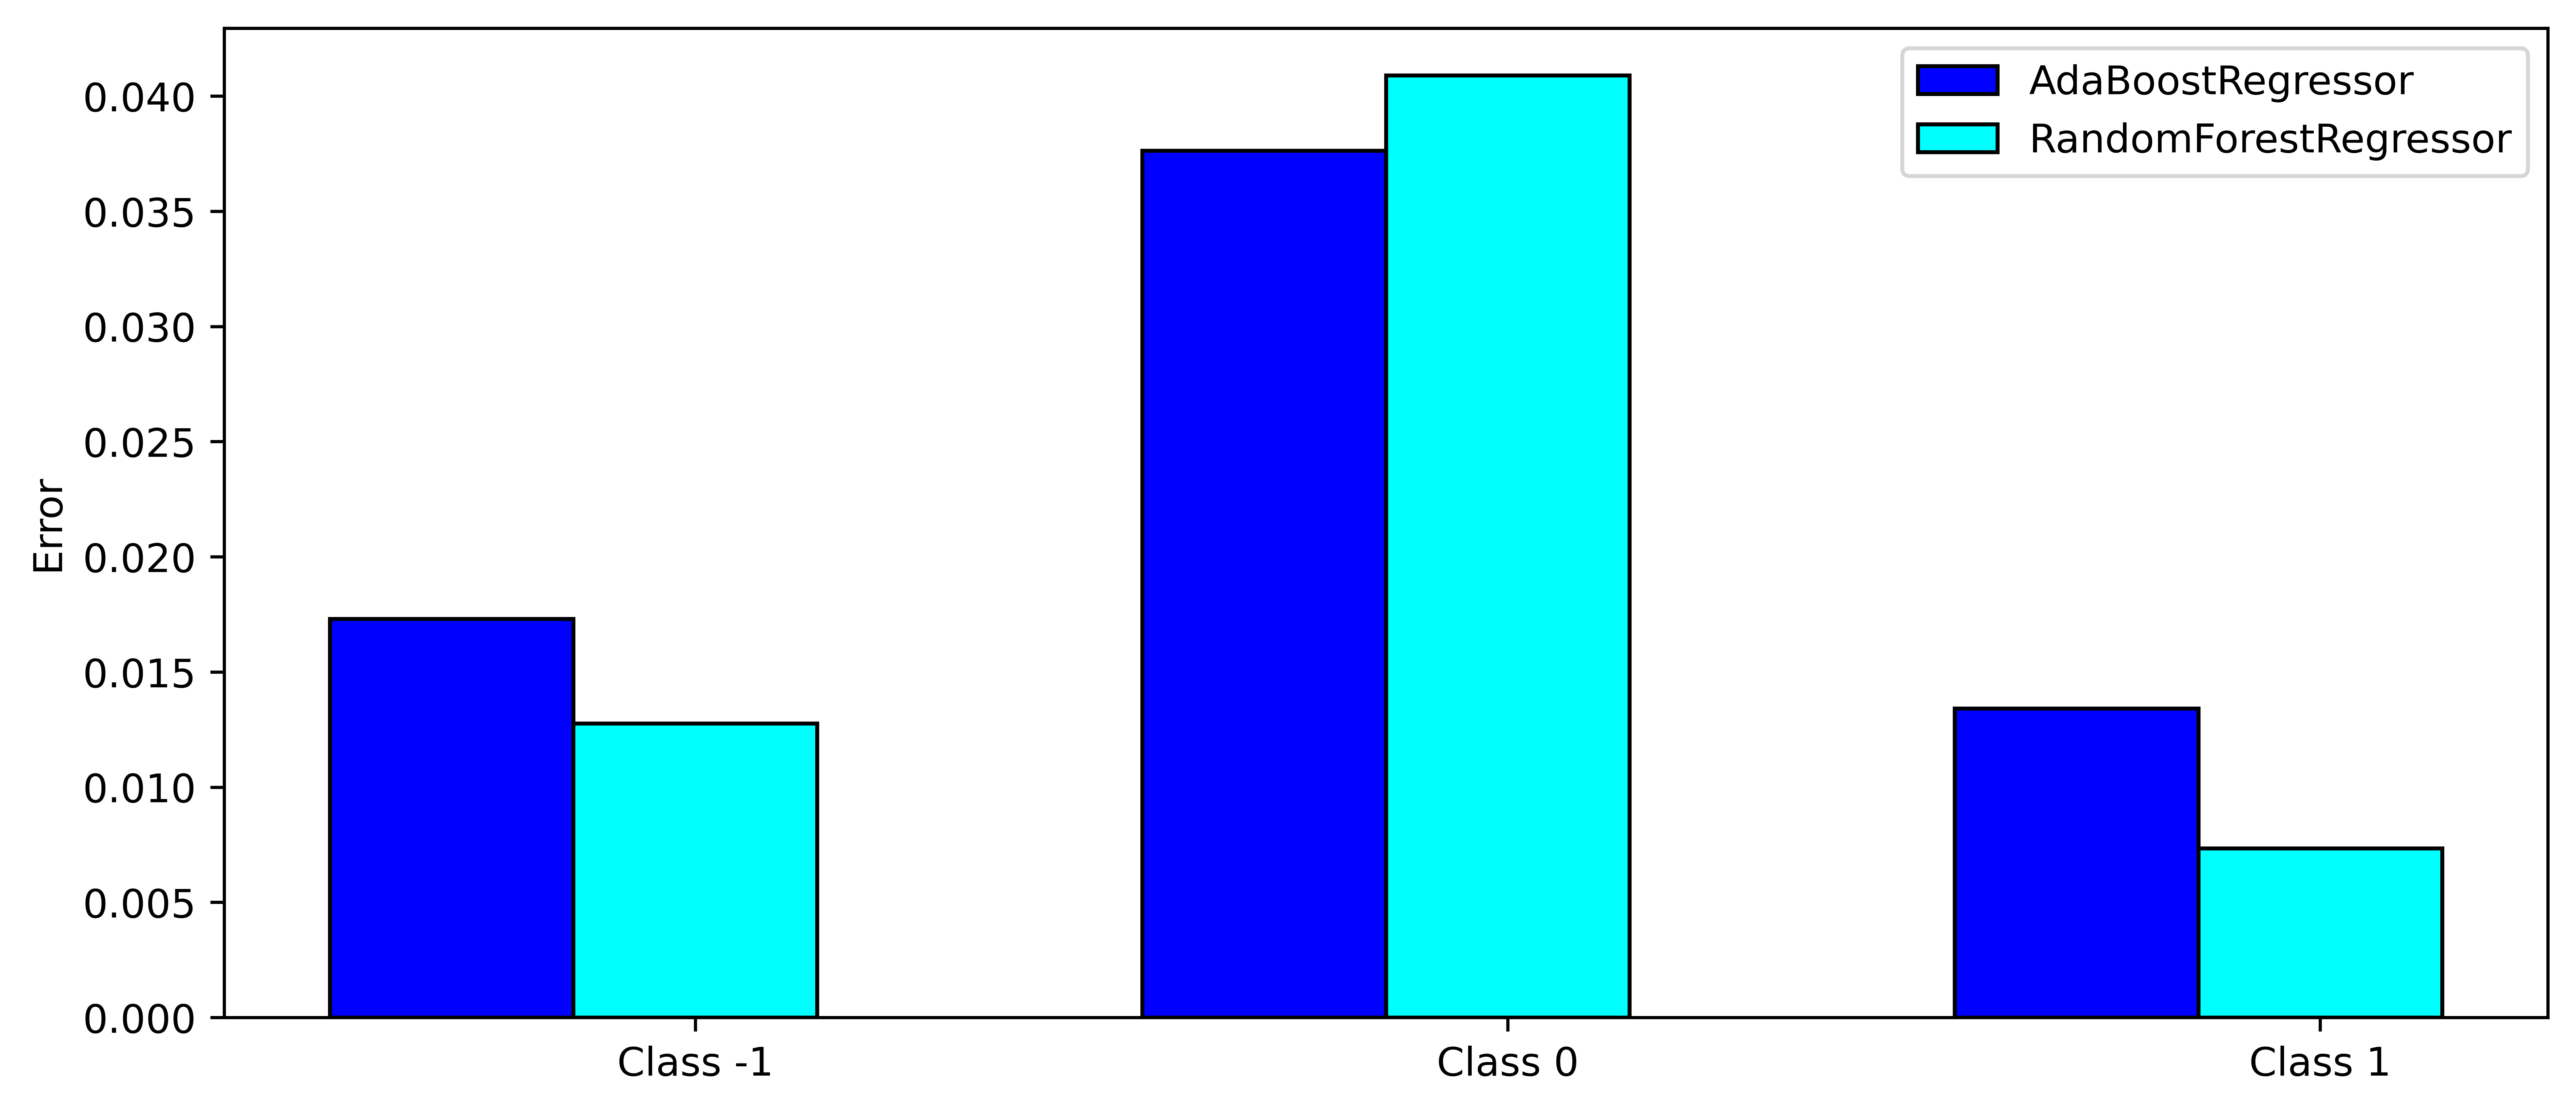
\includegraphics[width=1\linewidth]{IMGs/Average_performance_REG.png}
	\caption{Average performance of each regressor for predicting the SOH in each class}
	\label{fig:avgperf_reg}
\end{figure}
\subsection{Critical Discussion of Results}

The tested methods prove to return accurate results in classification and regression. One possible reason for that is that the implemented DA steps do not alter the structure of the loading sequence enough to be seen as a completely different load sequence. Thus, if an augmented element of a load sequence is in the training-set and testing-set, the ML models do not need to have the ability to generalize to predict the correct class for that sequence. 

When predicting the SOH the inputs from test- and training-set have significant differences in length. Thus the same problem of over-fitting is not present. For a more accurate result and better performance of the ML models more data is necessary. As mentioned before, only~14~load sequences were available which makes the training of the ML models to generalize well, a challenging task.   

\afterpage{\null\newpage}
% !TeX spellcheck = en_US 
\chapter{Conclusion}\label{conc}
\section{Summary}
Machine elements depend on correct dimensioning to function as expected over their course of life. So far, the most prominent method for fatigue strength analysis is the Miner rule, which is accepted as an international standard. The downside of the Miner rule is that the order of the occurring loads is not taken into account. Regarding the current state of research, no theory has been developed that takes the order (history) of load into account and is easily transferable between machine elements.
The goal of this thesis is to develop a method that is able to provide a confidence value in the calculated state-of-damage by specifically considering the history of the loads that a machine element is subjected to. This thesis proposes a method that can classify a load sequence into one of three possible classes, depending on the effect of the load history. Further, a second indicator called state-of-health is added to analyze how much a machine element is worn down. With the combination of these two values, the state-of-damage is now supplied with more information and can be viewed from a different perspective. 
The provided load sequences are augmented with various techniques to form an enriched data-set. The analyzed classification methods return very promising results and are capable of correctly classifying a load sequence in 80~\% of cases. 
The selected regression models are also capable of predicting the state-of-health with very low error margins.
In conclusion, this method provides a very capable and robust alternative to nonlinear damage accumulation models that provides accurate results and is easily applicable to every machine element.  


\section{Outlook}
One of the most important aspects when it comes to ML approaches is the amount and quality of the data. To get an even more accurate result of the predicted classes and SOH, the supply of more data is the most important step. Further, it is possible to add more DA methods to increase the model's ability to generalize. 

Regarding the separation into classes, the proposed method only divides the load sequences into three distinct groups (Class -1, Class 0, Class 1). For a more precise prediction, it could be beneficial to increase the number of classes to get an understanding of how much the Miner rule is deviating from the predicted damaging effect of the load sequence.

Additionally, further models like RNNs can be implemented that can predict the class and SOH on the fly. This could be a form of condition monitoring that could give an even more accurate prediction and is also not dependent on iteratively retraining for a different damage sum D. Another option is the implementation of Bayesian Neural Networks that quantify the uncertainty in the predicted class. 

A further area of possible research is the prediction of the SOH not with a simple linear interpolation but with different functions that can depend on the output of the previous classification. Optionally, the label function can be a scaled Miner rule so that the label function has the value~1 at the end of the sequence and includes some knowledge about the Miner rule.  

\afterpage{\null\newpage}

%...

%==== Literaturverzeichnis ====
\clearpage
\chapter*{\bibname}
\markboth{\bibname}{}
\insertbib
\listoffigures
\listoftables
% In der Bib sollte für Normen und Richtlinien als Type MANUAL und Webseite als ONLINE eingegeben



%\phantomsection\label{sec:literaturverzeichnis}
%\bibliography{litbib}
%\addcontentsline{toc}{section}{\bibname}
\clearpage

%=========================================================
%==== Anhang ====

% Var1: ueber \Anhang
%\Anhang
%\section{Sektionsüberschrift}
\label{sec:Anochmalsektion}
\textcolor{red}{!!! Hinweis !!!: Anhänge werden als \textbackslash section definiert.}\\
%
Literatur \cite{DIN3990} \cite{testweb}
%
%===================
\subsection{Subsektion}
\label{sec:Asubsektion}
%
\begin{figure}
	\centering
	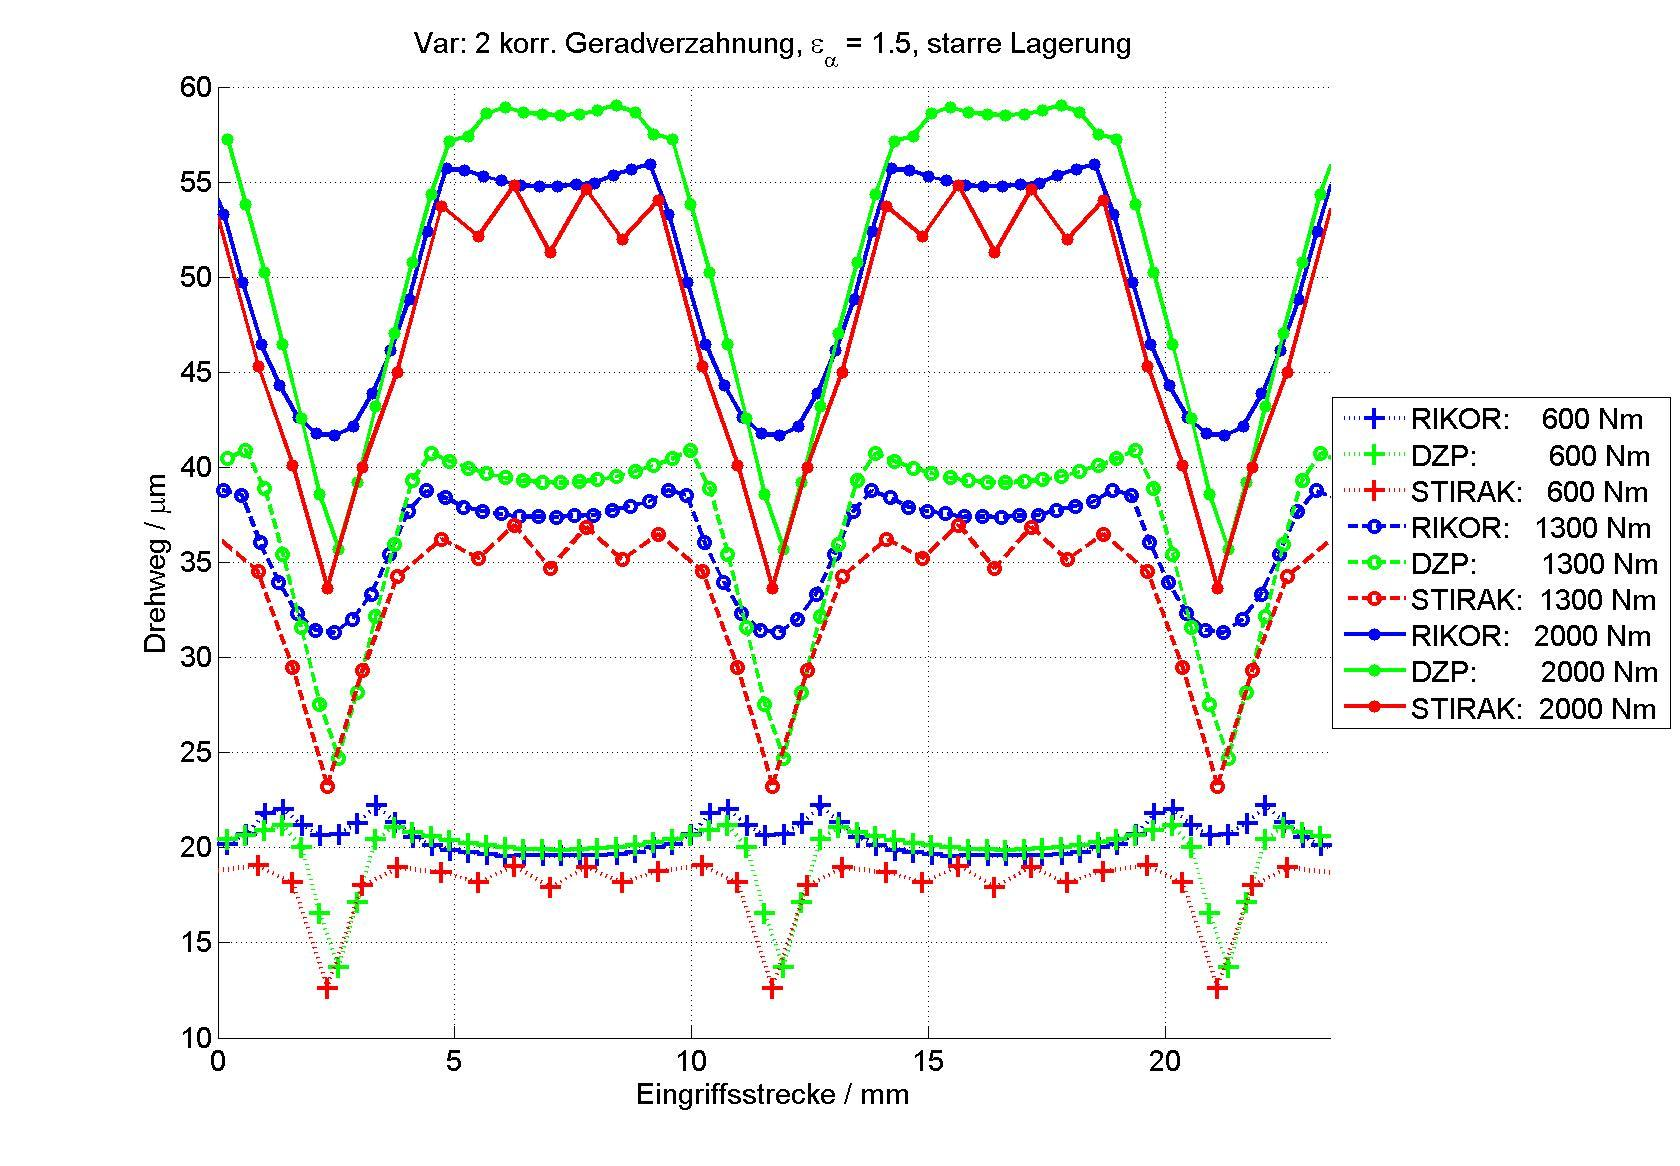
\includegraphics[width=0.5\textwidth]{_ltx/Beispiel.jpg}
	\caption{Dies ist ein wunderschönes Bild, das auch aus einer Quelle und so weiter stammen kann \cite{Niemann01}. Deshalb sind Bildunterschriften so einfach möglich.}
	\label{fig:Abeispiel}
\end{figure}
%
%----------------------
\subsubsection{Subsubsektion}
\label{sec:Asubsubsektion}
%
\textbf{fett} \textit{italic} \textsl{sl} \textsc{Kapitälchen}\\
Formel im Text $\varepsilon$ bla
\begin{equation}
	a^2 + b^2 = c^2
	\label{eq:pytagoras}
	\end{equation}
%
\begin{Gleichungsparameter}
\Gleichungparaeintrag{a}{ - }{Ankathete}{b}{ - }{Gegenkathete}  
\Gleichungparaeintrageinfach{c}{ - }{Hypotenuse}
\end{Gleichungsparameter}
%
%---------
\paragraph{Paragraph}
\label{sec:paragraph}
%
\begin{equation}
	\eta = \dfrac{P_{Ab}}{P_{An}} = \dfrac{P_{An}-P_{V}}{P_{An}}
\end{equation}
%
\begin{Gleichungsparameter}
\Gleichungparaeintrag{\eta}{ - }{Wirkungsgrad}{P_{Ab}}{ kW }{Abtriebsleistung}  
\Gleichungparaeintrag{P_{An}}{ kW }{Antriebsleistung, die auch einen Zeilenumbruch erlaubt}{P_V}{ kW }{Verlustleistung} 
\end{Gleichungsparameter}

Wie man in \eqref{eq:pytagoras} sieht, bzw wie man in \seqref{eq:pytagoras}

\begin{table}
\caption{test}
\end{table}

%---------
\paragraph{Paragraph}
\label{sec:paragraph}
%
\begin{equation}
	\eta = \dfrac{P_{Ab}}{P_{An}} = \dfrac{P_{An}-P_{V}}{P_{An}}
\end{equation}
%
\begin{Gleichungsparameter}
\Gleichungparaeintrag{\eta}{ - }{Wirkungsgrad}{P_{Ab}}{ kW }{Abtriebsleistung}  
\Gleichungparaeintrag{P_{An}}{ kW }{Antriebsleistung, die auch einen Zeilenumbruch erlaubt}{P_V}{ kW }{Verlustleistung} 
\end{Gleichungsparameter}

Wie man in \eqref{eq:pytagoras} sieht, bzw wie man in \seqref{eq:pytagoras}



% Var2: ueber \appendix; !!! usepackage{appendix} % verwenden !!!
%\appendix
%\phantomsection
%\addcontentsline{toc}{section}{Anhang}

\end{document}